%\documentclass[11pt, book]{report}  %can try book instead 	% use "amsart" instead of "article" for AMSLaTeX format
\documentclass[11pt]{report}  %can try book instead   % use "amsart" instead of "article" for AMSLaTeX format
\usepackage[margin = 0.7in, bmargin = 1.1in, tmargin = 0.9in]{geometry}                		% See geometry.pdf to learn the layout options. There are lots.
\geometry{a4paper}                   		% ... or a4paper or a5paper or ... 
%\geometry{landscape}                		% Activate for rotated page geometry
\usepackage[parfill]{parskip}    		% Activate to begin paragraphs with an empty line rather than an indent
\usepackage{graphicx}				% Use pdf, png, jpg, or eps§ with pdflatex; use eps in DVI mode
								% TeX will automatically convert eps --> pdf in pdflatex		
\usepackage{amssymb}
\usepackage{amsmath}
\usepackage{amsmath,mathtools}
\usepackage{array}
\usepackage{tabu}
\usepackage{bm}
\usepackage{wrapfig}
\usepackage{multirow}
\usepackage{physics}
\usepackage{hyperref}
\usepackage{listings}
\usepackage[utf8]{inputenc}
\usepackage[T1]{fontenc}
\usepackage{lmodern}
\usepackage{graphicx}
\usepackage{caption}
\usepackage{floatrow}
\usepackage{subfig}
\usepackage{multicol}
\usepackage{xcolor}
\usepackage{pagecolor}
\usepackage{lipsum}  
\usepackage{mdframed}
\usepackage{verbatim}
\usepackage{slashed}
%\usepackage[compat=1.1.0]{tikz-feynman}
%\usepackage{animate}


\newcommand{\G}{\mathcal{G}}
\newcommand{\D}{\mathcal{D}}
\newcommand{\E}{\mathcal{E}}
\renewcommand{\S}{\mathcal{S}}
\newcommand{\M}{\mathcal{M}}
\newcommand{\K}{\mathcal{K}}
\renewcommand{\L}{\mathcal{L}}
\newcommand{\R}{\mathcal{R}}
\renewcommand{\P}{\mathcal{P}}
\newcommand{\vp}{\varphi}
\newcommand{\T}{\mathcal{T}}
\newcommand{\A}{\mathcal{A}}
\newcommand{\bs}{\boldsymbol}
\newcommand{\rspace}{\mathbb{R}}
%\newcommand{\dd}{\mathrm{d}} % is included in physics package??

\newcommand{\mL}{\mathcal{L}} 
\newcommand{\xt}{\tilde{x}}    
\newcommand{\pN}{{}_{\perp}N}
\newcommand{\rmi}{{\rm i}}


\definecolor{purple}{RGB}{38,0,75}
\pagecolor{white}
\color{black}

%SetFonts

%SetFonts
\usepackage{subfiles} % Best loaded last in the preamble

\numberwithin{equation}{section}
\pagenumbering{gobble}
\title{Third Term Report}
\author{Robin Croft}
%\date{}	
\begin{document}
\begin{titlepage}
\pagenumbering{gobble}
  \centering
  
  \centering
  {\scshape\LARGE Cambridge University \par}
  \vspace{1cm}
  {\scshape\Large Doctoral Thesis \par} 
    \vspace{2cm} 
    \hline
    \vspace{0.3cm}
  {\Large\itshape \par}
  {\huge\bfseries On the Simulation of Boson Stars in General Relativity\par} \vspace{0.3cm}
  \hline
  \vfill
   Author: Robin Croft
\vfill
  Supervisor: Dr. Ulrich Sperhake
  \vfill

    \begin{figure}[h!]
  \centering
  \subfloat{
\includegraphics[width=0.25\textwidth]{uni_logo.png}\label{fig:f1}}
\end{figure}


% Bottom of the page
 % {\large \today\par}
\end{titlepage}						% Activate to display a given date or no date
\tableofcontents
\newpage
\pagenumbering{arabic}





\chapter{Introduction to Differential Geometry and General Relativity}



%\newpage
%\pagenumbering{arabic}


\section{Introduction}
\subsection{Introduction to Compact Objects and Boson Stars}
The first non flat solution to Einstein's equation found was that of the spherically symmetric, static and asymptotically flat vacuum spacetime by Karl Schwarzschild in 1915. The solution was designed to be used outside a spherically symmetric, non-spinning, body of mass; however it turned out to provide use in describing black holes. This metric was then modified by Tolman, Oppenheimer and Volkov in 1939 to describe the non-vacuum case of a constant density neutron star. This turned out to give an unphysical estimate of $0.7 M_\odot$ for the upper limit of neutron star mass due to the equation of state. 

The study of compact exotic objects can be traced back to John Wheeler who investigated Geons in 1955 for their potential similarity to elementary particles. Geons are gravito-electromagnetic objects with the name arising from "gravitational electromagnetic entity". In 1968 David Kaup published [] describing what he called "Klein-Gordon Geons", nowadays referred to as boson stars. Importantly, boson stars are a localised complex Klein-Gordon configuration, with the real counterparts being unstable. Many variants such as (Spin 1) proca stars [], electromagnetically charged boson stars and many others have been studied. 

Interest in boson stars remains for many reasons. Given the recent discovery of the higgs boson, we know that scalar fields exist in nature and any gravitational wave signals created by compact objects could theoretically be detected with modern gravitational wave interferometers. Secondly, boson stars are a good candidate for dark matter haloes. Boson stars are also useful as a proxy to other compact objects in general relativity; there is a lot of freedom in the construction of different types of boson star and they can be fine tuned to model dense neutron stars for one example. The advantage this would have over simulating a real fluid is that the Klein Gordon equation is linear in the principal part meaning smooth data must always remain smooth; thus avoiding shocks and conserving particle numbers relatively well with less sophisticated numerical schemes. 

On a slightly different topic, collisions of boson stars could be a natural method to produce scalar hair around black holes which will be discussed later in more detail. 

\subsection{Conventions}
The conventions used in this report are Geometric units, $c=G=\hbar=1$, unless stated otherwise. The metric signature will always be $(-,+,+,+)$. Finally, for quantities such as the Ricci Scalar, which differ depending on wether they are elements of the full $3+1$ dimensional manifold $\M$ or a $3$D hypersurface $\Sigma$, standard letters $(R)$ represent the object belonging to the target space and calligraphic letters $(\R)$ correspond to the projected object.




\subsection{Differential Geometry}
We all learned Pythagerous theorem at school [INSERT PICTURE OF RIGHT ANGLED TRIANGLE], this is 2d. Generalise this to algebraic metric rather than constant kroneka delta metric. Give exmaple in spherical polars. Maybe use this to calculate areas/lengths. Maybe insert picture of sphere. Insert proof that root det g is needed for volume elment from transforming a generic metric from one coord system to another? maybe need to invoke diff forms?

Differential Geometry (DG) is the extension of calculus, linear algebra and multilinear algebra to general
geometries. Einstein’s Theory of Relativity is written using the language of DG as it is the natural
way to deal with curves, tensor calculus and differential tensor equations in curved spaces. For a basic
introduction to DG, we should start with a manifold $\M$ which is an $N$ dimensional space that locally looks
like $\rspace^N$, $N$ dimensional Euclidean space. This is important as at a point $p\in\M$ we can find infinitesimally
close neighbouring points $p + \delta p \in \M$. 

A real scalar function $f$ over $\M$ maps any point $p\in \M$ to a real number, this is denoted as
$f : p \rightarrow \rspace$. An important example of a set of scalar functions is the coordinate system $\phi$, $\phi : p \rightarrow \rspace^N$,
this is normally written $x^\mu$ where $\mu\in\{0,1,...,N-1\}$ is an index labelling the coordinate. The map $\phi$ is called a chart,
and unlike Euclidean space one chart may not be enough to cover the entire manifold; in this case a set
of compatible charts should be smoothly joined, collectively known as an atlas.

Now that functions have been discussed, the next simplest object we can discuss is a curve, or path, through $\M$. A curve $\Gamma$ is a set of smoothly connected points $p(\lambda)\in \M$ that smoothly depend on an input parameter $\lambda \in [\lambda_0,\lambda_1]$. This can be expressed in terms of coordinates as $x^\mu(\lambda)$ where $\phi:p(\lambda) \rightarrow x^\mu(\lambda)$. Differentiating a function $f$ along $\Gamma$ with respect to $\lambda$ gives
\begin{equation} \label{eq:dfdl}
\frac{\dd}{\dd \lambda}f(x^\mu(\lambda)) = \frac{\dd x^\nu}{\dd \lambda}\frac{\partial f(x^\mu)}{\partial x^\nu} = \frac{\dd x^\nu}{\dd \lambda}\partial_\nu f,
\end{equation}
where $\partial_\nu = {\partial}/{\partial x^\nu}$ and the Einstein summation convention was invoked, summing over all values of $\nu$. Equation~(\ref{eq:dfdl}) was derived independantly of the choice of $f$, therefore we can generally write
\begin{equation} \label{eq:ddl}
\frac{\dd}{\dd \lambda} = \frac{\dd x^\nu}{\dd \lambda}\partial_\nu.
\end{equation}
The operator $\dd/\dd \lambda $ can act on any function $f$ and return a new function $\tilde{f}$ over $\M$, formally this is written as $\dd/\dd \lambda (f) = \tilde{f}$ where $\tilde{f}:p\in\M\rightarrow \rspace$. We can also think of $\dd/\dd \lambda$ as a vector $\bs{X}$ with components $X^\mu=\dd x^\mu / \dd \lambda$ and basis vectors $\bs{e}_\mu:=\partial_\mu$ taken from Eq.~(\ref{eq:ddl}). The vector $\bs{X}$ can be written as $\bs{X} = X^\mu \bs{e}_\mu$ and can act on a general function $f$ over $\M$ as $\bs{X}(f) = X^\mu \bs{e}_\mu(f) = X^\mu \partial_\mu f$. 

Considering the set of all possible curves through a points $p\in\M$, the tangent vector components $\dd x^\mu / \dd \lambda$ span an $N$ dimensional space with basis $\bs{e}_\mu = \partial_\mu$; this space is called the tangent space and is denoted as $\T_p(\M)$. For the tangent space to be a vector space we need to define an inner product between two general vectors $\bs{X},\bs{Y} \in \T_p(\M)$, linear in it's arguments, like
\begin{equation}
(a\bs{X})\cdot(b \bs{Y}) = abX^\mu Y^\nu \bs{e}_\mu \cdot \bs{e}_\nu
\end{equation}
for any coefficients $a$ and $b$. In General Relativity it is helpful to define the dot product with the metric components $g_{\mu\nu}$ like $\bs{e}_\mu \cdot \bs{e}_\nu = g_{\mu\nu}$; alternatively $\bs{X} \cdot \bs{Y} = X^\mu Y^\nu g_{\mu\nu}$.

discuss coords, paths, vectoirs, forms, tensors, derivatives (lie, cov, partial ...), pullbacks (needed later), Riemann and stuff. see intro and appendix of smith kight.

\subsection{General Relativity}
Einstein vacuum eqn, then add matter, maybe horizons and black holes stuff. check harvey/tong gr/bh notes for inspiration.

\subsection{Special Relativity}
gradient of metric go to zero, drops out SR?

1887 Michelson-Morley to find aether that light moves on. Instead found not true. laws of physics are the same in all frames. Assming these two things Einstein derived the Lorentz group.

\subsection{Stuff}
wheeler quote, matter tells space how to curve, adn space tells matter how to move.

GRChombo section?

einstein summation conventions?

distinguish between tensors and tensor fields (especially in teh d/dlambda and X bit)










\chapter{Numerical Relativity, Numerical Methods and Boson Stars}






%\newpage
%\pagenumbering{arabic}


\section{Numerical Relativity}\label{nr:sec:nr}
\subsection{Spacetime Foliation} \label{nr:sec:foliation}
Einstein's equation is a classical field equation which, along with an equation of motion for any matter, governs the dynamics of spacetime curvature,
\begin{equation}\label{nr:eq:einstein}R_{\mu\nu} - \frac{1}{2} Rg_{\mu\nu} = \frac{8\pi G}{c^4}T_{\mu\nu}.\end{equation}
The above version is fully covariant, agnostic of the definition of time, and many solutions are known analytically, for instance black hole geometries. When the system of interest becomes more complicated, such as the case of orbiting objects which will be discussed later, finding an analytic expression becomes impossible. For low energy dynamics, Newtonian theory, post-Newtonian theory and perturbation theory can make more progress; however this work focuses on the highly nonlinear regime where numerical relativity is presently the only hope to solve Einstein's equations. To do this it is common to split the 4-dimensional spacetime into 3+1 dimensions, evolving a 3-dimensional manifold (maybe with matter) on a computer along the final 4th dimension. To do this we need to define a suitable hypersurface $\Sigma \in \M$ where $\M$ is the 4-dimensional manifold representing the entire spacetime. This is usually done by demanding the hypersurface $\Sigma_t$ be the set of points $p \in \M$ where some scalar function $f:\M\mapsto \mathbb{R}$ satisfies $f(p)=t$. This hypersurface should be a Cauchy surface, intersecting all causal curves only once, or a partial Cauchy surface which intersects all causal curves at most once.
Generally we will choose a partial Cauchy surface covering a finite region of $\Sigma_t$ due to the finite memory of computers.
% However, by picking certain compactified coordinates it is possible to use a Cauchy surface [REF].
A foliation $\mathcal{F}$ is then the union of a set of $\Sigma_t$ for some range of the parameter $t$,
\begin{equation}\mathcal{F} = \cup_t(\Sigma_t) \subseteq \M.\end{equation}
This means we should be careful to pick a parameter $t$ such that the foliation is not self intersecting for the parameter range that covers the region of $\M$ that we are interested in simulating. The time coordinate in a suitable coordinate system works in many cases; it also gives the physical interpretation of $\Sigma_t$ being an instant of time. Now we define the unit normal vector $\bs{n}$ to $\Sigma_t$,
\begin{equation} n^\alpha = -\frac{\nabla^\alpha t}{\sqrt{|g_{\mu\nu}\nabla^\mu t \nabla^\nu t|}} \quad \& \quad  n_\alpha = -\frac{dt_\alpha}{\sqrt{|g_{\mu\nu}\nabla^\mu t \nabla^\nu t|}},\end{equation}
where $\dd t_\mu=\partial_\mu t$ is the exterior derivative of $t$.
For simplicity we define the lapse function $\alpha$ to be
\begin{equation}\alpha :=  \frac{1}{\sqrt{|g_{\mu\nu}\nabla^\mu t \nabla^\nu t|}}. \end{equation}
giving us $n_\mu = -\alpha \dd t_\mu$ as well as the {\it normal evolution} vector $m_\mu = \alpha n_\mu$. Defining two infinitesimally close points $p\in\Sigma_t$ and $q\in\Sigma_{t'}$, where $ q^\mu = p^\mu + m^\mu\delta t$ and $t' = t+ \delta t$, we see,
\begin{equation} t(q) = t(p^\mu +  m^\mu\delta t) = t(p) + \frac{\partial t^{\,}}{\partial x^\mu}m^\mu\delta t = t(p) + \dd t_\mu m^\mu \delta t =  t(p) + \delta t,\end{equation}
showing that $m^\mu$ connects $\Sigma_t$ and $\Sigma_{t'}$ for any point $p\in \Sigma_t$;
therefore when creating evolution equations we should consider Lie derivatives $\L_m$ along
$m^\mu$ rather than $\L_n$.

Two very popular books often used as an introduction to numerical relativity are
\cite{baumgarte_shapiro_2010} and \cite{alcubierre2008introduction}. For a very detailed
account of the 3+1 formalism the reader is directed to \cite{gourgoulhon20073+}.




\subsection{The 3+1 Decomposition} \label{nr:sec:3plus1}
With the notion of a spacetime foliation we should define how to project tensors onto $\Sigma_t$; clearly scalars need no projecting. Following the ideas of section \ref{intro:sect:map} we can split a vector $X^\mu \bs{e}_\mu = X^\mu_\| \bs{e}_\mu + X^\mu_\perp \bs{e}_\mu$ into components tangent or normal to $\Sigma_t$. We then define the orthogonal projector $\perp^\mu_\nu$ and parallel projector $-n^\mu n_\nu$,
\begin{align}X^\mu_\| &= \left[ \delta^\mu_\nu + n^\mu n_\nu\right] X^\mu  = \perp^\mu_\nu X^\nu,\\
X^\mu_\perp &= -n^\mu n_\nu X^\nu .\end{align}
Considering scalars such as $\phi = w_\mu X^\mu$ or $\psi = T^{\mu\nu}w_\mu w_\nu$, and remembering scalars do not vary under projection, it is straightforward to show that any tensor $T$ can be projected by contracting a projection operator $\bs{\perp}$ on any free index,
\begin{equation} {T_\|}^{ij ...}_{\;\;\;\;\;\;\;kl ...} = {\mathcal{T}}^{ij ...}_{\;\;\;\;\;\;\;kl ...} =\perp^{i}_{\mu}\perp^{j}_{\nu}\perp^{\rho}_{k}\perp^{\sigma}_{l}\cdot\cdot\cdot\, T^{\mu\nu ...}_{\;\;\;\;\;\;\;\;\;\;\rho\sigma ...}.\end{equation}
We can find the 3-metric $\gamma_{\mu\nu}$ of $\Sigma_t$ by projecting $g_{\mu\nu}$,
\begin{equation} \label{nr:eq:gammaij}
\gamma_{ij} = \perp^\mu_i \perp^\nu_j g_{\mu\nu} = g_{\mu\nu} + n_\mu n_\nu\quad \Rightarrow \quad \gamma^i_j = \perp^i_j,
\end{equation}
and we find it is equal to the projector $\bs{\perp}$; this has to be the case as $\perp_{ij}\dd x^i\dd x^j$ gives the line element along $\Sigma_t$. With this machinery we can define the extrinsic curvature tensor $\K_{ij}$ representing curvature due to the choice of spacetime foliation; it could be nonzero for certain foliations of Minkowski space. It is not the same as the 3-Ricci tensor $\R_{ij}$ which is due to spacelike curvature on $\Sigma_t$ for a single instant in time. The extrinsic curvature tensor is defined the following way,
\begin{align} \label{nr:eq:Kij}\K_{ij}  &= \K_{ji}:= -\perp_i^\mu \perp_j^\nu \nabla_\mu n_\nu = -\perp_i^\mu \nabla_\mu n_j = -\nabla_i n_j - n_i a_j, \\
\K &= \K_i^i = -\bs{\nabla} \cdot \bs{n},\end{align}
where $a_i = \bs{n}\cdot\bs{\nabla} n_i $ is called the Eulerian acceleration; it should be noted that $\K_{ij}$ is symmetric. It can also be shown to take the following form,
\begin{equation}\label{nr:eq:lmL=alnK} \K_{ij} = -\frac{1}{2}\L_n \gamma_{ij} = -\frac{1}{2\alpha}\L_m \gamma_{ij},\end{equation}
which gives the intuitive explanation of $\K_{ij}$ being related to the rate of change of the 3-metric $\gamma_{ij}$ with respect to the foliation.

The next object to discuss is the covariant 3-derivative $\D_i$. This is the covariant derivative belonging to $\Sigma_t$ and hence it's arguments should be tensors belonging to $\Sigma_t$; it should be noted that $\mathcal{D}_i  \neq \perp^\mu_i \nabla_\mu$ for a generic non-scalar tensorial arguments. The covariant 3-derivative is instead found from,
\begin{align} {\mathcal{T}}^{ij ...}_{\;\;\;\;\;\;\;kl ...} &=\perp^{i}_{\mu}\perp^{j}_{\nu}\perp^{\rho}_{k}\perp^{\sigma}_{l}\cdot\cdot\cdot\, T^{\mu\nu ...}_{\;\;\;\;\;\;\;\;\;\;\rho\sigma ...},\\
  \D_m  {\mathcal{T}}^{ij ...}_{\;\;\;\;\;\;\;kl ...} :&=   \perp^\mu_m  \perp^{i}_{\mu}\perp^{j}_{\nu}\perp^{\rho}_{k}\perp^{\sigma}_{l}\cdot\cdot\cdot\, \nabla_\mu{\mathcal{T}}^{\mu\nu ...}_{\;\;\;\;\;\;\;\;\;\;\rho\sigma ...}.\end{align}
The covariant 3-derivative in the Levi-Civita connection can be expressed in the same way as section \ref{intro:sec:levicivita}; a simple example is the derivative of a vector $X^i \bs{e}_i \in \T(\Sigma_t)$,
\begin{gather} \D_i X^j = \partial_i X^j + \Upsilon^i_{\;\,jk}X^k,\\
\Upsilon^i_{\;\,jk} = \frac{1}{2}\gamma^{il}\left[ \partial_{j}\gamma_{lk} + \partial_{k}\gamma_{jk} -\partial_{l}\gamma_{jk} \right],\label{nr:eq:3connection}\end{gather}
where $\Upsilon^i_{\;\,jk}$ is the 3-dimensional Christoffel symbol of $\Sigma_t$. Another useful example is $a^\mu$ which can be equated to,
\begin{equation}\label{nr:eq:dlnalpha} a_\mu = \bs{n}\cdot \bs{\nabla} n_\mu = \D_\mu \ln \alpha = \frac{1}{\alpha}\D_\mu \alpha,\end{equation}
and allows us to evaluate the Lie derivative of the projector $\perp^i_j$,
\begin{align}
\L_m \perp^i_j &= \alpha n^k \nabla_k \perp^i_j + \perp^i_k \nabla_j \alpha n^k - \perp^k_j \nabla_k \alpha m^i,  \\
&= \alpha n^k \nabla_k \left[ n^i n_j\right]  + \alpha \nabla_j n^i - \left[ \alpha \K_j^i + n^i \D_j \alpha\right], \\
&= 0.
\end{align}
The result $\L_m \perp^i_j=0$ is very important, it tells us that the projector commutes with $\L_m$ and as a result any tensor $\bs{T}$ which when projected onto $\Sigma_t$, written $\bs{\T}$, satisfies
\begin{equation}  \label{nr:eq:LmT}\L_m {\mathcal{T}}^{ij ...}_{\;\;\;\;\;\;\;kl ...} =   \perp^{i}_{\mu}\perp^{j}_{\nu}\perp^{\rho}_{k}\perp^{\sigma}_{l}\L_m{{T}}^{\mu\nu ...}_{\;\;\;\;\;\;\;\;\;\;\rho\sigma ...}.\end{equation}
In other words, evolving a projected tensor along integral curves of $m$ leaves the tensor parallel to $\Sigma_t$.



\subsection{Gauss, Codazzi and Ricci Equations}\label{nr:sec:gausscodazzi}
The decomposition of the 4-dimensional curvature tensors into a combination of 3-dimensional curvature tensors and $\bs{\mathcal{K}}$ is very useful as it captures all the degrees of freedom of the 4-dimensional Riemann tensor in terms of variables on $\Sigma_t$. This property is crucial when numerically simulating a single time slice $\Sigma_t$ as we only have access to variables on $\Sigma_t$.

\subsubsection{The Gauss Equations}
From the definition of the Riemann tensor in section~\ref{intro:sec:curvature} we know,
\begin{align}
[\mathcal{D}_ i \mathcal{D}_ j -\mathcal{D}_ j \mathcal{D}_ i ]v^ k  = \mathcal{R}^ k _{\,\,\, m  i  j }v^ m  , \\
 [\nabla_\alpha\nabla_\beta-\nabla_\beta\nabla_\alpha]X^\gamma = {R}^\gamma_{\,\,\,\lambda \alpha\beta}X^\lambda  ,
 \end{align}
where $\bs{X}\in \M$ and $v^ m = \perp^ m  _\rho v^\rho$ is tangent to $\Sigma_t$. Expanding the $\mathcal{D}$'s in terms of $\nabla$'s gives,
\begin{equation} \mathcal{D}_ i  \mathcal{D}_ j  v^ k  = \perp^\mu_ i  \perp_ j ^\sigma \perp^ k _\xi \nabla_\mu(\perp^\nu_\sigma \perp^\xi_\rho \nabla_\nu v^\rho),\end{equation}
and using the following properties; impotence of projections $\perp^ i _\mu \perp^\mu_ j  = \perp^ i _ j $, null projection of orthogonal vectors $\bs{\perp} (\bs{n}) =0$, metric compatibility $\nabla_\mu \perp^ i _ j  = n_ j \nabla_\mu n^ i  + n^ i  \nabla_\mu n_ j $ and Eq.~(\ref{nr:eq:Kij}) for $\K_{ij}$ we obtain the Gauss relation,
\begin{equation} \perp^\mu_ i  \perp^\nu_ j  \perp^ k _\rho \perp^\sigma_ l R^{\rho}_{\,\,\,\sigma\mu\nu} = \mathcal{R}^ k _{\,\,\, l i  j } + \mathcal{K}^ k _ i  \mathcal{K}_{ l j } - \mathcal{K}^ k _ j  \mathcal{K}_{ i l} . \end{equation}
Contracting over $ i , k $ above and relabelling indices we get the contracted Gauss relation,
\begin{equation} \perp^\mu_ i  \perp^\nu_ j  R_{\mu\nu} +  \gamma _{ i \mu}n^\nu\perp^\rho_ j  n^\sigma R^\mu_{\,\,\,\nu\rho\sigma} = \mathcal{R}_{ i  j } + \mathcal{K} \mathcal{K}_{ i  j } - \mathcal{K}^k_ j  \mathcal{K}_{ i k}.  \end{equation}
Contracting again and realising $R_{\mu\nu\rho\sigma}n^\mu n^\nu n^\rho n^\sigma=0$ from antisymmetry in indices 0 and 1 or 2 and 3 in the Riemann tensor, gives the scalar Gauss equation,
\begin{equation}R + 2R_{\mu\nu}n^\mu n^\nu = \mathcal{R} + \mathcal{K}^2 - \mathcal{K}_{ij}\mathcal{K}^{ij}.\end{equation}

\subsubsection{The Codazzi Equations}
The Codazzi relations are derived from a different start point. Instead of projecting the Riemann tensor fully onto $\Sigma_t$ with projection operators $\bs{\perp}$ and a spacelike vector $\bs{v}$, it is now projected with a timelike vector $\bs{n}$,
\begin{equation}\label{nr:eq:Riem(n)}  [\nabla_\alpha\nabla_\beta-\nabla_\beta\nabla_\alpha]n^\gamma = {R}^\gamma_{\,\,\,\lambda \alpha\beta}n^\lambda ,\end{equation}
and again projecting to $\Sigma_t$ with three projection operators. The following relations are used
\begin{align}
\nabla_ j  n^ k  &= -\mathcal{K}^ k _{\,\,\, j } - a^ k  n_ j ,\\
 \perp^ i _\mu \perp^ j _\nu \perp^\rho_ k  \nabla_ i  \nabla_ j  n^ k  &= -\mathcal{D}_ i  \mathcal{K}^ k _{\,\,\, j } + a^ k  \mathcal{K}_{ i  j },
 \end{align}
which lead immediately to the Codazzi relation,
\begin{equation}\perp_ i ^\mu \perp_ j ^\nu \perp^ k _\rho n^\sigma R^\rho_{\,\,\,\sigma\mu\nu} =  \mathcal{D}_ j  \mathcal{K}^ k _{\,\,\, i } -\mathcal{D}_ i  \mathcal{K}^ k _{\,\,\, j },\end{equation}
and the contracted Codazzi relation,
\begin{equation}\perp^\mu_ i   n^\nu R_{\mu\nu} =  \mathcal{D}_ i  \mathcal{K} -\mathcal{D}_\mu \mathcal{K}^\mu_{\,\,\, i }.\end{equation}

\subsubsection{The Ricci Equation}
Finally we turn our attention to the Ricci equation, the projection of the Riemann tensor twice onto $\Sigma_t$ and twice contracting with $\bs{n}$. This is done by projecting Eq~(\ref{nr:eq:Riem(n)}) with two projectors $\bs{\perp}$ and one timelike $\bs{n}$. If we contract with $n^\gamma$ then the antisymmetry in the first two Riemann tensor indices would identically give to zero, therefore the unique choice (up to a minus sign) is to project with $n^\beta$,
\begin{align}
R_{\gamma\lambda\alpha\beta}n^\lambda n^\beta &=
 n^\beta \left[ \nabla_\alpha\nabla_\beta-\nabla_\beta\nabla_\alpha\right]n_\gamma,
\end{align}
and project the remaining free indices with $\bs{\perp}$ like,
\begin{align} \label{nr:eq:Rngng}
\perp_i^\gamma \perp^\alpha_j R_{\gamma\lambda\alpha\beta}n^\lambda n^\beta &=
 \perp_i^\gamma \perp^\alpha_j n^\beta \left[ \nabla_\alpha\nabla_\beta-\nabla_\beta\nabla_\alpha\right]n_\gamma.
\end{align}
Rearranging Eqs.~(\ref{nr:eq:Kij}) and (\ref{nr:eq:dlnalpha}) we obtain,
\begin{align} \nabla_\sigma n_\mu &= -\mathcal{K}_{\mu\sigma}-n_\sigma \mathcal{D}_\mu \ln(\alpha),
\end{align}
which can be used to expand the right hand side of Eq.~(\ref{nr:eq:Rngng}),
\begin{align} \label{nr:eq:Rngng}
\perp_i^\gamma \perp^\alpha_j R_{\gamma\lambda\alpha\beta}n^\lambda n^\beta &=
 \perp_i^\gamma \perp^\alpha_j n^\beta \left[ -\nabla_\alpha\K_{\gamma\beta}+\nabla_\beta \K_{\gamma\alpha}\right]  \\ \nonumber&\quad+
 \perp_i^\gamma \perp^\alpha_j n^\beta \left[ -\nabla_\alpha (n_\beta \mathcal{D}_\gamma \ln(\alpha)) +\nabla_\beta (n_\alpha \mathcal{D}_\gamma \ln(\alpha))\right], \\
 &=
 \perp_i^\gamma \perp^\alpha_j n^\beta n^\sigma \nabla_\sigma \K_{\gamma\alpha} +  \perp^i_\gamma \perp^\alpha_j   \K_{\gamma\beta} \nabla_\alpha n^\beta  \\ \nonumber&\quad+
 \perp_i^\gamma \perp^\alpha_j n^\beta \left[ -n_\beta \nabla_\alpha ( \mathcal{D}_\gamma \ln(\alpha)) +n_\alpha \nabla_\beta \mathcal{D}_\gamma \ln(\alpha)
 + ( \mathcal{D}_\gamma \ln(\alpha))  \nabla_\beta n_\alpha\right], \\
  &=
 \perp_i^\gamma \perp^\alpha_j n^\beta n^\sigma \nabla_\sigma \K_{\gamma\alpha} -   \K_{ik} \K^k_{\,\,\,j}  \\ \nonumber&\quad+
 \mathcal{D}_j \mathcal{D}_i \ln(\alpha) + \mathcal{D}_i \ln(\alpha) \mathcal{D}_j \ln(\alpha)   , \\
 &=
 \perp_i^\gamma \perp^\alpha_j n^\beta n^\sigma \nabla_\sigma \K_{\gamma\alpha} -   \K_{ik} \K^k_{\,\,\,j}  + \frac{1}{\alpha} \mathcal{D}_j \mathcal{D}_i \alpha   ,
\end{align}
where $\bs{n}^2 =-1$, $\perp_i^\mu n_\mu =0$, $\mathcal{D}_\alpha \ln \alpha = n^\beta \nabla_\beta n_\alpha$ from Eq.~(\ref{nr:eq:dlnalpha}) and $n^\beta \nabla_\alpha n_\beta =0$ have been used. This expression can be simplified by calculating the Lie derivative of $\bs{\K}$,
\begin{align}
 \L_m \K_{ij}  &= \perp^\mu_i\perp^\nu_j\L_m \K_{\mu\nu} ,\\ &= \alpha\perp^\mu_i\perp^\nu_j\L_n \K_{\mu\nu} ,\\
 & =\alpha \perp^\mu_i\perp^\nu_j\left[ \alpha \bs{n}\cdot \bs{\nabla} \K_{\mu\nu} + 2 \K_{k(\nu}\nabla_{\mu)}n^k\right], \\
&= \alpha \perp^\mu_i\perp^\nu_j n^\sigma \nabla_\sigma \mathcal{K}_{\mu\nu} - 2\alpha\mathcal{K}_{ik}\mathcal{K}^k_{\,\,\,j},
 \end{align}
where the results $\L_m \bs{\K} = \alpha \L_n \bs{\K}$ from Eq.~(\ref{nr:eq:lmL=alnK}), $\mathcal{L}_m\mathcal{K}_{\alpha\beta} \in \Sigma_t$ from Eq.~(\ref{nr:eq:LmT}) and Eq.~(\ref{nr:eq:Kij}) have been used. Putting everything together we arrive at the Ricci equation,
\begin{equation}\perp^\mu_{i} \perp^\nu_j n^\rho n^\sigma R_{\mu\rho\nu\sigma} = \frac{1}{\alpha}\mathcal{L}_m \mathcal{K}_{ij} +\frac{1}{\alpha}\mathcal{D}_j\mathcal{D}_i \alpha +\mathcal{K}_{ik}\mathcal{K}^k_{\,\,\,j}.  \label{nr:eq:riccieq}\end{equation}
This is the final contraction of the Riemann tensor that can be made with $\bs{\perp}$ and $\bs{n}$ as any projections with three or more contractions with $\bs{n}$ would identically give zero due to the symmetries of the Riemann tensor.


\subsection{Decomposition of Einstein's Equation} \label{nr:sec:einsteindecomp}
To evolve General Relativity numerically we must project the Einstein Equation into 3+1 dimensions. Relations between three and four dimensional geometric objects have been derived above and will be used to decompose the Einstein tensor $G_{\mu\nu} = R_{\mu\nu}-g_{\mu\nu}R/2$ from the left hand side of Eq.~(\ref{nr:eq:einstein}). The second component, for simulating non-vacuum spacetimes, is the 3+1 decomposition of the Stress tensor $T_{ab}$. We contract twice with $\bs{n}$, then once with $\bs{n}$ while projecting onto $\Sigma_t$ and finally twice projecting onto $\Sigma_t$ to get an energy, momentum and stress-like split,
\begin{align} \rho &= \bs{T}(\bs{n},\bs{n}) = T_{\mu \nu}n^\mu n^\nu,\label{nr:eq:Tdecomp1}\\
 \S_i &=  -\perp_i^\mu  n^\nu T_{\mu \nu}, \label{nr:eq:Tdecomp2}\\
\S_{ij} &= \perp^\mu _i\perp^\nu_j T_{\mu \nu},\label{nr:eq:Tdecomp3}\end{align}
and by construction,
\begin{equation} T_{\mu \nu} = \rho n_\mu  n_\nu + \S_\mu  n_\nu + \S_\nu n_\mu  + \S_{\mu \nu}.\end{equation}
With this and the Gauss-Codazzi equations of section \ref{nr:sec:gausscodazzi} we can project the Einstein equation. Let us first look at the scalar equation,
\begin{equation} G_{\mu\nu}n^\mu n^\nu = R_{\mu\nu}n^\mu n^\nu + \frac{1}{2}R = 8\pi \rho,\end{equation}
and equating the geometric terms to the scalar Gauss equation we get the Hamiltonian constraint, $\mathcal{H}=0$,
\begin{equation}\mathcal{H} = \K_{\mu\nu}\K^{\mu\nu}-\K^2 -\R + 16\pi \rho  =0.\label{nr:eq:ham}\end{equation}
Now looking at the mixed space-time projected part we see,
\begin{equation} \perp^\mu_i n^\nu G_{\mu\nu} =  \perp^\mu_i n^\nu R_{\mu\nu} = -8\pi\S_i,\end{equation}
and substituting the geometric terms for the contracted Codazzi relation we get the momentum constraint, $\mathcal{M}_i = 0$,
\begin{equation} \mathcal{M}_i = \D_i \K - \D_j\K^j_i  + 8\pi \S_i=0. \label{nr:eq:mom}\end{equation}
Finally, the space-space projection gives the 6 evolution PDEs. This time start with the trace reversed Einstein Equation
\begin{align} R_{\mu\nu} &= 8 \pi \left[T_{\mu\nu} - \frac{1}{2}Tg_{\mu\nu}\right],\\
\perp^\mu_i\perp^\nu_jR_{\mu\nu} &= 8 \pi \left[\S_{ij} - \frac{1}{2}(\S-\rho)\gamma_{ij}\right],
\end{align}
where we used $T = \left[ \gamma^{\mu\nu} - n^\mu n^\nu\right]T_{\mu\nu} = \S-\rho$. When projecting the Ricci tensor, we use the contracted Gauss equation but replace the term with $R^\mu_{\,\,\,\nu\rho\sigma}$ with the Ricci equation~(\ref{nr:eq:riccieq}). Rearranging gives a normal evolution for the extrinsic curvature,
\begin{equation} \L_m \K_{ij} = -\D_j\D_i \alpha + \alpha \left[ \R_{ij} + \K\K_{ij} - 2\K^k_i\K_{kj} + 4\pi \left[ \gamma_{ij}\left[ \S-\rho\right]-2\S_{ij}\right]\right].\end{equation}
Along with the definition of $\K_{ij}$ in Eq.~(\ref{nr:eq:lmL=alnK}),
\begin{equation} \label{nr:eq:Lmgamma}
\L_m \gamma_{ij} = -2\alpha \K_{ij},
\end{equation}
this gives the normal evolution equations for $\gamma_{ij}$ and $\K_{ij}$. In $4$ or $n$ spacetime dimensions the normal evolution equations contain $6$ or $\frac{n^2-n}{2}$ differential equations. The Hamiltonian constraint is a single differential equation, the momentum constraint contains $3$ or $n-1$ differential equations and the Einstein equation contains $10$ or $\frac{n^2+n}{2}$ differential equations. In four spacetime dimensions this corresponds to $6$ evolution equations and $4$ constraint equations over the surface $\Sigma_t$.

\subsection{Foliation Adapted Coordinates}

\begin{figure}[h!]
    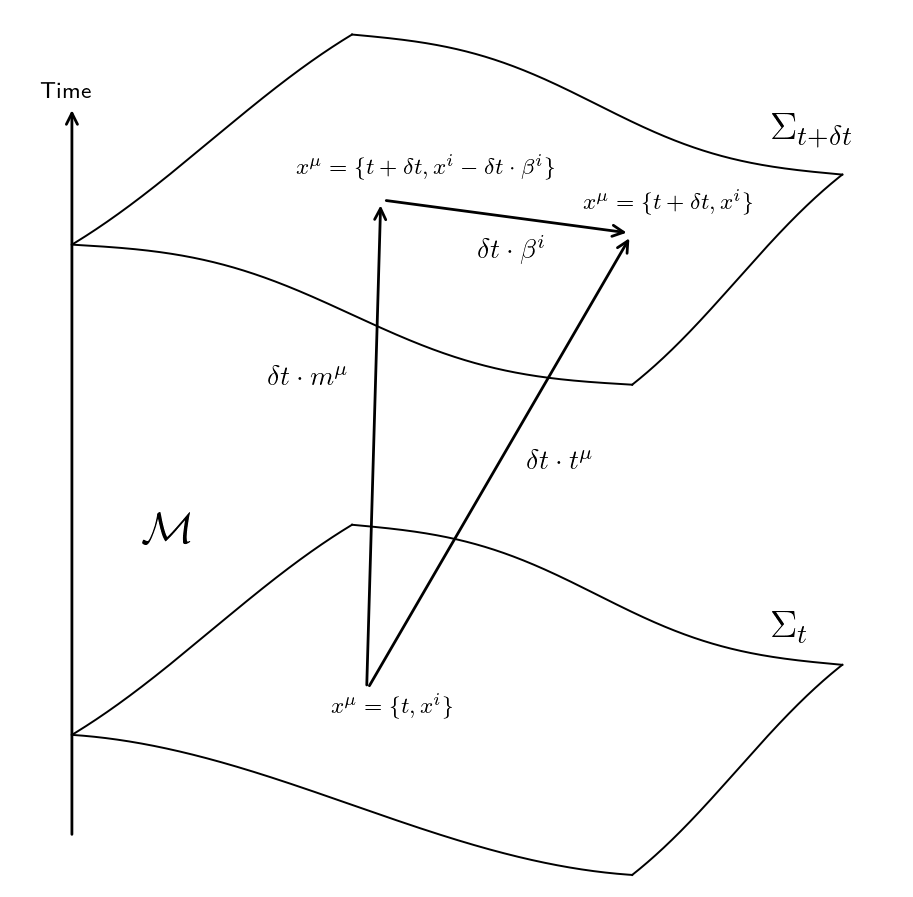
\includegraphics[width=0.65\textwidth]{png/ADM_screeny.png}
    \caption{An illustration of two hypersurfaces $\Sigma_t$ and $\Sigma_{t+\delta}$ and how they are connected by $m^\mu$. As can be seen, integral curves of $t^\mu$ have constant spatial coordinates $x^i$.  }
\end{figure}
There is a large gauge freedom associated with picking coordinates in general relativity; we choose to use a level set of the time coordinate $x^0=t$ to define our foliation hypersurfaces $\Sigma_t$. The other three coordinates $x^i$ for $i\in[1,2,3]$ can be used to span each hypersurface $\Sigma_t$ however we define. It is conventional to split the normal evolution vector $m^\mu$ into time $t^\mu$ and space parts $\beta^\mu$,
\begin{align}
\label{nr:eq:tmu} t^\mu &= \left( 1,0,0,0\right), \\
\label{nr:eq:betamu} \beta^\mu &= \left( 0,\beta^1,\beta^2,\beta^3\right),
\end{align}
such that,
\begin{align}
\label{nr:eq:m1} m^\mu &= t^\mu - \beta^\mu  = (\partial_0)^\mu - \beta^i (\partial_i)^\mu, \\
\label{nr:eq:m2} m^\mu &= \left( 1,-\beta^1,-\beta^2,-\beta^3\right).
\end{align}
We can view $t^\mu$ as the (not necessarily causal) worldline for a simulation gridpoint, hence we would like to evolve our PDEs along $t^\mu$ on a computer. In other words, integral curves of $t^\mu$ must have constant spatial coordinates on $\Sigma_t$. Equation~(\ref{nr:eq:m2}), along with the definitions $\bs{m} = \alpha \bs{n}$ and $\bs{n}^2=-1$, specifies $n^\mu$ and $n_\mu$,
\begin{align}
n^\mu &=  \frac{1}{\alpha}\left( 1,-\beta^1,-\beta^2,-\beta^3\right),\\
n_\mu &= -\alpha\left( 1,0,0,0\right).
\end{align}
The decomposed metric can be calculated, using the property that $\bs{\beta}$ is tangent to $\Sigma_t$ and orthogonal to $\bs{m}$,
\begin{align}
g_{00} &= \bs{g}(\bs{\partial}_0,\bs{\partial}_0) = \bs{g}(\bs{m} + \beta^i \bs{\partial}_i,\bs{m} + \beta^j\bs{\partial}_j) = \bs{g}(\bs{m},\bs{m}) + \beta^i \beta_j \langle \bs{\partial}_i,{\bs{\mathrm{d}}} \bs{x}^j \rangle = -\alpha^2 + \beta^i \beta_i ,\\
 g_{0i} &= \bs{g} (\bs{\partial}_0,\bs{\partial}_i) =  \bs{g}(\bs{m} + \beta^j \bs{\partial}_j, \bs{\partial}_i) =   \beta^j\bs{g}( \bs{\partial}_j, \bs{\partial}_i) = \beta_i,\\
 g_{ij} &= \bs{g}(\bs{\partial}_i,\bs{\partial}_j) = \bs{\gamma}(\bs{\partial}_i,\bs{\partial}_j) = \gamma_{ij}.
 \end{align}
This is commonly called the $3+1$ Arnowitt-Deser-Misner (ADM) metric and $\alpha$, $\beta^i$ are referred to as the lapse and shift vector in this context. The line element and metric are commonly written as,
\begin{align}
\dd s^2 &= -\alpha^2 \dd t^2 + \gamma_{ij}\left[\dd x^i + \beta^i \dd t\right]\left[\dd x^j + \beta^j \dd t\right],\\
 g_{\mu\nu} &= \begin{pmatrix} -\alpha^2 + \beta^i \beta_i & \beta_i \\ \beta_j & \gamma_{ij} \end{pmatrix},\label{nr:eq:admmetric}\\
  g^{\mu\nu} &= \frac{1}{\alpha^2}\begin{pmatrix} -1  & \beta^i \\ \beta^j & \alpha^2\gamma^{ij} - \beta^i \beta^j \end{pmatrix},
 \end{align}
and using Cramer's rule for metric determinant,
\begin{equation} g^{00} = \frac{\det{\gamma_{ij}}}{\det{g_{\mu\nu}}},\end{equation}
we get the important relationship,
\begin{equation} \sqrt{-g} = \alpha \sqrt{\gamma} ,\label{nr:eq:gay}\end{equation}
where $g$ and $\gamma$ are the determinants of $g_{\mu\nu}$ and $\gamma_{ij}$ respectively.

\subsection{ADM Equations} \label{nr:sec:ADM}
Now that we have some coordinates suitable for the spacetime foliation we can find the Arnowitt-Deser-Misner (ADM) evolution equations for $\K_{ij}$ and $\gamma_{ij}$. First we simplify the Lie derivative $\L_t$ along $t^\mu$ using,
\begin{equation}
\L_t \bs{T} = \partial_t \bs{T},
\end{equation}
for any tensor $\bs{T}$ as $\partial_\nu t^\mu=0$. This can be used to expand the Lie derivative along $m^\mu$,
\begin{equation} \L_m = \L_{t} - \L_\beta  = \partial_t - \L_\beta,\end{equation}
and the ADM equations can be written by substituting $\L_m\rightarrow \partial_t - \L_\beta$ in the normal evolution equations in section \ref{nr:sec:einsteindecomp} for $\bs{\K}$ and $\bs{\gamma}$. The ADM equations are,
\begin{align}
\partial_t \K_{ij} &= \L_\beta \K_{ij}  -\D_j\D_i \alpha + \alpha \left[ \R_{ij} + \K\K_{ij} - 2\K^k_i\K_{kj} + 4\pi \left[ \gamma_{ij}\left[ \S-\rho\right]-2\S_{ij}\right]\right],\\
\partial_t \gamma_{ij} &= \L_\beta \gamma_{ij} - 2\alpha\K_{ij}.\end{align}
Unfortunately, these PDEs turn out to be an ill-posed initial value problem with typical gauges \cite{frittelli2000ill}; this means that the time evolution of these equations does not generally depend smoothly on the initial data.


\subsection{BSSN} \label{nr:sec:bssn}
To tackle the ill-posedness of the ADM equations in section \ref{nr:sec:ADM} we
now discuss the Baumgarte-Shapiro-Shibata-Nakamura (BSSN) formalism \cite{Baumgarte:1998te}
The first step in BSSN is to decompose the 3-metric into the conformal metric
$\tilde{\gamma}_{ij}$ and the conformal factor $\chi$,
\begin{align}
\tilde{\gamma}_{ij} &= \chi \gamma_{ij},\\
 \det{\tilde{\gamma}_{ij}} &= \tilde{\gamma} = \chi^3\gamma = 1,
\end{align}
with the above being the convention used in {\sc GRChombo} described in section
\ref{grchombo:sec:grchombo}. Other conventions include factors such as
$\tilde{\gamma}_{ij} = \psi^{-4}\gamma_{ij}$ or $\tilde{\gamma}_{ij} =e^{-\phi}\gamma_{ij}$.
Along with this the extrinsic curvature $\K_{ij}$ is conformally decomposed with
$\chi$ and modified to be trace free,
\begin{equation}
\tilde{A}_{ij} = \chi\left[ \K_{ij}-\frac{1}{3}\K\gamma_{ij}\right],
 \end{equation}
 so that $\tilde{A}_{ij}\gamma^{ij}=0$.
During an evolution the algebraic constraint $\trace{\tilde{A}_{ij}=0}$ (and sometimes
$\tilde{\gamma}=1$) is enforced which avoids the undesirable growth of numerical error
\cite{Gundlach:2006tw,Cao:2011fu}.
As discussed later in
section \ref{nr:sec:gaugeconditions}, the definition of $\chi = \gamma^{-1/3}$
is good for black hole simulations where $\gamma\rightarrow\infty$ but $\chi
\rightarrow 0$. For example the isotropic Schwarzschild metric has,
\begin{align}
\gamma &= \left[ 1+ \frac{M}{2r}\right]^{12},\\
\chi &=\left[ \frac{r}{\frac{M}{2} + r}\right]^4.
\end{align}

The next step is to introduce the conformal connection functions as auxiliary variables,
\begin{align}
 \tilde{\Upsilon}^i_{\,\;jk} &= \frac{1}{2}\tilde{\gamma}^{il}\left[ \partial_j \tilde{\gamma}_{kl} + \partial_k \tilde{\gamma}_{lj} - \partial_l \tilde{\gamma}_{jk}\right] = \Upsilon^i_{\;\,jk} + \left[ \delta^i_j \partial_k + \delta^i_k \partial_j - \gamma^{il}\gamma_{jk}\partial_l\right] \ln \sqrt{\chi},\\
 \tilde{\Upsilon}^i &= \tilde{\gamma}^{jk}\tilde{\Upsilon}^i_{\,\;jk} = -\partial_i \tilde{\gamma}^{ij},
 \end{align}
where $\Gamma^i_{\,\,\,jk}$ are the Christoffel symbols of $\Sigma_t$ as shown
in Eq.~(\ref{nr:eq:3connection});
this reduces the set of vacuum evolution variables to $\{\chi,\tilde{\gamma}_{ij},
\K,\tilde{\A}_{ij},\tilde{\Upsilon}^i \}$. The idea behind introducing the $\tilde{\Upsilon}^i$ is that
their derivatives ($\partial_j\tilde{\Upsilon}^i$) encode second derivatives of the metric
that ruin strong hyperbolicity in the ADM equations; instead these offending terms are
encoded as first derivatives of a new evolution variable and are removed from the principal symbol governing the
hyperbolicity of the equations. It is conventional to use $-\partial_i
\tilde{\gamma}^{ij}$ to evaluate the conformal connection coefficients when they
appear in the RHS of an equation, but $\partial_j \tilde{\Upsilon}^i$ is calculated
by differentiating the evolution variable $\tilde{\Upsilon}^i$.

One final detail, not mentioned in the Z4 and CCZ4 formulations discussed
later, is the addition of multiples of the Hamiltonian and Momentum
constraint equations (in section
\ref{nr:sec:einsteindecomp}) to the evolution equations to change the
characteristic matrix and improve stability. This is not always necessary and
can depend on the gauge used, for more information see \cite{Gundlach:2004jp}.

The BSSN formalism is not the only way to find a well-posed set of evolution
equations for general relativity. Another strongly hyperbolic formalism is the
generalised harmonic gauge \cite{Garfinkle:2001ni,garfinkle2002harmonic,Pretorius:2004jg,Pretorius:2005gq} with,
\begin{equation}\Box x^\mu = H^\mu,\end{equation}
for some functions $H^\mu$.


\subsection{Z4 Formalism}
The Z4 formalism \cite{gundlach2005constraint} generalises the Einstein equation
to include an unphysical field $Z_\mu$, along with damping terms parameterised by
$\kappa_1$, $\kappa_2$,
\begin{equation}
\label{nr:eq:z4einstein} R_{\mu\nu} + \nabla_\mu Z_\nu +
\nabla_\nu Z_\mu - \kappa_1\left[ n_\mu Z_\nu + n_\nu Z_\mu -
[1+\kappa_2]g_{\mu\nu}n^\alpha Z_\alpha\right] = 8\pi G \left[T_{\mu\nu}-
\frac{1}{2}Tg_{\mu\nu} \right].
\end{equation}
Of course regular General Relativity is recovered by setting $Z_\mu=0$. It can
be shown that achieving $Z_\mu=0$ whilst dynamically evolving $Z_\mu$  is
equivalent to solving the constraints. Taking the divergence of
the trace reverse of Eq.~(\ref{nr:eq:z4einstein}),
and noting that both $G_{\mu\nu}$ and $T_{\mu\nu}$ are divergenceless, gives
\begin{equation}
\nabla^\nu \nabla_\nu Z_\mu  + R_{\mu\nu}Z^\nu = -\kappa_1 \nabla^\nu
\left( n_\mu Z_\nu + n_\nu Z_\mu + \kappa_2 g_{\mu\nu} n^\alpha Z_\alpha\right).
\end{equation}
$Z_\mu$ is subjected to a wave equation,
transporting constraint violation off the computational domain. It can be shown
that the system is driven to $Z_\mu =0$ for $k_1>0$ and $k_2>-1$. It is much
cheaper to evolve the variables $Z_\mu$, driven to zero, than to solve four
elliptic PDEs for the constraints $\{\mathcal{H},\M^i\}$ on each timestep.


\subsection{CCZ4} \label{nr:sec:ccz4}
Merging the conformal decomposition of the BSSN formalism with the constraint damping Z4 formalism leads to
Z4c formalism \cite{Bernuzzi:2009ex} and the conformal covariant Z4 (CCZ4) formalism.
The purpose of this is to get a formalism combining the strong hyperbolicity
of the BSSN equations and the constraint damping effects of the Z4 system.
In this thesis
we will use the CCZ4 formalism which employs the additional modifications,
\begin{align} \Theta &= -n\cdot Z  = -\alpha Z^0,\\
\hat{\Upsilon}^i &= \tilde{\Upsilon}^i + \frac{2\gamma^{ij}Z_j}{\chi},\end{align}
leaving us with the following set of vacuum evolution variables
$\{\chi, \tilde{\gamma}_{ij},\K,\tilde{\A}_{ij},\hat{\Upsilon}^i,\Theta \}$.
The evolution equations can now
be found in the CCZ4 scheme by applying a 3+1 decomposition to the Z4 modified
Einstein equation~(\ref{nr:eq:z4einstein}) and proceding as in the BSSN formalism.
To illustrate this, we derive the equation of motion for $\chi$ in the CCZ4 formalism.
Using Eqs.~(\ref{intro:eq:mdmmdm}) and (\ref{nr:eq:Lmgamma}) with $\chi^{-3}=\gamma$
we obtain,
\begin{align}
\L_m {\gamma} = \gamma \gamma^{ij} \L_m \gamma_{ij} = -2 \gamma \alpha \gamma^{ij} \K_{ij} = -2\gamma \alpha \K.
\end{align}
This can be used to simplify the Lie derivative of $\chi$,
\begin{align}
\L_m \chi &= \L_{\partial_t}\chi - \L_\beta \chi,\\
 &= (\partial_t)^i \partial_i \chi + \omega \chi \partial_i (\partial_t)^i - \beta^i \partial_i \chi - \omega \chi \partial_i \beta^i ,\\
 &= \partial_t \chi - \beta^i \partial_i \chi +\frac{2}{3} \chi\partial_i \beta^i ,\\
\L_m \chi &= \L_m \gamma^{-\frac{1}{3}}  ,\\
&=-\frac{1}{3}\gamma^{-\frac{4}{3}}\L_m \gamma  ,\\
&=\frac{2}{3}\gamma^{-\frac{1}{3}} \alpha \K ,\\
&=\frac{2}{3}\chi \alpha \K ,
\end{align}
where Eq.~(\ref{intro:eq:Ltensordensity2}) has been used with $\bs{\mathcal{T}}=\chi$ as $\chi$ is a scalar density of weight $\omega=-2/3$. Re-arranging gives the equation of motion for $\chi$,
\begin{equation}
\partial_t \chi =  \beta^i \partial_i \chi + \frac{2\chi}{3} \left[\alpha \K - \partial_i \beta^i \right].
\end{equation}
A similar process returns the remaining CCZ4 equations but care should be taken to include the Z4 terms ($\Theta,\hat{\Upsilon}^i$) where they are needed. The complete list of CCZ4 equations used in simulations with {\sc GRChombo} (section \ref{grchombo:sec:grchombo}) are given below:
\begin{align} \partial_t \chi &=  \beta^i \partial_i \chi + \frac{2\chi}{3} \left[\alpha \K - \partial_i \beta^i \right],\\
\partial_t\tilde{\gamma}_{ij} &=  \beta^k\partial_k\tilde{\gamma}_{ij}  + \tilde{\gamma}_{kj}\partial_i \beta^k + \tilde{\gamma}_{ik}\partial_j\beta^k - \frac{2}{3}\tilde{\gamma}_{ij} \partial_k \beta^k - 2\alpha\tilde{\A}_{ij},\\
\partial_t\K &=  \beta^k\partial_k\K + \alpha\left[ \R + 2\bs{\D}\cdot \bs{Z} + \K\left[ \K-2\Theta\right]\right] - 3\alpha \kappa_1\left[ 1+\kappa_2\right]\Theta \nonumber\\
&-\chi\tilde{\gamma}^{kl}\D_k\D_l\alpha + 4\pi G\alpha\left[ \S - 3\rho\right], \\
\partial_t\tilde{\A}_{ij} &=  \beta^k \partial_k \tilde{\A}_{ij}+\chi\left[\alpha\left[\R_{ij} + 2\D_{(i}Z_{j)}-8\pi G \S_{ij} \right] -\D_i\D_j\alpha \right]^{TF}\nonumber\\
& +\tilde{\A}_{ij}\left[ \alpha\left[ \K-2\Theta\right]-\frac{2}{3}\K^2\right] + 2\tilde{\A}_{k(i}\partial_{j)}\beta^k -2\alpha\tilde{\gamma}^{kl}\tilde{\A}_{ik}\tilde{\A}_{lj},\\
\partial_t\Theta &= \beta^k\partial_k \Theta + \frac{1}{2}\alpha\left[ \R + 2\bs{\D}\cdot \bs{Z} - \tilde{\A}_{kl} \tilde{\A}^{kl} + \frac{2}{3}\K^2 - 2\Theta\K\right] -\kappa_1\alpha\Theta\left[ 2+\kappa_2\right] - Z^k\partial_k\alpha - 8\pi G \alpha \rho, \\
\partial_t\hat{\Upsilon}^i &=  \beta^k \partial_k \hat{\Upsilon}^i + \frac{2}{3}\left[ \partial_k \beta^k \left[ \tilde{\Upsilon}^i+2\kappa_3 \frac{Z^{i}}{\chi}\right]-2\alpha\K\frac{Z^j}{\chi}\right]-2\alpha\kappa_1\frac{Z^i}{\chi}\nonumber \\
& + 2\tilde{\gamma}^{ij}\left[ \alpha\partial_j\Theta -\Theta \partial_j\alpha \right] -2\tilde{\A}^{ij}\partial_j\alpha - \alpha\left[ \frac{4}{3}\tilde{\gamma}^{ij}\partial_j\K + 3\tilde{\A}^{ij}\frac{\partial_j \chi}{\chi}\right]\nonumber\\
& -\left[ \tilde{\Upsilon}^j + 2\kappa_3 \frac{Z^j}{\chi}\right]\partial_j \beta^i + 2\alpha \tilde{\Upsilon}^i_{\,\,\,jk}\tilde{\A}^{jk} + \tilde{\gamma}^{jk}\partial_j\partial_k \beta^i + \frac{1}{3} \tilde{\gamma}^{ij}\partial_k \partial_j \beta^k - 16\pi G \alpha \tilde{\gamma}^{ij}\S_j, \\
\partial_t \vp &= \beta^k\partial_k \vp - \alpha\Pi ,\label{nr:eq:ccz4kg1}.\end{align}
In the CCZ4 equations there is an additional parameter $\kappa_3$ premultiplying terms in the evolution of $\hat{\Upsilon}^i$ which experimentally were found to lead to instabilities in black hole simulations \cite{PhysRevD.85.064040}; setting $\kappa_3<1$ stabilises the simulation but at the cost of covariance. Later on it was realised that setting $\kappa_3=1$ and $\alpha\kappa_1\rightarrow\kappa_1$ retains covariance as well as numerical stability \cite{Alic:2013xsa}; in this work $\kappa_1=0.1$, $\kappa_2=0$ and $\kappa_3=1$ is used. Notably the pair of variables $\R_{ij} + \D_{(i}Z_{j)}$, and its traced version
$\R + \bs{\D}\cdot \bs{Z}$, always appear together; separately they would ruin
strong hyperbolicity but together they do not.


The CCZ4 scheme proves several benefits.
\begin{itemize}
\item Any initial data that does not satisfy the constraints will generally not do so during evolution when using the BSSN formalism either. Given that superposition of solutions in GR does not generally give a new solution, but does approximate one for separated compact objects, all the simulated binaries considered in this work will have non constraint satisfying initial data.
\item Constraint satisfying initial data can also develop constraint violation over time; one reason being that finite resolution imposes some small deviation from the continuum solution. More importantly, the use of adaptive mesh refinement (discussed in section \ref{grchombo:sec:grchombo}) introduces interpolation errors into the simulation at the boundary of the different grid resolution levels. The use of the CCZ4 scheme can also help to reduce the constraint violation generated in this way.
\item Sommerfeld boundary conditions (discussed in section \ref{grchombo:sec:sommerfeld}) used are inexact in GR and will introduce errors at the outer boundary that ruin constraint satisfaction and in the worst case scenario cause a simulation to crash. Again, the CCZ4 scheme can be used to help combat this.
\end{itemize}
In all the cases above, the CCZ4 system forces the evolution towards constraint satisfaction, despite the numerical errors and approximations. There is a caveat, even if a simulation satisfies the constraints, there is no guarantee it is the desired solution to Einstein's equation. Additionally, the damping is more efficient for small amplitude and high frequency errors.



\subsection{Gauge Conditions}\label{nr:sec:gaugeconditions}

The lapse $\alpha$ and shift $\beta^i$ are freely specifiable on a hypersurface
$\Sigma_t$ being gauge variables, however they must be chosen carefully along with
a suitable initial Cauchy surface $\Sigma_{t_0}$ and initial data. $\Sigma_{t_0}$
should be a smooth non-intersecting Cauchy surface as described in section
\ref{nr:sec:foliation} and contain smooth initial data. It is also wise to avoid
singularities (both coordinate and physical) on this surface. As an example,
consider the simulation of a single Schwarzschild black hole.
Figure~\ref{nr:fig:eddington-finkelstein} (left) shows how an initial data
surface could extend to the singularity if polar-areal coordinates are used.
Figure~\ref{nr:fig:eddington-finkelstein} also shows how the physical singularity
is avoided when using isotropic coordinates. In this work the isotropic gauge is
used; not only does this provide an initial Cauchy surface free of physical
singularities but also allows for trivial swapping between spherical polar and
Cartesian (used in simulations) coordinates. However, for a poor choice of
lapse function, even a well chosen $\Sigma_{t_0}$ can advance to the physical
singularity in finite simulation time.  For a comprehensive introduction to gauge
conditions the reader is directed to
\cite{baumgarte_shapiro_2010,alcubierre2008introduction,gourgoulhon20073+}.

%   \begin{figure}[h]
%   \caption{Penrose Diagrams, $\Sigma_{t_0}$ dashed, Left: Ingoing Eddington-Finkelstein Coordinates, Right: Isotropic Coordinates.}
%   \centering
%   \subfloat{\includegraphics[width=0.43\textwidth]{schwarzschild2.png}\label{boson:fig:f1}} \label{nr:fig:eddington-finkelstein}
%   \hfill
%   \subfloat{\includegraphics[width=0.5\textwidth]{schwarzschild.png}\label{boson:fig:f2}} \label{nr:fig:isotropic}
% \end{figure}

  \begin{figure}[h]
  \caption{Penrose Diagram of the maximally extended Schwarzschild spacetime; the top (future) squiggle represents the spacelike black hole singulary and the bottom (past) squiggle represents the white hole singularity. In the right hand diagram, the straight dashed line labelled by $\Sigma_{\rm iso}$ represent the initial hypersurface $\Sigma_{t_0}$ for $t=0$ in isotropic coordinates. In the left hand diagram, the dashed line labelled by $\Sigma_{\rm pa}$ represent the initial hypersurface $\Sigma_{t_0}$ for $t=0$ in polar-areal coordinates. Notably $\Sigma_{\rm pa}$ initially touches the physical singularity whereas $\Sigma_{t_0}$ does not; additionally $\Sigma_{\rm pa}$ is not a Cauchy surface as there exist causal curves which can intersect it multiple times.}
  \centering
  \subfloat{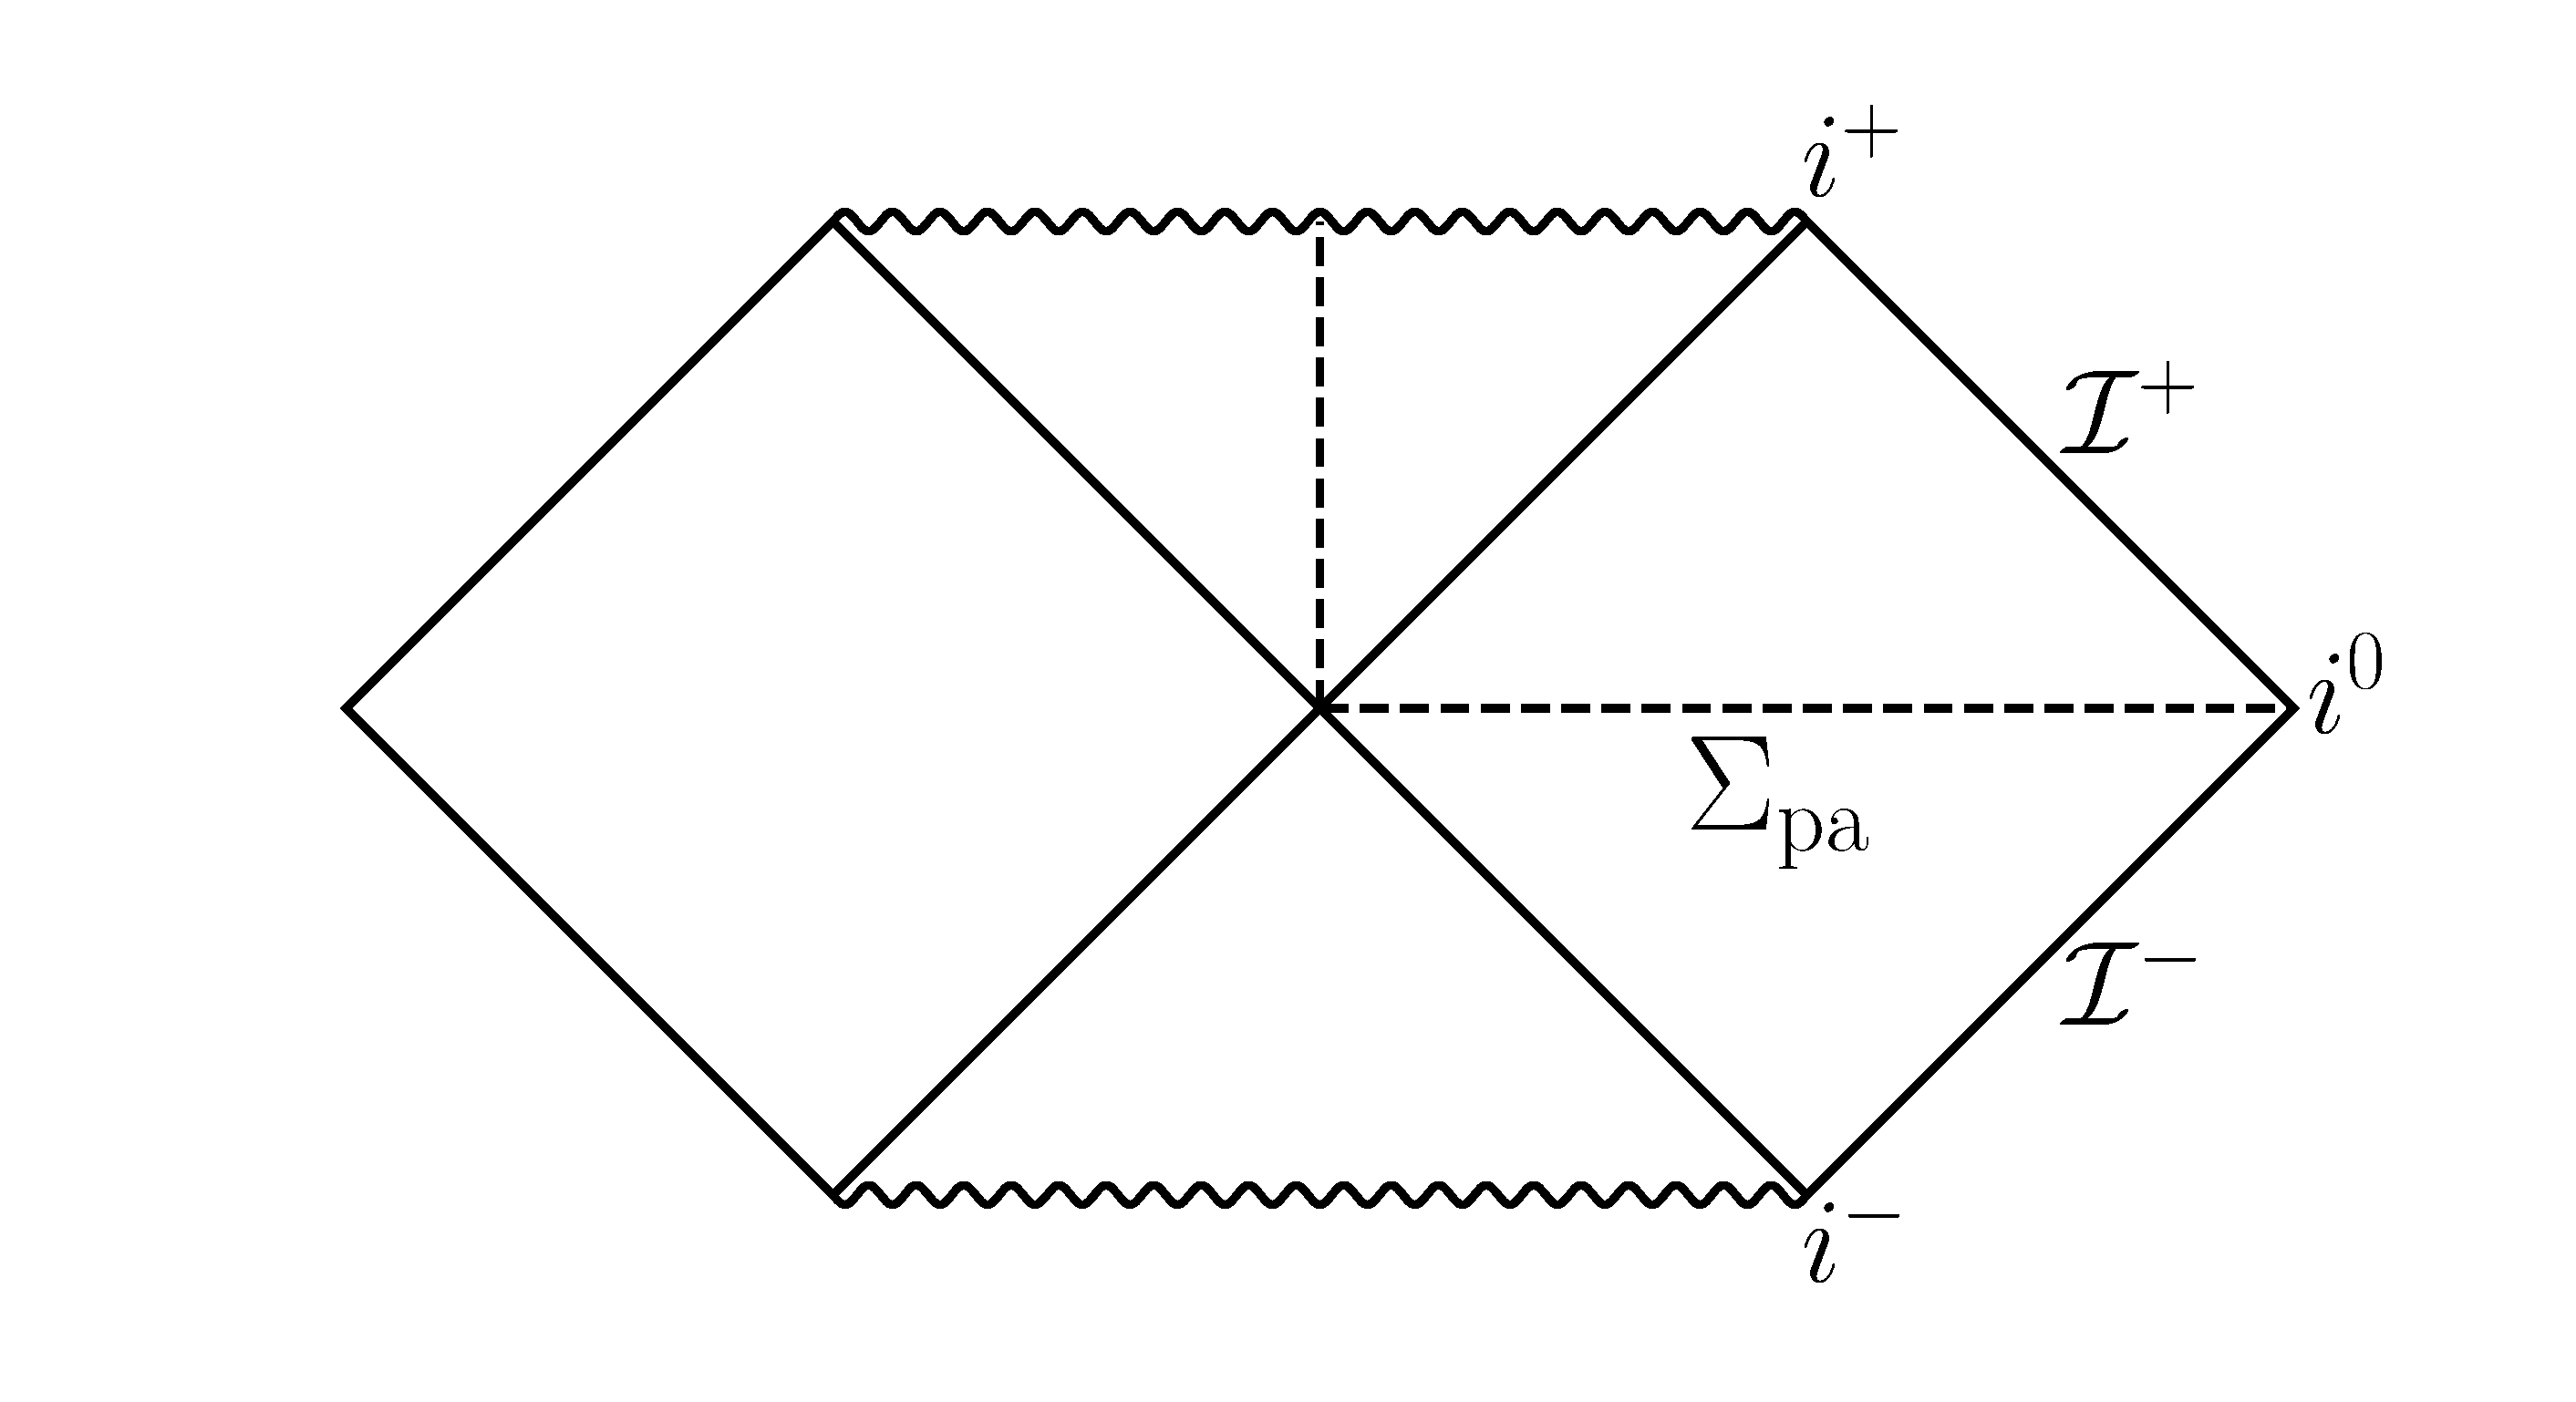
\includegraphics[width=0.50\textwidth]{png/penrose_sc.pdf}} \hfill
  \subfloat{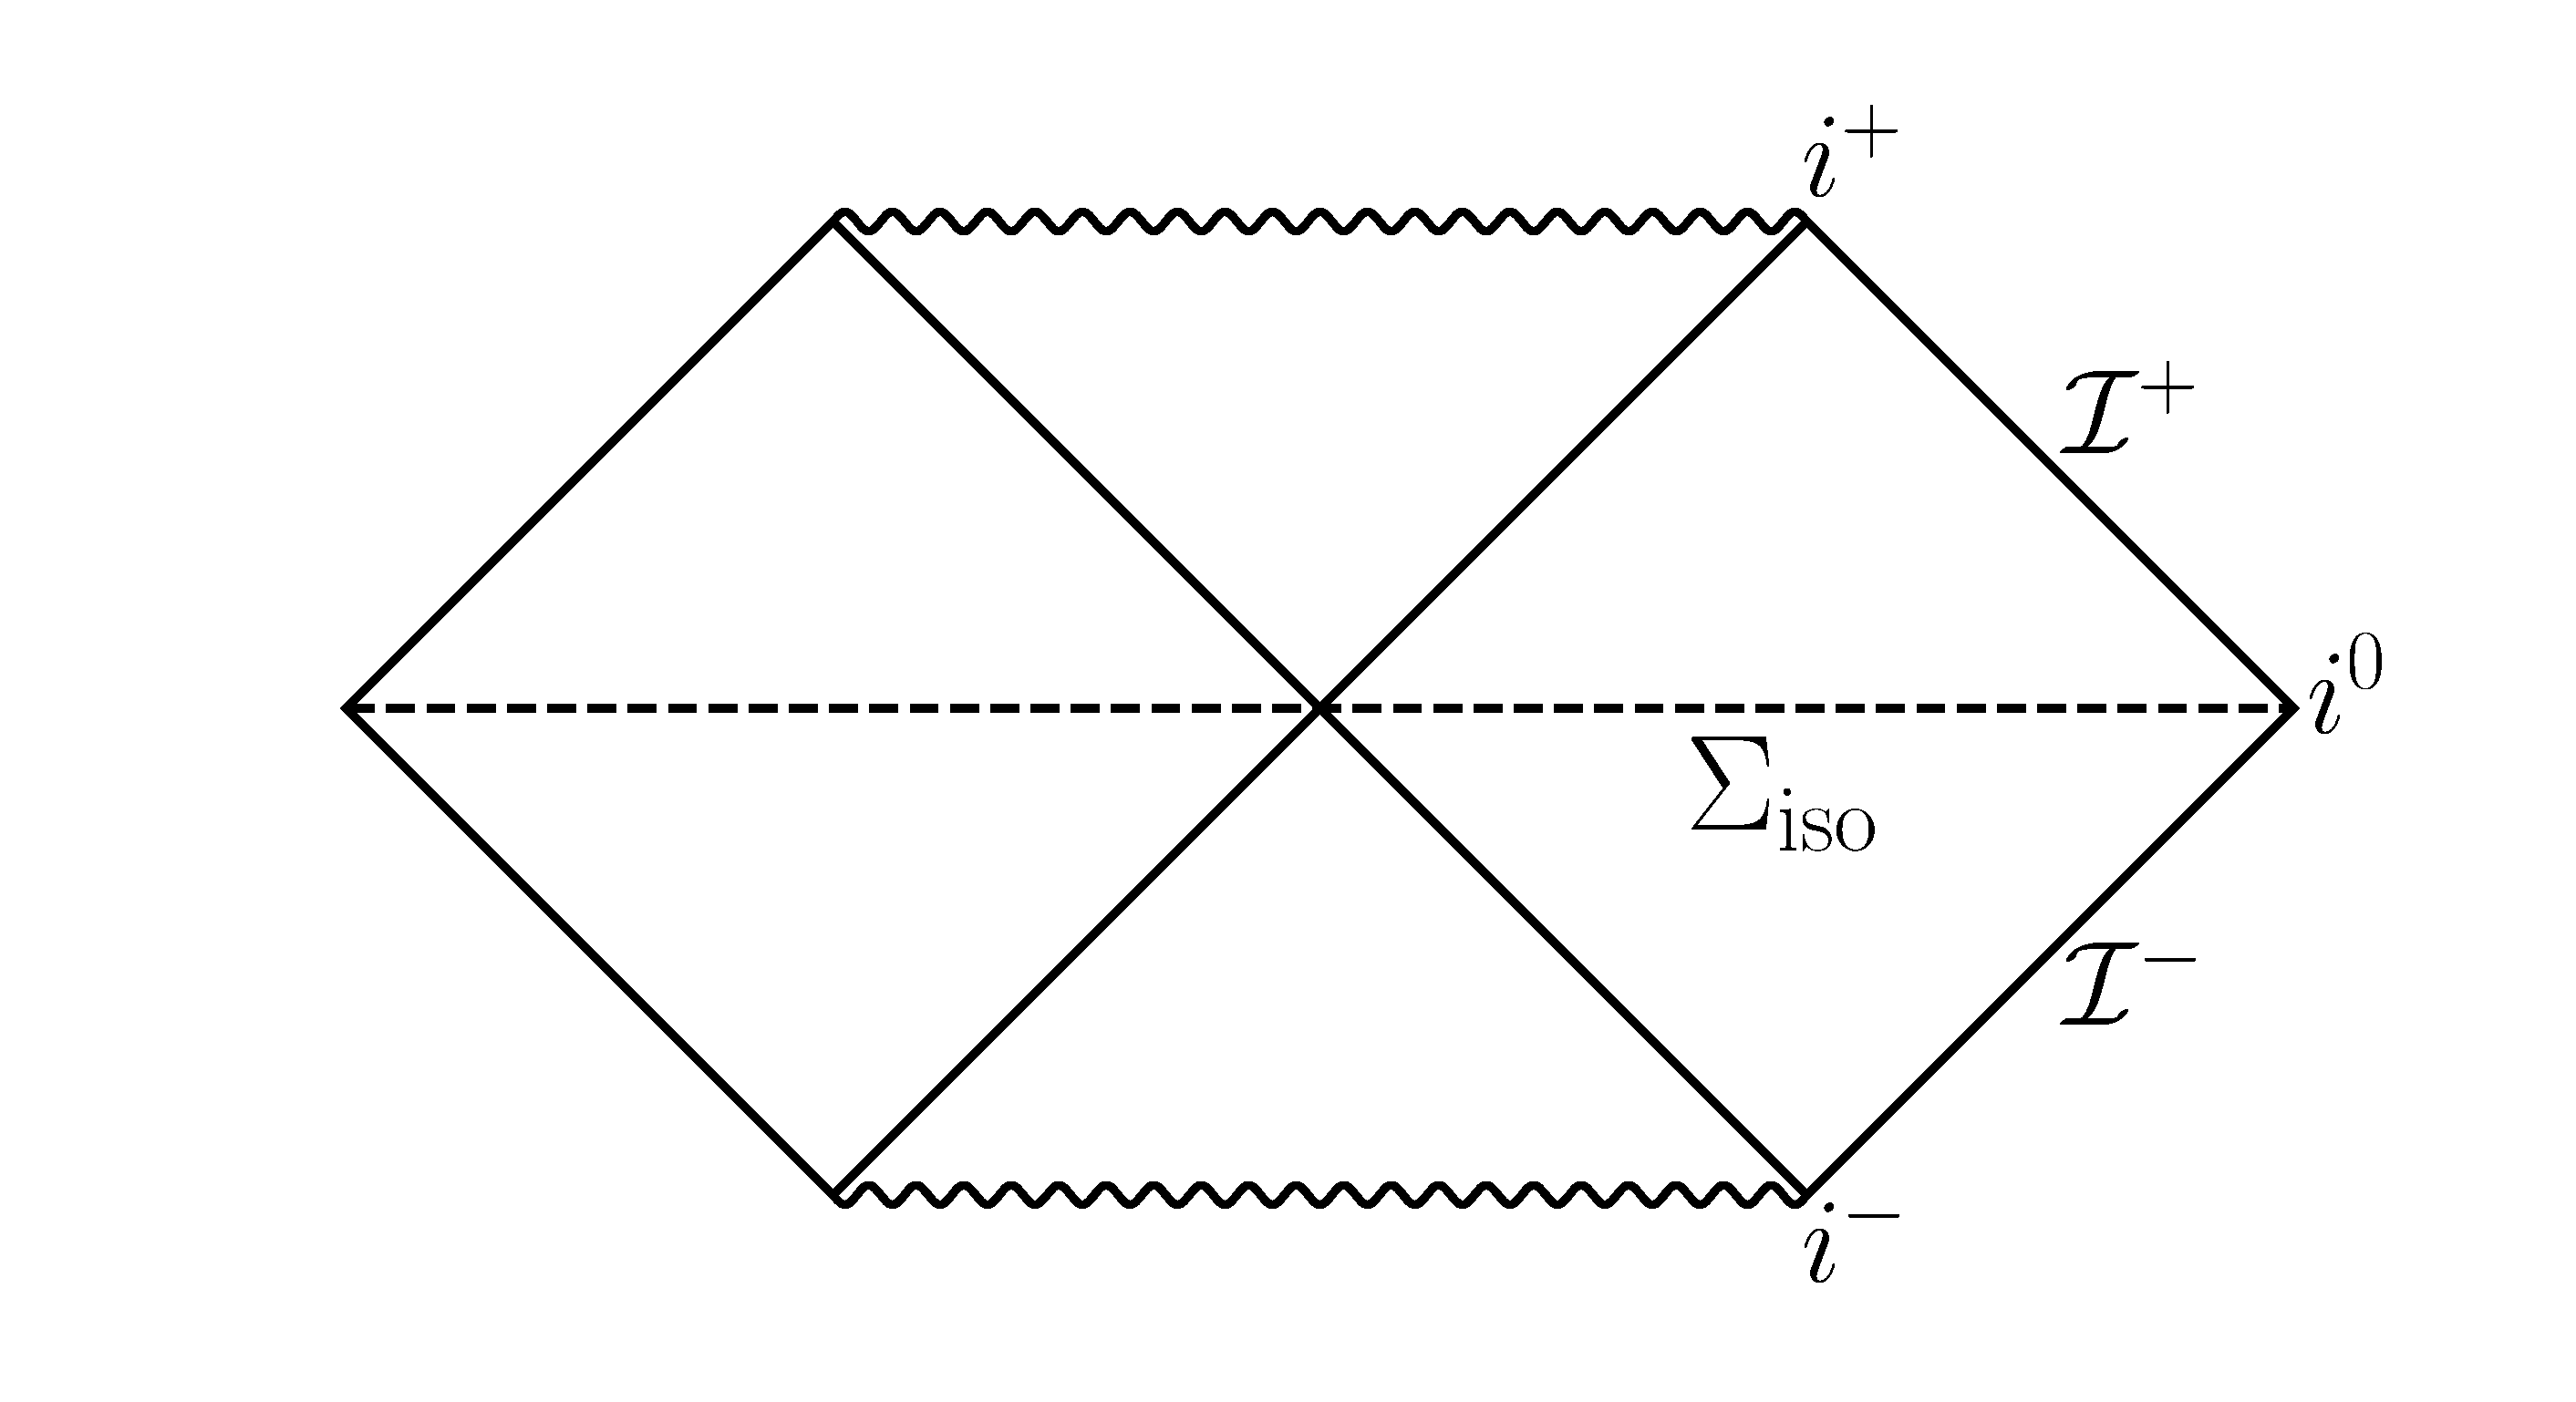
\includegraphics[width=0.50\textwidth]{png/penrose_iso.pdf}}
  \label{nr:fig:eddington-finkelstein}\label{nr:fig:isotropic}\label{boson:fig:f1}
\end{figure}

\subsubsection{Lapse Slicing Conditions}

The simplest lapse choice would be to enforce $\alpha=1$, called geodesic slicing, with the hypersurface following integral curves of $n^\mu$; given that geodesics can converge this can lead to hypersurface self-intersection which breaks the definition of a Cauchy surface and the simulation will likely fail. Another problem is that a black hole singularity can be reached in finite simulation time.

An alternative slicing condition is the maximal slicing condition which keeps the volume element $\sqrt{-g}$ constant along geodesics. This means as $\gamma\rightarrow\infty$ nearing a singularity $\alpha\rightarrow0$ from Eq.~(\ref{nr:eq:gay}), causing the hypersurface to advance more slowly before a singularity is reached as demonstrated in Fig.~(\ref{nr:fig:singularity_avoiding}). This property is called singularity avoiding and is crucial for numerical stability unless using excision\footnote{Excision is the practice of cutting singularities out of the computational domain while supplying suitable boundary conditions about the excised region}. Maximal slicing can be implemented by forcing $\mathcal{K} = \partial_t \K = 0\,\forall \,t$ which requires a slow elliptic solve for $\alpha$ at each timestep. Instead of performing this slow elliptic solve, $\alpha$ is promoted to an evolution variable and is evolved along with every other simulation variable. To do this we can pick an algebraic slicing condition of the Bona-Masso type,
\begin{equation}\L_m \alpha = \partial_t \alpha - \beta^i \partial_i \alpha = -\alpha^2 f(\alpha)\K. \end{equation}
Using this with $f = 2\alpha^{-1}$ gives,
\begin{equation}\L_m \alpha = \partial_t \alpha - \beta^i \partial_i \alpha = -2\alpha \K, \label{nr:eq:1pluslog} \end{equation}
which is called 1+log slicing; this is very common in Numerical Relativity codes. In practice 1+log slicing is strongly singularity avoiding reaching $\alpha=0$ before the singularity. This is modified in the CCZ4 scheme to,
\begin{equation}\partial_t \alpha = -2\alpha\left[ \K-2\Theta\right] + \beta^i \partial_i \alpha.\end{equation}
Using Gaussian normal coordinates $\beta^i=0$ and provided $\Theta=0$, the 1+log slicing condition reduces to,
\begin{equation} \alpha = 1+ \ln \gamma,\end{equation}
giving the slicing condition it's name \cite{alcubierre2008introduction}.

\begin{figure}[h!]
    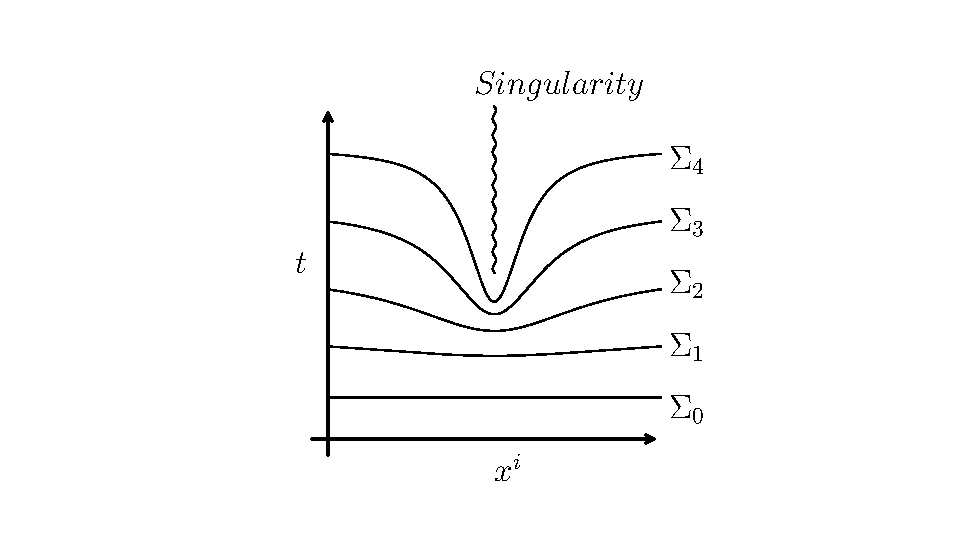
\includegraphics[width=0.9\textwidth]{png/slicing.pdf}
      \caption{Diagram showing the time evolution of a hypersurface using a singularity avoiding slicing condition. The vertical squiggled line represents a physical singularity that is formed at some point in spacetime, potentially from the collapse of matter to a black hole.} \label{nr:fig:singularity_avoiding}
\end{figure}


\subsubsection{Shift Conditions}

The simplest choice for the shift vector would be $\beta^i=0$ but this can cause great stretching and shearing of integral curves of $m^\mu$ in the neighbourhood of a singularity as in Fig.~(\ref{nr:fig:singularity_avoiding}); the effect of this is that neighbouring gridpoints may have large differences in field values leading to inaccurate and unstable evolutions.

 Another negative side effect is that the computational domain can fall inside an event horizon in black hole simulations. To counteract this we want to employ a shift vector that minimises hypersurface shear $\sigma_{ij}$ which can be defined as \cite{smarr1978kinematical},
\begin{equation} \sigma_{ij}:= \perp^\mu_i \perp^\nu_j \left[\nabla_{(\mu} n_{\nu)}-\frac{1}{3}\gamma^{ab}\nabla_{(a} n_{b)} \gamma_{\mu\nu}\right], \end{equation}
where $\sigma_{ij}$ is tracefree corresponding to shearing rather than inflation or expansion. Minimising the total shear $\Sigma$,
\begin{equation} \Sigma = \int \sigma_{ij}\sigma^{ij}\sqrt{\gamma}\,\dd x^3,\end{equation}
with respect to $\beta^i$ leads to an elliptic PDE to be solved for each $\beta^i$ at each time step that minimises shear,
\begin{equation} \delta \Sigma = 0 \rightarrow \D_i\sigma^{ij}=0.\end{equation}
This is known as the minimal distortion shift condition. Promoting the $\beta^i$ to evolution variables is computationally cheaper than solving a set of PDEs at each time step. A very common choice is to promote the elliptic PDE for $\beta^i$ into a hyperbolic equation via introducing a $\partial_t^2\beta^i$ term and an artificial damping term parameterised by $\eta$. This becomes a damped wave equation and is supposed to transport away any part of $\beta^i$ which does not satisfy $\D_i \sigma^{ij}=0$. This works well with Sommerfeld (outgoing wave) boundary conditions given in section \ref{grchombo:sec:sommerfeld}. The standard Gamma driver shift condition is,
\begin{align}
\partial_t \beta^i &= FB^i,\label{nr:eq:gammadriver1}\\
 \partial_t B^i &= \partial_t \tilde{\Gamma}^i - \eta B^i,\label{nr:eq:gammadriver2}\end{align}
where $F=3/4$ and $\eta=1$ are used throughout this work.

\subsubsection{Moving Puncture Gauge}
The moving puncture gauge (MPG) is the combination of the 1+log slicing lapse condition
in Eq.~(\ref{nr:eq:1pluslog}) and the Gamma driver shift condition in
Eqs.~(\ref{nr:eq:gammadriver1}) and (\ref{nr:eq:gammadriver2}). In 2006, the
moving puncture gauge allowed for the first successful simulation of a black hole
binary \cite{PhysRevLett.96.111101} in the BSSN
formalism\footnote{It should be noted that a black-hole binary had been sucessfully
simulated before by \cite{Bruegmann:2003aw} in 2003 with co-rotating coordinates
and \cite{Pretorius:2005gq} in 2005 using the generalised harmonic gauge.} without
the use of excision. In 2012 the first simulations of black-hole binaries
using constraint damping schemes (in the MPG) such as CCZ4 \cite{alic2012conformal}
and Z4c \cite{Hilditch:2012fp} were achieved.
Although $\chi\rightarrow 0$, or $\gamma \rightarrow \infty$,
at the centre of a black hole, as long as a minimum value for $\chi$
(such as $\chi=10^{-4}$) is enforced a simulation can run. Even though it is
unphysical to modify a physical variable, the success of the MPG is often attributed
to the causal shielding\footnote{Errors that propagate at (or below) light speed
will be trapped by the event horizon. } provided by the
event horizon. Additionally, any extremely sharp field configurations produced will
be partially suppressed by a numerical dissipation scheme.

Not only does the MPG safeguard the divergence of fields at the puncture, but it allows the puncture to move; hence the name {\it moving} puncture gauge. Near the puncture, the lapse $\alpha$ becomes vanishingly small and the 1+log slicing condition in Eq.~(\ref{nr:eq:1pluslog}) becomes,
\begin{equation}
\partial_t \alpha = \beta^i \partial_i \alpha, \label{nr:eq:betavel}
\end{equation}
which causes the puncture to move. Assigning spatial coordinates $x^i_{\rm punc}(t)$ to the puncture, we know that
\begin{align}
\alpha(x^i_{\rm punc}) &= 0,\\
\frac{\dd}{\dd t} \alpha(x^i_{\rm punc})  &= \frac{\partial}{\partial t}\alpha + \left(\frac{\partial x^i}{\partial t}\Bigg|_{x^i=x^i_{\rm punc}}\right)\frac{\partial}{\partial x^i} \alpha =0,
\end{align}
which can be compared to Eq.~(\ref{nr:eq:betavel}) to show that
\begin{equation}
\beta^i = -\frac{\partial }{\partial t}x^i_{\rm punc}\,.
\end{equation}
This shows that the puncture must move along integral curves of $-\beta^i$.


%







\section{Numerical Methods} \label{grchombo:sec:numericalmethods}

\subsection{Introduction to Numerical Methods}

In classical physics it is common for a system to be described by the solution of a differential equation (or a set of differential equations) subjected to suitable boundary conditions. There exist many cases, where the system is sufficiently simple, in which the differential equation(s) can be solved analytically; some well known examples include Newton's equation of gravity for orbits, the Schrödinger equation for certain potentials (such as the infinite square well and the quadratic potential) and Maxwell's equations for electromagnetic fields.

In four space-time dimensions, general relativity is a set of ten coupled non-linear differential equations. The complexity of general relativity means that analytic solutions are usually restricted to spacetimes with symmetries or simplifying assumptions. Some common examples are single eternal black hole solutions, cosmological solutions for a uniform universe and the flat Minkowski space. In the case of colliding compact objects (such as black holes, neutron stars or boson stars) there is no analytic solution and numerical methods are the only way to solve the differential equations governing the system.

The rest of section \ref{grchombo:sec:numericalmethods} introduces the reader to
the basic concepts in numerical methods such as discretisation, boundary conditions
and time evolution. Section \ref{grchombo:sec:grchombo} describes {\sc GRChombo},
the numerical relativity code used throughout this thesis, and is loosely based on
the collaboration paper \cite{Andrade2021}. From section \ref{grchombo:sec:units}
onward, the rest of the chapter covers the numerical creation of known boson star
initial data for use in simulations; the solution is found directly in the isotropic gauge
rather than the polar areal gauge used in the literature \cite{Schunck:2003kk,Liebling:2012fv}.
Finally numerical simulations of a head-on and grazing boson star collision are
presented in Section~\ref{grchombo:sec:bscollisions}.

\subsection{Numerical Discretisation of Spacetime} \label{grchombo:sec:numericaldisc}

There are many ways to time evolve a field theory on a spatial surface. Some popular numerical methods include spectral methods, finite element models and finite volume methods. The method used throughout this work is the finite difference framework. This models a continuous spacetime with a discrete lattice of points; usually this lattice is cubic or cuboidal. A field $\phi(x^\mu)$ on a manifold $\M$ is expressed as a set of discrete values $\phi^n_{ijk}$, for integer $\{n,i,j,k\}$, on a set of discrete lattice points with coordinates $(x^n_{ijk})^\mu$. In uniform Cartesian coordinates $(x^n_{ijk})^\mu= \{n \Delta t, i \Delta x, j \Delta y, k \Delta z \}$ where $\Delta t$, $\Delta x$, $\Delta y$ and $\Delta z$ represent the grid spacing. In the limit that the grid spacing tends to zero, the lattice and discretised fields should converge to the continuum solution. For a detailed introduction to numerical methods the reader is directed to \cite{Press1992}.

To calculate gradients on a lattice, we can consider a two dimensional manifold spanned by coordinates $\{t,x\}$. We can no longer employ the traditional definition of $\dd f / \dd x$,
\begin{equation}
\frac{\dd f}{\dd x} := \lim_{\delta x \rightarrow 0} \left( \frac{f(x+\delta x)-f(x)}{\delta x} \right),
\end{equation}
as there no longer exist two points $x$ and $x+\delta x$ that are infinitesimally close to each other. Derivatives are now approximately calculated by comparing gridpoints a finite distance from each other. To elucidate this idea, a formula for the second derivative is calculated. First we pick five lattice points, equally spaced by $\Delta x$, with coordinates $\{x_{-2},x_{-1},x_{0},x_{1},x_{2}\}$, and writing $f(x_i) = f_i$. Then using the well known formula for the Taylor expansion of a function about a point $x_0$,
\begin{equation}
f(x) = f(x_0) + (x-x_0) f'(x_0) + \frac{(x-x_0)^2}{2!}f''(x_0) + \frac{(x-x_0)^3}{3!}f'''(x_0) + ... \,, \label{grchombo:eq:taylor}
\end{equation}
 we can write,
\begin{align}
f_{2} &\approx f_0 + 2\Delta x f'_0 + 2 (\Delta x)^2 f''_0 + \frac{4}{3}(\Delta x)^3 f'''_0+ \frac{2}{3} (\Delta x)^4 f''''_0, \\
f_{1} &\approx f_0 + \Delta x f'_0 + \frac{1}{2}(\Delta x)^2f''_0 + \frac{1}{6}(\Delta x)^3f'''_0 + \frac{1}{24}(\Delta x)^4f''''_0,\\
f_0 &\approx f_0 , \\
f_{-1} &\approx f_0 - \Delta x f'_0 + \frac{1}{2}(\Delta x)^2f''_0 - \frac{1}{6}(\Delta x)^3f'''_0 + \frac{1}{24}(\Delta x)^4f''''_0,\\
f_{-2} &\approx f_0 - 2\Delta x f'_0 + 2 (\Delta x)^2 f''_0 - \frac{4}{3}(\Delta x)^3 f'''_0+ \frac{2}{3} (\Delta x)^4 f''''_0,
\end{align}
where the Taylor expansions are truncated at terms of order $(\Delta x)^4$. The equations above can be inverted to give,
\begin{equation}
\frac{\dd^2 f}{\dd x^2}\Bigg|_{x_0}:=f''_0 = \frac{-f_2 + 16 f_1 - 30 f_0 + 16 f_{-1} - f_{-2} }{12 (\Delta x)^2}+\mathcal{O}(\Delta x^4). \label{grchombo:eq:d2fdx2}
\end{equation}
An approximation for the second derivative using a discrete sum of neighbouring points, also called a stencil, has been obtained. Adding terms of order $(\Delta x)^5$ in the Taylor expansion for $f_i$ would not affect the result as the pairs of terms $\{f_2,f_{-2}\}$ and $\{f_1,f_{-1}\}$ appear in equal amounts; therefore Eq.~(\ref{grchombo:eq:d2fdx2}) is correct up to a Taylor expansion of order $(\Delta x)^6$. Given that $f''_0$ appears with a $(\Delta x)^2$ and Eq.~(\ref{grchombo:eq:d2fdx2}) is correct until terms of order $(\Delta x)^6$, then the expression is accurate up to fourth order. Any other derivative to any order accuracy (in any dimension) can be calculated in a similar fashion. In the limit that the grid spacing $\Delta x \rightarrow 0$ the approximations for the derivatives approach the exact continuum limit while higher order accurate stencils approach the continuum limit more quickly.


\subsection{Boundary Conditions} \label{grchombo:sec:bc}
Another artefact of evolving field equations over a volume on a computer is that the volume must have finite size; a computer does not have infinite memory to store an infinite amount of gridpoints. The usual way to deal with this problem is to enforce an algebraic condition on the fields on a surface surrounding the region of interest. Alternatively, an infinite volume can be modelled if coordinates are used which compactify the volume to some finite region, this corresponds to the grid spacing $\Delta x$ diverging or resolution becoming infinitely low towards the boundary.

Common boundary conditions include Dirichlet (fixed value), Von-Neumann (fixed derivative) or some mix of these conditions. It is common to re-categorise boundary conditions into sub-categories with informative names such as reflective, periodic or symmetric.

As an example in one spatial dimension, symmetric boundary conditions for a field $\phi$ about a point $x_n$ could be implemented by creating extra {\it ghost cells} beyond the desired simulation domain with coordinates $\{x_{n+1},x_{n+2},x_{n+3},...\}$ and setting,
\begin{align}
\phi_{n+1} = \pm\phi_{n-1}, \quad \phi_{n+2} = \pm\phi_{n-2}, \quad \phi_{n+3} = \pm\phi_{n-3}, \quad ... \, ,
\end{align}
where the $+$ or $-$ sign is taken for even or odd parity variables and $\phi_i = \phi(x_i) = \phi(i*\Delta x)$. These extra ghost cells allow the calculation of derivatives at $x_n$ using stencils, as shown in section \ref{grchombo:sec:numericaldisc}; without these ghost cells the stencil would not be able to access points $x_{m}$ where $m>n$. The number of ghost cells should be chosen to be the minimum required to allow the calculation of derivative stencils at each point in the simulation domain. The desired location of the boundary condition does not have to coincide with a gridpoint. As an example, modifying the symmetric boundary condition to be centred on $x_n + \Delta x /2$ instead results in,
\begin{align}
\phi_{n+1} = \pm\phi_{n}, \quad \phi_{n+2} = \pm\phi_{n-1}, \quad \phi_{n+3} = \pm\phi_{n-2}, \quad ... \, .
\end{align}

Generic boundary conditions can be imposed by assigning values to ghost cells similarly to above. Although the examples given in this section are in one dimension, the ideas generalise to arbitrary dimensions.


\subsubsection{Sommerfeld Boundary Conditions} \label{grchombo:sec:sommerfeld}
A very useful type of boundary condition is the Sommerfeld boundary condition \cite{Alcubierre:2002kk}, used to approximate an outgoing wave being transmitted through the boundary condition. Sommerfeld boundary conditions can be derived from studying the solution to the wave equation in spherical symmetry in flat space,
\begin{equation}
-\frac{1}{v^2}\partial_t^2 \Psi +  \gamma^{ij}\D_i \D_j \Psi =
-\frac{1}{v^2}\partial_t^2 \Psi +\frac{1}{\sqrt{-\gamma}} \partial_i \left(\sqrt{\gamma} \gamma^{ij} \partial_j \Psi \right) =
-\partial^2_t \Psi + \frac{1}{r^2}\partial_r \left( r^2 \partial_r \Psi\right)=0, \label{grchombo:eq:noncovwaveeqn}
\end{equation}
for some field $\Psi$ with wavespeed $v$. In spherical polar coordinates, $\gamma^{ij}=\mathrm{diag}\{1,r^{-2},r^{-2} \mathrm{cosec}^2(\theta) \}$, and Eq.~(\ref{grchombo:eq:noncovwaveeqn}) has an outgoing wave solution,
\begin{equation}
\Psi(r,t) = \Psi_\infty + \frac{A}{r}\psi(r-vt),
\end{equation}
for an asymptotic value $\Psi_\infty$ and arbitrary constant $A$. In differential form this can be written as,
\begin{equation}
\frac{1}{v}\partial_t \Psi + \partial_r \Psi+ \frac{1}{r}(\Psi-\Psi_\infty) =0.
\end{equation}
The equation of motion for $\Psi$ can be used to write $\partial_t$ in terms of spatial derivatives and field values giving the new boundary condition which can be applied numerically as a regular mixed type boundary condition. Typically one-sided stencils are needed to avoid sampling non-existent gridpoints.

In general relativity, Sommerfeld boundary conditions are commonly used with $v=c=1$ (the speed of light) to avoid reflections of matter and gravitational waves from the boundary of a simulation. It should be noted that Sommerfeld boundary conditions are approximate in general relativity for a number of reasons.
 \begin{itemize}
 \item Sommerfeld boundary conditions are derived in spherical symmetry and flat space; spacetimes often asymptote to spherically symmetric flat space, but this is only approximately true for finite radii.
\item Matter doesn't always obey a wave equation or propagate at the speed of light.
\item Gravitational waves only obey a linear wave equation under special circumstances such as small amplitude waves in flat space; again this problem is alleviated at large radius in an asymptotically flat space.
\end{itemize}
It has been found experimentally in my work that ensuring the boundary conditions are sufficiently far away from any compact objects is very important in maintaining accuracy of the simulation when using Sommerfeld boundary conditions.

\subsection{The Method of Lines} \label{grchombo:sec:mol}
Assuming adequate boundary conditions are in place, the time evolution of initial data $\phi^n_{ijk}$ covering a spacelike computational grid can be done by applying a time integration scheme to the PDE governing the field $\phi(x^\mu)$. There are many ways to do this and the reader is directed to \cite{Press1992} for a comprehensive introduction. A common method is the method of lines (MoL).

The MoL reduces the dimensionality of the PDE problem to a set of ODEs in time at each gridpoint (with coordinate $\bs{x}_{ijk}$). Spatial derivatives are treated as a function on each gridpoint; their evaluation is done using the derivative stencils described in section \ref{grchombo:sec:numericaldisc}. For example, consider the partial differential equation,
\begin{equation}
\partial_t \phi(\bs{x},t) = \hat{{O}} \phi(\bs{x},t) + f(\phi,\bs{x},t),
\end{equation}
where $\hat{{O}}$ is some spatial derivative operator, $f$ is a function and $\bs{x}$ are spacelike coordinates. Using the MoL, the operator $\hat{{O}}$ is discretised (in space only) on a grid like,
\begin{equation}
\hat{{O}} \phi (\bs{x},t) \Rightarrow (\hat{O} \phi)_{ijk}(t),
\end{equation}
where $(\hat{O} \phi)_{ijk}(t)\approx \hat{O} \phi (\bs{x}_{ijk},t)$ is a sum of field values at neighbouring gridpoints generated by the method of finite differences. Discretising the function $f$ on the grid gives the following ODE for each gridpoint with spatial indices $\{i,j,k\}$,
\begin{equation}
\partial_t \phi_{ijk}(t) \approx (\hat{O} \phi)_{ijk}(t) + f_{ijk}(\phi,t) := {F}_{ijk}(\phi,t), \label{grchombo:eq:MoL}
\end{equation}
where ${F}_{ijk}(\phi,t)$ is treated as the discretisation of a continuum function ${F}(\phi,\bs{x},t)$.

\subsection{Integration of ODEs}
To perform the time evolution of the ODE~(\ref{grchombo:eq:MoL}), we need to pick a time integration method for an ODE. The obvious choice might be to discretise the time integral like,
\begin{equation}
\partial_t \phi^n_{ijk} = \frac{\phi^{n+1}_{ijk} - \phi^n_{ijk}}{\Delta t},
\end{equation}
where $\Delta t$ is the time-step of evolution. This can be substituted into Eq.~(\ref{grchombo:eq:MoL}) to give,
\begin{equation}
\phi^{n+1}_{ijk} = \phi^n_{ijk} + {F}^n_{ijk}  \Delta t, \label{grchombo:eq:eulermethod}
\end{equation}
which is an explicit scheme; the desired future field values $\phi^{n+1}_{ijk}$ are given by an explicit formula in terms of the previous values $\phi^n_{ijk}$. This is known as the Euler method and is often unstable; it can be shown to be completely unstable no matter how small $\Delta t$ is taken to be for $F^n_{ijk} = A \phi^n_{ijk}$ for positive constant $A$. There is nothing stopping us instead writing,
\begin{equation}
\phi^{n+1}_{ijk} -  {F}^{n+1}_{ijk} \Delta t = \phi^n_{ijk},
\end{equation}
which is known as an implicit scheme as the desired future field values $\phi^{n+1}_{ijk}$ are given by an implicit equation. This is called the backwards Euler method and is often stable, but only first order accurate in time. This can be improved to the second order accurate Crank-Nicolson method,
\begin{equation}
\phi^{n+1}_{ijk} -  \frac{1}{2}{F}^{n+1}_{ijk} \Delta t = \phi^n_{ijk} +  \frac{1}{2}{F}^{n}_{ijk} \Delta t, \label{grchombo:eq:crank}
\end{equation}
but is still implicit in $\phi^n_{ijk}$. The problem with implicit methods is that the $F^{n+1}_{ijk}$ are some combination of the $\phi^{n+1}_{ijk}$ at $\bs{x}_{ijk}$ and multiple other neighbouring gridpoints around $\bs{x}_{ijk}$; the number of gridpoints increases with higher order accurate derivative stencils. Solving the set of simultaneous equations in Eq.~(\ref{grchombo:eq:crank}), for example, requires inverting a large (albeit sparse) matrix whose size scales with the number of gridpoints. This can be done in a single step if the $F^n_{ijk}$ are linear in $\phi^n$. For non-linear PDEs the $F^n_{ijk}$ are non-linear in $\phi^n_{ijk}$; in the best case one can linearise Eq.~(\ref{grchombo:eq:crank}) and the $\phi^{n+1}_{ijk}$ can be solved with an iterative method, in the worst case the implicit scheme is impossible to solve.

A stable and explicit method can be obtained by seeking a higher order accurate time derivative. In a similar fashion to the derivation of Eq.~(\ref{grchombo:eq:d2fdx2}), one can write,
\begin{align}
\phi^n_{ijk} &= \phi^n_{ijk},\\
\phi^{n-1}_{ijk} &= \phi^n_{ijk} - \Delta t \dot{\phi}^n_{ijk} + \frac{1}{2}(\Delta t)^2 \ddot{\phi}^n_{ijk},\\
\phi^{n-2}_{ijk} &= \phi^n_{ijk} - 2\Delta t \dot{\phi}^n_{ijk} + 2(\Delta t)^2 \ddot{\phi}^n_{ijk},
\end{align}
where the dot represents a time derivative and the Taylor expansion has been given up to $(\Delta t)^2$ terms. Rearranging, these give
\begin{equation}
\partial_t \phi^n_{ijk} = \frac{-3 \phi^n_{ijk} + 4 \phi^{n-1}_{ijk} - \phi^{n-2}_{ijk}}{6 \Delta t}. \label{grchombo:eq:hmmmmm}
\end{equation}
Substituting this into Eq.~(\ref{grchombo:eq:MoL}) gives an explicit equation for $\phi^n_{ijk}$,
\begin{equation}
\phi^n_{ijk} = \frac{4}{3}\phi^{n-1}_{ijk} - \frac{1}{3}\phi^{n-2}_{ijk} - 2 F_{ijk} \Delta t,
\end{equation}
where the index $n$ has been omitted from $F_{ijk}$ as is it can be replaced with any combination $aF^n_{ijk} + bF^{n-1}_{ijk} +cF^{n-2}_{ijk}$, provided $a+b+c=1$, such as $F^n_{ijk} = \frac{4}{3}F^{n-1}_{ijk}-\frac{1}{3}F^{n-2}_{ijk}$. Even thought this method is explicit it requires two sets of initial data, $\phi^{n-1}_{ijk}$ and $\phi^{n-2}_{ijk}$ and one must take care to check if the choice of $F_{ijk}$ gives a stable scheme.


\subsubsection{The Runge Kutta Method} \label{grchombo:sec:rk4}
The Runge-Kutta method is an explicit ODE integration scheme that can be made accurate to arbitrary order in $\Delta t$. For an ODE of the form,
\begin{equation}
\frac{\dd \phi}{ \dd t} = F(\phi,t),
\end{equation}
the widely used fourth order accurate Runge-Kutta (RK4) method first calculates four intermediate rates of change $\{k_1,k_2,k_3,k_4\}$,
\begin{align}
k_1 &=  F(\phi,t) ,\\
k_2 &=  F(\phi + \frac{1}{2}k_1 \Delta t,t+ \frac{1}{2} \Delta t) ,\\
k_3 &=  F(\phi + \frac{1}{2}k_2 \Delta t,t+ \frac{1}{2} \Delta t) ,\\
k_4 &=  F(\phi + k_3 \Delta t,t+  \Delta t) .
\end{align}
These are then summed in a way that calculates $\phi(t+\Delta t)$ from $\phi(t)$ removing errors up to and including $(\Delta t)^4$ terms,
\begin{equation}
\phi(t+\Delta t) = \phi(t) + \frac{1}{6}\left( k_1 + 2k_2 + 2k_3 + k_4\right)\Delta t + \mathcal{O}(\Delta t^5).
\end{equation}
A similar procedure can be done for any desired accuracy with higher order methods becoming quite involved. The simplicity of this RK4 scheme along with its robustness has led to it being one of the most popular methods for integrating ODEs. Lower order Runge-Kutta methods also exist, for example the first order RK1 method which is equivalent to the Euler method in Eq.~(\ref{grchombo:eq:eulermethod}). Another common Runge-Kutta method is the second order accurate RK2 method also called the midpoint method.






\newpage
\section{\sc GRChombo} \label{grchombo:grchombo}
\subsection{Overview of {\sc GRChombo}}\label{grchombo:sec:grchombo}

{\sc GRChombo} \cite{Andrade2021} \cite{clough2015grchombo} is an open-source
fully non-linear Numerical Relativity (NR) code built on top of {\sc Chombo}, a
PDE solver with adaptive mesh refinement (AMR). {\sc GRChombo} is written in {\sc C++}
making extensive use of templating, classes and object oriented programming.
{\sc GRChombo} also supports vectorisation and parallelisation with OpenMP and
MPI for efficient scaling to large problems suitable for use on supercomputer
clusters. Current public examples of {\sc GRChombo} include a black hole binary
with separate spins, a single Kerr black hole and a compact real scalar configuration.

The AMR in {\sc Chombo} relies on the Berger-Oliger style AMR \cite{berger1984adaptive}
with block-structured Berger-Rigoutsos grid generation \cite{berger1991algorithm}.
The labelling of which regions to regrid, called tagging, is specifiable by the user.
A common tagging criterion (used in this work) is to define a gradient sensitive
quantity $\aleph$ in terms of a grid variable $\psi$,
\begin{equation}
\aleph = \Delta x \sqrt{\frac{\left| \sum_{ij}(\partial_i\partial_j \psi )(\partial_i\partial_j \psi)\right|}{\left|\sum_{k} (\partial_k \psi )(\partial_k \psi)\right|+\epsilon}},
\end{equation}
for grid spacing $\Delta x$ and small positive constant $\epsilon$ to avoid division by zero.
Some threshold $\psi_0$ is prespecified and any gridpoint where $\aleph > \psi_0$
is flagged (or tagged) for regridding. If a box\footnote{Each AMR level is subdivided
into cuboids, often of side lengths 8, 16, or 32 gridpoints, called boxes.
These boxes can be evolved forward one time step without sharing memory making
them compatible with MPI.} has a greater fraction of its cells tagged than a
{\it fill\_ratio} parameter then the box will be covered by the next inner AMR level;
in this work {\it fill\_ratio} $=0.7$. The reason for premultiplying by $\Delta x$
is so that as the grid spacing gets smaller on deeper levels the tagging criterion
is not flagged unless gradients become more extreme.

In order to evolve a spatial hypersurface according to the Einstein equation,
{\sc GRChombo} uses either the BSSN formalism \cite{Shibata:1995we} \cite{baumgarte1998numerical}
described in section \ref{nr:sec:bssn} or the CCZ4 formalism \cite{gundlach2005constraint}
\cite{PhysRevD.85.064040}. A summary of the CCZ4 formulation is given in section
\ref{nr:sec:ccz4} along with the equations of motion used in this work.
The conformal factor used is $\chi = \gamma^{-\frac{1}{3}}$ where $\gamma$ is
the metric determinant from Eq.~(\ref{nr:eq:gammaij}) on the three dimensional
hypersurface $\Sigma_t$. The time evolution scheme is the method of lines
(section \ref{grchombo:sec:mol}) using fourth order spatial derivatives
(section \ref{grchombo:sec:numericaldisc}) and Runge Kutta fourth order time
integration (section \ref{grchombo:sec:rk4}). While sixth order spatial derivatives
have been implemented, they are not used in this work due to the increasing number
of ghost cells needed. Kreiss-Oliger dissipation \cite{kreiss1973methods} is used
to suppress high frequency noise occurring from interpolation, regridding of AMR
and high field gradients inside black hole regions. As described in section
\ref{nr:sec:gaugeconditions}, the moving puncture gauge with conformal factor
$\chi$ is used to evolve moving black hole singularities.

The code can use Sommerfeld, periodic, reflective and extrapolating boundary conditions.
Simulations in this work all use some combination of Sommerfeld boundary conditions
for boundaries far away and symmetric boundary conditions in a plane of symmetry.
Headon collisions of identical objects can use {\it octant} symmetry, three planes
of symmetry on the planes $x=0$, $y=0$ and $z=0$. This means one only needs to
simulate the region $x>0$, $y>0$ and $z>0$ with symmetric boundary conditions on
the symmetry planes; the overall problem size (or number of gridpoints) decreases
by a factor of eight. Similarly, some headon collisions of non-similar objects
can use {\it quadrant} symmetry, reducing the problem size by four. The inspiral
of two dissimilar compact objects often has one plane of symmetry, the plane of
inspiral; {\it bitant} symmetry can be used to half the problem size. For all
the pre-mentioned symmetries, a suitable rest frame must be used aligning with
the symmetries of the initial data. In the case that the colliding objects have
spin the mentioned symmetries may be broken; in the worst case scenario there are
no plane of symmetry for generic orbits with misaligned spins.

A selection of diagnostic tools have been implemented in {\sc GRChombo}. These
include a black hole horizon finder, gravitational wave extraction and the
calculation of the ADM mass, ADM momentum, Noether charges and energy-momentum
densities and fluxes. The diagnostic for the angular momentum density and flux
are derived in chapter \ref{q:sec:q}.


While {\sc GRChombo} can be used to simulate traditional spacetimes, such as binary
black hole inspirals \cite{radia2021anomalies}, it excels at simulating novel
physics due to its adaptable code structure and AMR. The advantage of AMR is that
regions needing higher resolution are assigned (and de-assigned) dynamically
during run time; this requires no pre-determined grid structure. Other NR codes,
such as {\sc Lean} \cite{Sperhake:2006cy} or the
{\sc Einstein-Toolkit}
\cite{loffler2012einstein,Zilhao:2013hia,EinsteinToolkit},
must either rely on pre-determined grid structures or
regrid by tracking BH punctures of the centres of compact objects;
while these methods are often very successful\footnote{For example in simulating binaries.},
AMR is especially useful for simulations of novel spacetimes that can
develop features requiring high resolution in unexpected places. {\sc GRChombo}
has also successfully simulated ring-like configurations \cite{PhysRevD.99.104028},
inhomogeneous spacetimes \cite{Aurrekoetxea_2020} and black-hole
collisions in higher dimensions\footnote{ In this paper \cite{Andrade:2020dgc}
the black-hole collisions form {\it dumbbell} shaped horizons that pinch off.}
\cite{Andrade:2020dgc} which would be difficult to accurately
resolve with a conventional pre-specified grid structure.


\subsection{Simulation Units}\label{grchombo:sec:units}

{\sc GRChombo} defaults to geometric units with $c=G=1$, but the value of Newton's gravitational constant $G$ can be changed if desired. Planck's constant does not arise in vacuum General Relativity, but does appear in the Klein Gordon equation for a scalar field as in section \ref{boson:sec:action}. Following the conventions of section \ref{intro:sec:conventions}, Planck's reduced constant $\hbar$ is also set to unity and Planck units are used.

As given in section \ref{boson:sec:action}, the Lagrangian for a self-interacting boson star is proportional to,
\begin{equation}
g^{\mu\nu} \partial_\mu \vp \partial_\nu \bar{\vp} + m^2 |\vp|^2 + \frac{1}{2}\Lambda_4 |\vp|^4,
\end{equation}
in natural units; setting $\Lambda_4=0$ returns a mini boson star. For a constant $\kappa$, Setting $m \rightarrow \kappa m $ with $\vp \rightarrow \kappa^{-1}\vp $, $x^\mu \rightarrow \kappa^{-1}x^\mu$ and $\Lambda_4 \rightarrow \kappa^4 \Lambda_4$ leaves the Lagrangian unchanged\footnote{It has been assumed that the coordinates $x^\mu$ have the dimension of length such as Cartesian coordinates; instead we can demand that $g^{\mu\nu}\partial_\mu \partial_\mu \rightarrow \kappa^2 g^{\mu\nu}\partial_\mu \partial_\mu$ which is generally true even for dimensionless coordinates such as angles.}. Similarly for a solitonic boson star with Lagrangian,

\begin{equation}
\L_{\rm soli}=g^{\mu\nu} \partial_\mu \vp \partial_\nu \bar{\vp} + m^2 |\vp|^2 \left(1-\frac{|\vp|^2}{2 \sigma^2} \right),
\end{equation}
the total Lagrangian is unchanged under $m\rightarrow \kappa m$, $x^\mu \rightarrow \kappa^{-1} x^\mu$ and $\sigma \rightarrow \kappa^{-1} \sigma$. This means that changing the boson particle mass $m$ gives a solution of the same equation but with rescaled coordinates, field values and scalar field parameters. To account for this one parameter freedom, from now on the coordinates $\hat{x}^\mu = x^\mu \cdot m$, the scalar field $\hat{\vp} = \vp \cdot m$ and the solitonic parameter $\hat{\sigma} = \sigma \cdot m$ will be used; the circumflex over these units will now be dropped for convenience. This is equivalent to setting $m=1$; if boson stars with particle mass other than $m=1$ are desired they can be obtained by rescaling the appropriate solution of the $m=1$ Einstein-Klein-Gordon equation.


\subsection{Boson Star Initial Data} \label{grchombo:sec:initialdata}

We now seek to solve the EKG ODEs~(\ref{boson:eq:EKGODE1}),  (\ref{boson:eq:EKGODE2})
and (\ref{boson:eq:EKGODE3}) numerically to obtain initial data for a single static boson star.
The system can be reduced to a set of five first order ODEs with five boundary conditions.
For a physical star we would like to impose $\Phi(0) = \Phi_0$, $\Phi'(0)=0$,
$\Phi(r\rightarrow\infty)\rightarrow0$, $\Omega'(0)=0$, $\Omega(r\rightarrow\infty)\rightarrow1$,
$\Psi'(0)=0$ and $\Psi(r\rightarrow\infty)\rightarrow1$ to obtain regularity at the origin and match
the Schwarzschild vacuum solution at large radius; however this implies seven boundary conditions
and we can only impose five. The condition $\Omega(0)'=0$ cannot be specified as
Eq.~(\ref{boson:eq:EKGODE1}) is first order in derivatives of $\Omega$ but given
that $r$ and $\Psi'$ both vanish at the origin then $\Omega'$ must also vanish at
the origin automatically. One more boundary condition can be removed by asking for
the boson star solution to match the isotropic Schwarzschild solution in Eq.~(\ref{intro:eq:iso_bh})
at large radius and therefore,
\begin{equation}
\Omega(\infty) = \Omega_\infty = \left(\frac{1-\frac{M_{\rm BS}}{2r}}{1+\frac{M_{\rm BS}}{2r}}\right) \quad {\rm and} \quad
\Psi(\infty)=\Psi_\infty = \left( 1+\frac{M_{\rm BS}}{2r}\right)^2, \end{equation}
where $M_{\rm BS}$ can be interpreted as the mass of the boson star;
this mass will not enter the boundary condition so can be safely ignored.
 Combining the two equations above gives
\begin{equation}
\sqrt{\Psi_\infty}\left(1+\Omega_\infty\right) = 2
\end{equation}
for a vacuum spacetime. Imposing the single condition $\sqrt{\Psi_\infty}\left(1+\Omega_\infty\right)=2$,
rather than both $\Omega_\infty=1$ and $=\Psi_\infty=1$, then gives asymptotic flatness
in terms of just one boundary condition. One final point of importance is the frequency
$\omega$ which turns the Klein-Gordon ODE into an eigenvalue problem admitting only discrete values of $\omega$.

The problem has now been reduced to five ODEs with the following five boundary conditions,
\begin{equation} \{\Phi(0),\Phi'(0),\Psi'(0),\Omega(0),\sqrt{\Psi(\infty)}\left(1+\Omega(\infty)\right);\omega \}
= \{ \Phi_0,0,0,\Omega_0,2;\omega_0\},\end{equation}
subject to the condition of an eigenvalue $\omega=\omega_0$. The first attempt to
find the radial profile $\{\Phi(r)$, $\Omega(r)$, $\Psi(r)\}$ of the boson star was to use a relaxation
method as it trivially incorporates the above two-point boundary conditions.
In practice this method did not work well for the eigenvalue problem in $\omega$.
Unlike with a shooting method, there was no obvious way of telling whether the
guess $\omega$ was larger or
smaller than the correct value. Even if this problem were overcome, a numerical
solution with relaxation would be computationally slow, even with Successive Over-Relaxation
\cite{hadjidimos2000successive}; perhaps a multigrid method could work here but a simpler method is given by shooting.


\subsubsection{Shooting Method}

To find the initial data for a single Boson star, a {\sc C++} script has been
written using the RK4 method of section \ref{grchombo:sec:rk4} to integrate the
EKG system taking five initial conditions, and an eigenvalue guess $\omega_0$,
\begin{equation} \{\Phi(0),\Phi'(0),\Psi(0),\Psi'(0),\Omega(0);\omega \} =
\{ \Phi_0,0,\Psi_0,0,\Omega_0;\omega_0\}.\end{equation}
Unfortunately $\Omega_0$ and $\Psi_0$ are unknown a priori, but guessing any values
reasonably close to unity, such as $\Omega_0=0.5$ and $\Psi_0=2$, still give a boson star.
This will generally result in the following asymptotic metric,
\begin{equation} g_{\mu\nu}(r\rightarrow\infty) \rightarrow \mathrm{diag}(-A^2,B^2,B^2,B^2), \label{grchombo:eq:ABBB}\end{equation}
 for constant $A$ and $B$.

 Before we discuss how to find the correct value of $\omega$, there is a subtle numerical problem to address. Using spherical polar coordinates in flat space, the Klein-Gordon equation (\ref{boson:eq:KGeqn}) with $V=m^2 |\vp|^2$ and ansatz $\vp =\Phi_{\rm flat}(r)e^{\mathrm{i}\omega t}$ reduces to,
\begin{align}
\frac{1}{\sqrt{-g}} \partial_\mu \left(\sqrt{-g} g^{\mu\nu} \partial_\nu \right)\vp &= \frac{\partial V}{\partial |\vp|^2} \vp ,\\
 \partial_t \left( g^{tt} \partial_t \right)\Phi_{\rm flat}(r)e^{\mathrm{i} \omega t} + \frac{1}{r^2} \partial_r \left(r^2 g^{rr} \partial_r \right)\Phi_{\rm flat}(r)e^{\mathrm{i} \omega t} &= m^2 \Phi_{\rm flat}(r)e^{\mathrm{i} \omega t} ,\\
  \omega^2 \Phi_{\rm flat}(r) + \frac{1}{r^2} \partial_r \left(r^2  \partial_r \right)\Phi_{\rm flat}(r) &= m^2 \Phi_{\rm flat}(r) ,\\
\end{align}
where $\sqrt{-g} = r^2 \sin(\theta)$, $g^{tt}=-1$ and $g^{rr}=1$. This has general solution,
\begin{equation}
\Phi_{\rm flat}(r) = \frac{1}{r}\left(C_1 e^{- r \sqrt{m^2-\omega^2}} + C_2 e^{ r \sqrt{m^2-\omega^2}} \right),
\end{equation}
for the amplitude $\Phi_{\rm flat}(r)$ specified by two constants $C_1$ and $C_2$. Due to finite resolution during numerical integration, at large radius $C_2$ will never be exactly zero and will eventually grow (along increasing radius) and spoil the numerical integration; even though this behaviour has been derived in flat space it is still present in curved space with spherical symmetry - especially at such large radius that space is approximately flat. In practice, assuming the correct value of $\omega$ is used, the scalar field $\Phi$ decays to some small\footnote{Small meaning roughly twenty orders of magnitude smaller than the central density $\Phi(0)$ for a mini boson star. This gets a little less small for dense solitonic stars but it still a good approximation to zero.} value and is effectively zero within numerical noise. At this point the coefficient $C_2$ is excited by noise and starts to grow exponentially. At a radius $r_*$ when the growing mode is deemed to be dominating, usually detected by an axis crossing $(\Phi(r_*)=0)$ or a turning point $(\Phi'(r_*)=0)$, the conditions $\Phi(r>r_*)=\Phi'(r>r_*)=0$ are enforced during integration. This creates a vacuum for $r>r_*$ and the spacetime is equivalent to the Schwarzschild spacetime. After this radius, an exponentially growing stepsize is used to reach radii of order $10^8$ to $10^{10}$ and the values $A = \Omega_\infty= \sqrt{-g_{00}}$ and $B=\Psi_{\infty}=\sqrt{g_{ii}}$ can be read off.

Interval bisection has been used to find the correct value of $\omega$ to machine precision; for the ground state we can tell that $\omega>\omega_0$ if $\Phi(r)$ develops a turning point before an axis crossing and $\omega < \omega_0$ if $\Phi(r)$ develops an axis crossing before a turning point. To find the $n$'th excited state, which has $n$ axis crossings for $\Phi(r)$ and $\Phi(r\rightarrow \infty) \rightarrow 0$, a similar scheme is followed to find the eigenvalue $\omega_n$. If $\Phi(r)$ has $n+1$ axis crossings then $\omega>\omega_n$ and if $\Phi(r)$ has $n$ axis crossings followed by a turning point then $\omega<\omega_n$. This method of doing a numerical integration and iteratively restarting to get closer to the target solution is known as a shooting method.



%   \begin{figure}[h!] \label{boson:fig:f1}
%   \caption{Boson Star radial profile, Left: Ground state, Right: 1st Excited state}
%   \centering
%   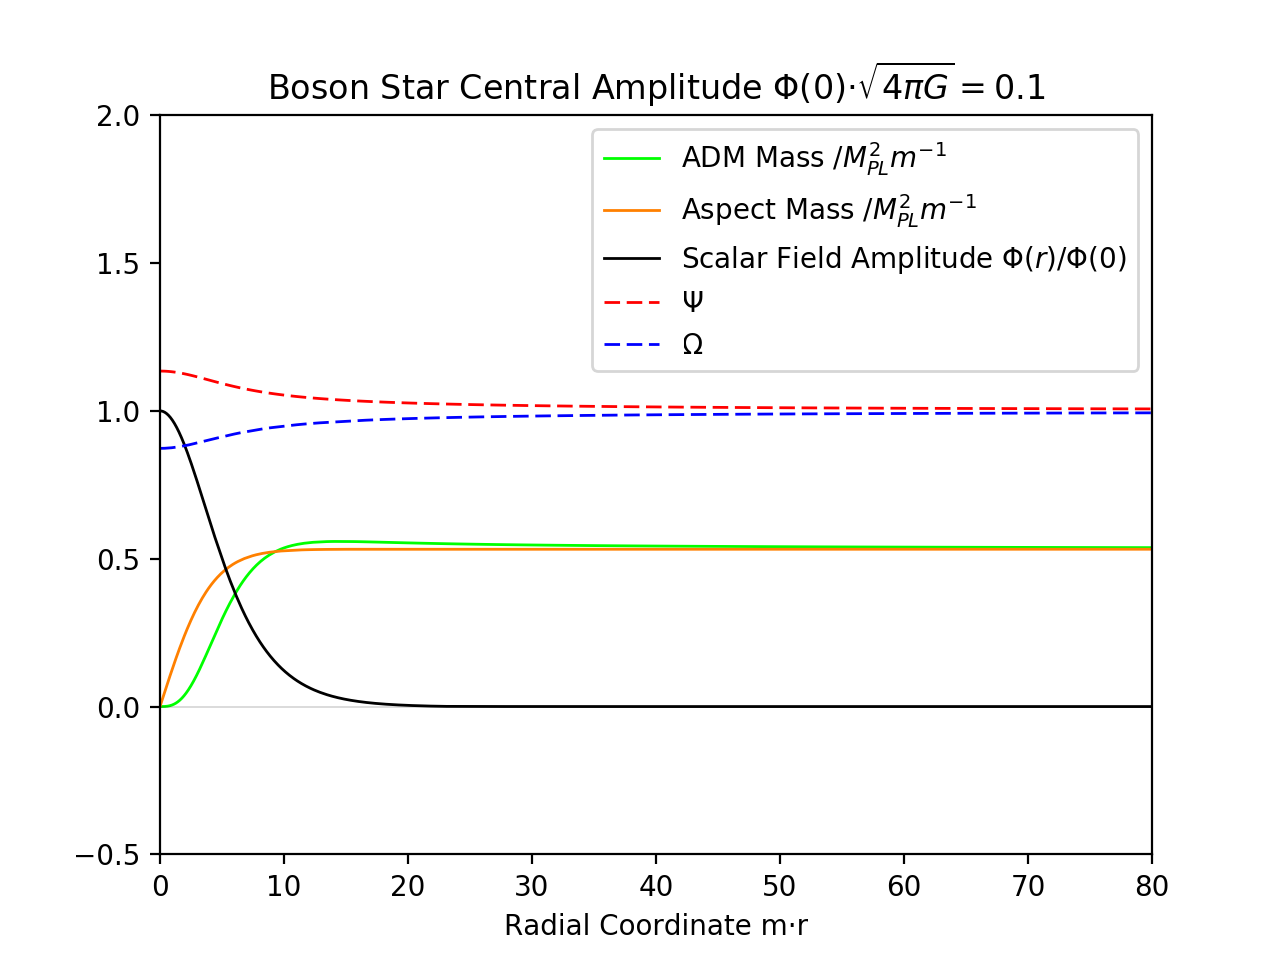
\includegraphics[width=0.5\textwidth]{png/bosonstar_groundstate.png}
%   %\hfill
%   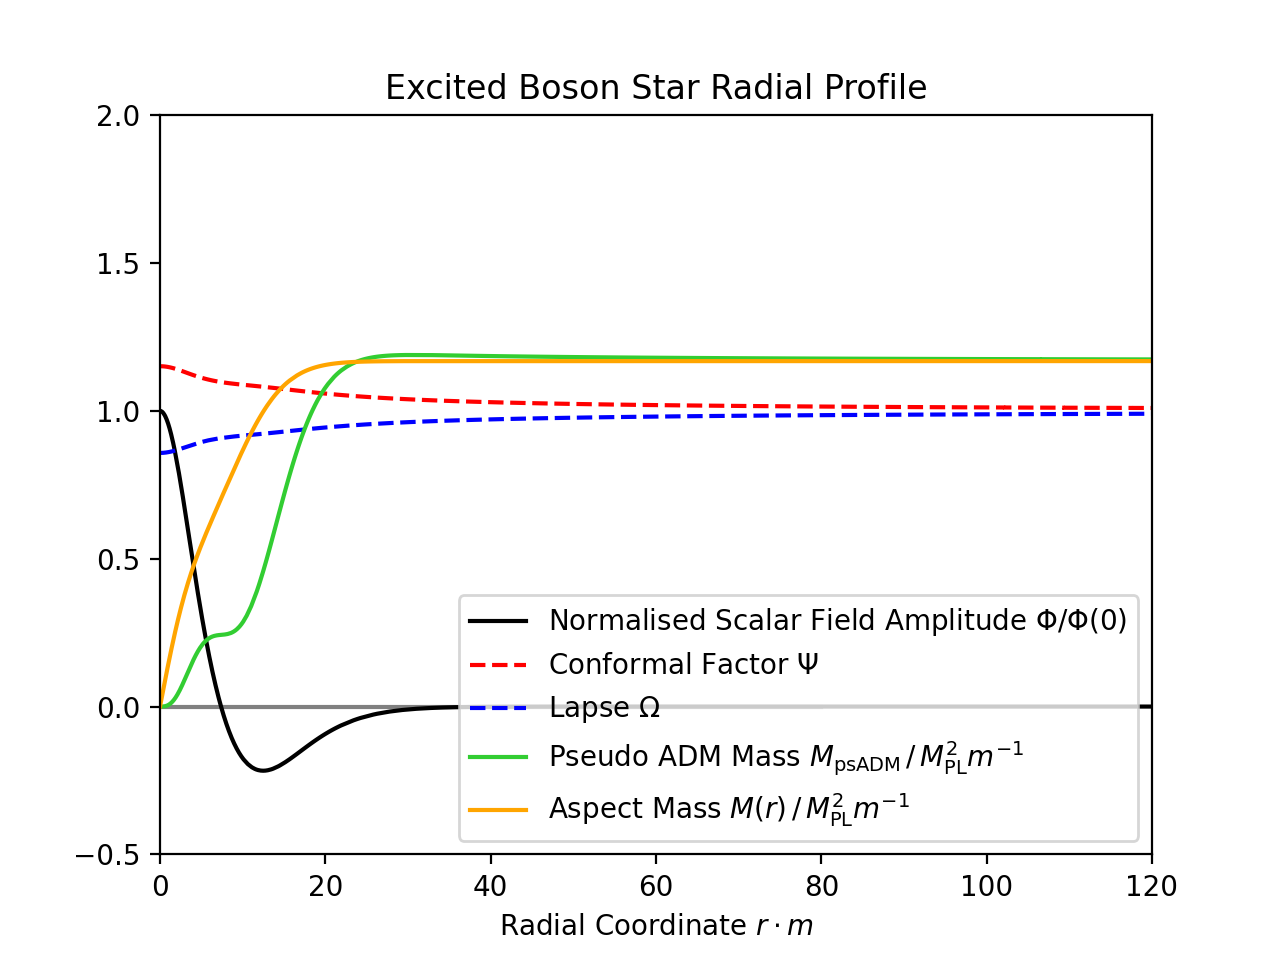
\includegraphics[width=0.5\textwidth]{png/bosonstar_excitedstate.png}
% \end{figure}

\begin{figure*}[h!]
    \subfloat%[\textsc{GRChombo}]
    {
        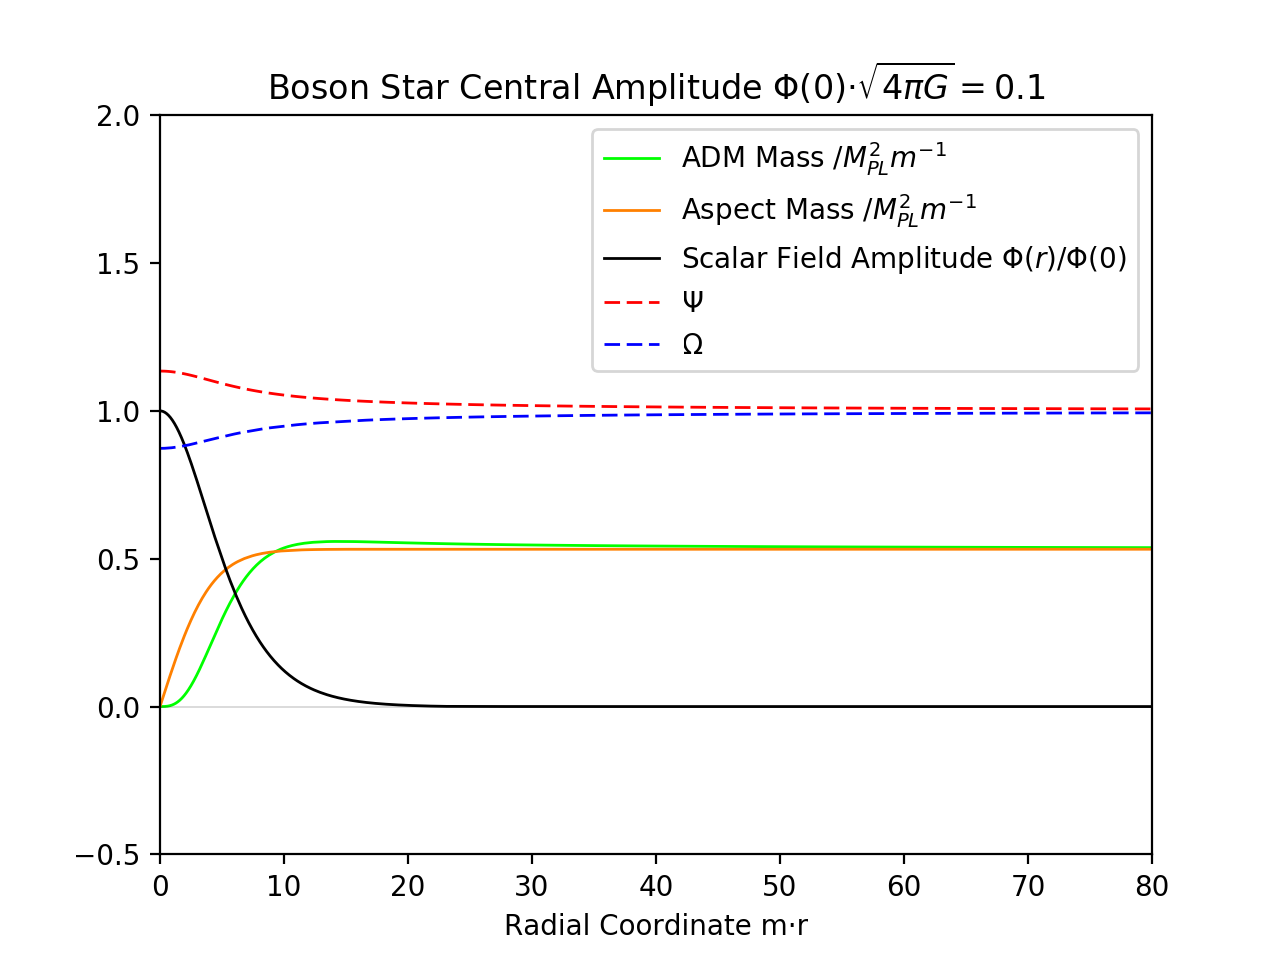
\includegraphics[width=0.48\linewidth]{png/bosonstar_groundstate.png}
        %\label{bhkick:fig:grchombo-convergence}
    }
    \hfill
    \subfloat%[\textsc{Lean}]
    {
        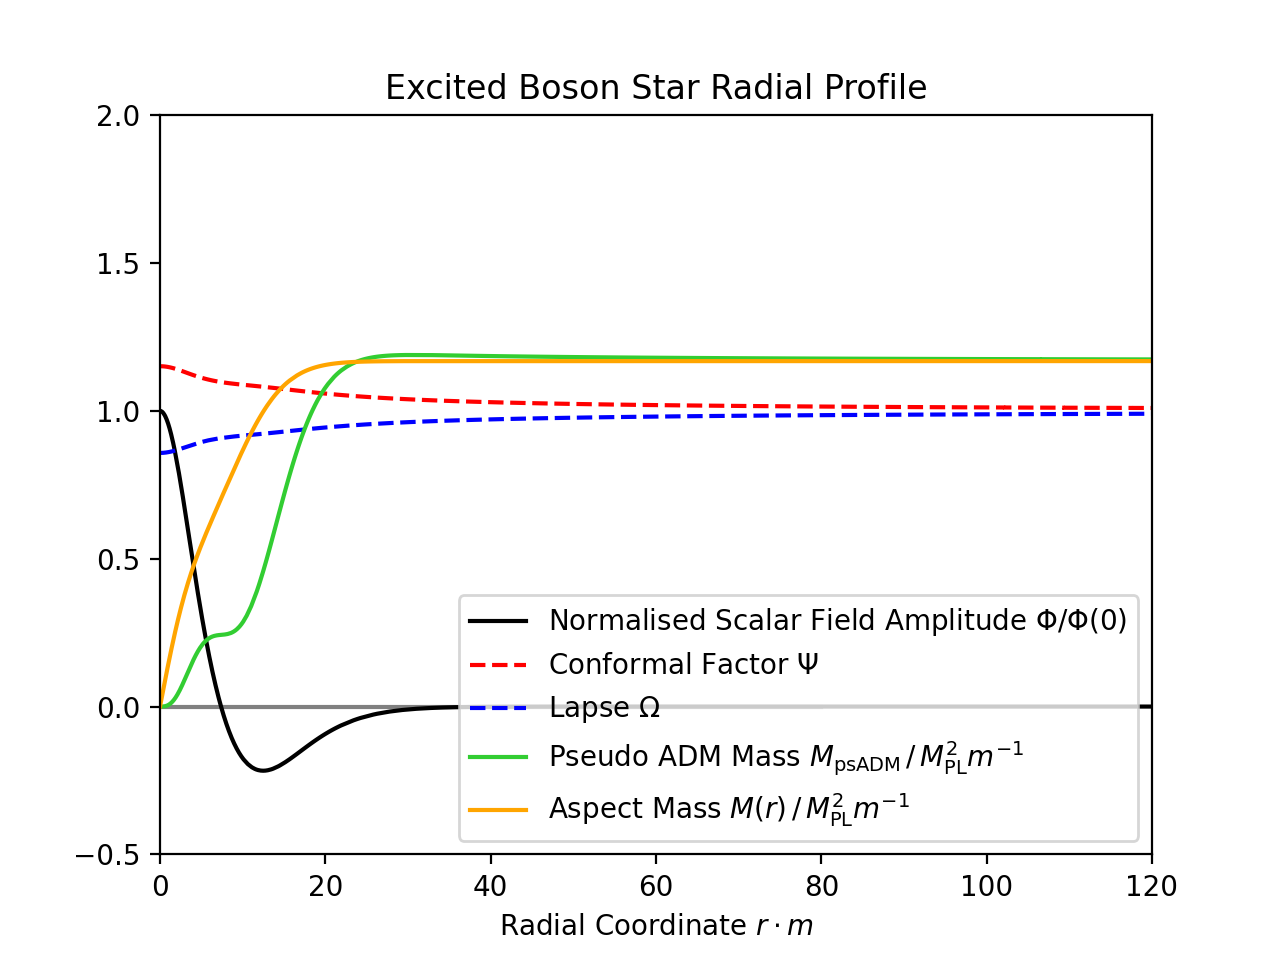
\includegraphics[width=0.48\linewidth]{png/bosonstar_excitedstate.png}
        %\label{bhkick:fig:lean-convergence}
    }
    \caption{Boson Star radial profile, Left: Ground state, Right: 1st Excited state. The ground state has an ADM mass of $M_{\rm ADM} = 0.532(5)~M_{\rm PL}^2 m^{-1}$ and the excited state has an ADM mass of $M_{\rm ADM} = 1.16(8)~M_{\rm PL}^2 m^{-1}$. Both stars have a central amplitude of $\Phi(0) \cdot \sqrt{4\pi G}=0.1 ~ m^{-1}$.
    The aspect mass is defined in Eq.~(\ref{malaise:eq:aspect_mass_def}) and the pseudo-ADM mass is given by Eq.~(\ref{boson:eq:admlike}); in the large radius limit, $M_{\rm psADM}(\infty) = M_{\rm ADM}$.}
    \label{boson:fig:f1}
\end{figure*}

%   \begin{figure}[h!]
%   \caption{Boson star radial profile for the ground state}
%   \centering
%   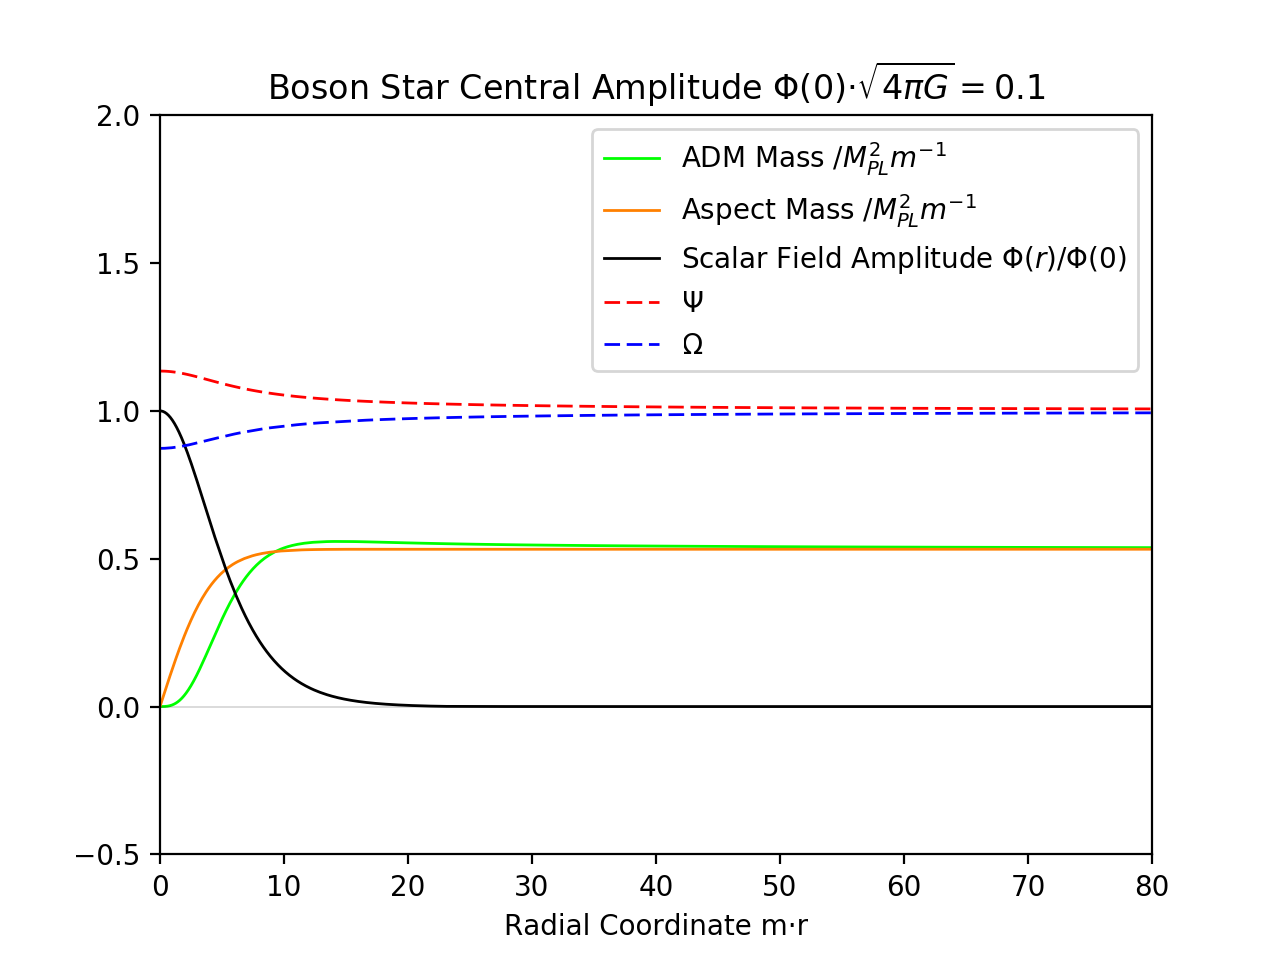
\includegraphics[width=0.8\textwidth]{png/bosonstar_groundstate.png}\label{boson:fig:f1}
% \end{figure}

%   \begin{figure}[h!]
%   \caption{Boson Star radial profile : 1st Excited state}
%   \centering
%   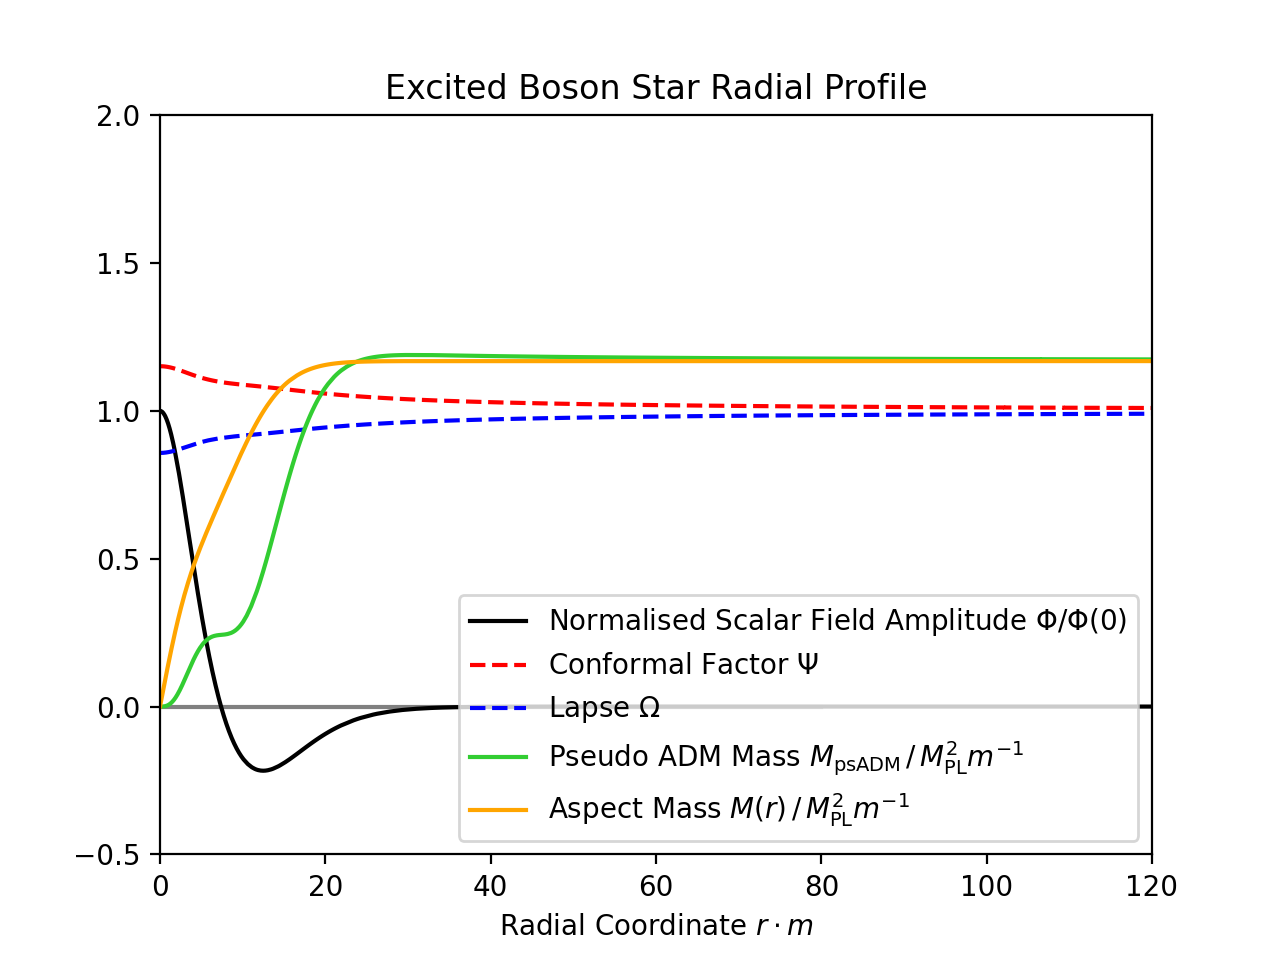
\includegraphics[width=0.8\textwidth]{png/bosonstar_excitedstate.png}\label{boson:fig:f2}
% \end{figure}


Putting everything together, a boson star solution with eigenvalue $\omega_0$
(or $\omega_n$ for excited stars) and asymptotic metric Eq.~(\ref{grchombo:eq:ABBB})
can be obtained. To find a star with asymptotic metric $\eta_{\mu\nu}$ of flat space,
the initial conditions are iteratively improved according to $\Omega_0 \rightarrow \Omega_0 /
\Omega_\infty$ and $\Psi_0 \rightarrow \Psi_0 / \Psi_\infty$; the interval bisection for
$\omega$ is then restarted. This is iterated three to five times which leaves $A=\Omega_\infty=1$
and $B=\Psi_\infty=1$ to high precision and the isotropic boson star profile has been created.
This whole process requires a few seconds runtime for a high resolution 500,000 gridpoint calculation on a regular laptop.


  \begin{figure}[h!]
  \caption{Boson star trends, Left: ADM mass vs $\Phi_0$, Right: ADM mass vs $r_{99}$}
  \centering
  \subfloat{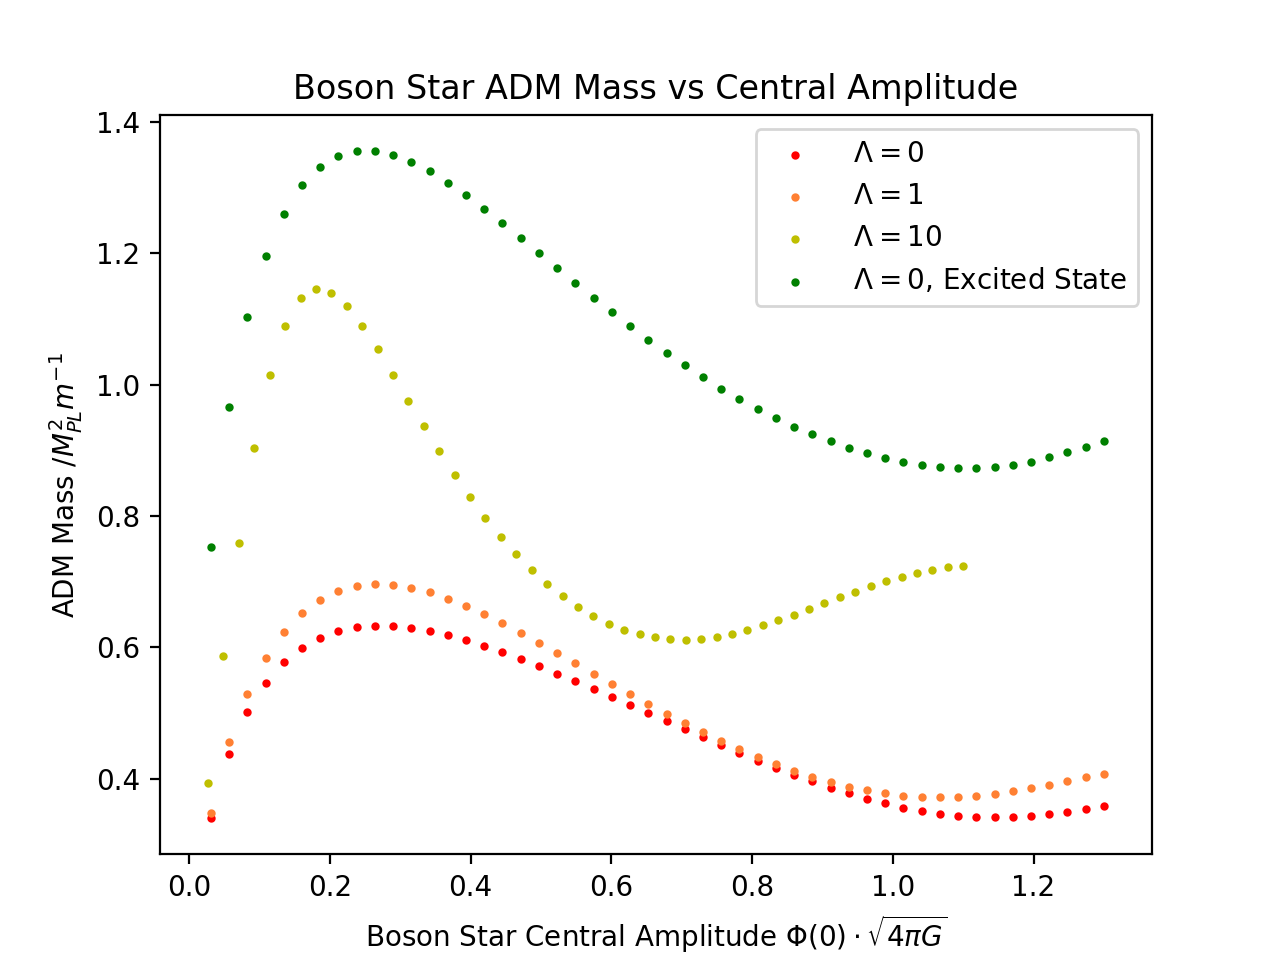
\includegraphics[width=0.48\textwidth]{png/ADM_vs_PC.png}}
  \hfill
  \subfloat{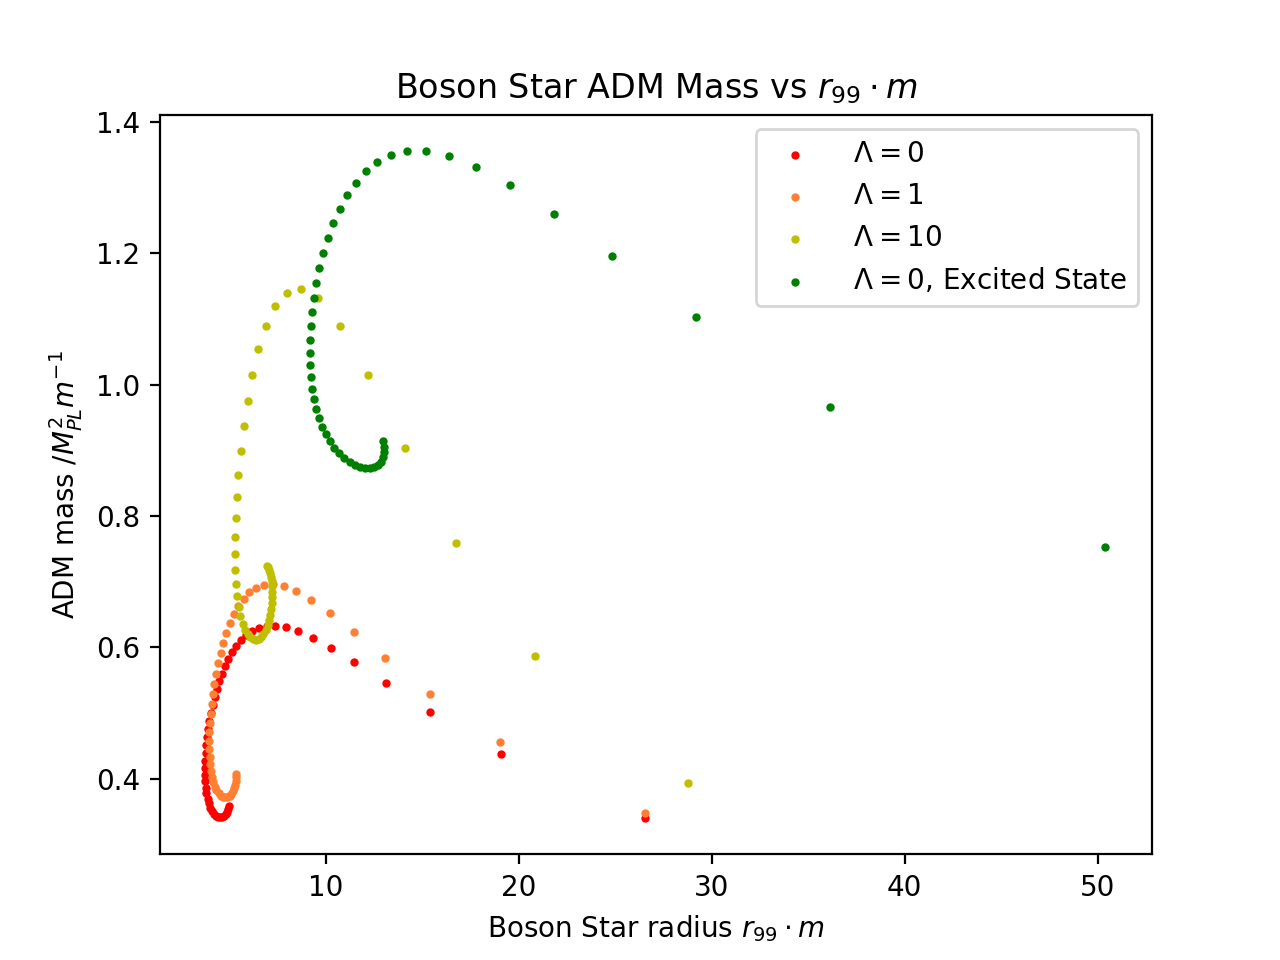
\includegraphics[width=0.48\textwidth]{png/ADM_vs_r99.png}}
  \label{boson:fig:f3}
\end{figure}

%   \begin{figure}[h!]
%   \caption{ADM mass vs $\Phi(0)$}
%   \centering
%   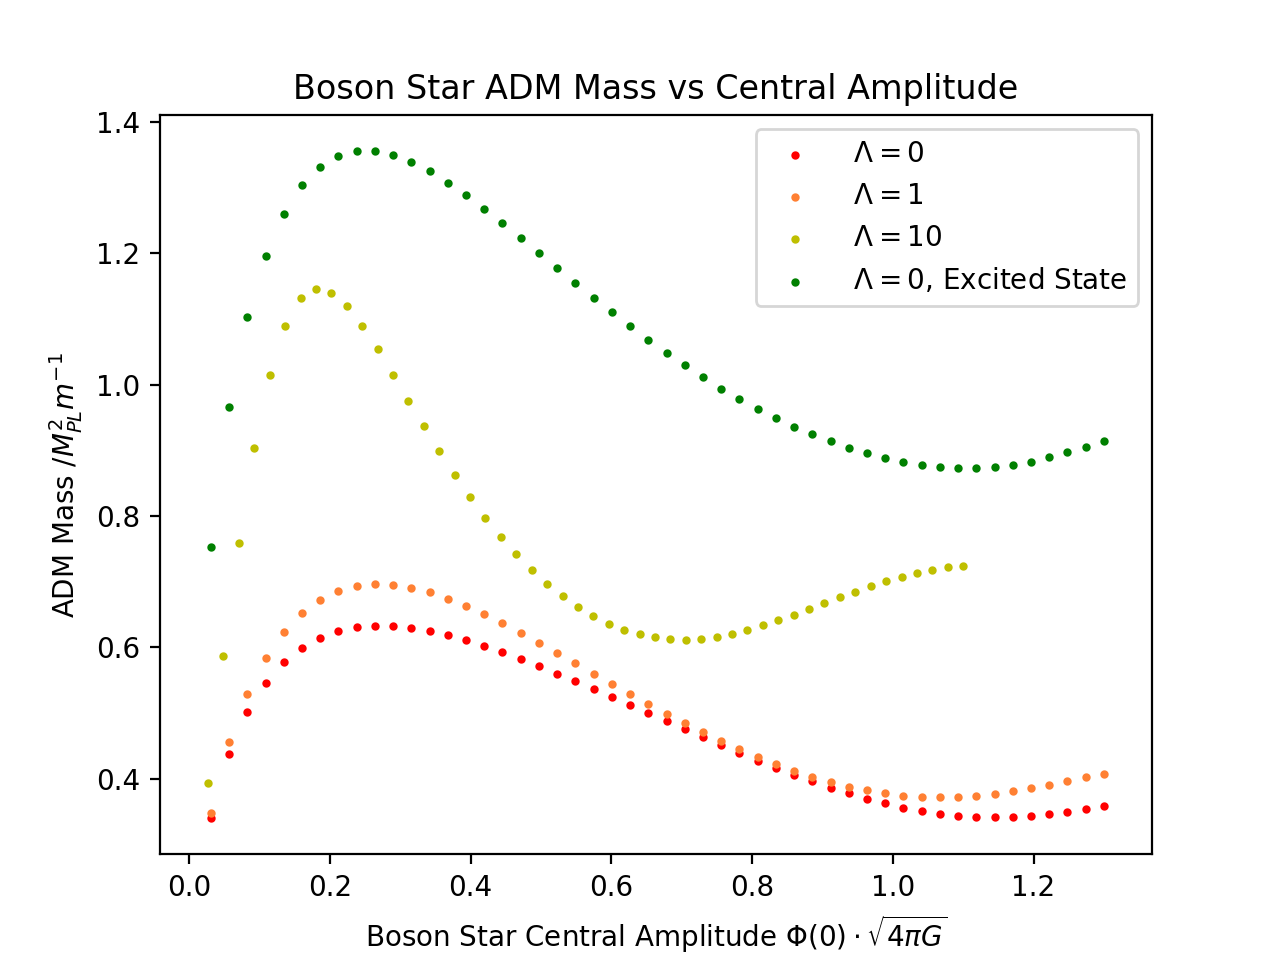
\includegraphics[width=0.8\textwidth]{png/ADM_vs_PC.png}\label{boson:fig:f1}
% \end{figure}

%   \begin{figure}[h!]
%   \caption{ADM mass vs $r_{99}$}
%   \centering
%   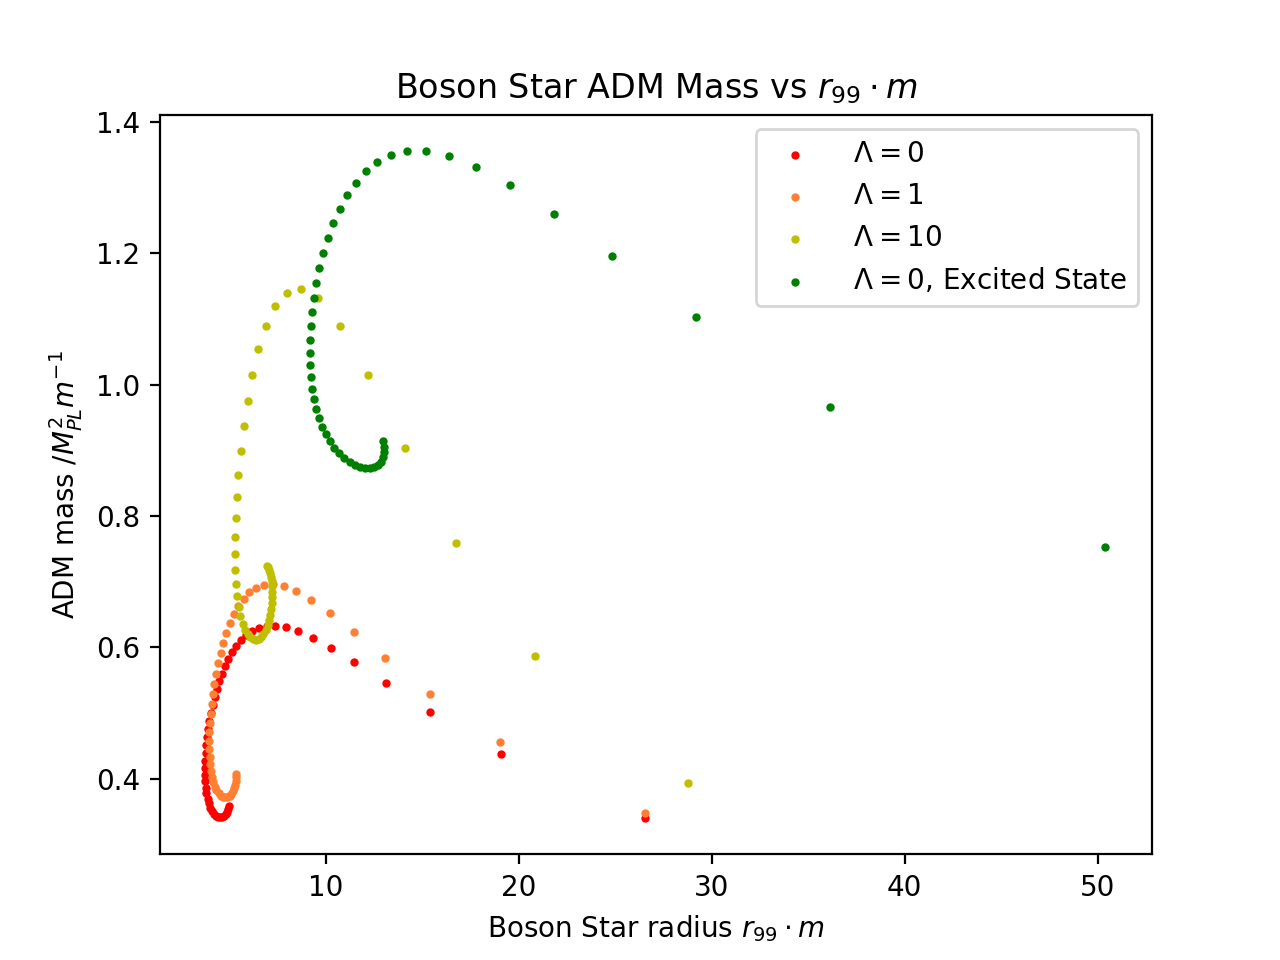
\includegraphics[width=0.8\textwidth]{png/ADM_vs_r99.png}\label{boson:fig:f2}
% \end{figure}



Figure~\ref{boson:fig:f1} shows the numerically obtained radial profile of a mini boson star ($\Lambda=0$) and an excited mini boson star. Note two mass definitions are plotted; the aspect mass defined in Eq.~(\ref{malaise:eq:aspect_mass_def}) and a pseudo-ADM mass. The conventional ADM mass \cite{arnowitt1962dynamics} is defined as
\begin{equation}
M_{\rm ADM} := \frac{1}{16\pi}\lim_{r\rightarrow\infty}\oint_{s_r} N^i \gamma^{jk}\left(\partial_j \gamma_{ik} - \partial_i \gamma_{jk} \right) \dd A,
\end{equation}
for radial coordinate $r$, 2-sphere $s_r$ of radius $r$ and unit normal vector $\bs{N}$. For an isotropic, diagonal, spherically-symmetric spatial metric ${\gamma}_{ij}$ with $\gamma_{rr} = \Psi^2(r) $, $\gamma_{\theta\theta}=\Psi^2(r)r^2$ and $\gamma_{\phi\phi}=\Psi^2(r)r^2 \sin^2\theta$ (in polar coordinates) this simplifies to,
\begin{align}
M_{\rm ADM} &= \frac{1}{16\pi}\lim_{r\rightarrow\infty}\oint_{s_r} \left(N^r \gamma^{rr}\partial_r \gamma_{rr} - N^r \gamma^{jk}\partial_r \gamma_{jk} \right) \dd A,\\
&= \frac{1}{16\pi}\lim_{r\rightarrow\infty}\oint_{s_r} N^r \Psi^{-2}\left( \partial_r \Psi^2 -  \delta^{jk}\delta_{jk}\partial_r \Psi^2 \right) \sqrt{\gamma_{\theta\theta} \gamma_{\phi\phi}} \dd \theta \dd \phi,\\
&= \frac{1}{16\pi}\lim_{r\rightarrow\infty}\int_{\theta=0}^{\theta=\pi}\int_{\phi=0}^{\phi=2\pi} -4 \Psi^{-2}\left(\partial_r \Psi \right) \Psi^2 r^2 \sin^2\theta \dd \theta \dd \phi,\\
&= \lim_{r\rightarrow\infty} \left(- r^2 \partial_r \Psi\right) ,\\
\end{align}
where we used the fact that $\bs{\gamma}(\bs{N},\bs{N})=1$ which gives $N^r = (\gamma_{rr})^{-1/2} = \Psi^{-1}$.
Note that for a Schwarzschild black hole with $\Psi = \left(1+\frac{M}{2r} \right)^2$ the ADM mass formula returns
the expected result of $M$. We define the {\it pseudo-AMD mass} as
\begin{equation}
M_{\rm psADM}(r):=- r^2 \partial_r \Psi ,\label{boson:eq:admlike}
\end{equation}
which of course satisfies $M_{\rm ADM} = M_{\rm psADM}(\infty)$.

 Polytropic fluid star initial data has also been calculated as a preliminary test
 of the code; they are easier to create as they do not require solving an eigenvalue
 problem and do not have an asymptotically growing mode. Figure~(\ref{boson:fig:f3})
 shows how the ADM mass of boson stars varies with central amplitude $\Phi_0$ and
 $r_{99}$, the radius which $\Phi(r_{99}) = \Phi_0/100$. It should be noted that
 the mini boson star (with $\Lambda =0$) case agrees with the known maximum mass,
 the Kaup limit \cite{PhysRev.172.1331} $M_{\rm max} \approx 0.633 {M_{\rm PL}^2}{m^{-1}}$
 with the largest mass being $ M_{\rm max} = 0.63299(3) {M_{\rm PL}^2}{m^{-1}} $
 corresponding to a central amplitude of $ \sqrt{4\pi G}(\Phi_0)_{\rm max} = 0.271(0)~m^{-1}$.



While many different boson stars have been computed to test the initial data code,
all the following evolutions use the same boson star with parameters $\Lambda=0$,
$\sqrt{4\pi G}\Phi_0=0.1~m^{-1} \rightarrow \Phi_0 \approx 0.0282~m^{-1}$ and
ADM mass $M=0.532(7)~M_{\rm PL}^2 m^{-1}$. This is as the stars are heavy enough
to form black holes under collisions and large deformations, but stable enough
to not collapse to a black hole for moderate perturbations.




\subsection{Single Star Evolution}

As a check that the initial data from section \ref{grchombo:sec:initialdata} is correct,
a mini boson star with central density $\Phi_0=0.02820~m^{-1}$ is evolved in time
in three spatial dimensions. The simulation has a physical domain size $L=1024~m^{-1}$
with $N=320$ gridpoints on AMR level zero with grid spacing $\Delta x = 3.2~m^{-1}$.
The AMR is allowed up to six extra levels; the finest level (level six) has a grid
spacing of $\Delta x = 0.05~m^{-1}$. The star is supposed to remain in the centre
of the grid and not change as it is a rest frame soliton; this is observed through
evolution with {\sc GRChombo}. Figure (\ref{boson:fig:f5}) shows the global maximum
value of $|\vp|$ (left figure) and the total integral of the Noether charge ${N}$
over the grid (right figure). As can be seen, $|\vp|_{\rm max}$ is constant to
$\sim 0.7\%$ and $N$ is conserved to the $\sim 0.07\%$ level until time $t=320~m^{-1}$.

  \begin{figure}[h!]
  \caption{Left: Maximum of $|\vp|$ during the evolution, Right: Total integrated Noether charge $N$.
  The initial noise seen in the two figures is attributed to junk radiation from
  refinement boundaries and is potentially exacerbated by the gauge settling from
  the initial gauge to the moving puncture gauge used. The lower-amplitude oscillation
  seen continuously in the left figure is due to finite resolution when calculating
  the maximum value $\varphi_{\rm max} = [{\rm Re}(\varphi)^2 + {\Im}(\varphi)^2]_{\rm max}$
  on any gridpoint. }
  \centering
  \subfloat{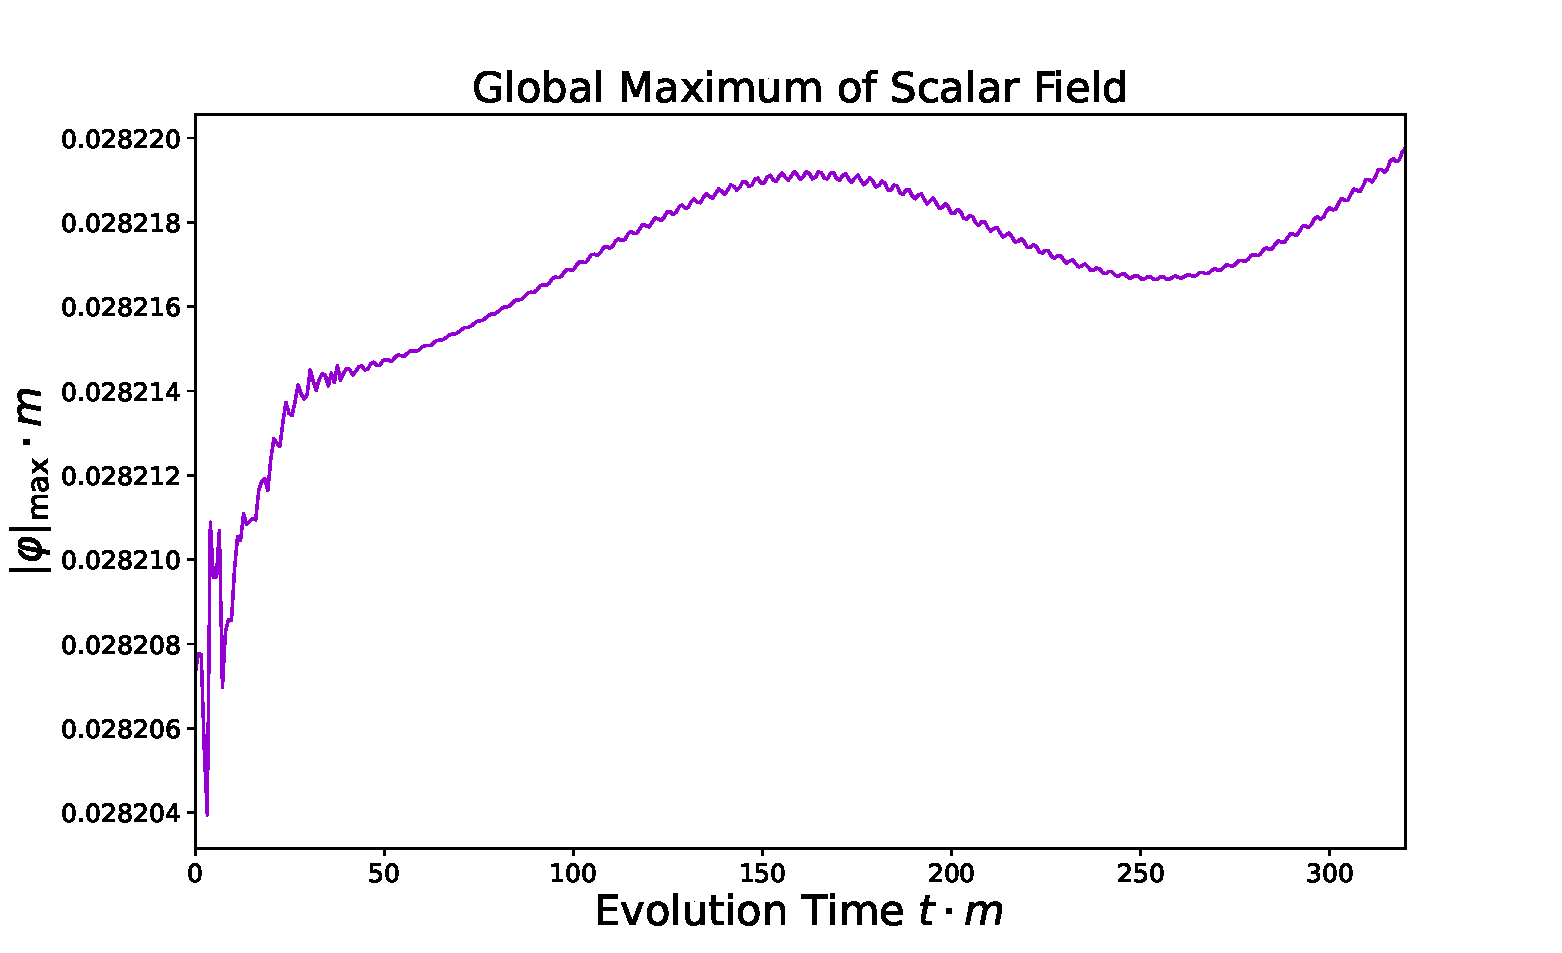
\includegraphics[width=0.5\textwidth]{data/star_modphi_nicer.pdf}}
  \hfill
  \subfloat{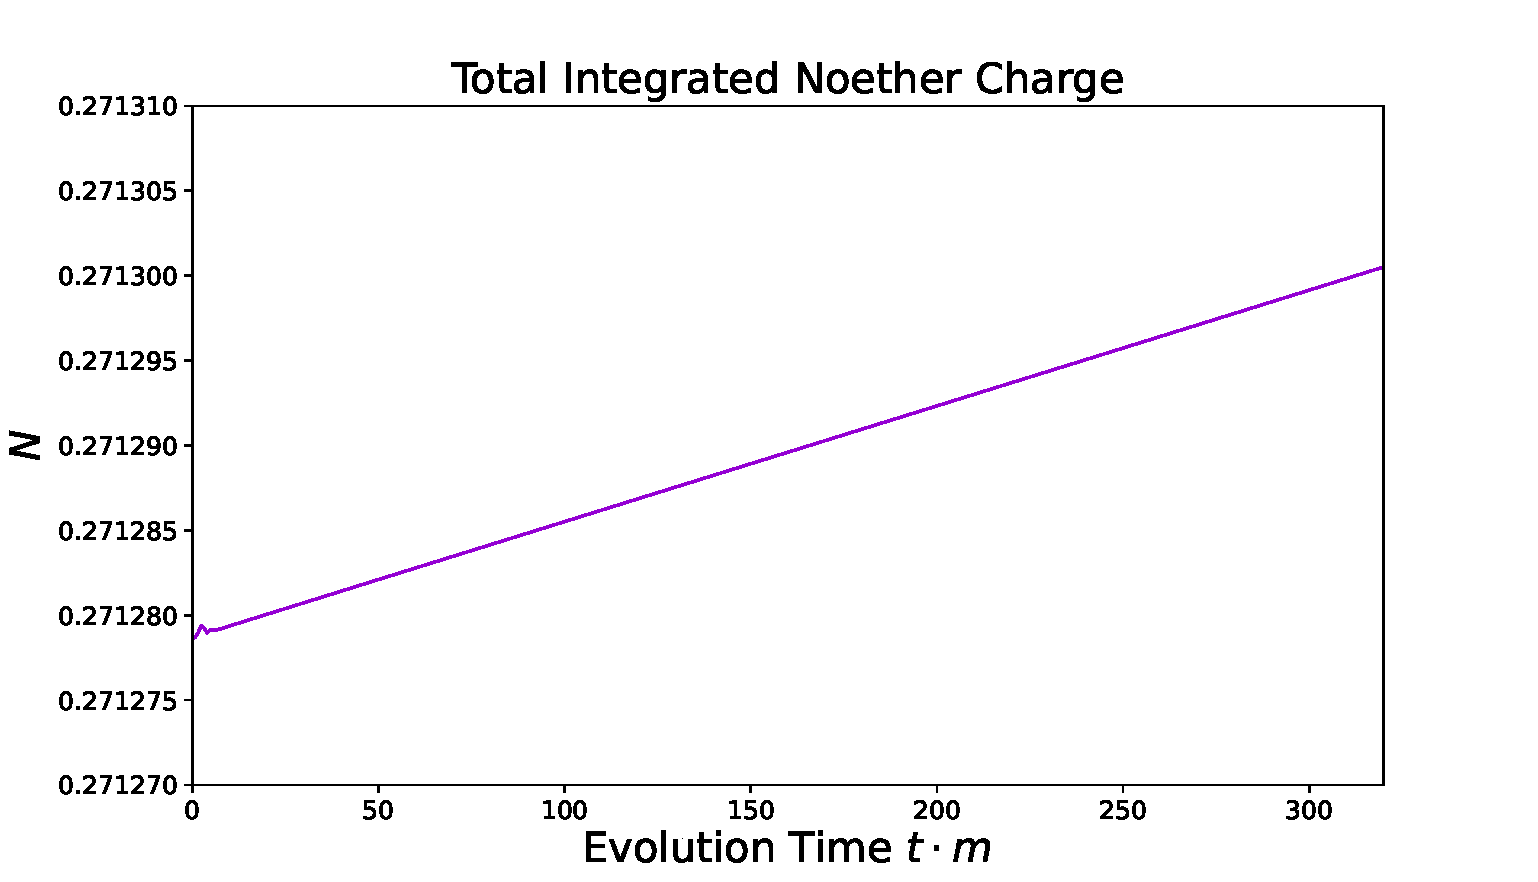
\includegraphics[width=0.5\textwidth]{data/star_N_nicer.pdf}}
  \label{boson:fig:f5}
\end{figure}






\subsection{Superposition of Initial Data} \label{grchombo:sec:superposition}
In order to simulate a spacetime consisting of two stars (or a star and a black hole) we must choose a way of superposing the initial data of two objects, centred at $x^{(1)}$ and $x^{(2)}$. For some field $\psi^{(j)}$ associated with the compact object at $x^{(j)}$,
\begin{equation}
\psi^{(j)} = \psi(x-x^{(j)}),
\end{equation} where $\psi$ refers to the object centred about the origin.
Taking two compact objects with fields $\vp$, $\Pi$, $\gamma_{ij}$, $\K_{ij}$, $\alpha$ and $\beta^i$, a naive superposition scheme was chosen;
\begin{align}
 \vp &= \vp^{(1)} + \vp^{(2)},\\
\Pi &= \Pi^{(1)} + \Pi^{(2)},\\
 \K^i_j &= {\K^{(1)}}^i_j+{\K^{(2)}}^i_j,\\
 \gamma_{\mu\nu} &= \gamma^{(1)}_{\mu\nu} + \gamma^{(2)}_{\mu\nu}-\delta_{\mu\nu},\\
\beta_i &= \beta^{(1)}_i + \beta^{(2)}_i ,\\
 \alpha &= \sqrt{\alpha_{(1)}^2 + \alpha_{(2)}^2-1},\\
 \chi &= \det\left(\gamma^{(1)}_{\mu\nu} + \gamma^{(2)}_{\mu\nu}-\delta_{\mu\nu}\right)^{-1/3},
 \end{align}
where the super-scripts ${}^{(1)}$ and ${}^{(2)}$ refer to the separate compact objects. The extrinsic curvature is chosen to be superposed with mixed indices so that it implies the trace $\mathcal{K}$ is also superposed. If one of the compact objects is a black hole the lapse $\alpha \rightarrow 0$ on the horizon; this is circumvented by setting,
\begin{equation} \alpha = \sqrt{\chi},\end{equation}
ensuring that the lapse is real and non-negative everywhere on $\Sigma_t$.

Superposing two solutions in general relativity usually no longer satisfies the Einstein equation; the Hamiltonian constraint Eq.~(\ref{nr:eq:ham}) and momentum constraints Eq.~(\ref{nr:eq:mom}) are violated. For asymptotically flat compact objects, the constraint violation reduces to zero as the object separation tends to infinity. In the case of finite separations, the CCZ4 scheme in section \ref{nr:sec:ccz4} aims to drive the constraint violation towards zero and hence a true solution of Einstein's equation; in practice, the CCZ4 scheme is more efficient at damping low amplitude, high-frequency violations and will not fully reduce long-wavelength violations \cite{gundlach2005constraint}. The collisions of compact objects in section \ref{grchombo:sec:bscollisions} use this naive superposition scheme. Section \ref{mal:sec:improvedsuperposition} explores a technique to improve the naive superposition of compact objects.



















\subsection{Collisions of Boson Stars}\label{grchombo:sec:bscollisions}



Both a headon collision and a grazing collision of two boson stars are simulated
using the superposition scheme given in section \ref{grchombo:sec:superposition}.
The two stars are identical, each has a central density of $\Phi_0=0.02820~m^{-1}$
and an ADM mass $M=0.532(7) ~M_{\rm PL}^2m^{-1}$. The stars are placed at positions
$x^i=\pm\{40,0,0\}~m^{-1}$ in the headon case and $x^i=\pm\{40,8,0\}~m^{-1}$ in
the grazing case and are boosted together with respective velocities $v^i=\mp\{0.1,0,0\}$
in both cases. A speed of $v=0.1$ corresponds to a rapidity of $\psi=0.1003353$.
The simulations have a physical domain size of $L=512~m^{-1}$ with $N=256$ gridpoints
on AMR level zero, this gives a coarse grid resolution of $\Delta x = 2~m^{-1}$.
There are up to five extra AMR levels giving a finest grid resolution of $\Delta x = 1/16~m^{-1}$.




\subsubsection{Headon Collision}
 \begin{figure}[h!]
  \caption{Left: Maximum of $|\vp|$ during evolution, Right: Total integrated Noether charge $N$.}
  \centering
  \subfloat{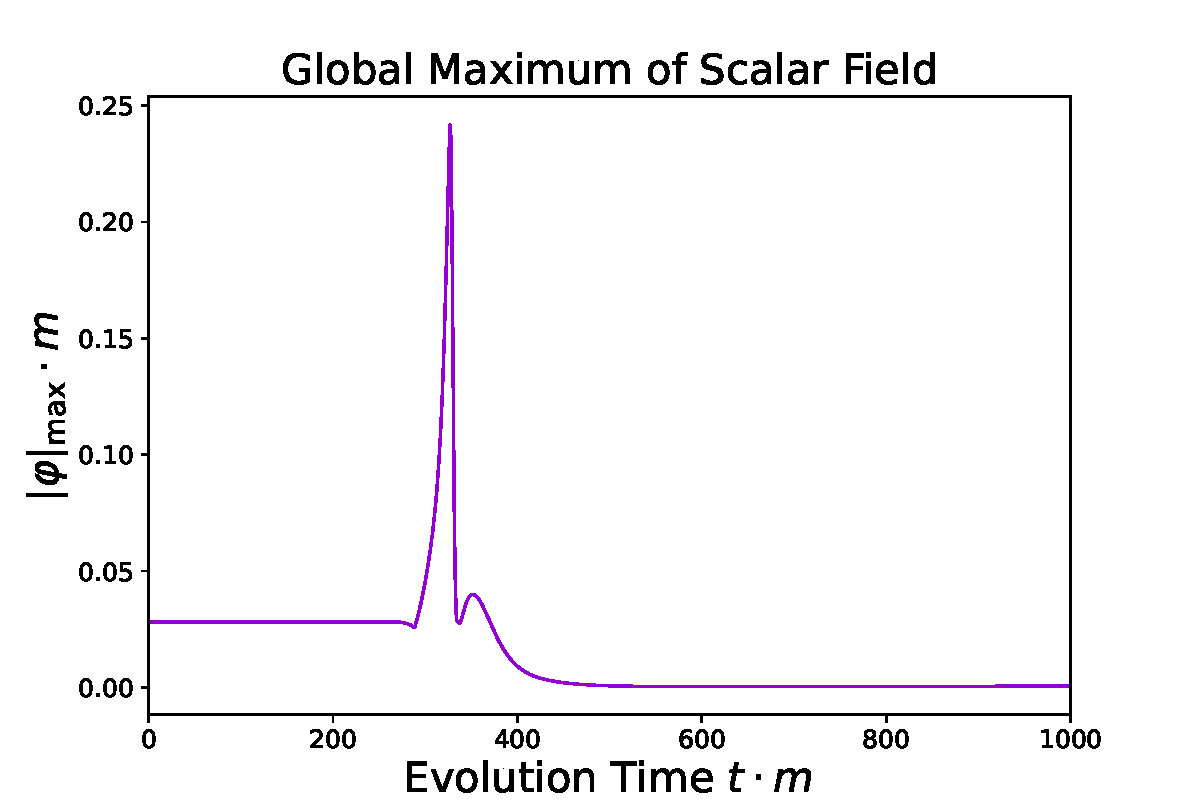
\includegraphics[width=0.5\textwidth]{data/headon_modphi_nicer.pdf}}
  \hfill
  \subfloat{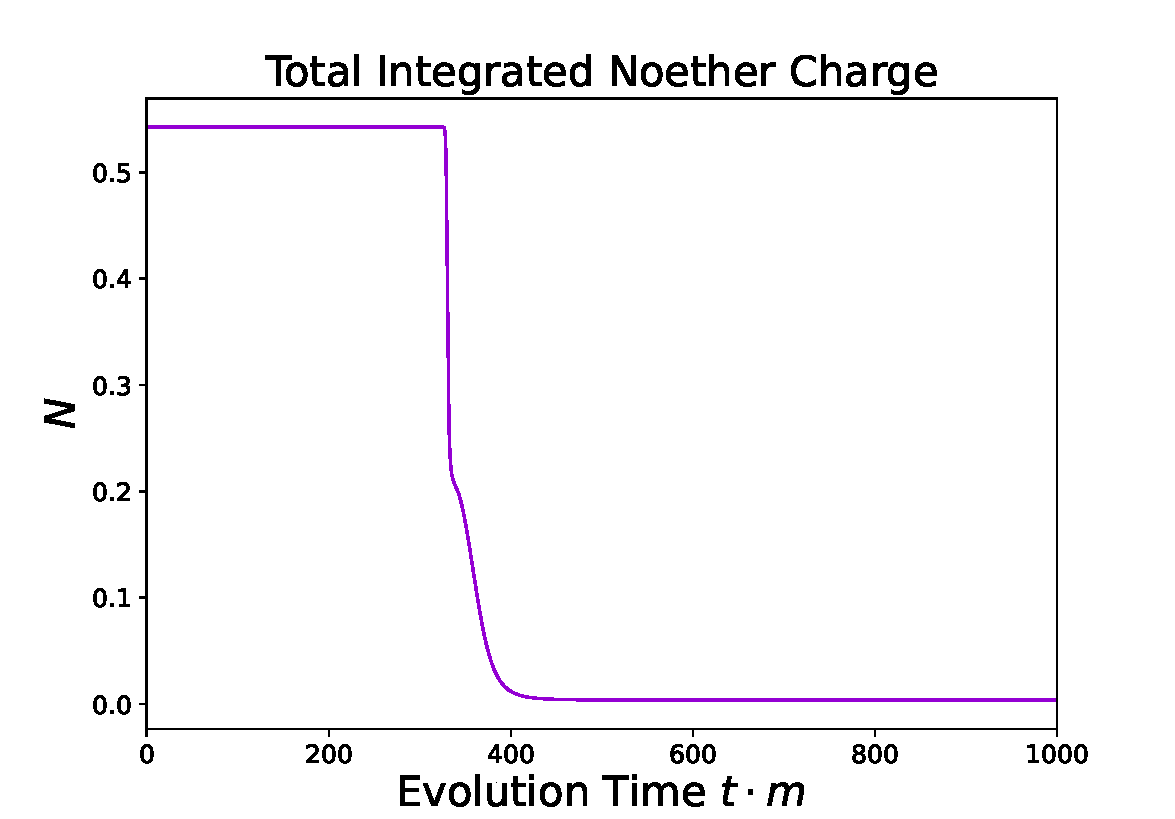
\includegraphics[width=0.5\textwidth]{data/headon_N_nicer.pdf}}
  \label{boson:fig:f7}
\end{figure}

\begin{figure}[h!]
  \caption{Gravitational wave signal of the headon boson star collision. The $l,m=2,2$ and $l,m=2,0$ spin weighted spherical harmonic modes of the $\Psi_4$ Newman-Penrose scalar are given.}
  \centering
  \subfloat{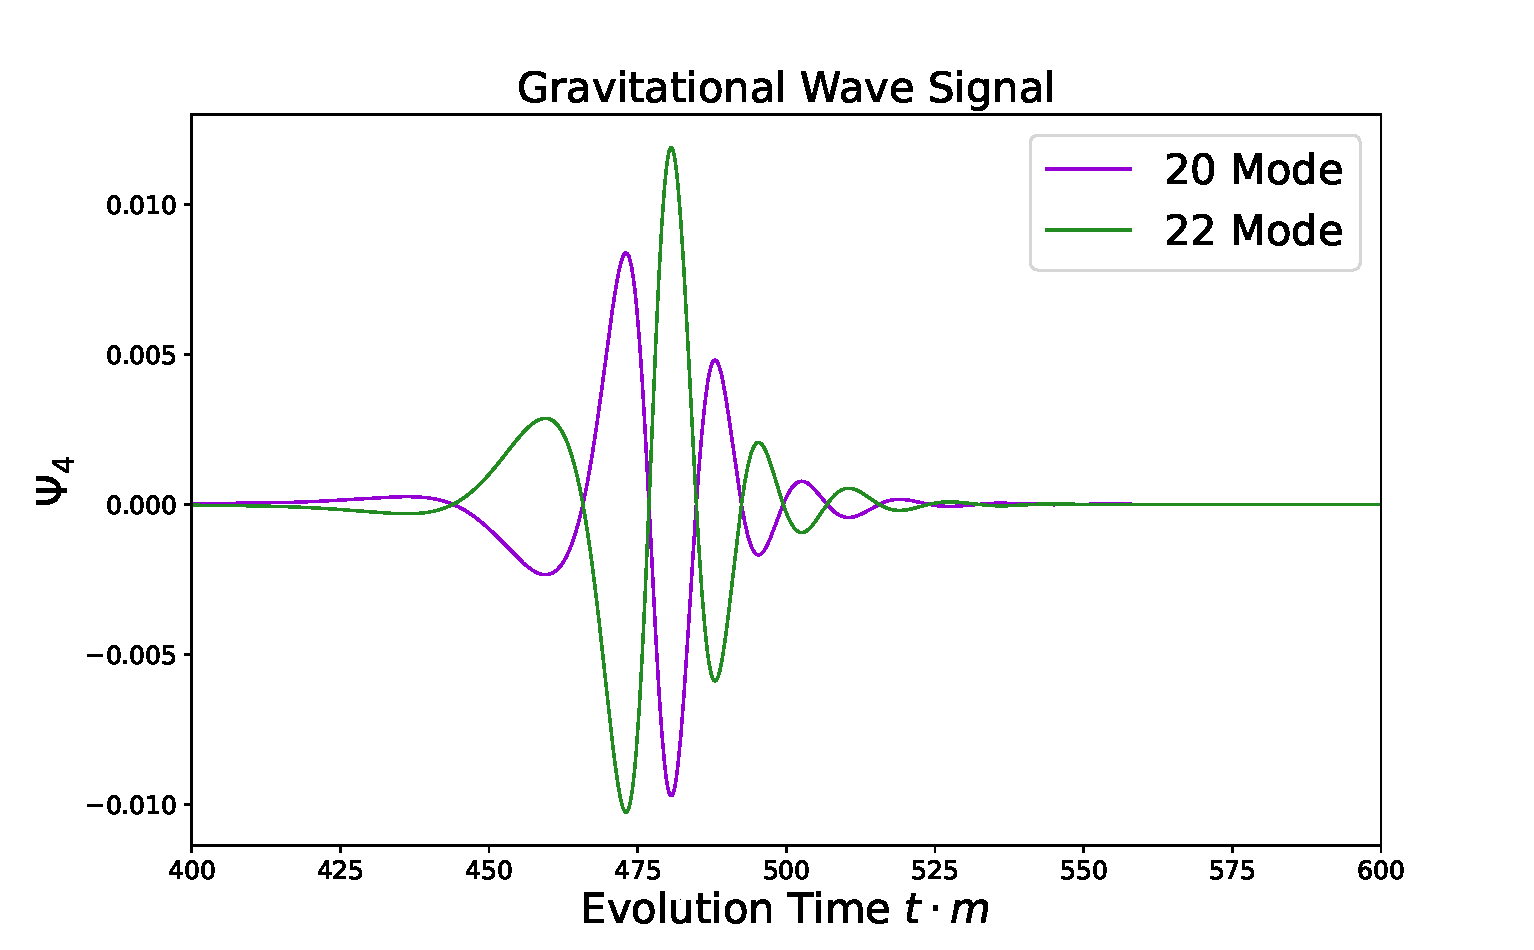
\includegraphics[width=0.5\textwidth]{data/headon_weyl_nicer.pdf}}\label{boson:fig:f9}
\end{figure}

Figure (\ref{boson:fig:f7}) shows $|\vp|_{\rm max}$, the global maximum value of $|\vp|$, and the total Noether charge $N$ as a function of time for the headon collision. At time $t\approx 289 ~m^{-1}$, $|\vp|_{\rm max}$ rapidly increases and then drops to zero, signalling the collapse to a black hole. At time $t\approx 327~m^{-1}$, there is a temporal maximum in $|\vp|_{\rm max}$ as the resolution limit of the simulation is reached and the scalar field is dissipated by the Kreiss-Oliger dissipation and diverging resolution requirements. This dissipation can also be seen in the Noether charge plot at a time of $t \approx 326~m^{-1}$ where the total charge that should remain constant but begins to fall. The lack of sufficient resolution inside the black hole is however not problematic for the external simulation; the errors accumulated are trapped inside the event horizon. Figure~(\ref{boson:fig:f7}) shows that the total Noether charge rapidly decays to zero at late time as it falls into the black hole and is dissipated.


The gravitational wave extraction at radius $r=140~m^{-1}$ is given in figure \ref{boson:fig:f9}. A spin-weighted spherical harmonic decomposition of the Newman-Penrose scalar $\Psi_4$ has been done and the $l,m = 2,0$ and $l,m = 2,2$ modes are plotted.


The dynamics of the two boson stars are shown in Fig.~(\ref{boson:fig:ff7}) which plots the scalar field modulus $|\vp|$ in the $x,y$ plane. The stars collide at time $275~m^{-1} < t < 300~m^{-1}$; which compares well to the Newtonian collision time\footnote{A simulation of point masses in Newtonian physics has been done to extract a collision time.} $t = 287.6~m^{-1}$ of two point masses with the same initial conditions. Soon after collision, an over-density of the scalar field develops which subsequently collapses to a black hole. The black hole then accretes the surrounding scalar field; the scalar field can be seen to be composed of higher order spherical harmonic modes at later times.






\subsubsection{Grazing Collision} \label{grchombo:sec:graze}

Figure (\ref{boson:fig:f10}) plots $|\vp|_{\rm max}$ and the total Noether charge
($N$) versus time for the grazing collision. At time $t\approx 309~m^{-1}$,
$|\vp|_{\rm max}$ rapidly increases and a black hole is soon formed. The black
hole is assumed\footnote{No horizon measure, or measure of angular
momentum of matter
falling into the black hole, has been done for this simulation -
these measures would be warranted in any future study.}
to be spinning due to the collapsing matter containing angular
momentum. At time $t\approx 356 ~m^{-1}$ there is a temporal maximum in $|\vp|_{\rm max}$;
similarly to the headon collision, this is caused by diverging resolution requirements
near the black hole centre and does not affect the exterior spacetime. Consequently,
the Noether charge plot shows a drop in charge at a time of $t \approx355~m^{-1}$.
 \begin{figure}[h!]
  \caption{Left: Maximum of $|\vp|$ during evolution, Right: Total integrated Noether charge $N$.}
  \centering
  \subfloat{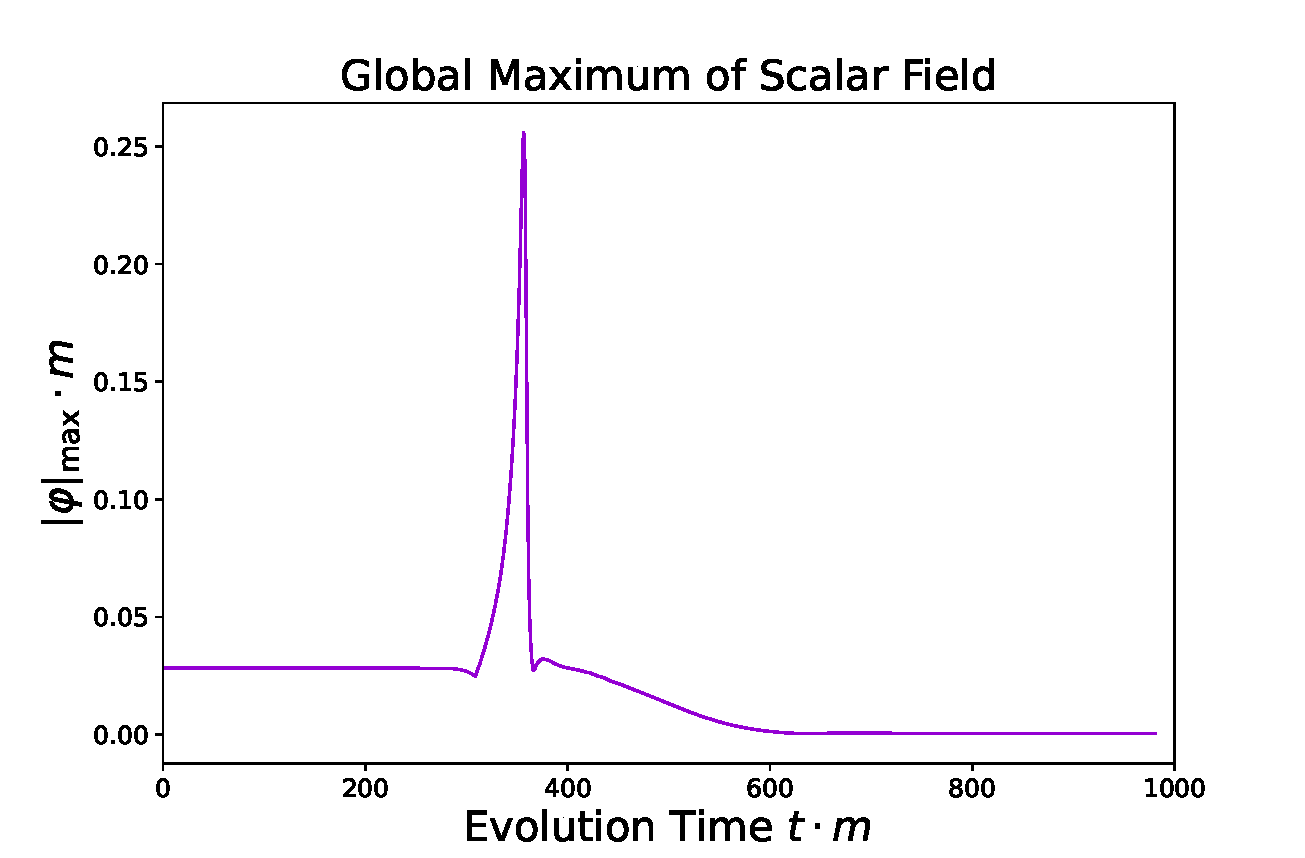
\includegraphics[width=0.5\textwidth]{data/graze_modphi_nicer.pdf}}
  \hfill
  \subfloat{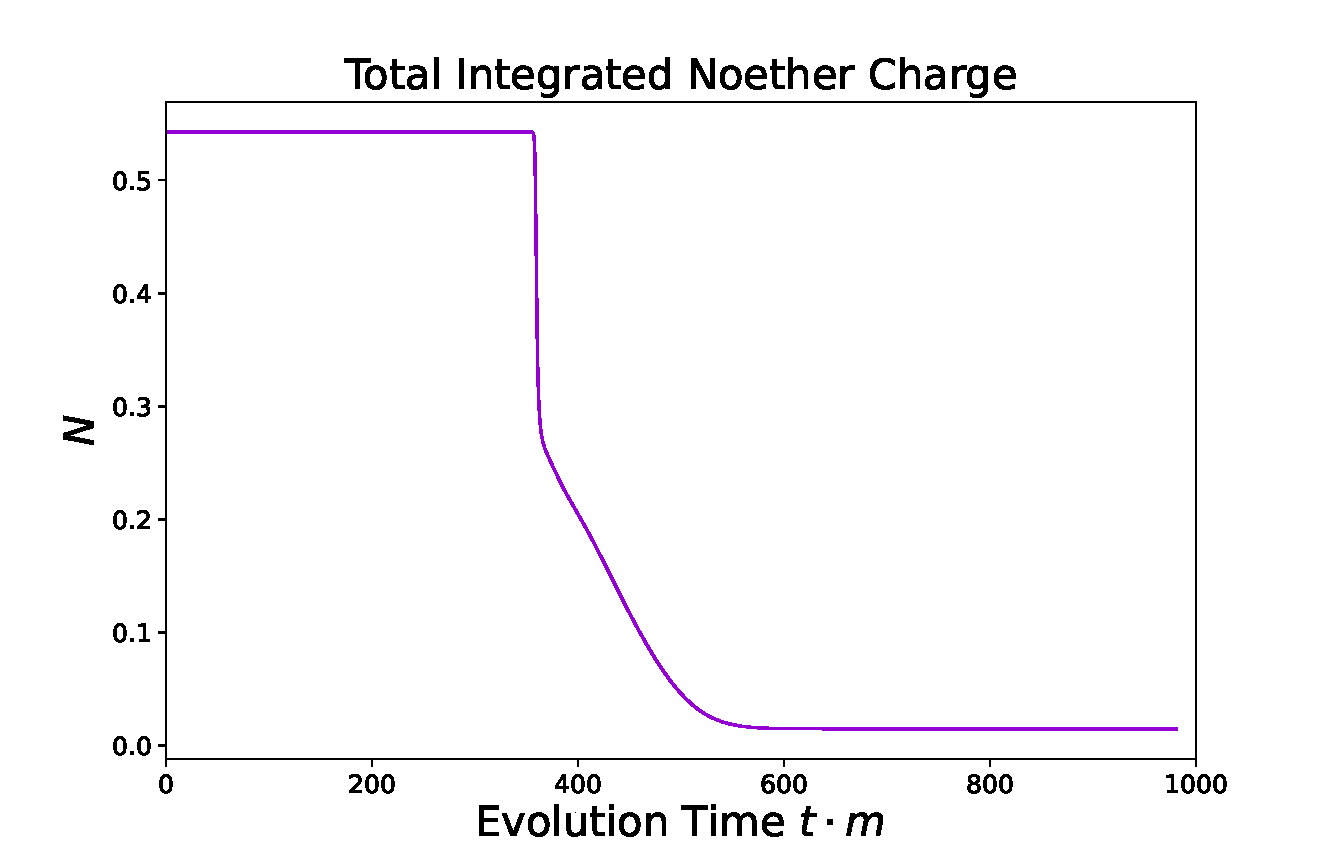
\includegraphics[width=0.5\textwidth]{data/graze_N_nicer.pdf}}
  \label{boson:fig:f10}
\end{figure}



A simulation of the grazing collision with point masses has been done using Newtons laws. The time taken for closest approach (with separation $s = 2.33~m^{-1}$) is $t=315.8~m^{-1}$; at this separation the finite sized stars would collide. Snapshots of the grazing boson star collision using numerical relativity (in full general relativity) are shown in Fig.~(\ref{boson:fig:ff10}) plotting the scalar field modulus $|\vp|$ in the $x,y$ plane. The stars collide at time $300~m^{-1} < t < ~m^{-1}$ which is in good agreement with the Newtonian approximation. Soon after collision, an over-density of the scalar field develops and collapses to a black hole; this black hole is thought to be spinning due to the angular momentum of the collapsing matter. The black hole subsequently accretes most of the surrounding scalar field leaving a quasi-long-lived rotating toroidal scalar field configuration surrounding the black hole. This late time toroidal scalar field configuration will be referred to as a {\it toroidal wig} due to it being \enquote{fake} hair. The late time toroidal wig seems to settle to a rotationally symmetric configuration, with no quadrupole moment, and does not emit a significant gravitational wave signal; this can be seen in Fig.~(\ref{boson:fig:f12}) which plots the $l,m=2,2$ and $l,m=2,0$ modes of $\Psi_4$.



\begin{figure}[h!]
  \caption{Gravitational wave signal of the grazing boson star collision. The $l,m=2,2$ and $l,m=2,0$ modes of the $\Psi_4$ Newman-Penrose scalar are given.}
  \centering
  \subfloat{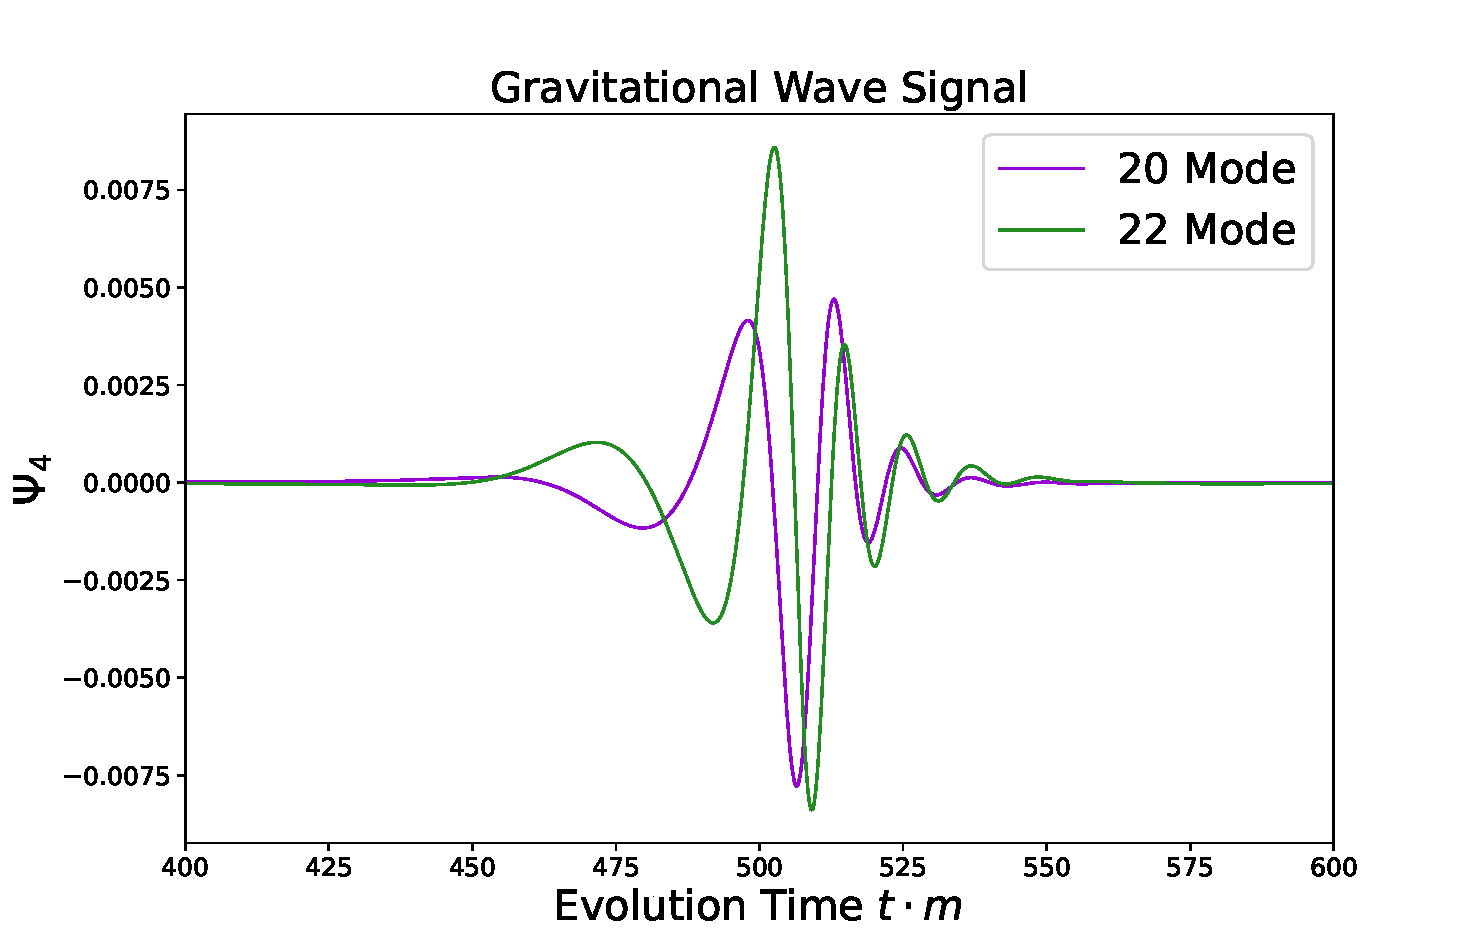
\includegraphics[width=0.5\textwidth]{data/graze_weyl_nicer.pdf}}
  \label{boson:fig:f12}
\end{figure}

 \begin{figure}[h!]
\caption{Left: Comparison of late time Noether charge $N$ between headon collision and grazing collision of two boson stars. Right: Late time plot of the Noether charge of the grazing collision only.}
\subfloat{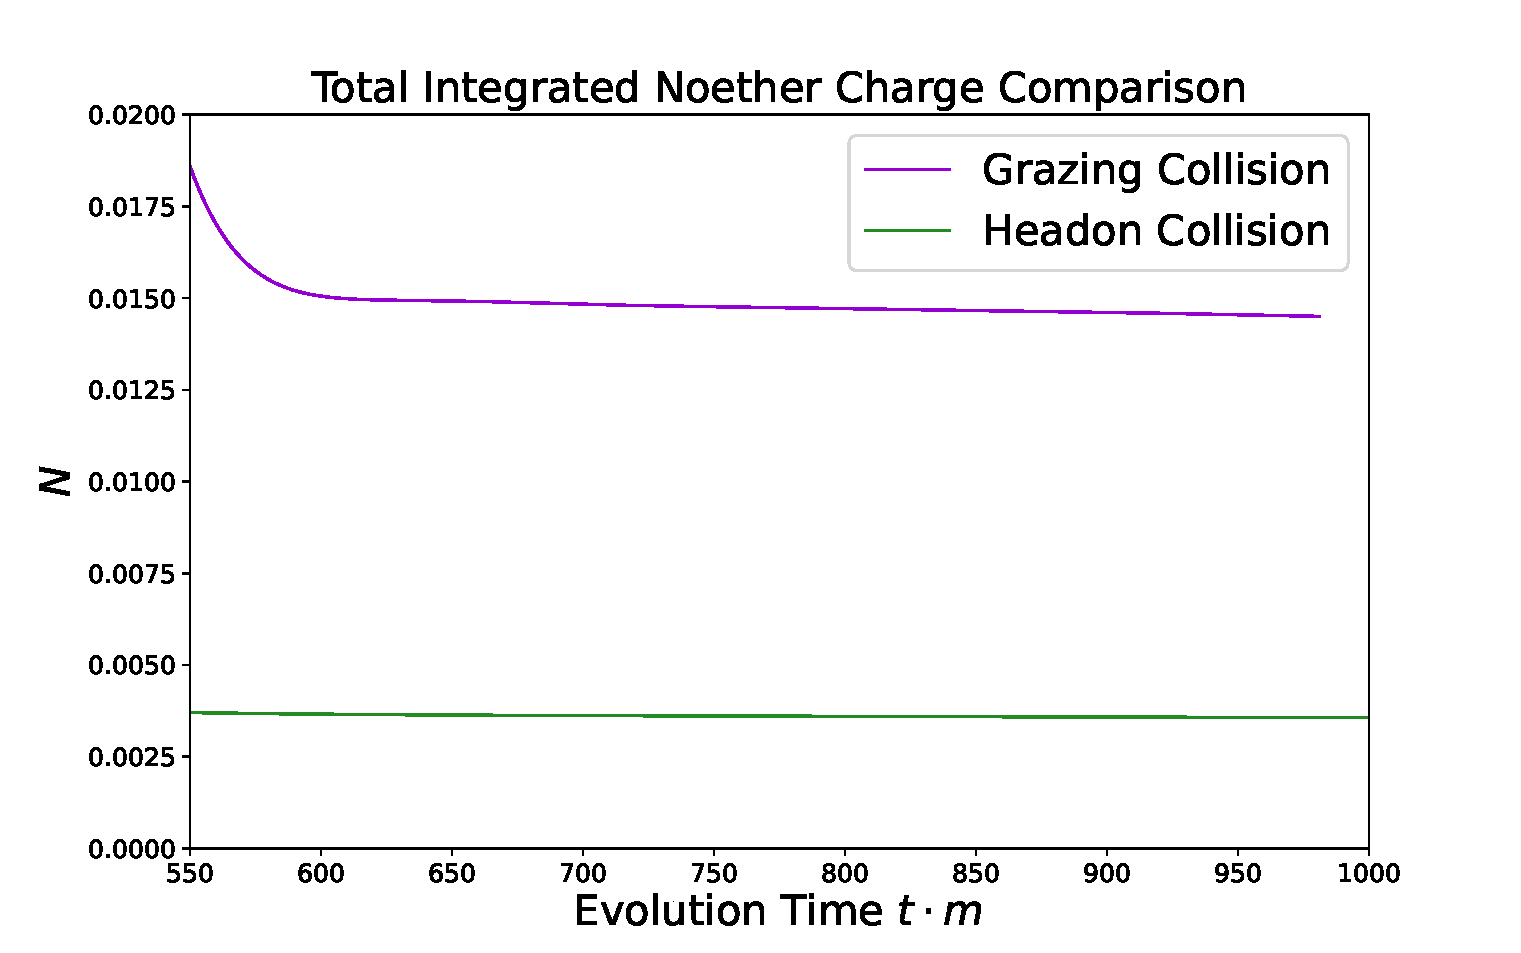
\includegraphics[width=0.45\textwidth]{data/late_time_N_nicer.pdf}}
\subfloat{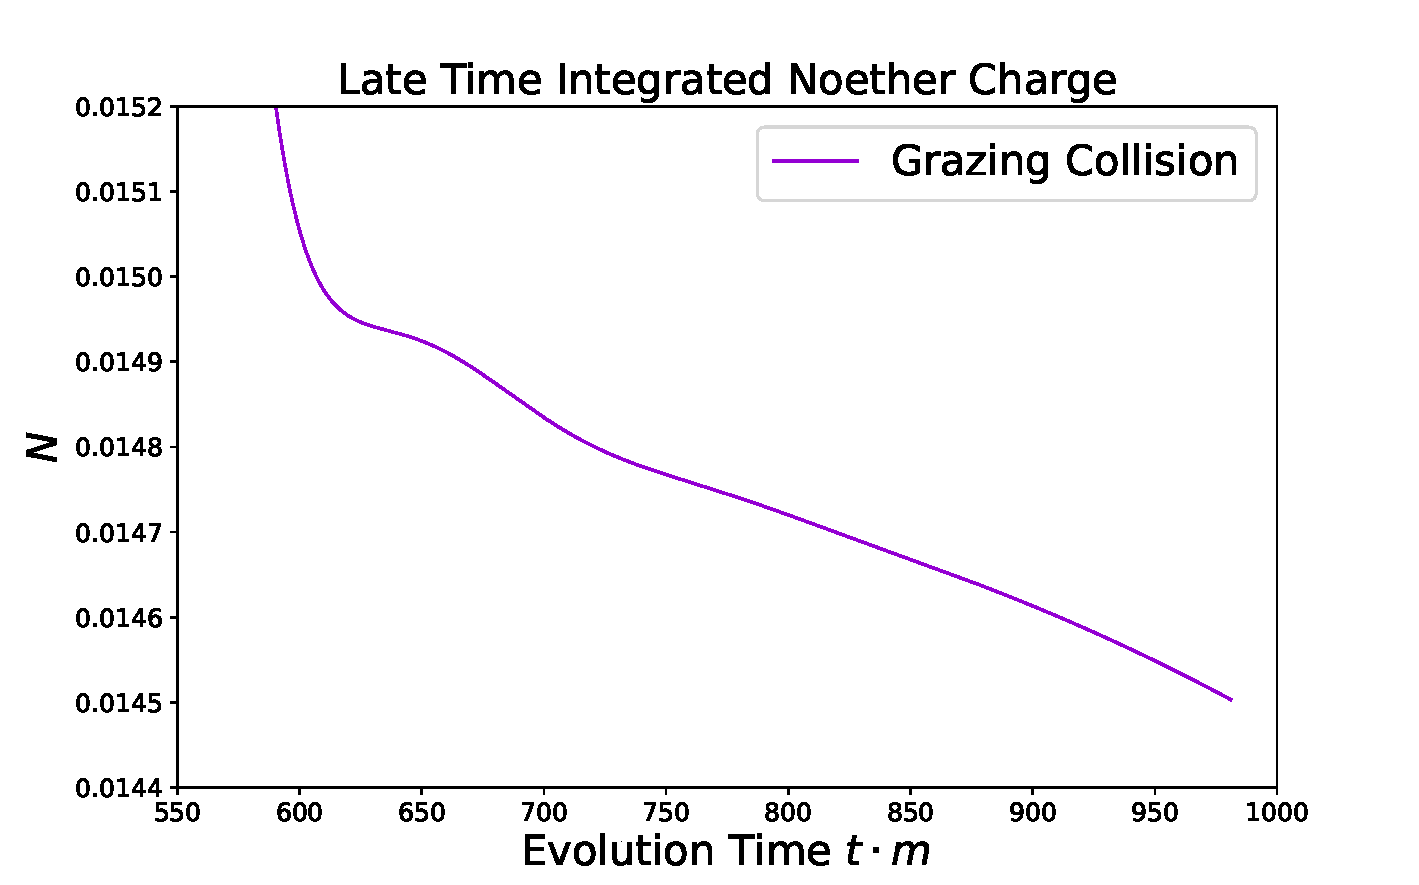
\includegraphics[width=0.45\textwidth]{data/noether_zoom_nicer.pdf}}
\label{boson:fig:fff}
\end{figure}



Figure (\ref{boson:fig:fff}) shows the late time Noether charge of the grazing and headon collisions. In contrast to the headon collision, the decay of $N$ in the grazing case is slower and reaches a value approximately $7$ times greater. Using linear extrapolation, the Noether charge of the grazing collision decays to zero at time $t \approx 12500 ~m^{-1} $ and hence the toroidal wig has an approximate lifespan of $12000~m^{-1}$.





 \begin{figure}[h!]
  \subfloat{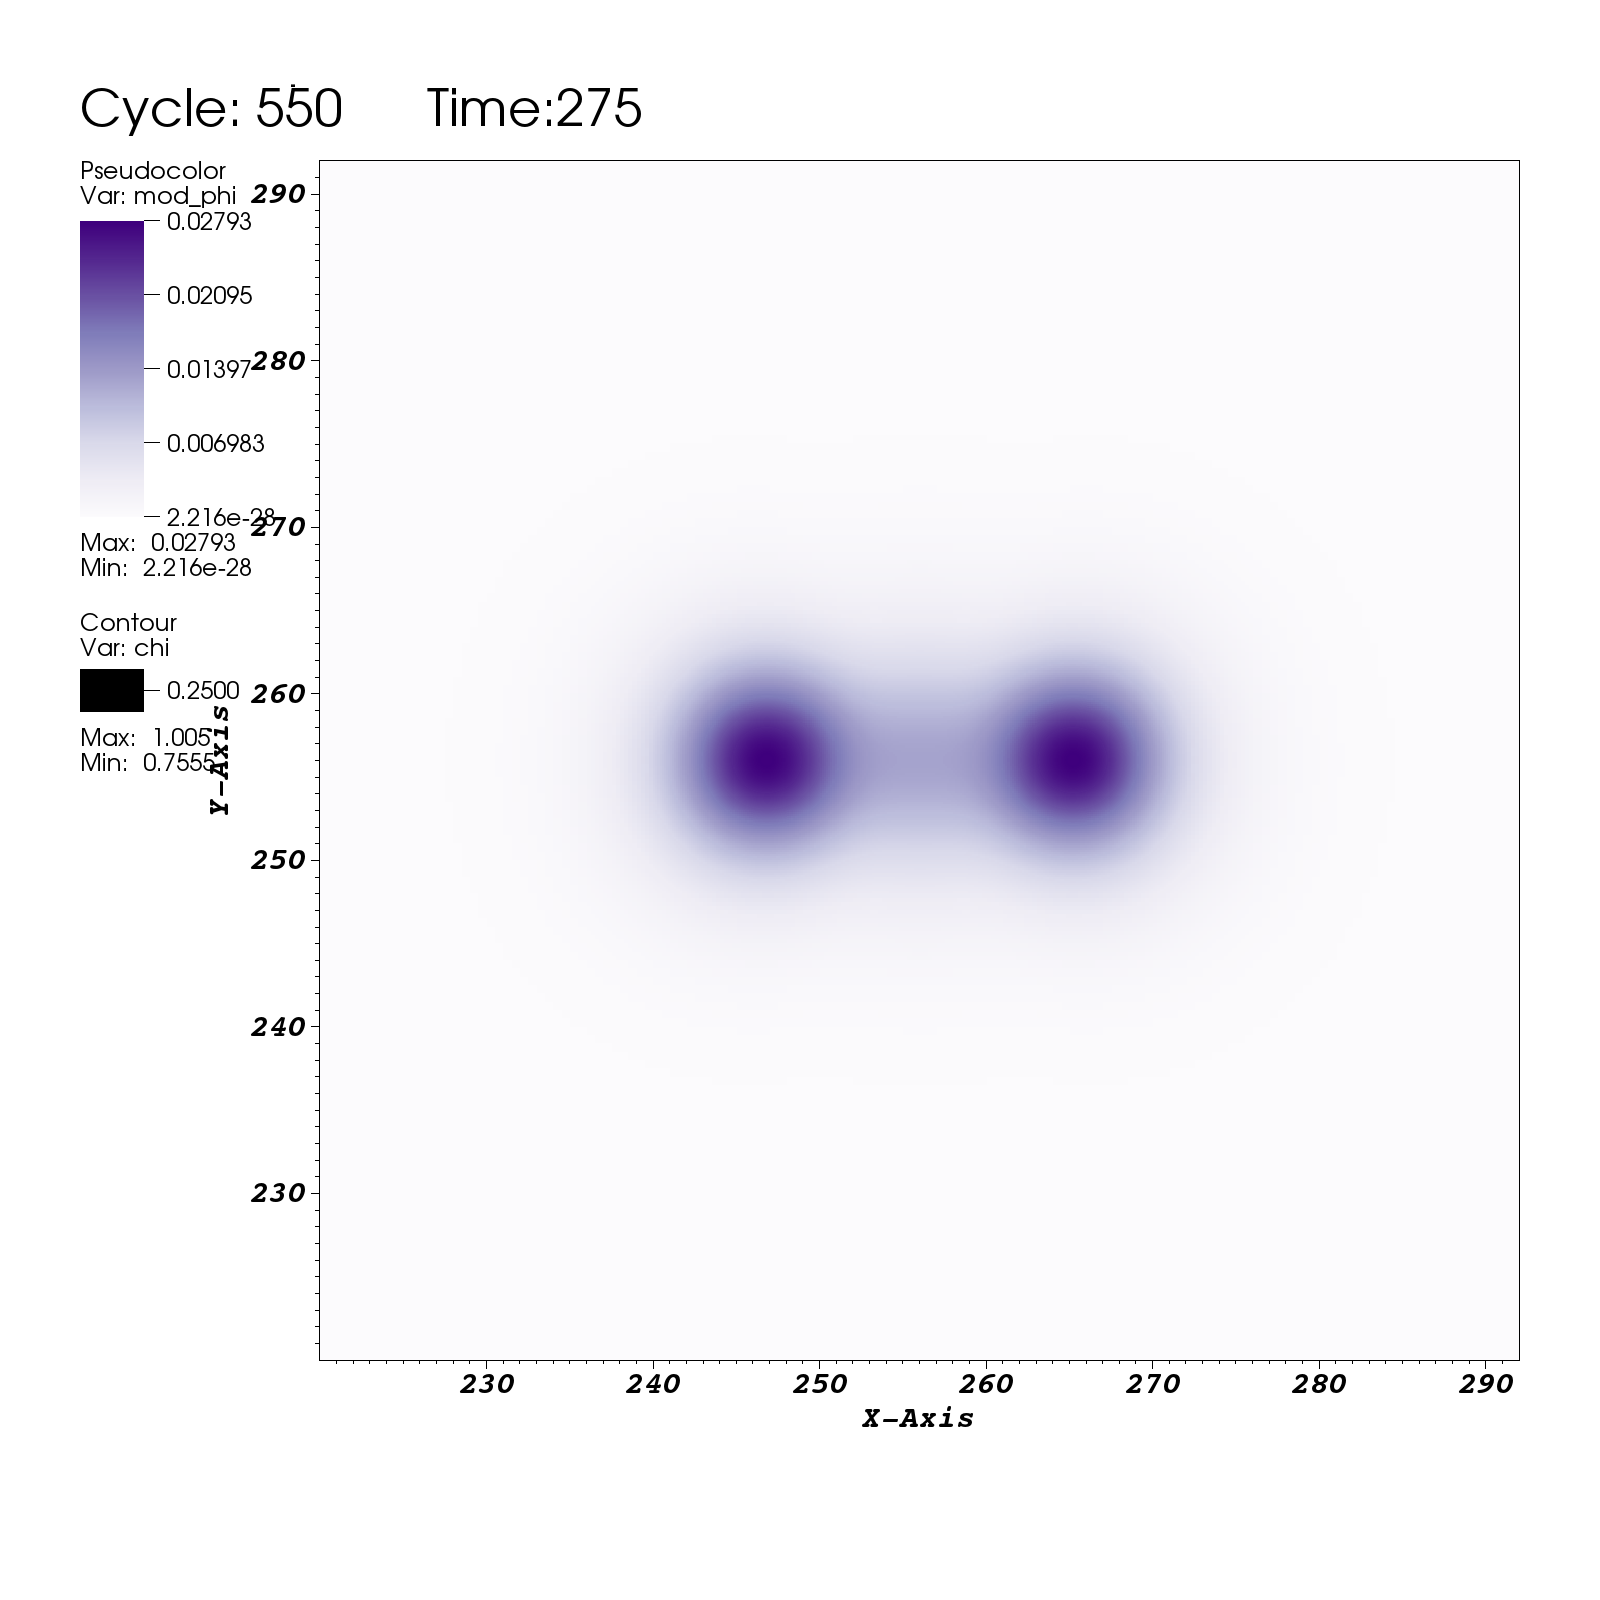
\includegraphics[width=0.50\textwidth]{modphi/headon_mod_phi0011.png}}\hfill
  \subfloat{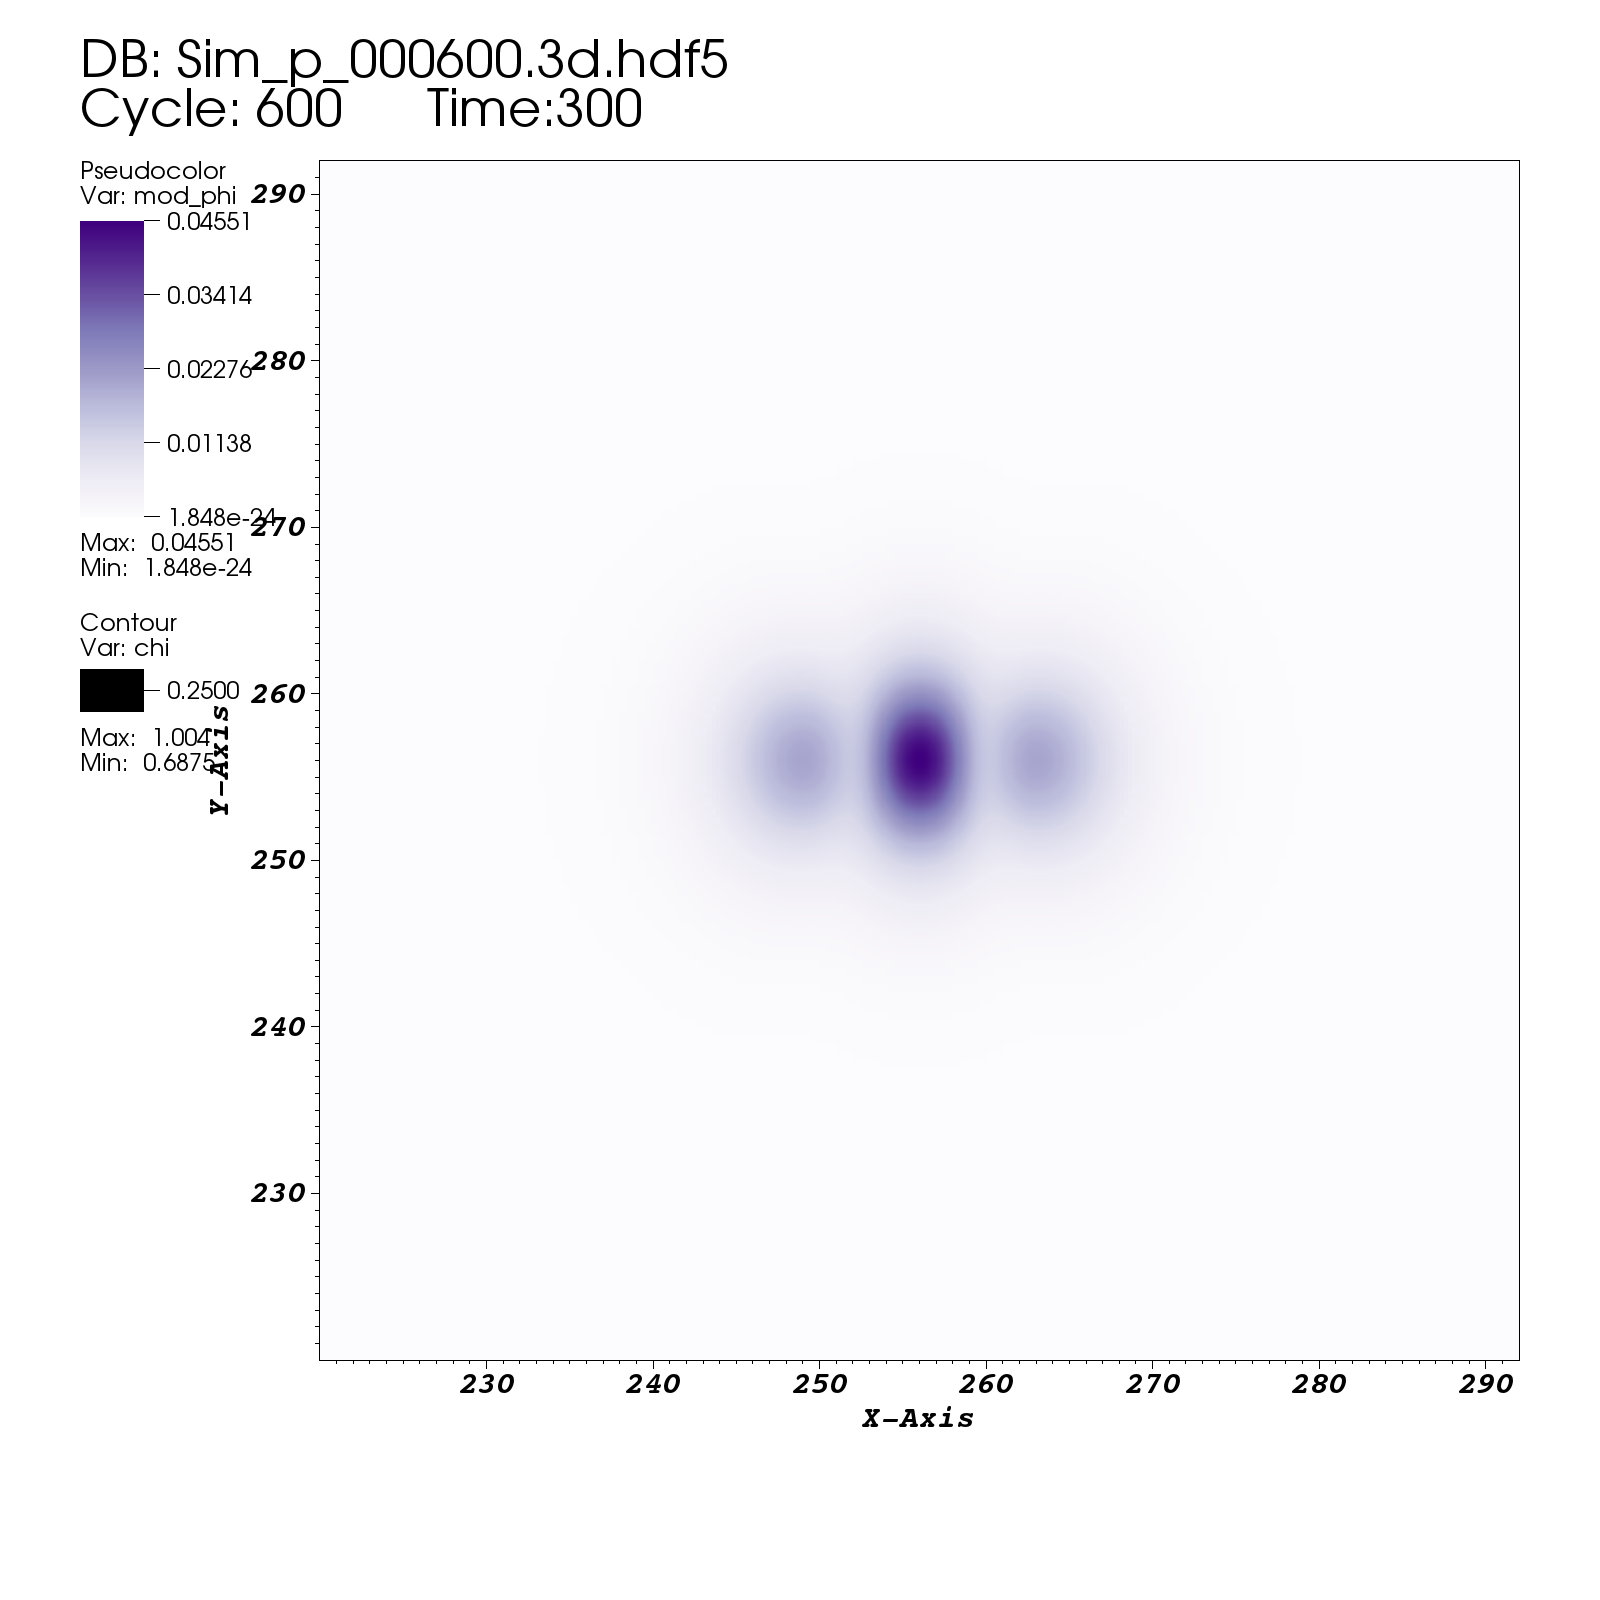
\includegraphics[width=0.50\textwidth]{modphi/headon_mod_phi0012.png}}
  \hspace{0 mm}
  \subfloat{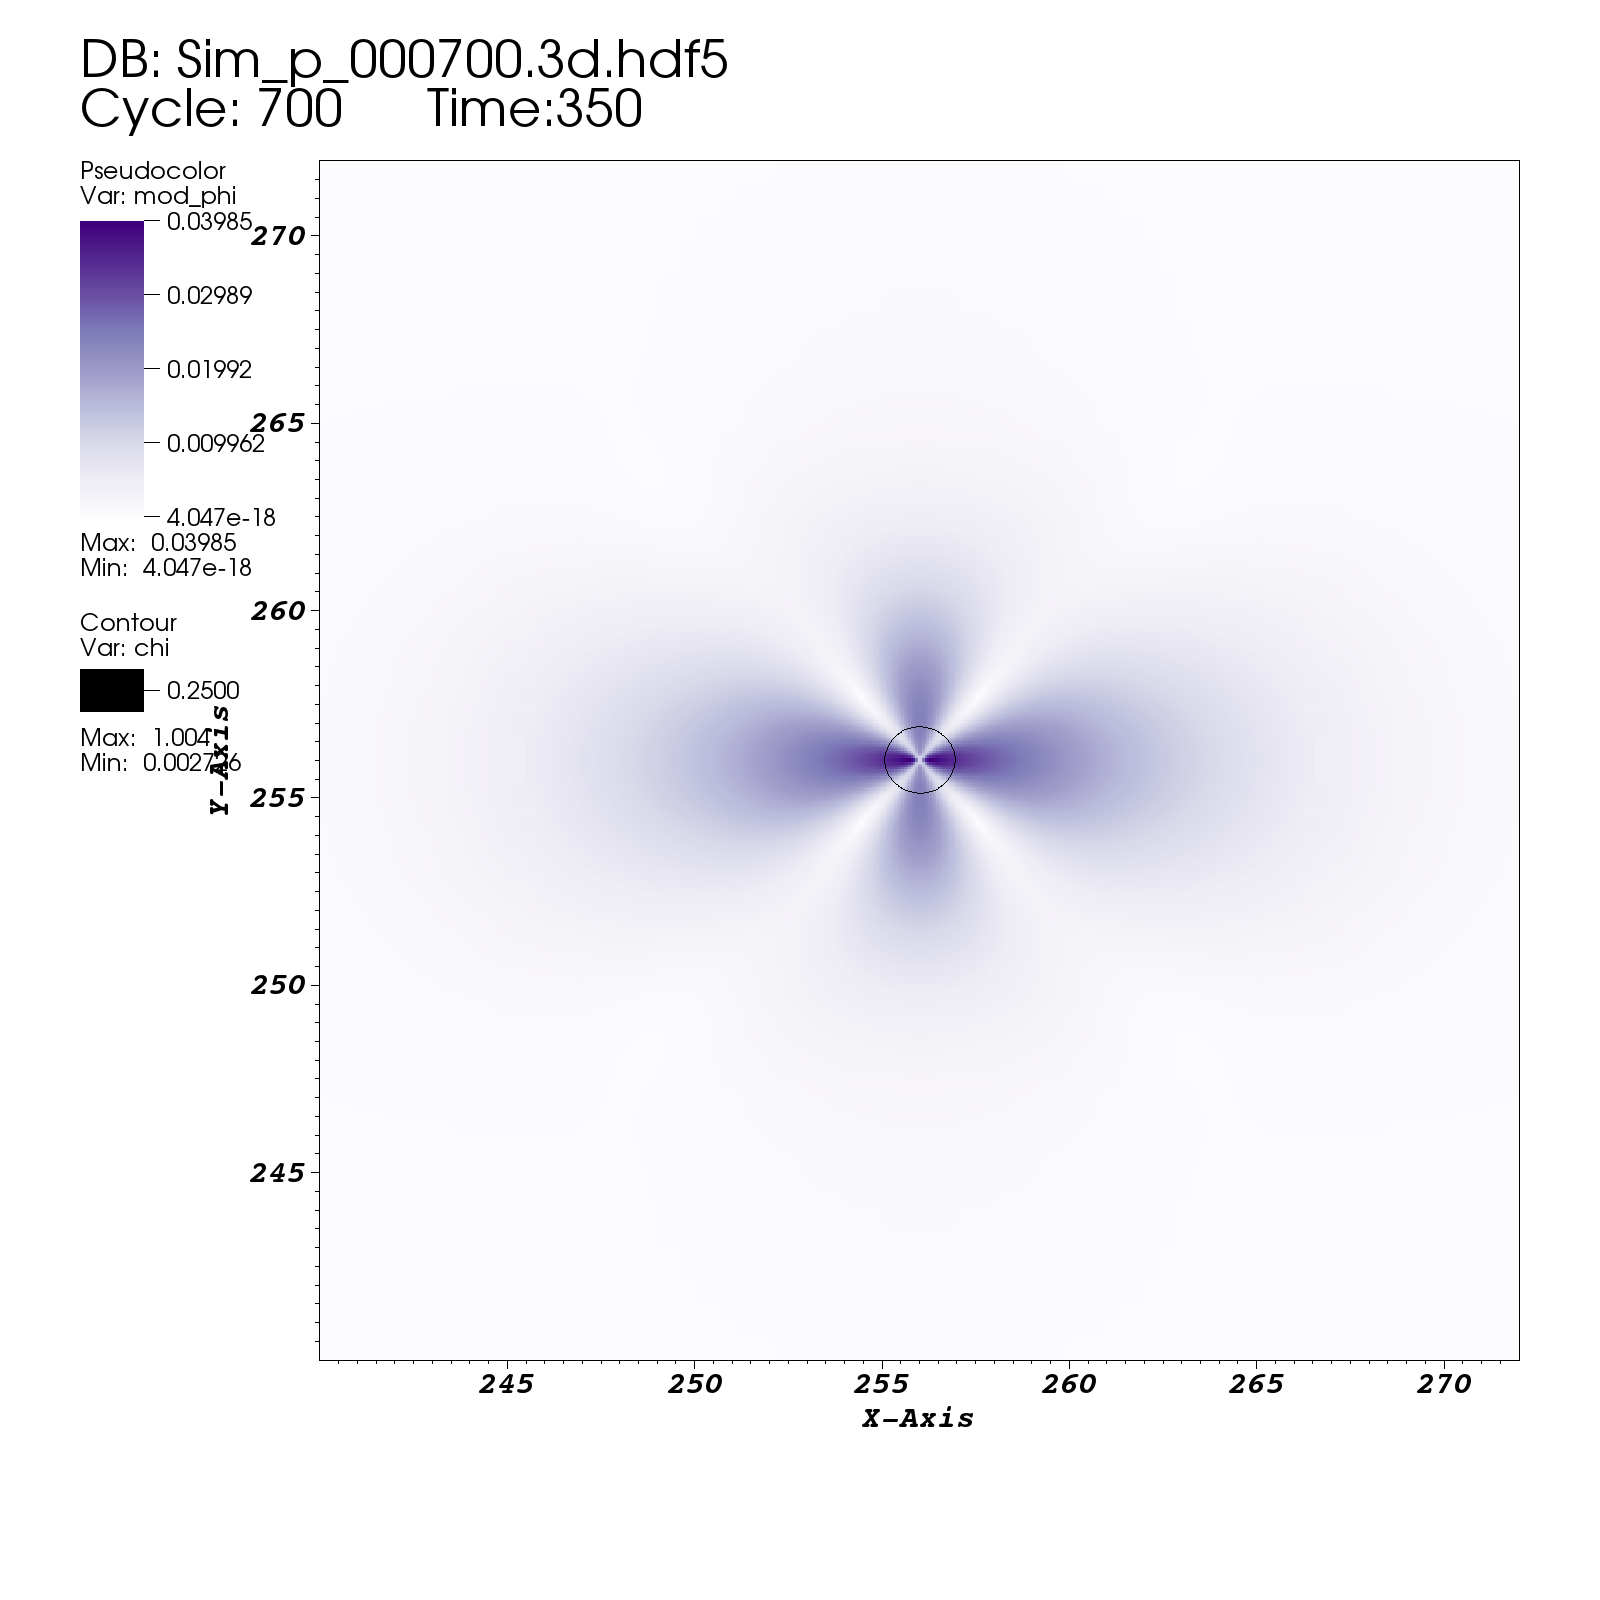
\includegraphics[width=0.50\textwidth]{modphi/headon_mod_phi0014.png}}\hfill
  \subfloat{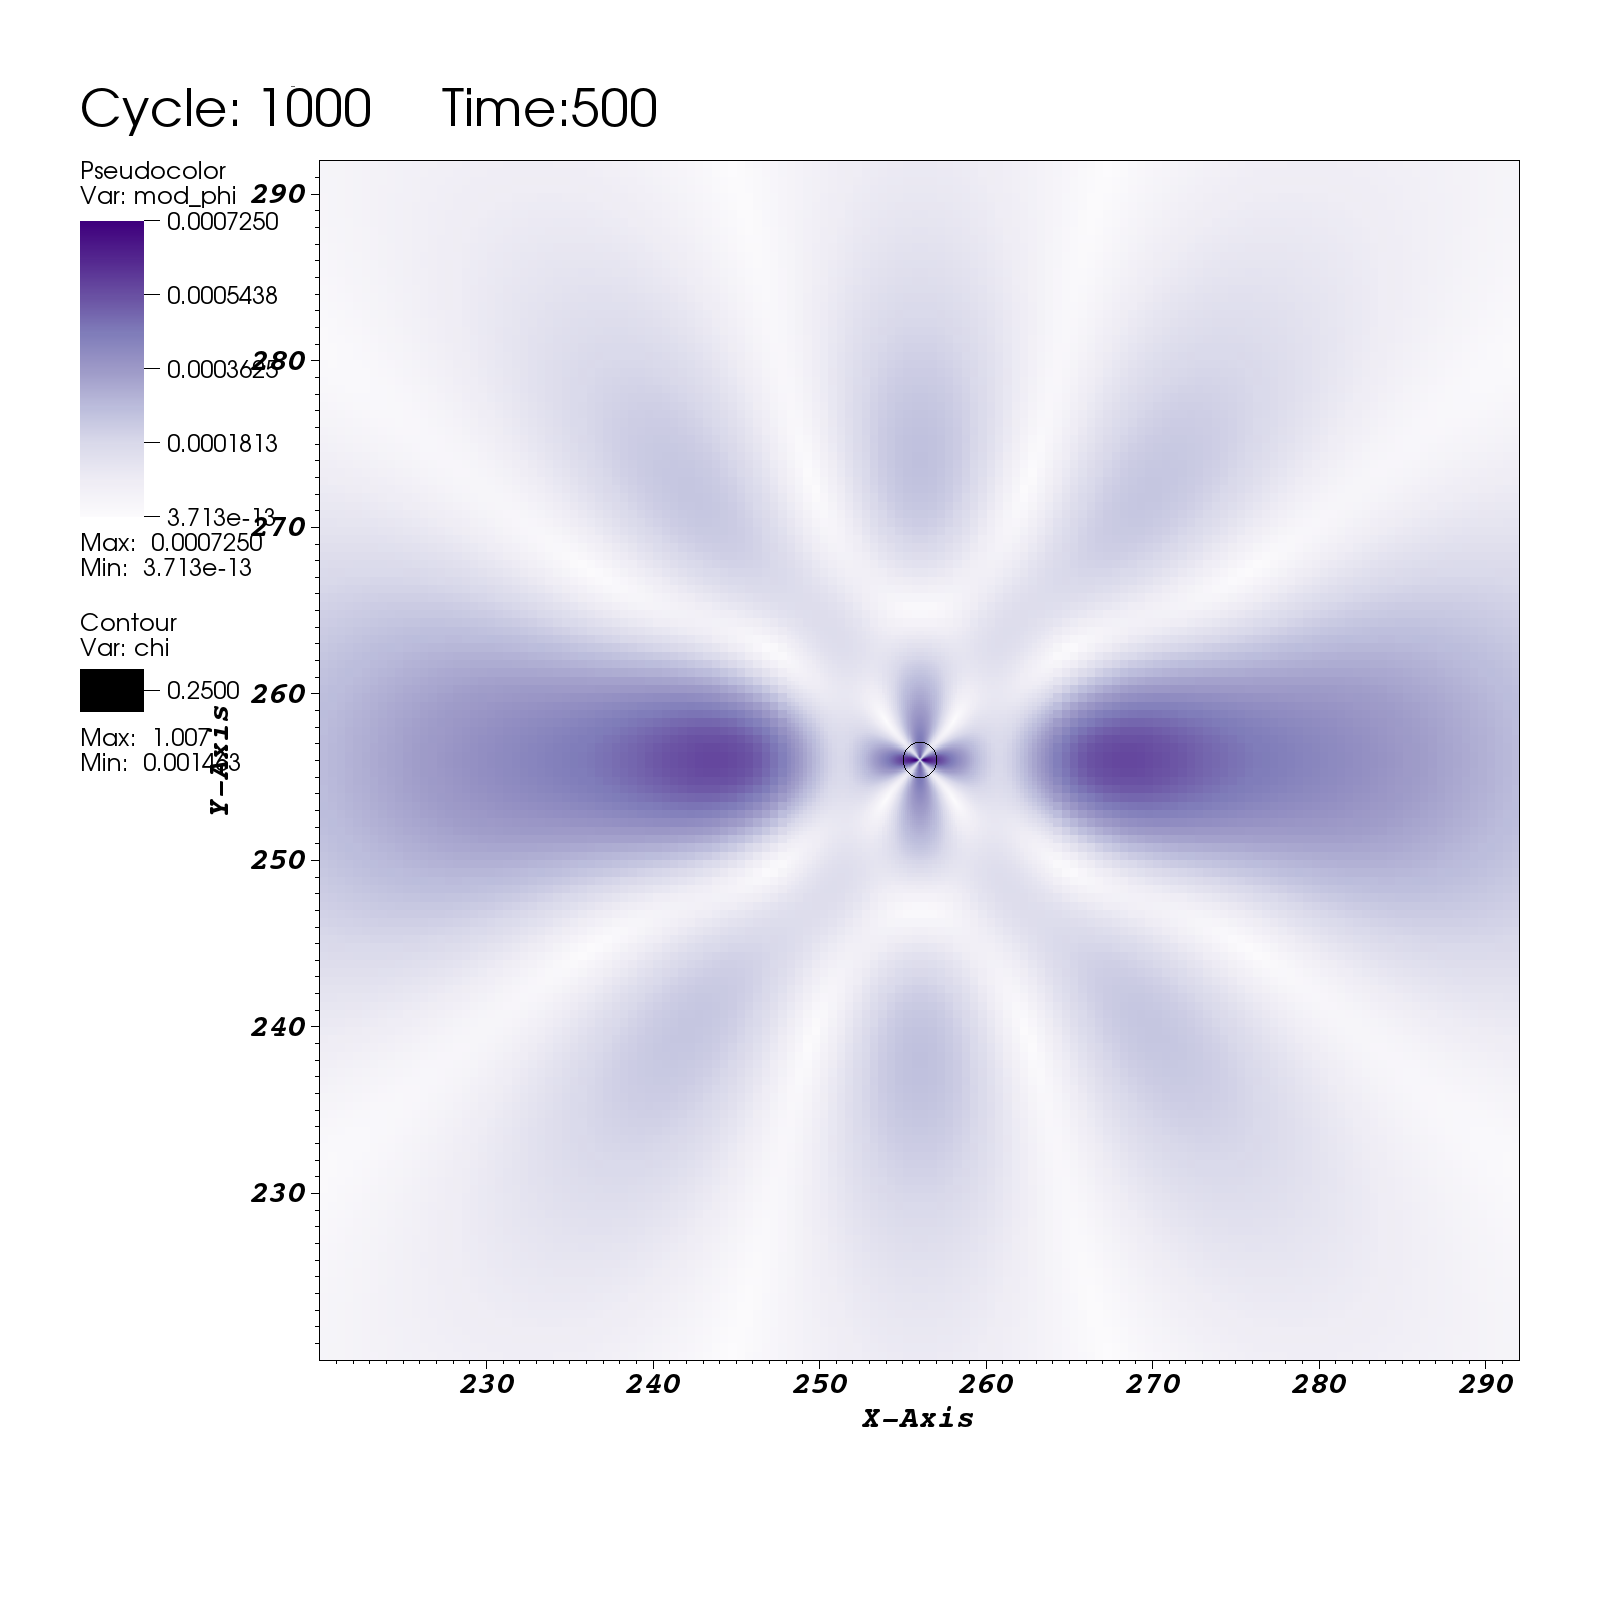
\includegraphics[width=0.50\textwidth]{modphi/headon_mod_phi0020.png}}
  \caption{Field plots of $|\vp|$ during evolution at four different times. Time $t=275~m^{-1}$ and $t=300~m^{-1}$ show snapshots momentarily before and after star collision. Time $t=350~m^{-1}$ shows the scalar field accreting into the recently formed black hole. Time $t= 500~m^{-1}$ shows the scalar field surrounding the black hole a little later; notably the amplitude is lower. Both the plots of $t=350~m^{-1}$ and $t=500~m^{-1}$ include a contour plot of $\chi=0.25$ acting as an approximate marker for the event horizon. The Newtonian estimate of collision time is $t= 287.6~m^{-1}$.}
  \label{boson:fig:ff7}
\end{figure}






\begin{figure}[h!]
\subfloat{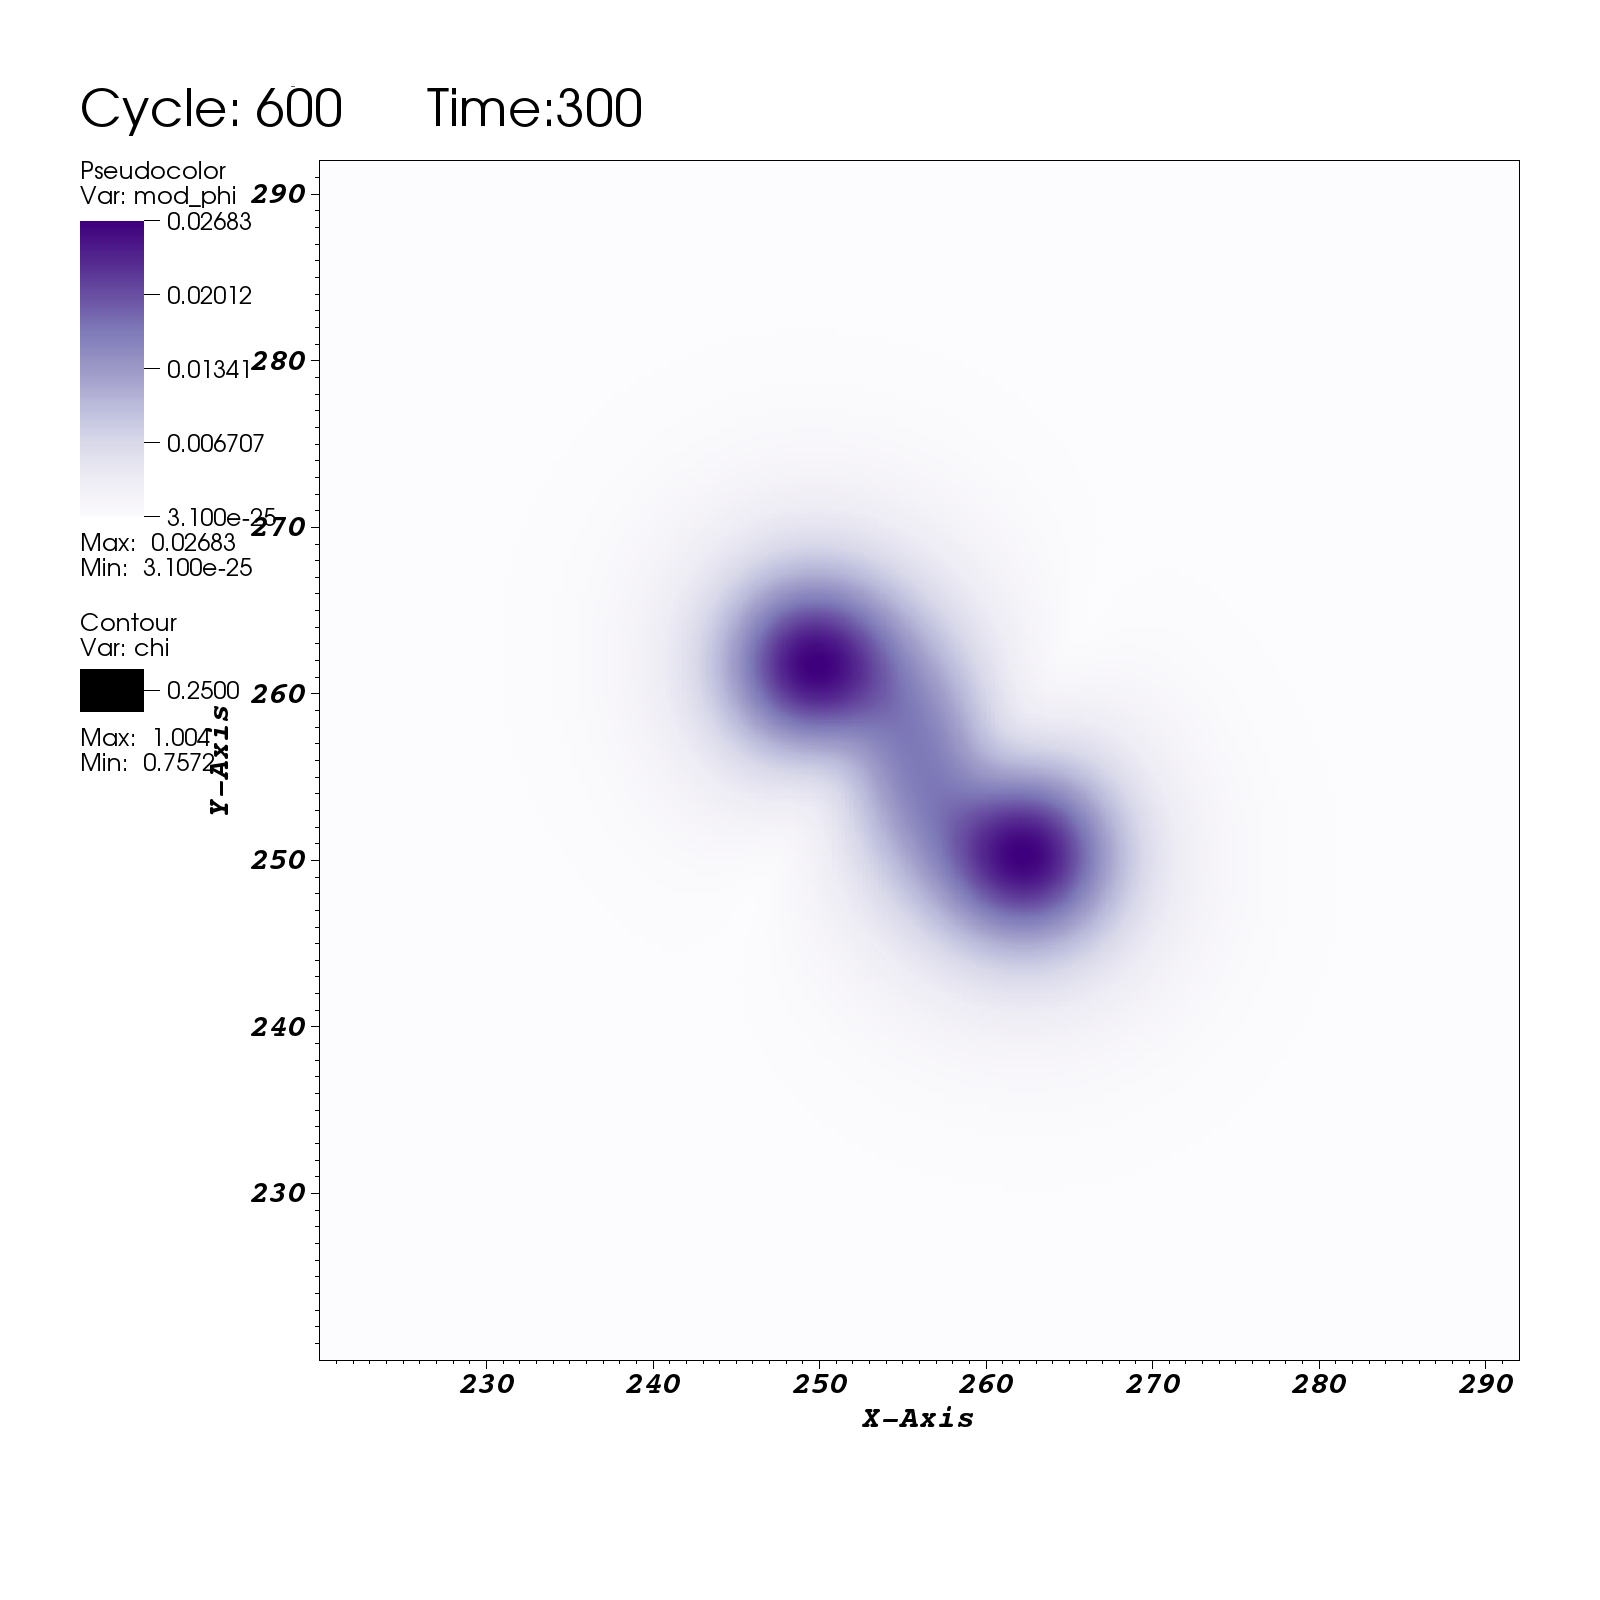
\includegraphics[width=0.5\textwidth]{modphi/graze_mod_phi0012.png}}\hfill
\subfloat{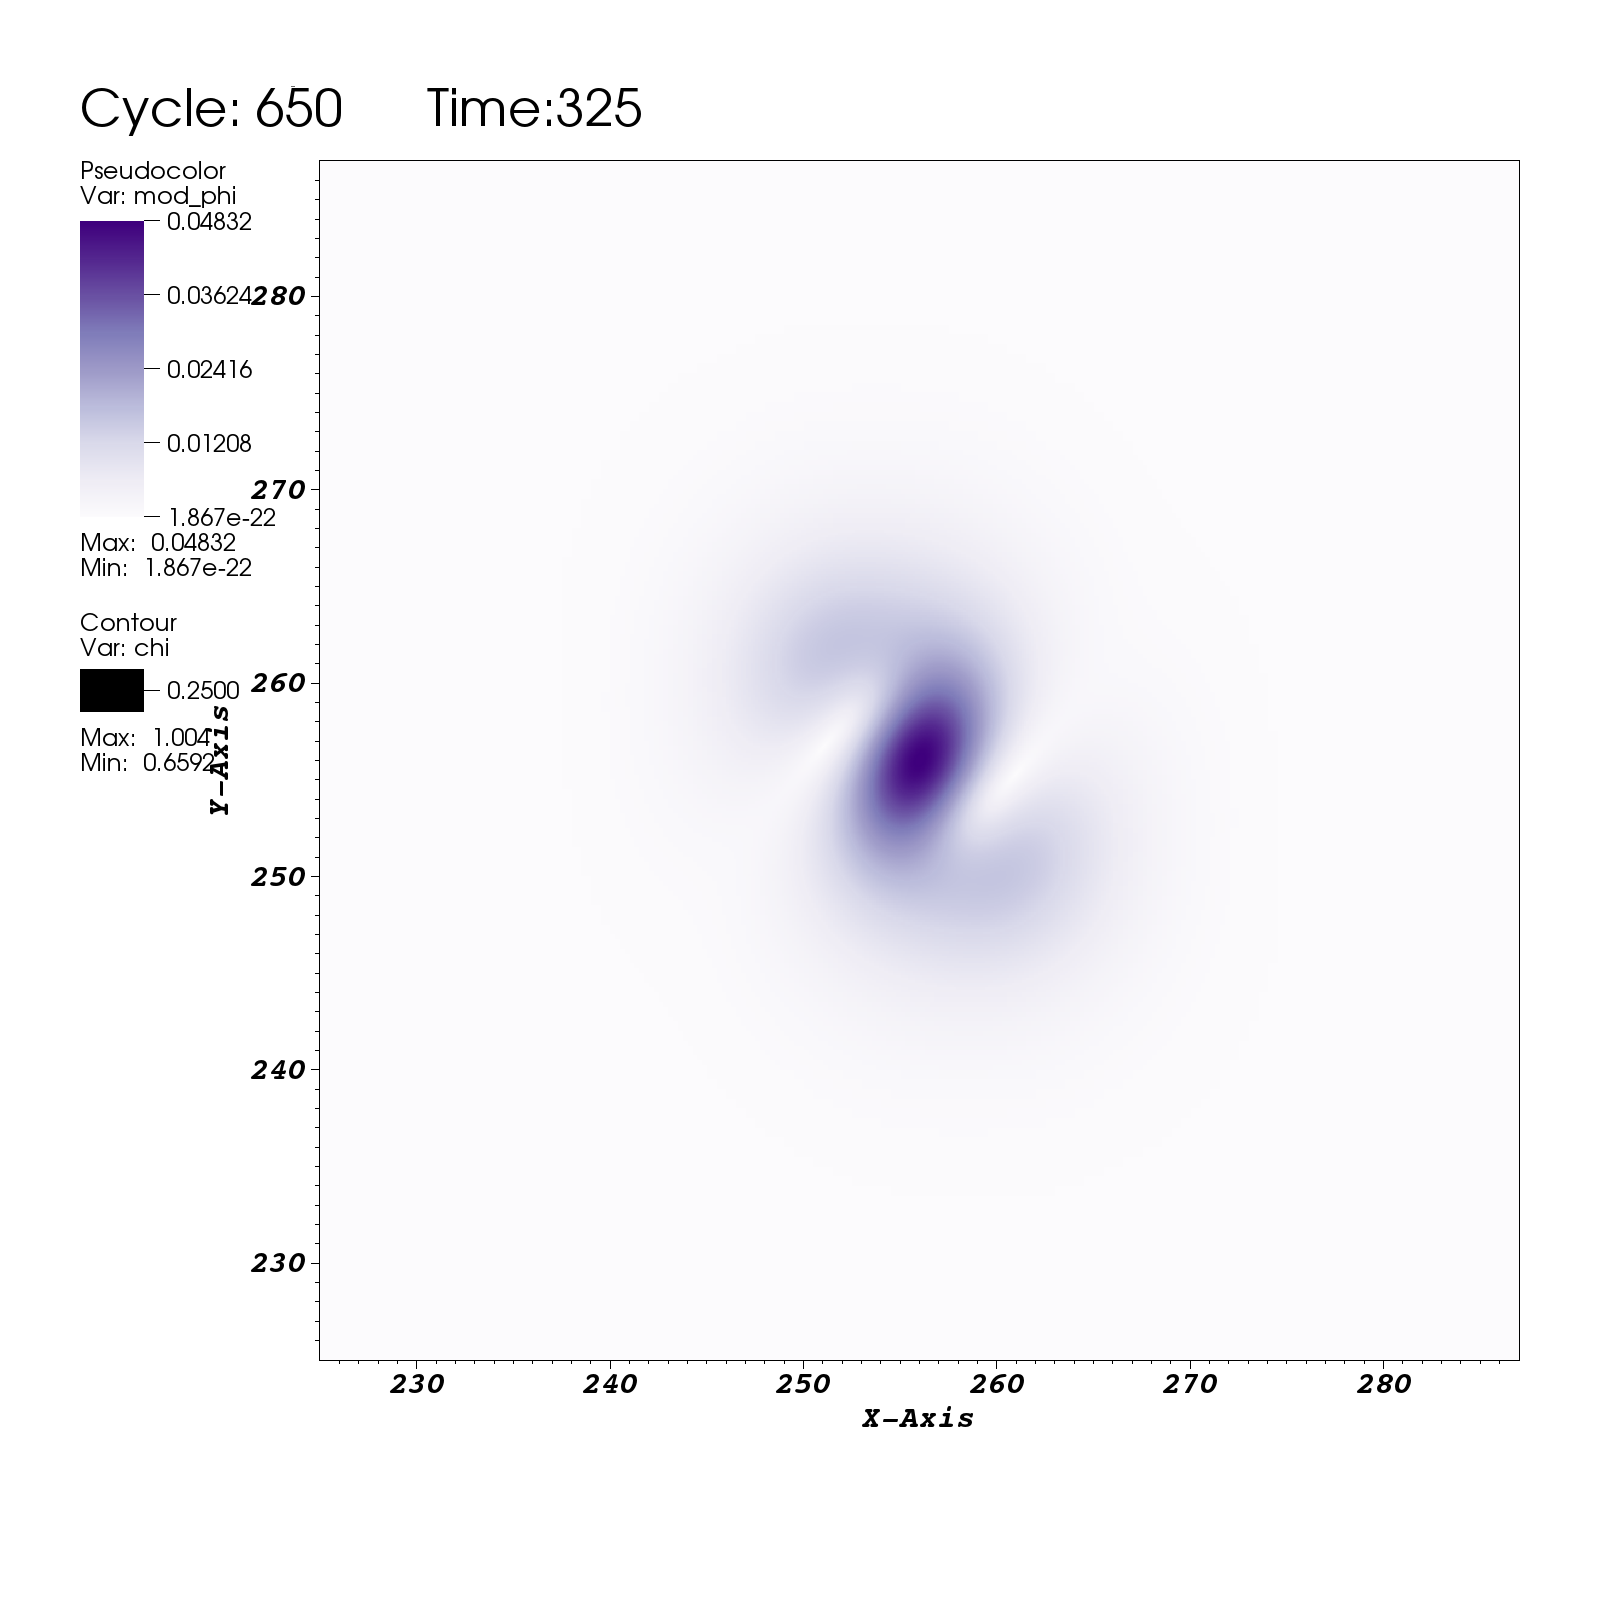
\includegraphics[width=0.5\textwidth]{modphi/graze_mod_phi0013.png}}
\hspace{0 mm}
\subfloat{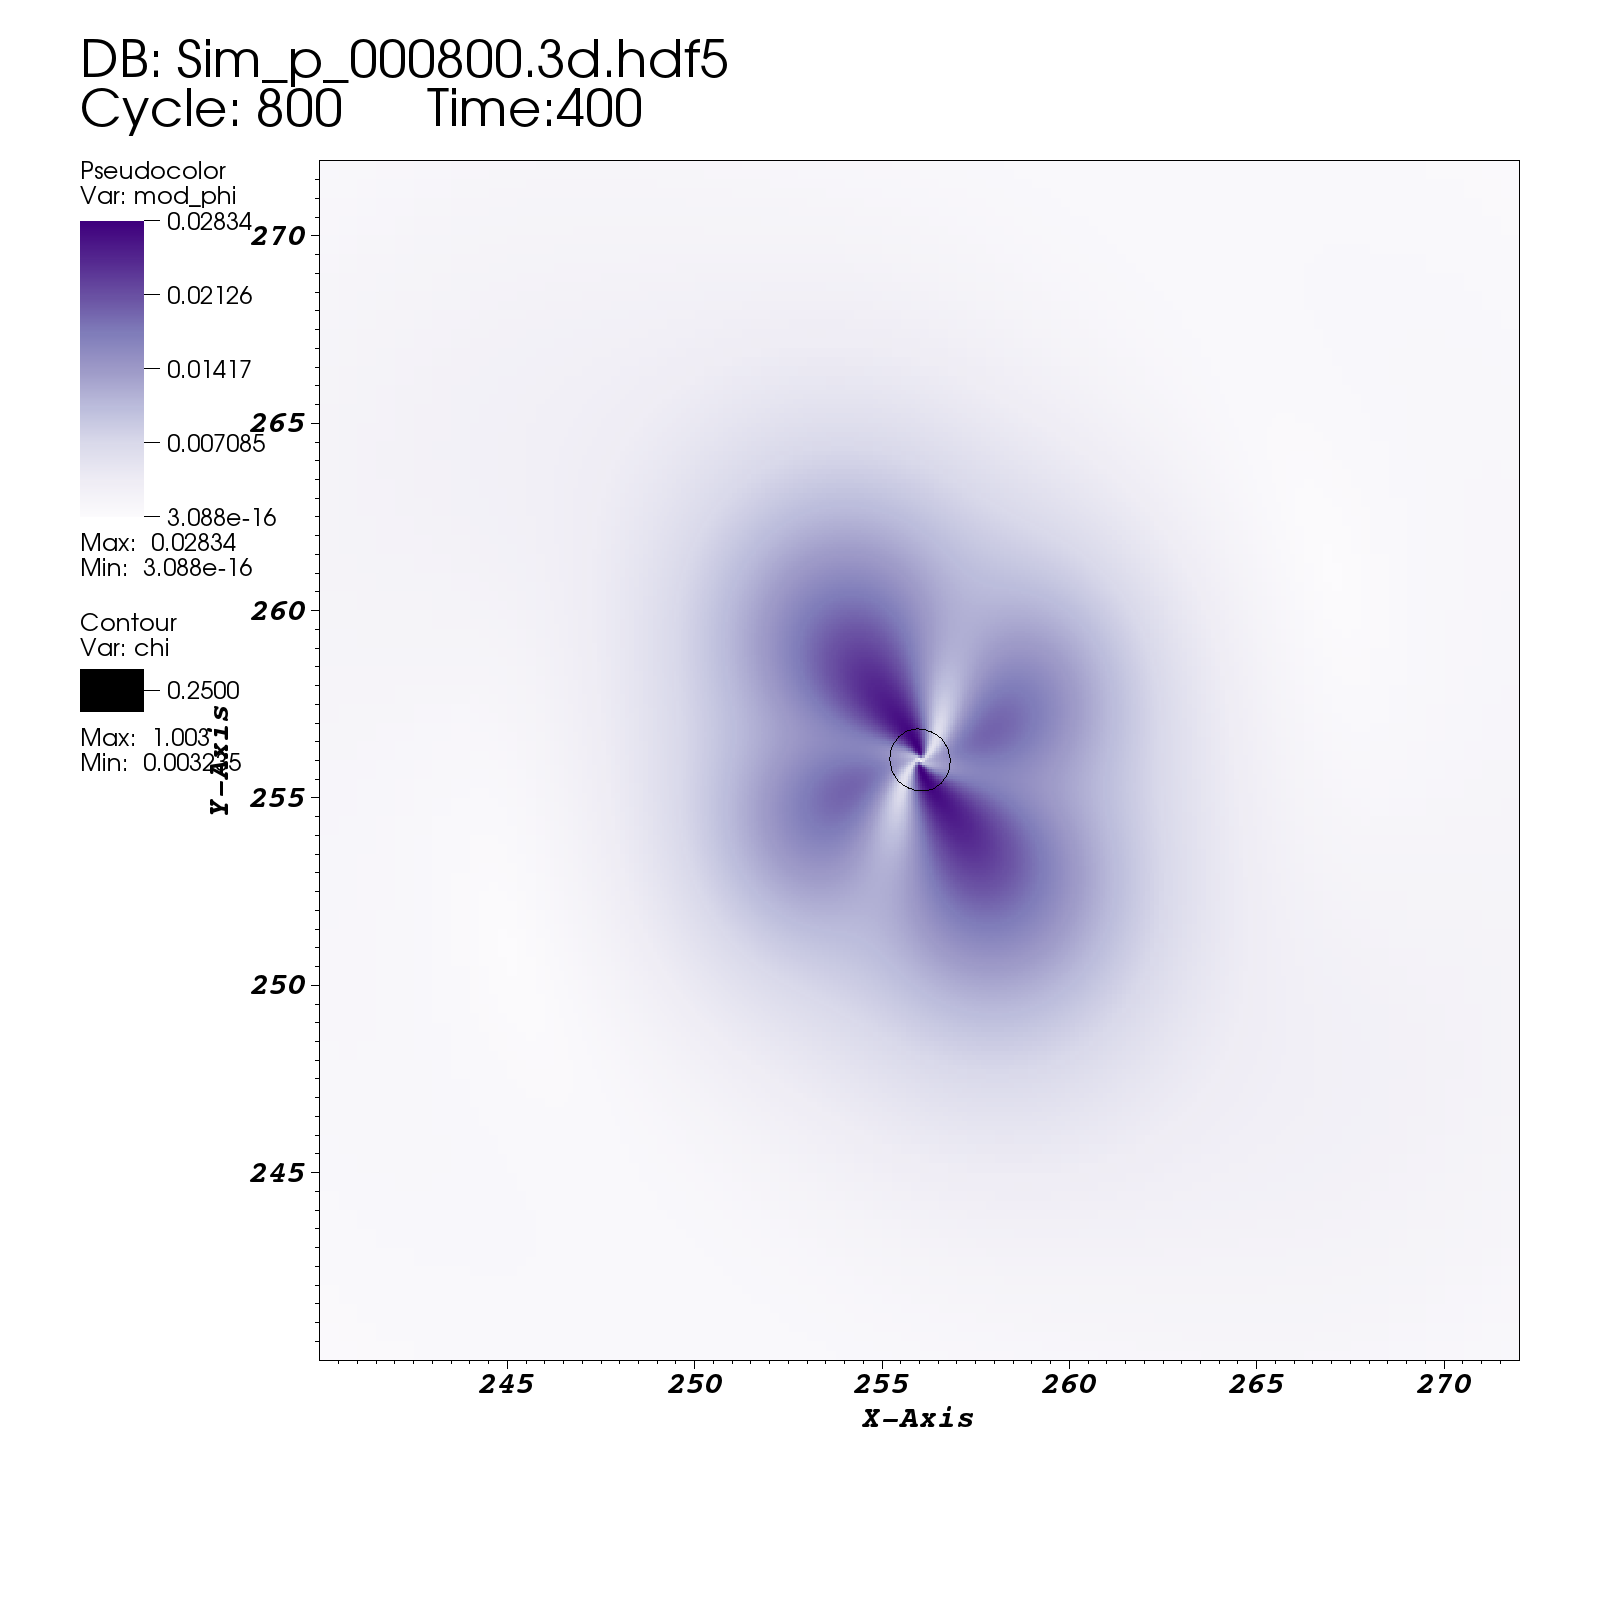
\includegraphics[width=0.5\textwidth]{modphi/graze_mod_phi0016.png}}\hfill
\subfloat{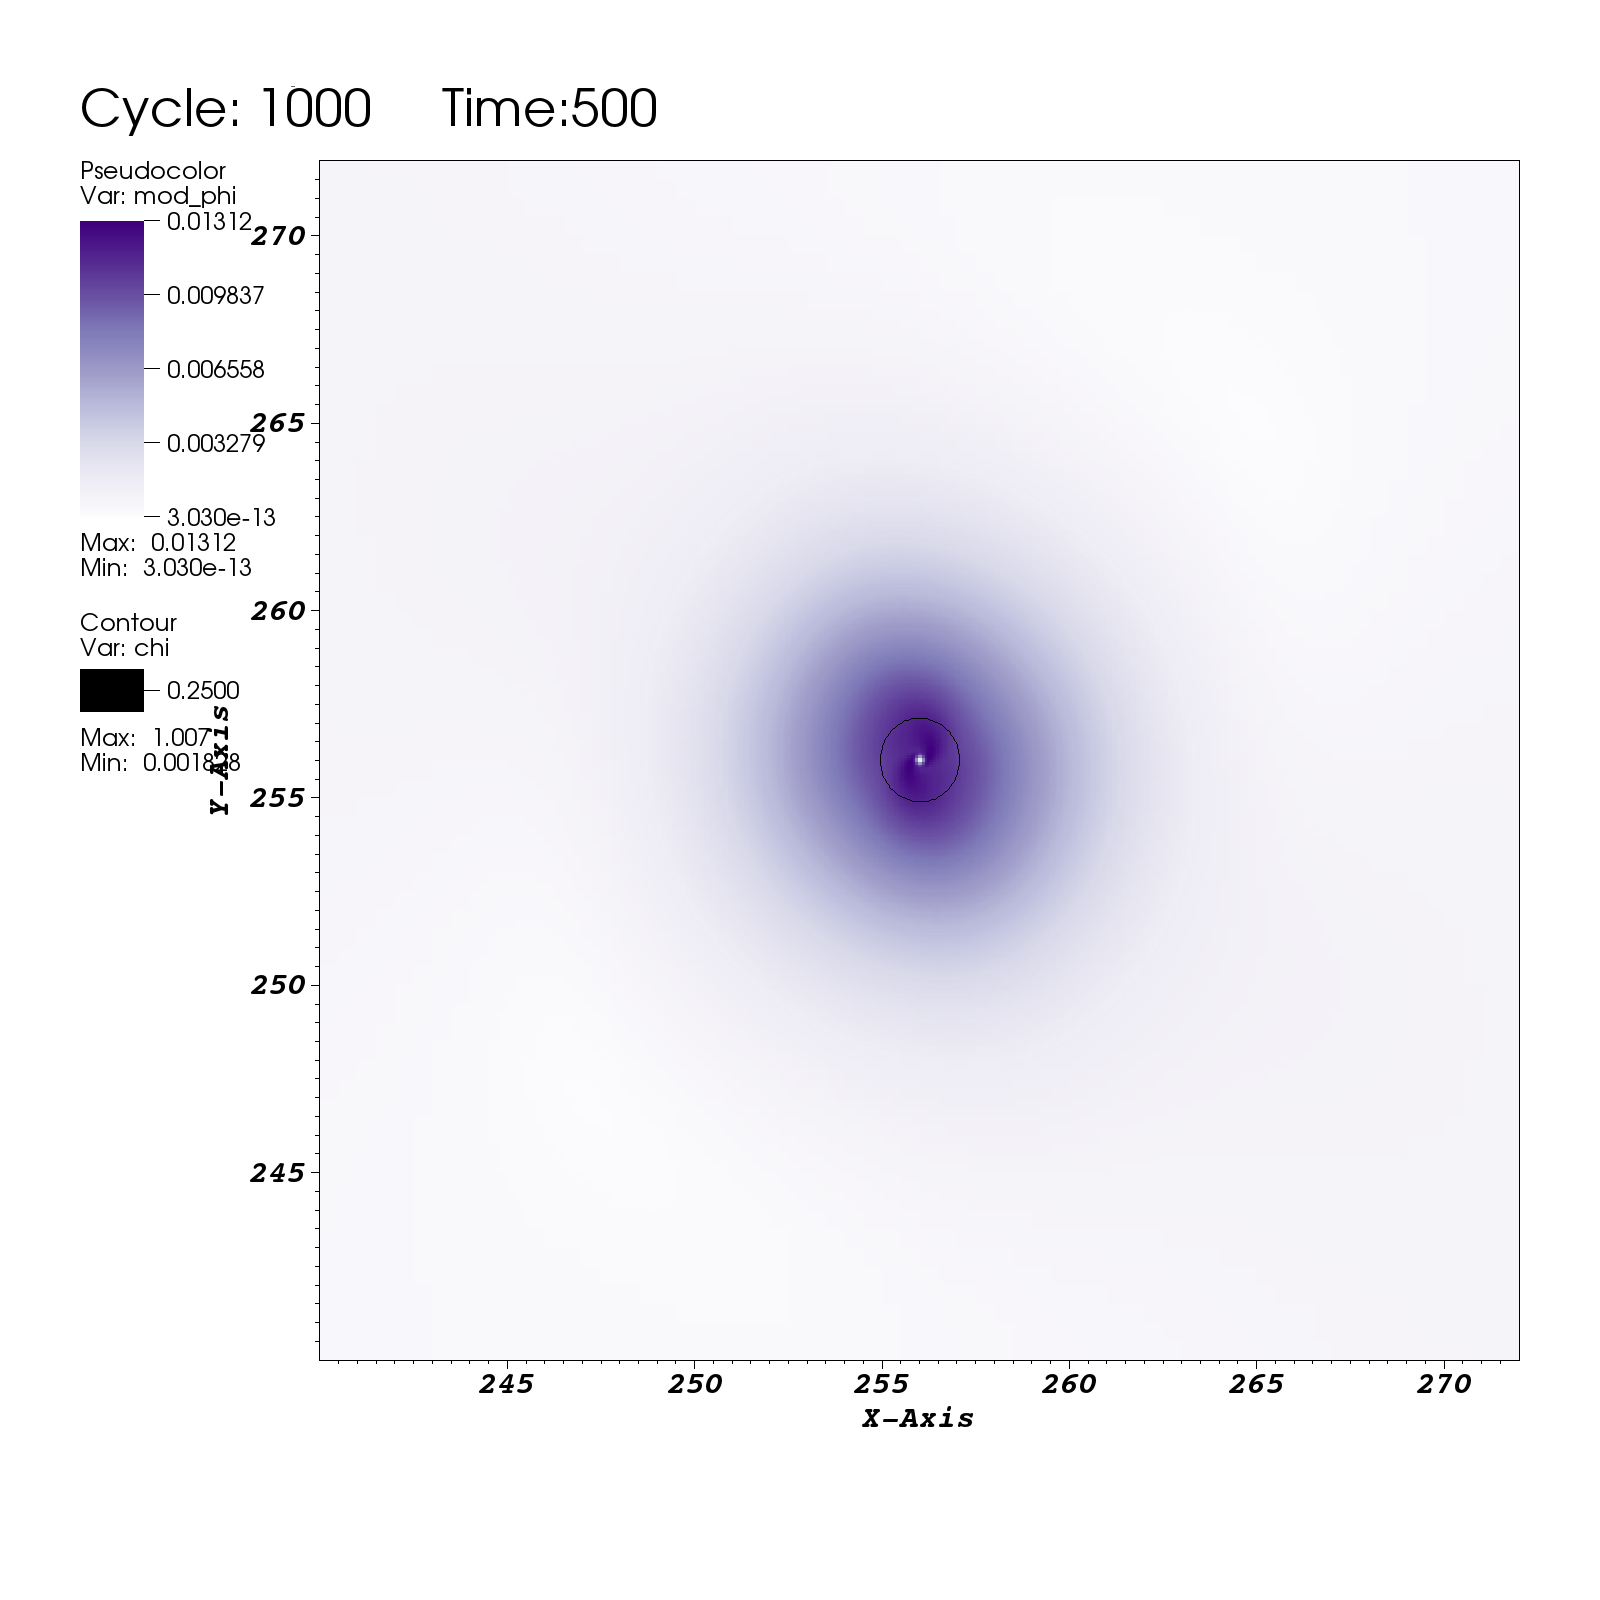
\includegraphics[width=0.5\textwidth]{modphi/graze_mod_phi0020.png}}
\caption{Field plots of $|\vp|$ during evolution at four different times for the grazing boson star collision. Time $t=300~m^{-1}$ and $t=325~m^{-1}$ show snapshots momentarily before and after the collision. The Newtonian estimate of collision time is $t= 315.8~m^{-1}$. Time $t=400~m^{-1}$ shows the scalar field accreting into the recently formed black hole. Time $t= 500~m^{-1}$ shows the scalar field surrounding the black hole a little later; here this is called a {\it toroidal wig}. Both the plots of $t=400~m^{-1}$ and $t=500~m^{-1}$ display a contour plot of $\chi=0.25$ acting as an approximate marker for the event horizon. }
\label{boson:fig:ff10}
\end{figure}



%BLACKHOLESBLACKHOLESBLACKHOLESBLACKHOLESBLACKHOLESBLACKHOLESBLACKHOLESBLACKHOLESBLACKHOLESBLACKHOLESBLACKHOLESBLACKHOLESBLACKHOLESBLACKHOLESBLACKHOLESBLACKHOLESBLACKHOLESBLACKHOLESBLACKHOLESBLACKHOLESBLACKHOLESBLACKHOLESBLACKHOLESBLACKHOLESBLACKHOLESBLACKHOLESBLACKHOLESBLACKHOLESBLACKHOLESBLACKHOLESBLACKHOLESBLACKHOLESBLACKHOLESBLACKHOLESBLACKHOLESBLACKHOLESBLACKHOLESBLACKHOLESBLACKHOLESBLACKHOLESBLACKHOLESBLACKHOLESBLACKHOLESBLACKHOLESBLACKHOLESBLACKHOLESBLACKHOLESBLACKHOLESBLACKHOLESBLACKHOLESBLACKHOLESBLACKHOLESBLACKHOLESBLACKHOLESBLACKHOLESBLACKHOLESBLACKHOLESBLACKHOLESBLACKHOLESBLACKHOLESBLACKHOLESBLACKHOLESBLACKHOLESBLACKHOLES


% \subsection{Collisions of Boson Stars with Black Holes} \label{grchombo:sec:bsbhcollisions}

% Here the headon and grazing collisions of a boson star with a black hole are presented. The superposition scheme is given in section \ref{grchombo:sec:superposition}. Similarly to the previous section on the collision of two identical stars, the star and black hole mass are identical, each with an ADM mass $M=0.532(7)$. The black hole and star are placed at positions $\pm\{40,0,0\}$ in the headon case and $\pm\{40,8,0\}$ in the grazing case and are boosted together with respective velocities $\mp\{0.1,0,0\}$ corresponding to a rapidity of $\psi=0.1003353$ (4 s.f.). The simulations have a physical domain size $L=512$ with $N=256$ gridpoints on AMR level zero, this gives a coarse grid resolution of $\Delta x = 2$. There are up to five extra AMR levels giving a finest grid resolution of $\Delta x = 16$.

% \subsubsection{Headon Collision}
%  \begin{figure}[h!]
%   \caption{Left: Maximum of $|\vp|$ during evolution, Right: Total integrated Noether charge $N$.}
%   \centering
%   \subfloat{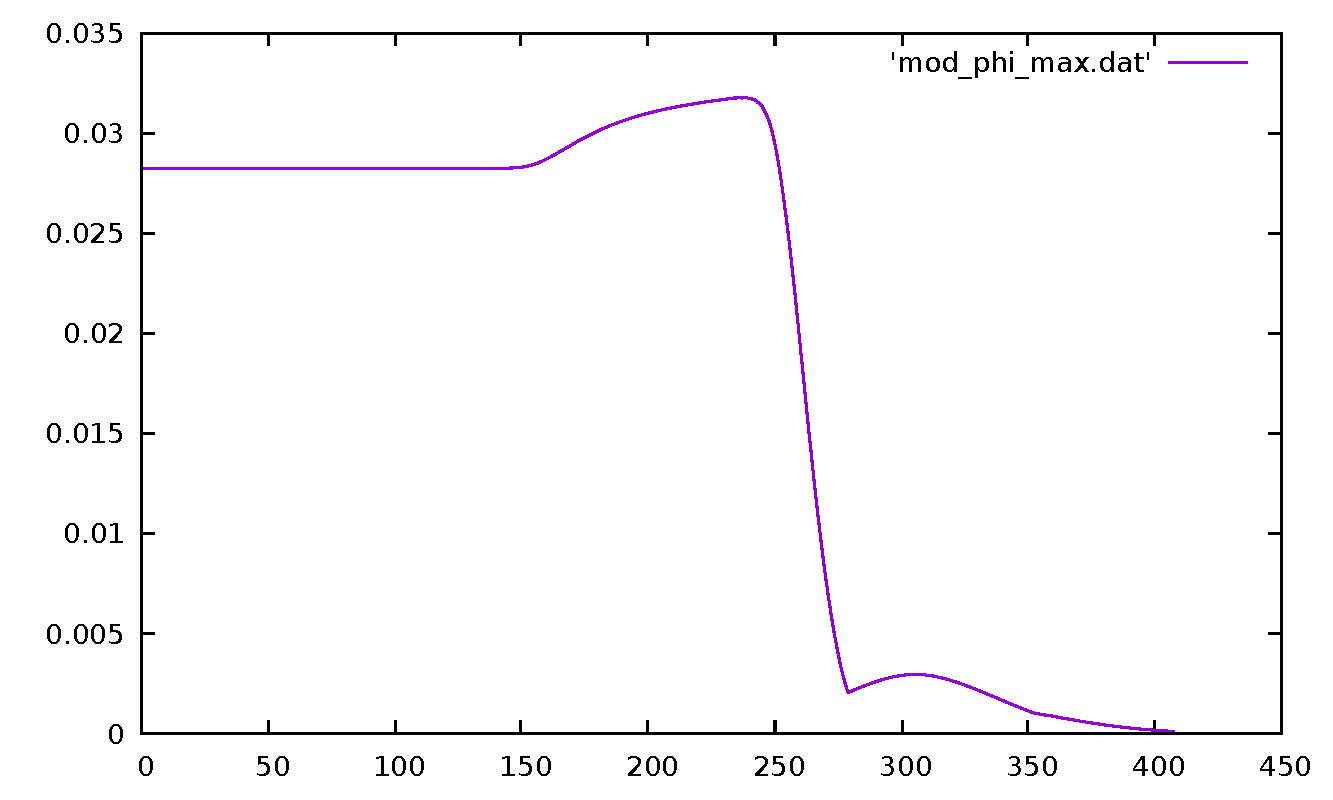
\includegraphics[width=0.5\textwidth]{data/headon_bhbs_modphi.pdf}\label{boson:fig:f12}}
%   \hfill
%   \subfloat{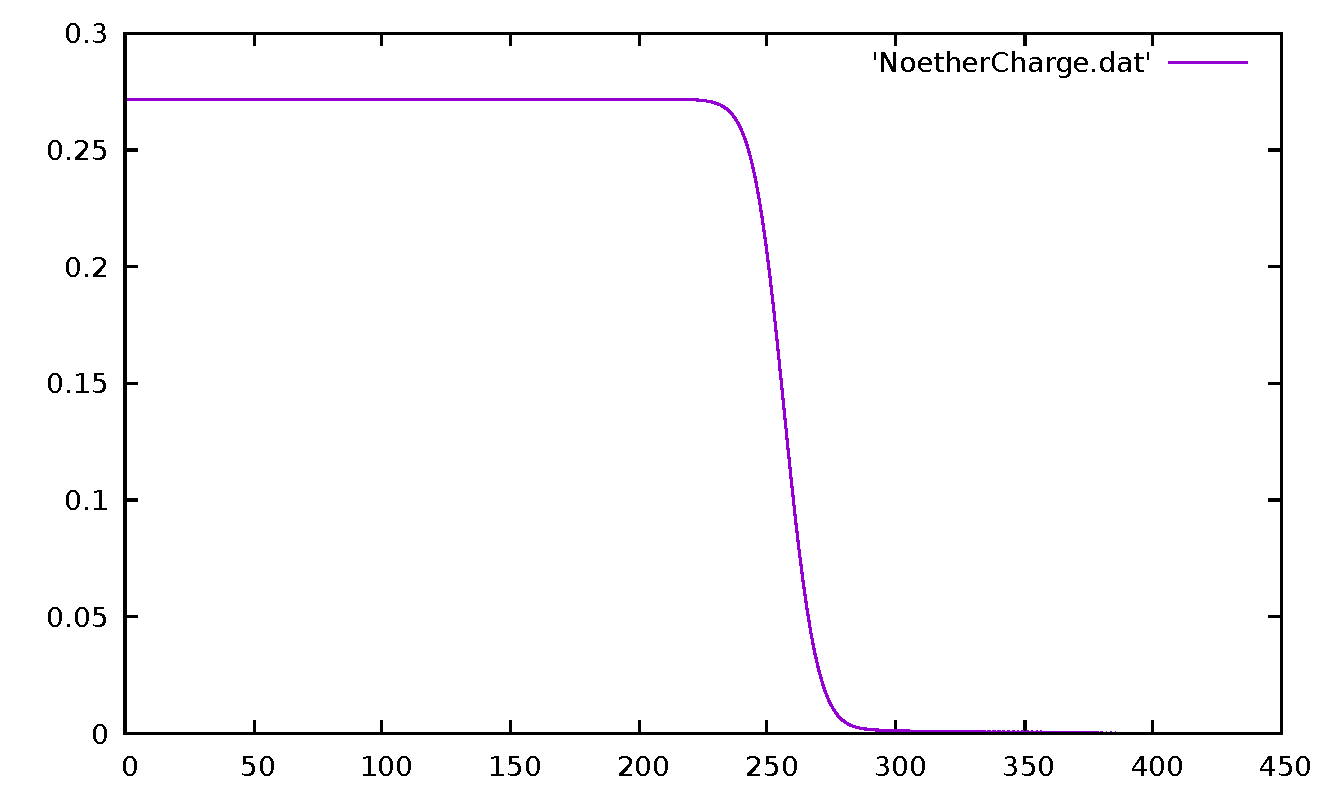
\includegraphics[width=0.5\textwidth]{data/headon_bhbs_n.pdf}\label{boson:fig:f13}}
% \end{figure}

% Figure (\ref{boson:fig:f7}) shows $|\vp|_{\rm max}$, the global maximum value of $|\vp|$, and the total Noether charge as a function of time for the headon collision. At time $t\approx 289 \cdot m$, $|\vp|_{\rm max}$ rapidly increases; a black hole is then formed. At time $t\approx 327 \cdot m$, $|\vp|_{\rm max}$ there is a temporal maximum in $|\vp|_{\rm max}$ as the resolution limit of the simulation is reached and the scalar field is damped away by the Kreiss-Oliger dissipation mentioned in section \ref{grchombo:sec:grchombo}. This damping can also be seen in the Noether charge plot, at a time of $t \approx 326 \cdot m$, where the total charge that should remain constant falls. The lack of sufficient resolution inside the black hole is not disasterous to the external simulation fortunately; the erorrs accumulated are trapped inside the event horizon.

% The gravitational wave extraction at radius $r=140 \cdot m$ is given in figure \ref{boson:fig:f9}. A spin-weighted spherical harmonic decomposition of the Newman-Penrose scalar $\Psi_4$ [REF] has been done and the $m,l = 2,0$ and $m,l = 2,2$ modes are plotted.

% \begin{figure}[h!]
%   \caption{Left: Maximum of $|\vp|$ during evolution, Right: Total integrated Noether charge $N$.}
%   \centering
%   \subfloat{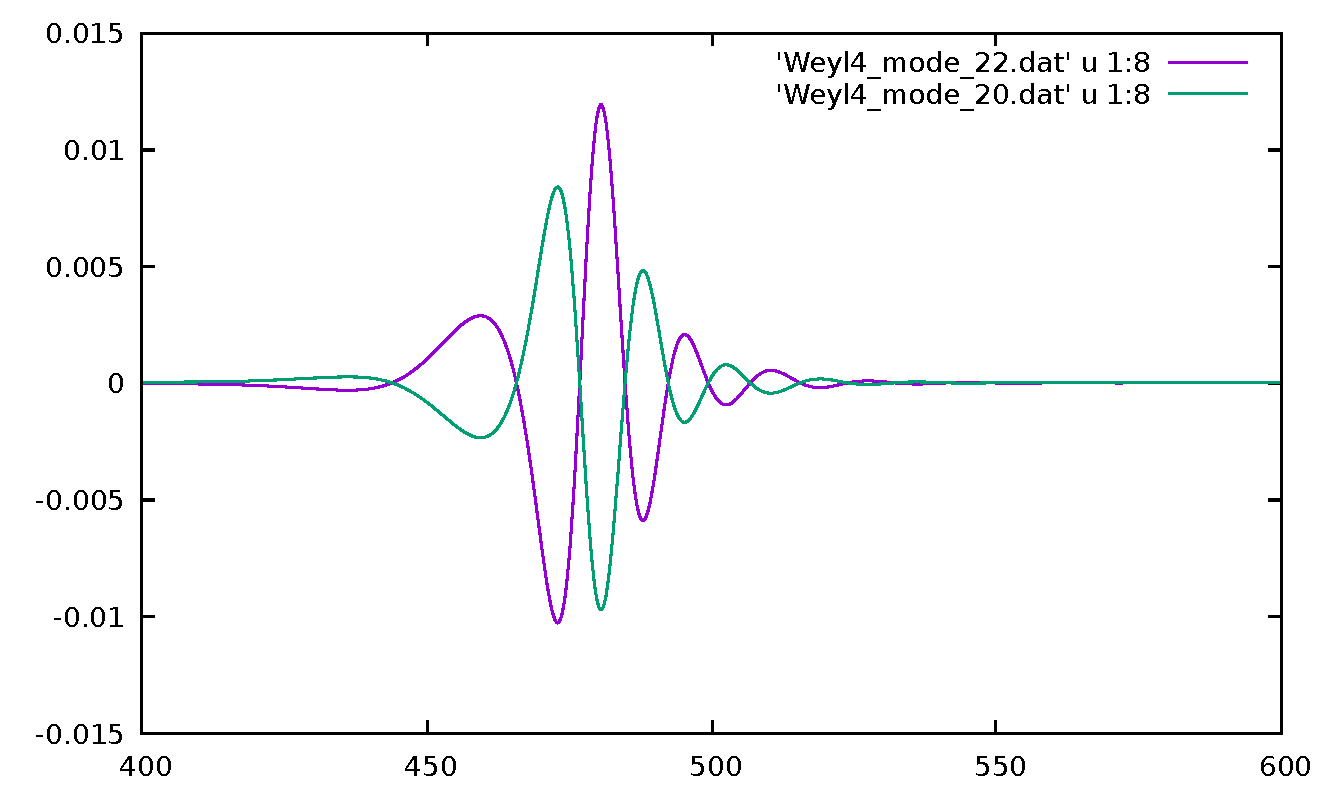
\includegraphics[width=0.5\textwidth]{data/headon_weyl22.pdf}\label{boson:fig:f14}}
% \end{figure}



% The dynamics of the two boson stars are shown in Fig.~(\ref{boson:fig:ff7}) plotting the scalar field modulus $|\vp|$ on the $x,y$ plane. The stars collide at at time $275\cdot m < t < 300 \cdot m$ and soon after an overdensity of scalar field forms collapsing to a black hole. This black hole subsequently accretes the surrouding scalar field; Fig.~(\ref{boson:fig:f7}) shows that the total Noether charge rapidly decays to zero as it falls into the black hole and is dissipated due to finite resolution effects. MAYBE DONT PUT THIS TWICE?

% as can be seen from the remnannt moving in (cvia coordinates) the simaultion is not in the rest frame.







%  \begin{figure}[h!]
%   \caption{Field plots of $|\vp|$ during evolution at four different times. Time $t=200 \cdot m$ and $t=250 \cdot m$ show snapshots momentarily before and after the collision. Time $t=300 \cdot m$ shows the scalar field accreting into the black hole and time $t= 400 \cdot m$ shows the scalar field surrounding the black hole a little later; noteably the amplitude is lower. All plots have a contour plot of $\chi=0.25$ acting as a very approximate marker for the event horizon. The Newtonian estimate of collision time is $t= 287.6 \cdot m$.}
%   \subfloat{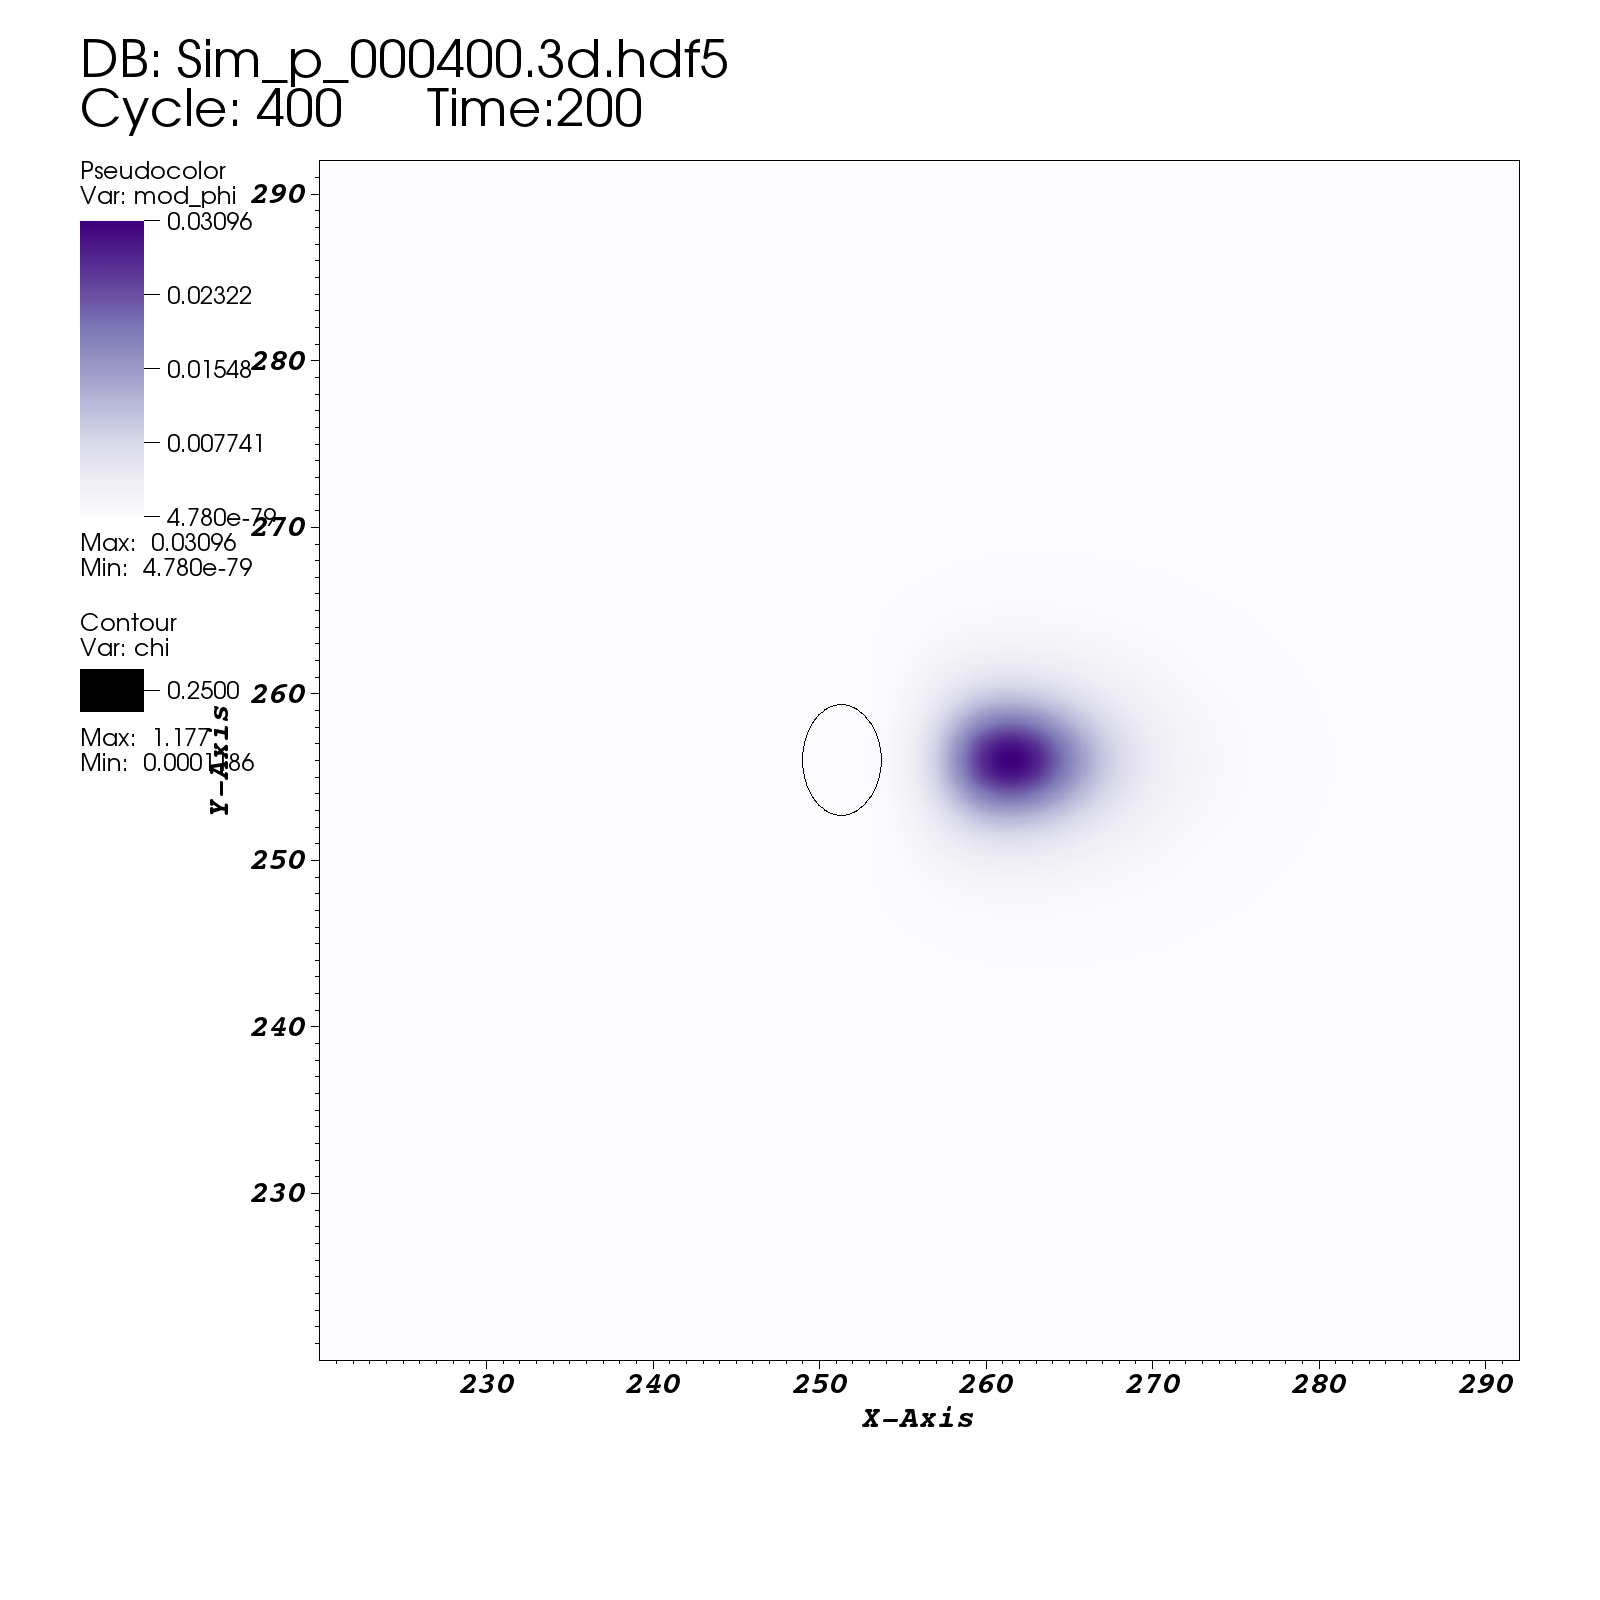
\includegraphics[width=0.45\textwidth]{modphi/headon_bhbs_mod_phi0008.png}\label{boson:fig:ff12}}
%   \subfloat{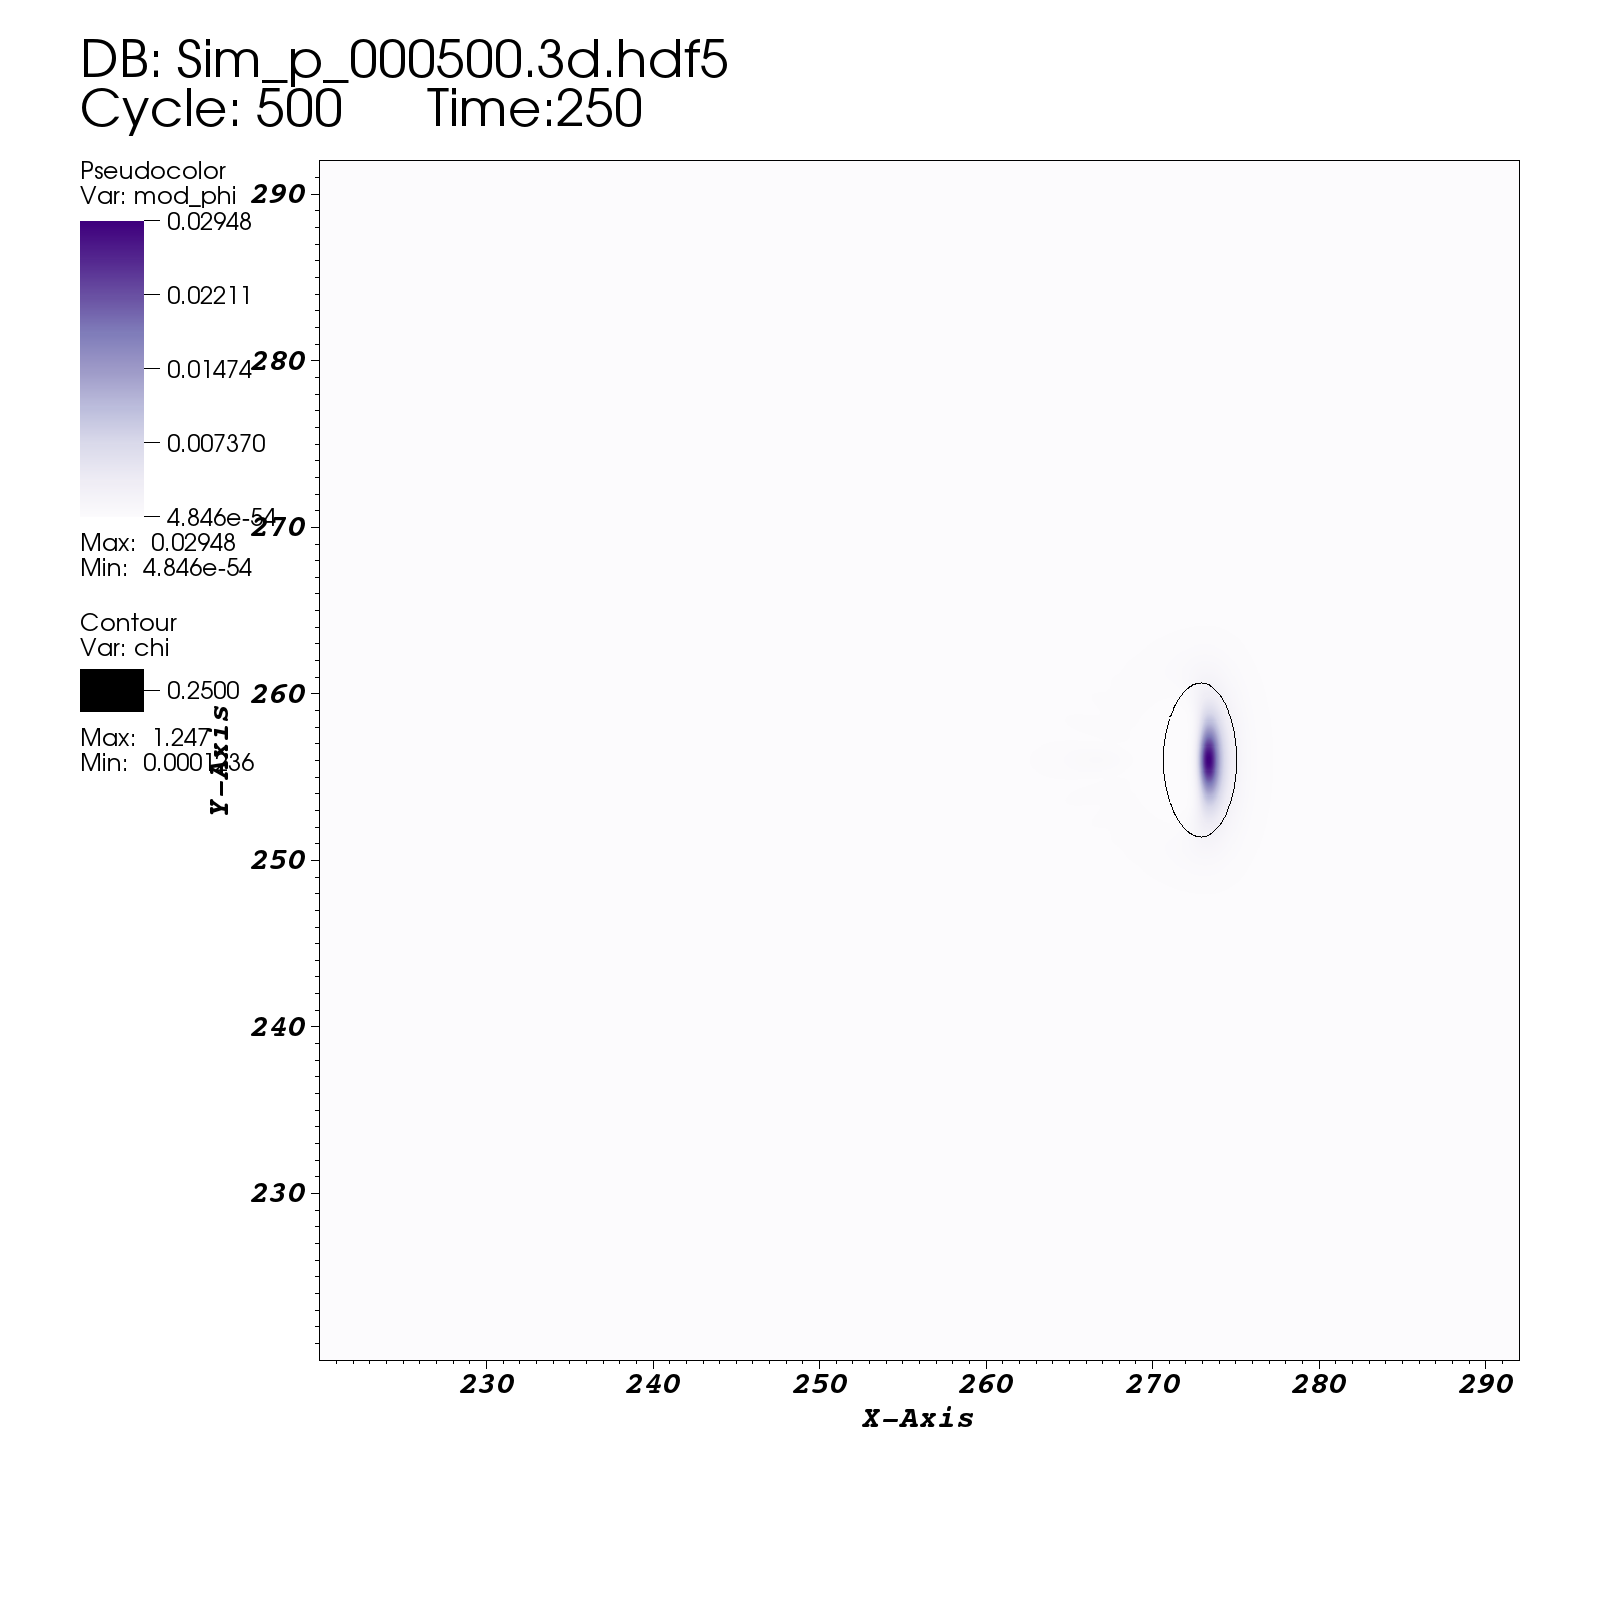
\includegraphics[width=0.45\textwidth]{modphi/headon_bhbs_mod_phi0010.png}}
%   \hfill
%   \subfloat{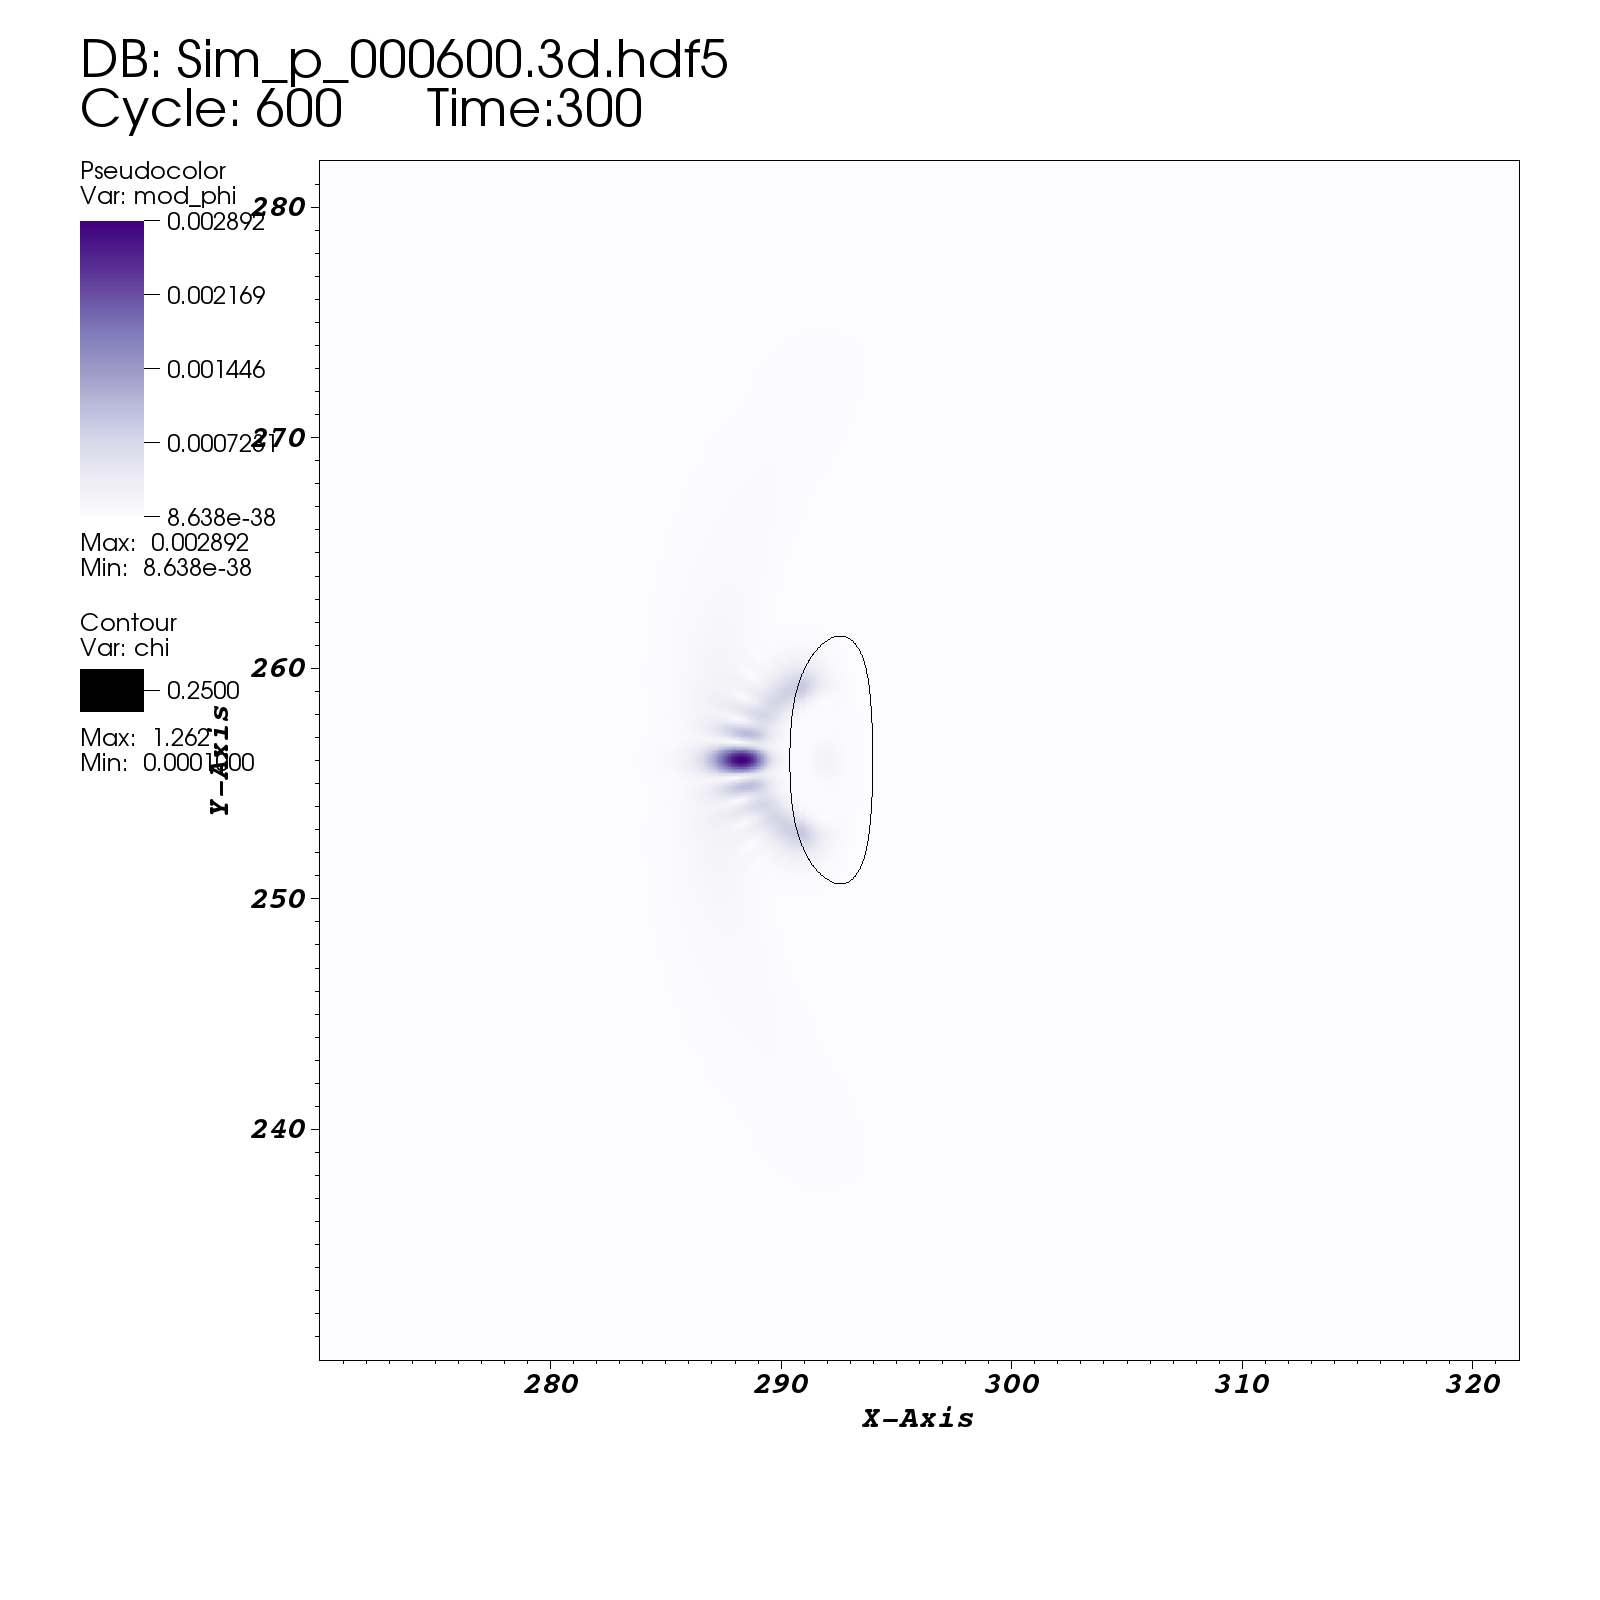
\includegraphics[width=0.45\textwidth]{modphi/headon_bhbs_mod_phi0012.png}}
%   \subfloat{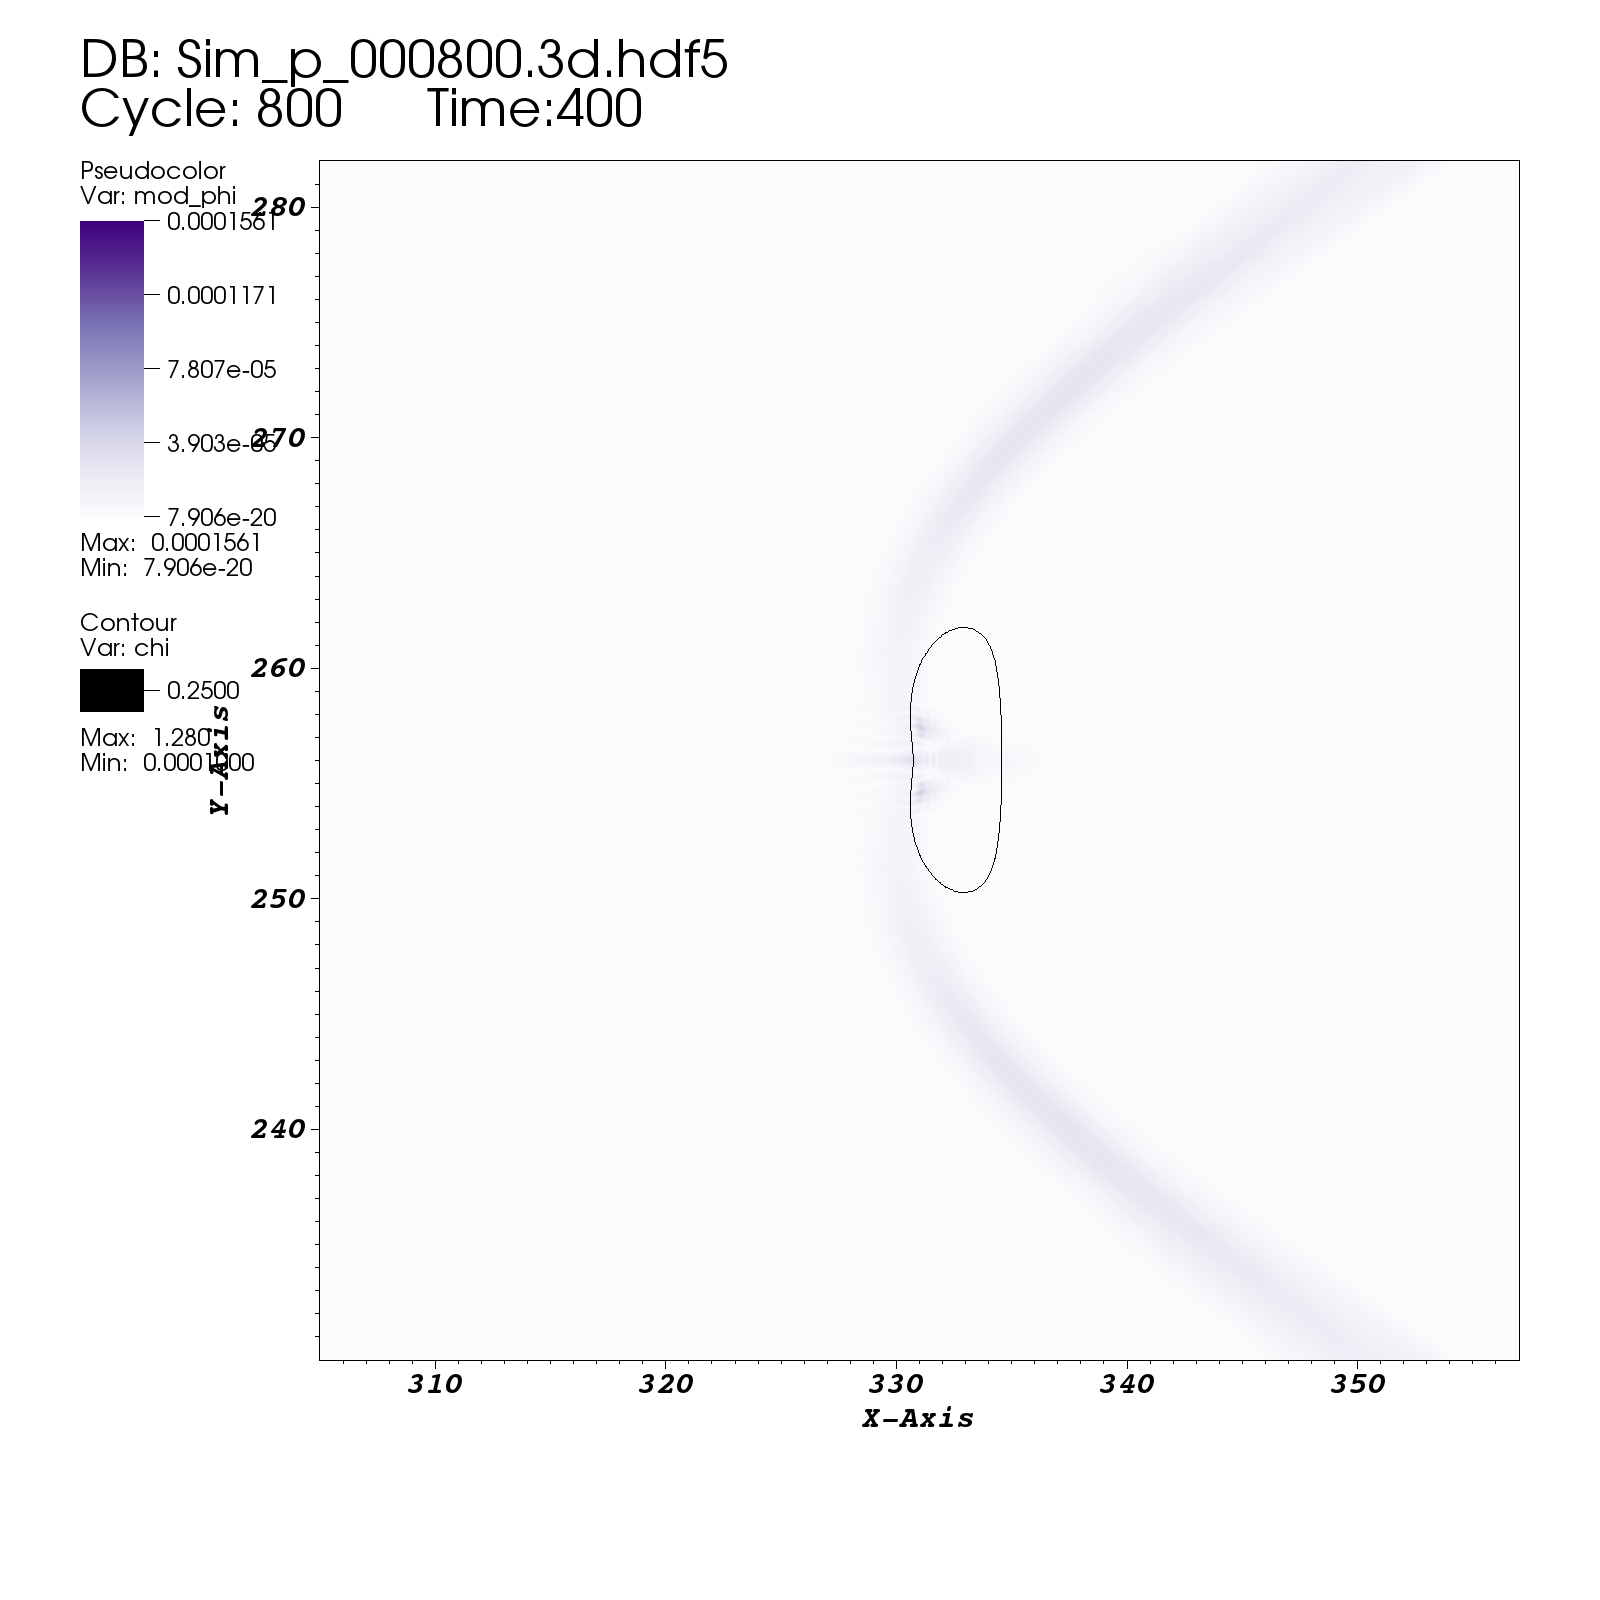
\includegraphics[width=0.45\textwidth]{modphi/headon_bhbs_mod_phi0016.png}}
% \end{figure}




% \subsubsection{Grazing Collision}
%  \begin{figure}[h!]
%   \caption{Left: Maximum of $|\vp|$ during evolution, Right: Total integrated Noether charge $N$.}
%   \centering
%   \subfloat{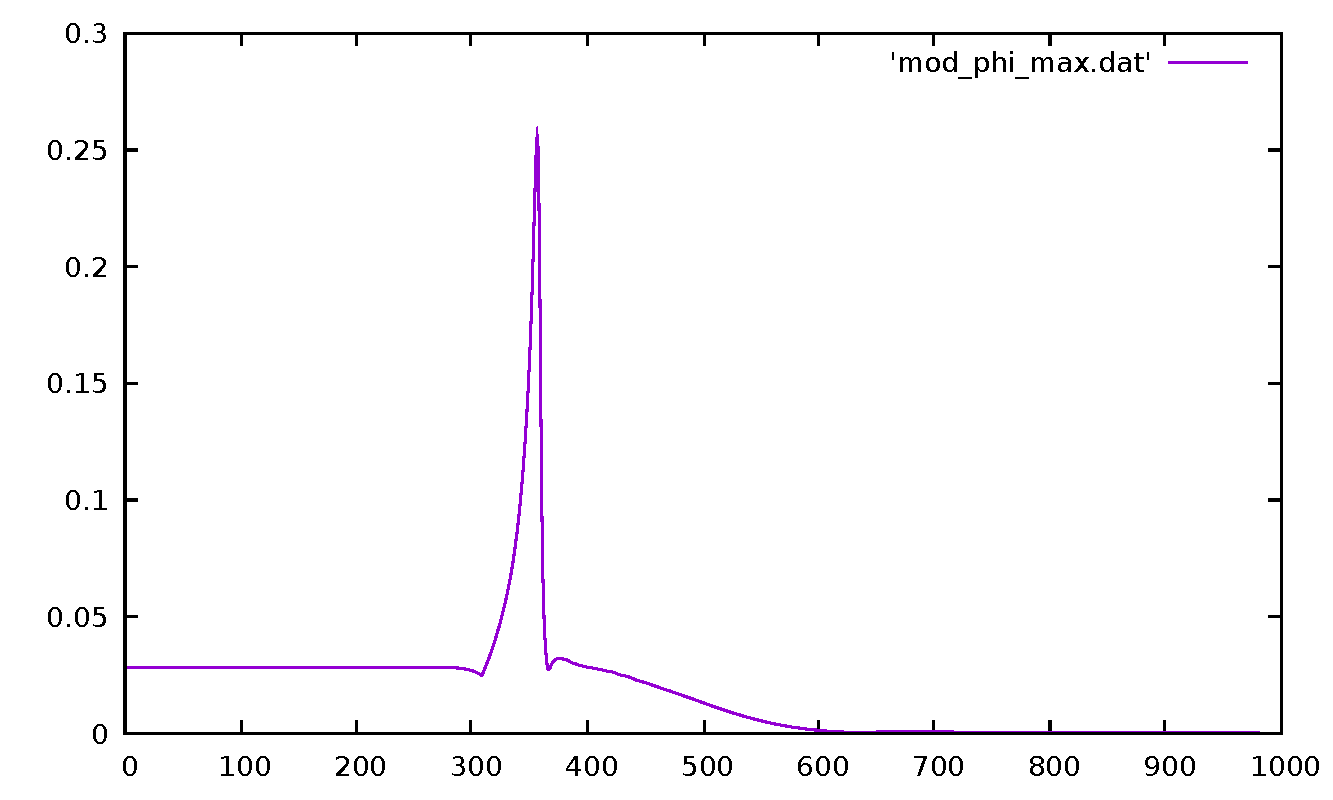
\includegraphics[width=0.5\textwidth]{data/graze_modphi.pdf}\label{boson:fig:f15}}
%   \hfill
%   \subfloat{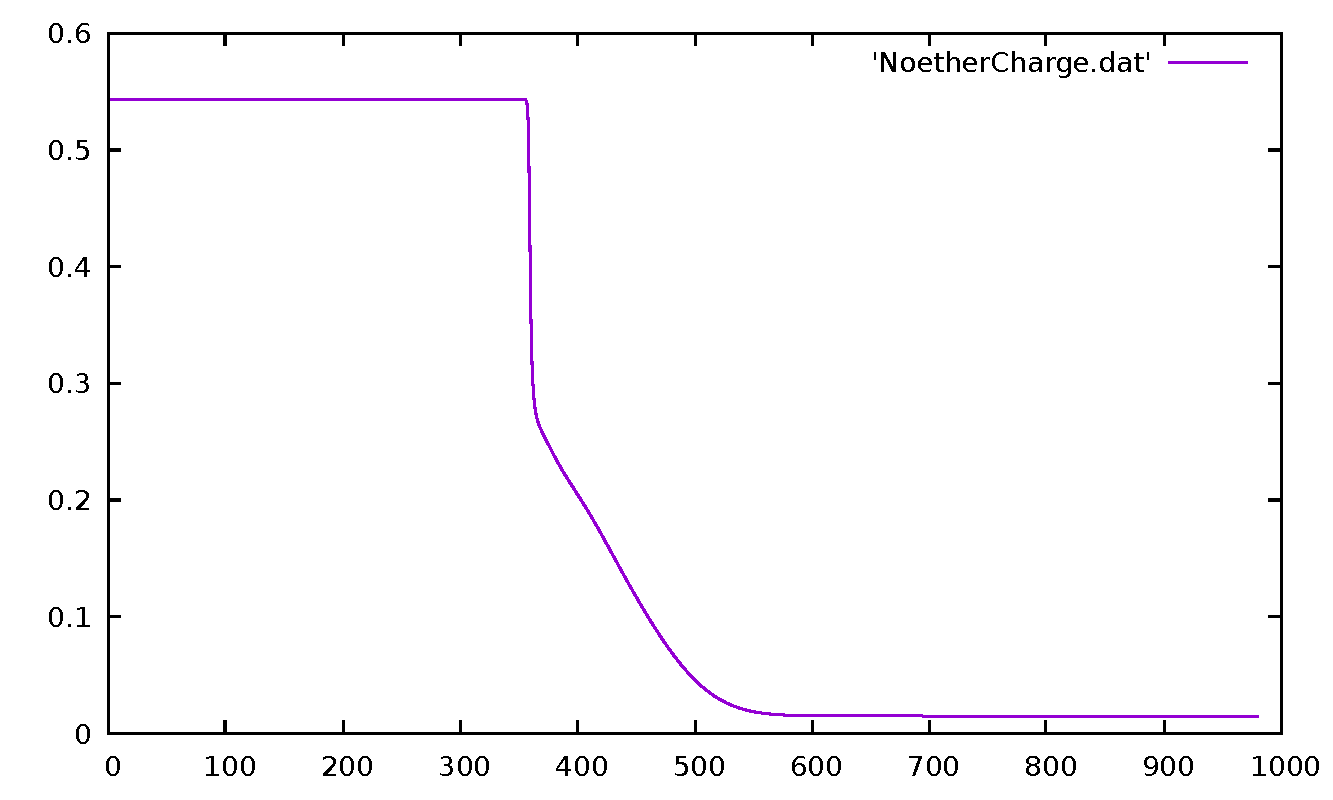
\includegraphics[width=0.5\textwidth]{data/graze_N.pdf}\label{boson:fig:f16}}
% \end{figure}

% Figure (\ref{boson:fig:f7}) shows $|\vp|_{\rm max}$, the global maximum value of $|\vp|$, and the total Noether charge as a function of time for the headon collision. At time $t\approx 289 \cdot m$, $|\vp|_{\rm max}$ rapidly increases; a black hole is then formed. At time $t\approx 327 \cdot m$, $|\vp|_{\rm max}$ there is a temporal maximum in $|\vp|_{\rm max}$ as the resolution limit of the simulation is reached and the scalar field is damped away by the Kreiss-Oliger dissipation mentioned in section \ref{grchombo:sec:grchombo}. This damping can also be seen in the Noether charge plot, at a time of $t \approx 326 \cdot m$, where the total charge that should remain constant falls. The lack of sufficient resolution inside the black hole is not disasterous to the external simulation fortunately; the erorrs accumulated are trapped inside the event horizon.

% The gravitational wave extraction at radius $r=140 \cdot m$ is given in figure \ref{boson:fig:f9}. A spin-weighted spherical harmonic decomposition of the Newman-Penrose scalar $\Psi_4$ [REF] has been done and the $m,l = 2,0$ and $m,l = 2,2$ modes are plotted.


% \begin{figure}[h!]
%   \caption{Left: Maximum of $|\vp|$ during evolution, Right: Total integrated Noether charge $N$.}
%   \centering
%   \subfloat{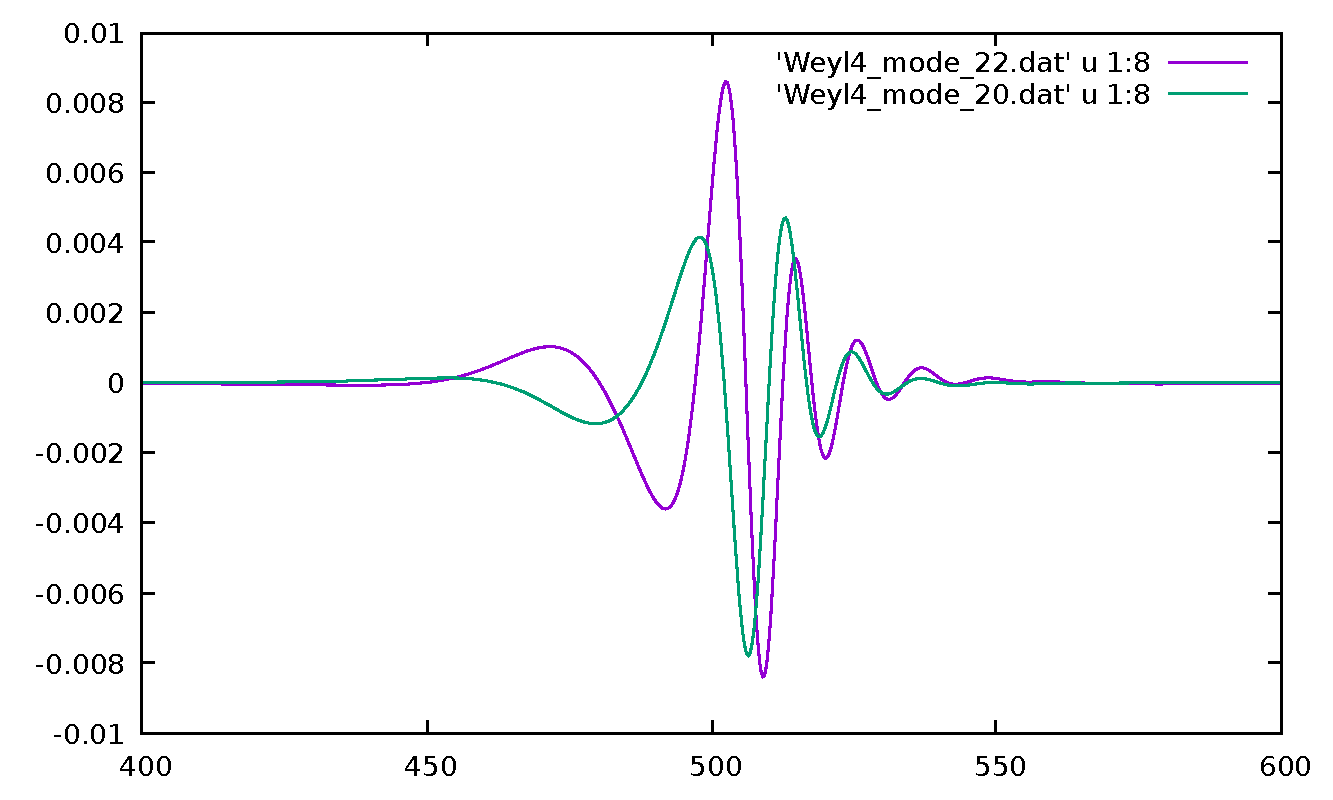
\includegraphics[width=0.5\textwidth]{data/graze_weyl22.pdf}\label{boson:fig:f17}}
% \end{figure}

% The dynamics of the two boson stars are shown in Fig.~(\ref{boson:fig:ff7}) plotting the scalar field modulus $|\vp|$ on the $x,y$ plane. The stars collide at at time $275\cdot m < t < 300 \cdot m$ and soon after an overdensity of scalar field forms collapsing to a black hole. This black hole subsequently accretes the surrouding scalar field; Fig.~(\ref{boson:fig:f7}) shows that the total Noether charge rapidly decays to zero as it falls into the black hole and is dissipated due to finite resolution effects. MAYBE DONT PUT THIS TWICE?



%  \begin{figure}[h!]
%   \caption{Left: Maximum of $|\vp|$ during evolution, Right: Total integrated Noether charge $N$.}
%   \subfloat{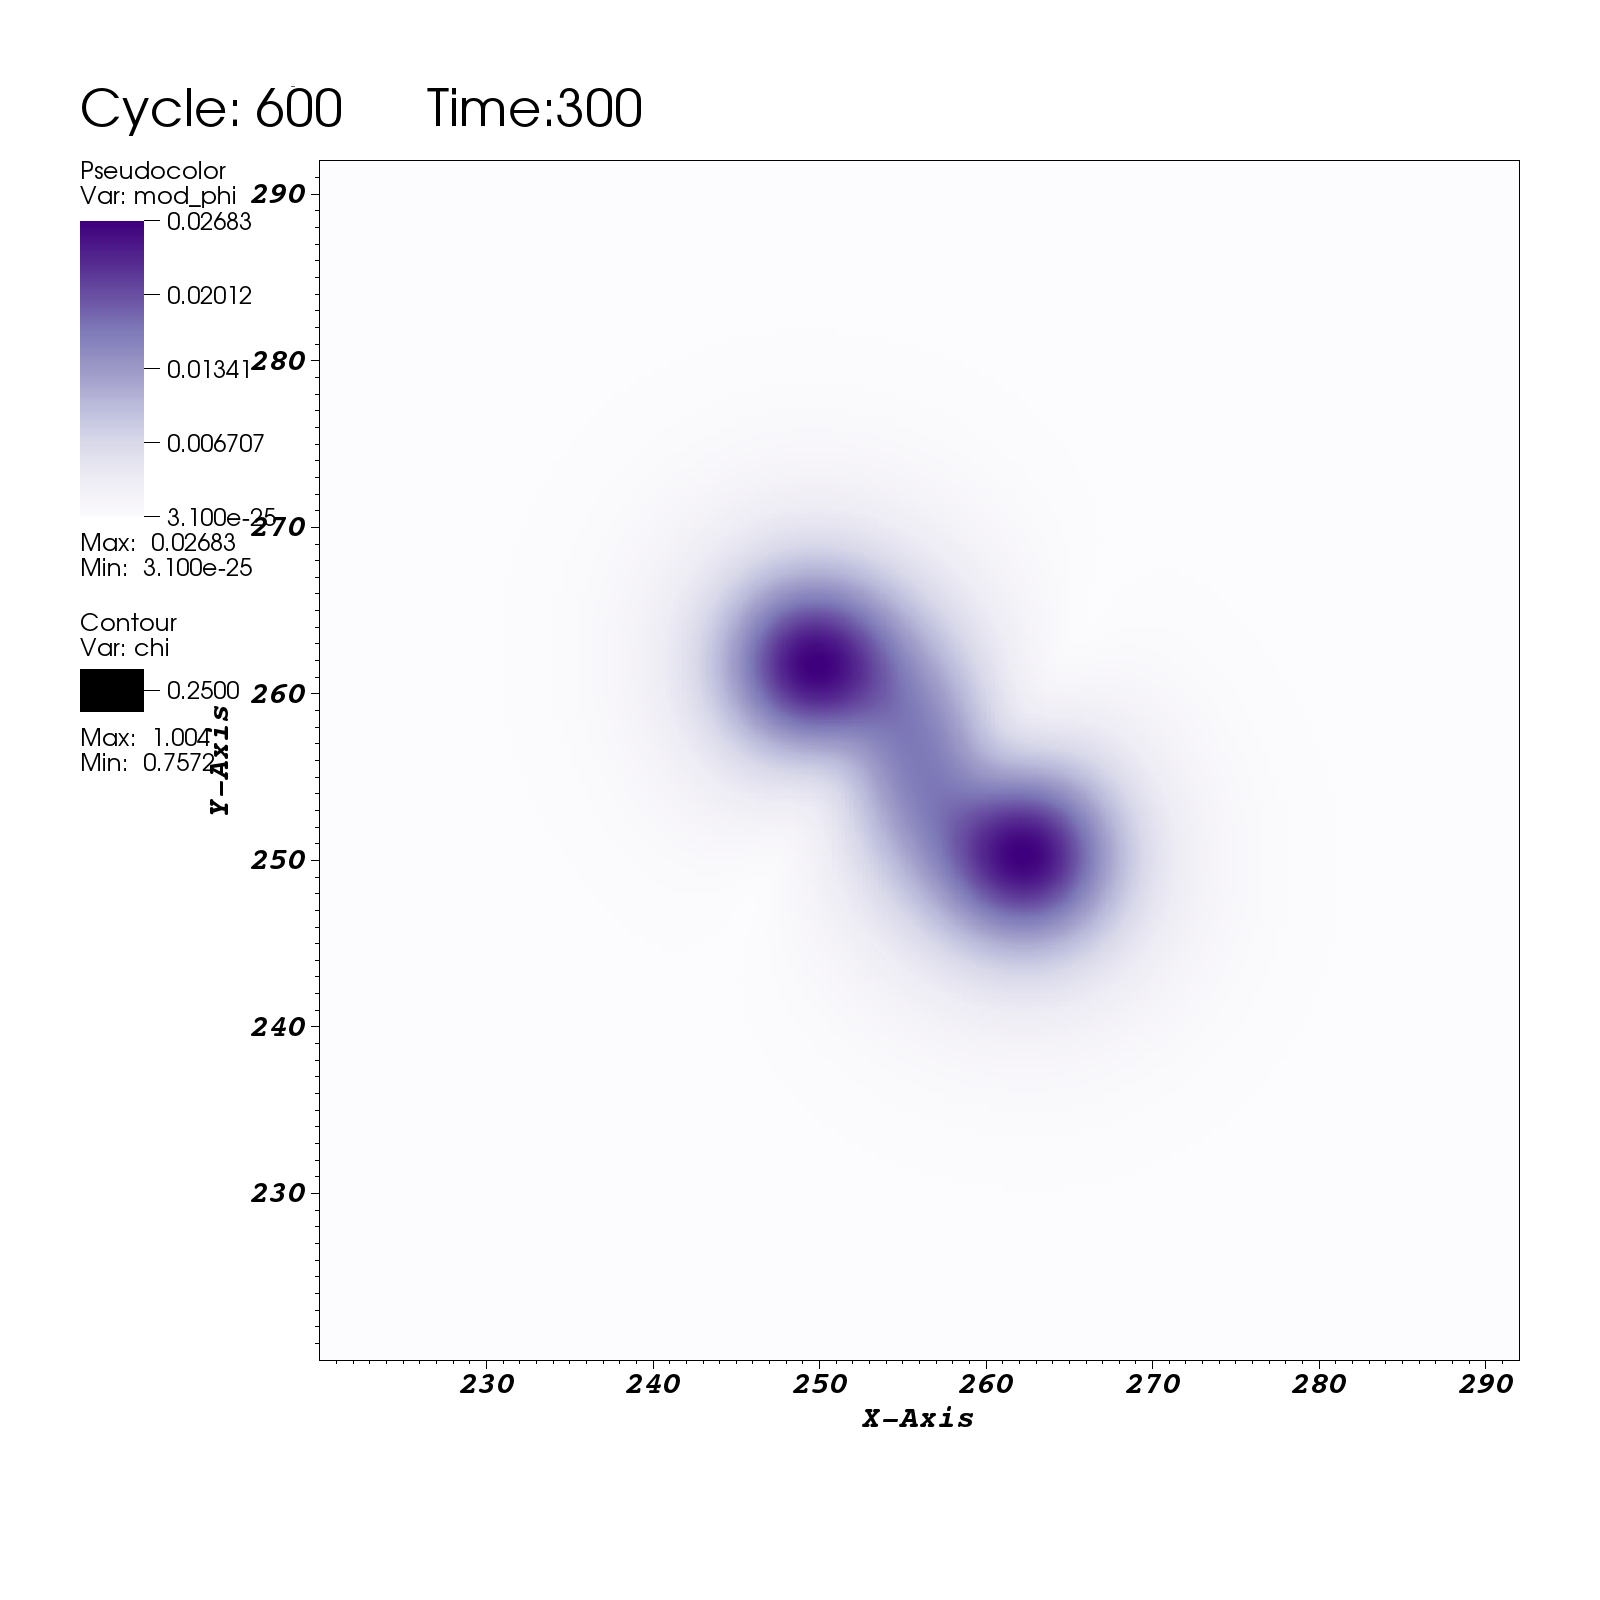
\includegraphics[width=0.45\textwidth]{modphi/graze_mod_phi0012.png}\label{boson:fig:ff15}}
%   \subfloat{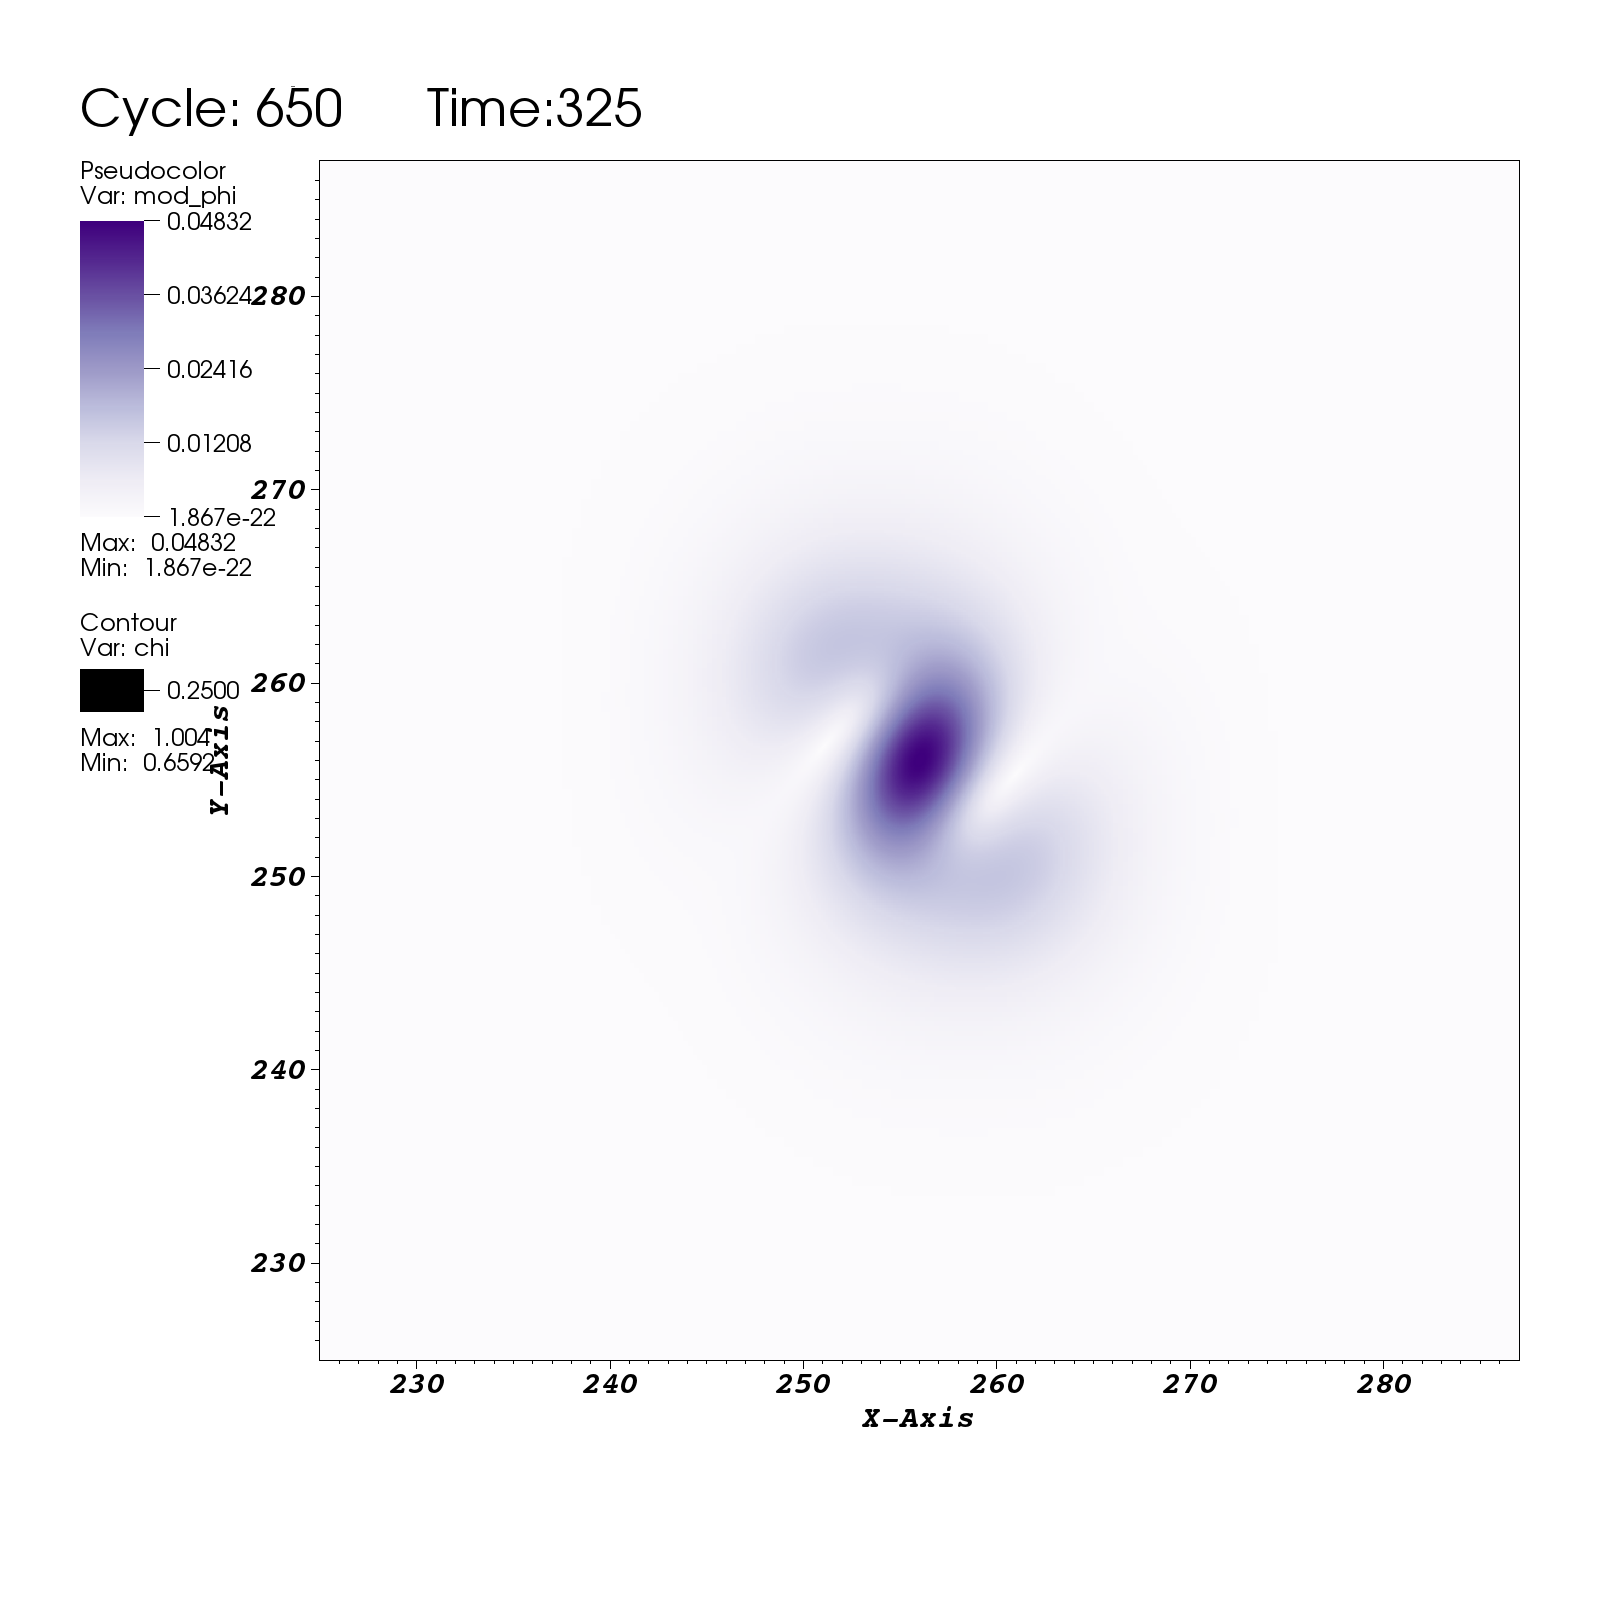
\includegraphics[width=0.45\textwidth]{modphi/graze_mod_phi0013.png}}
%   \hfill
%   \subfloat{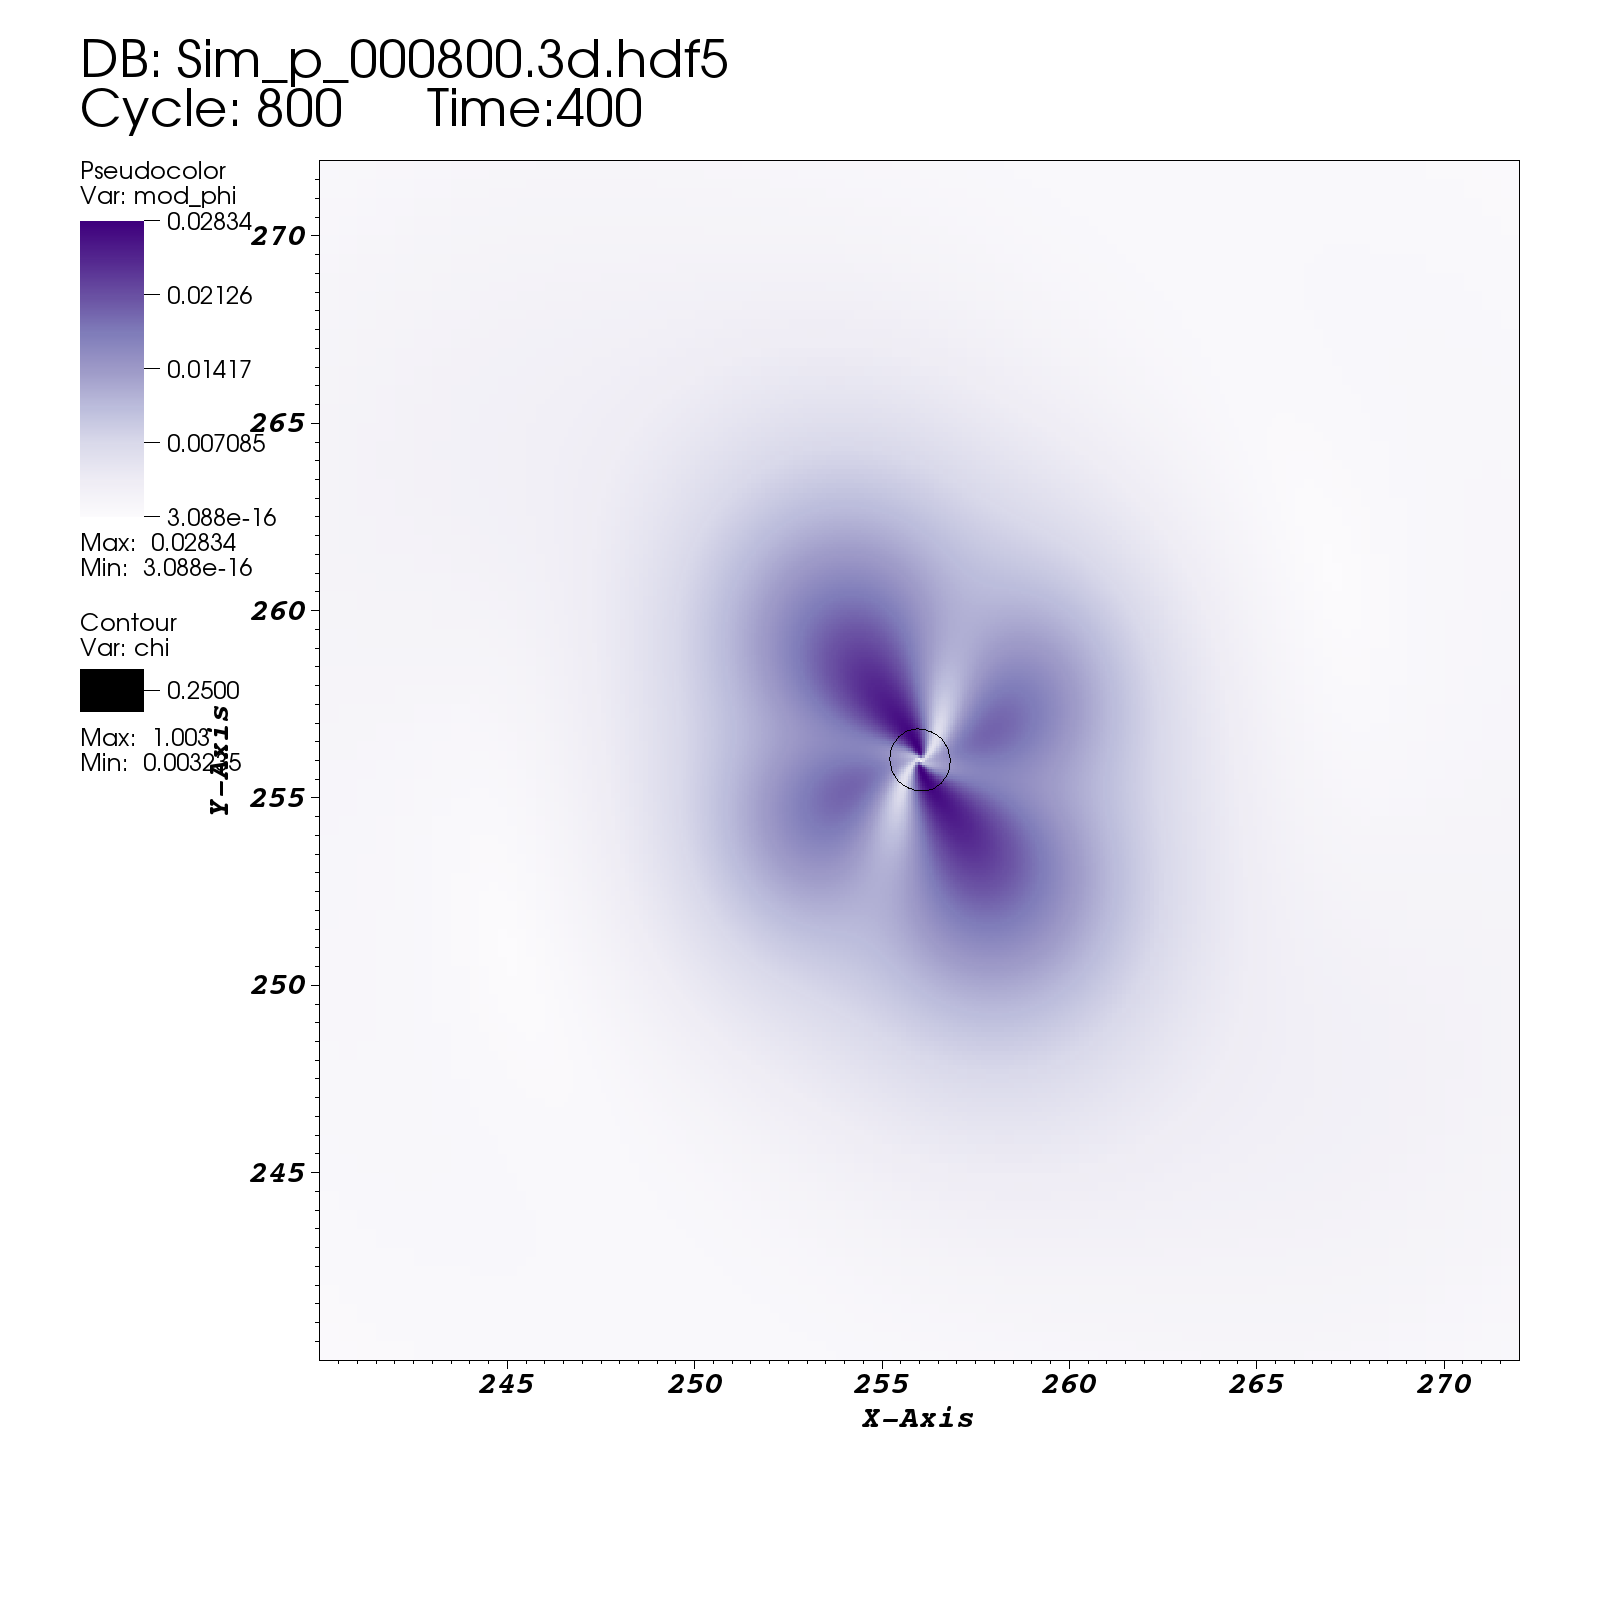
\includegraphics[width=0.45\textwidth]{modphi/graze_mod_phi0016.png}}
%   \subfloat{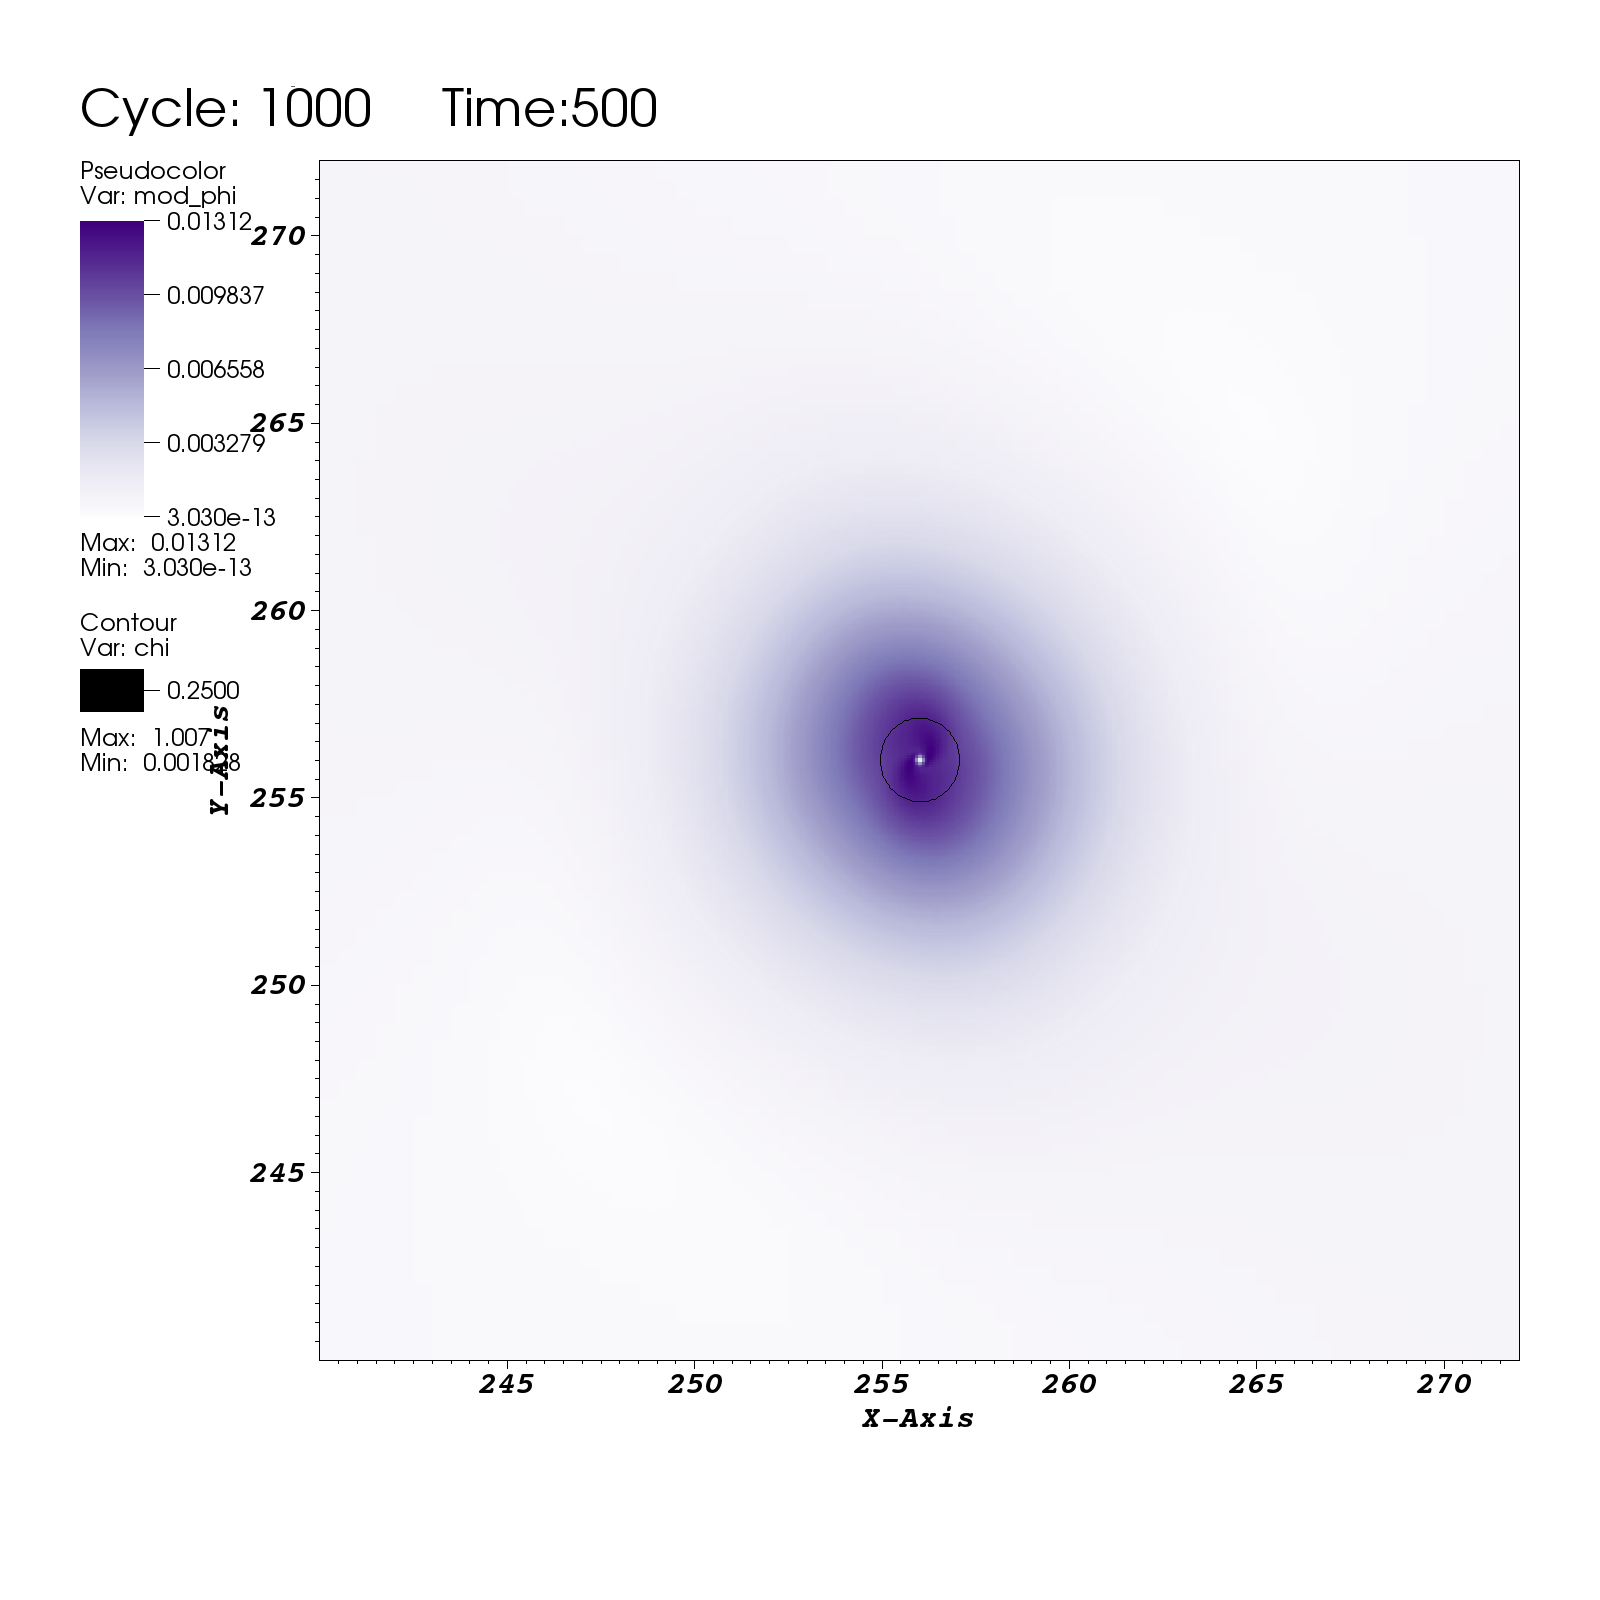
\includegraphics[width=0.45\textwidth]{modphi/graze_mod_phi0020.png}}
% \end{figure}








% THIS WAS ALWAYS UNCOMMENTED, STUFF ABOVE HERE MIGHT BE USEFUL
% THIS WAS ALWAYS UNCOMMENTED, STUFF ABOVE HERE MIGHT BE USEFUL
% THIS WAS ALWAYS UNCOMMENTED, STUFF ABOVE HERE MIGHT BE USEFUL
% THIS WAS ALWAYS UNCOMMENTED, STUFF ABOVE HERE MIGHT BE USEFUL
% THIS WAS ALWAYS UNCOMMENTED, STUFF ABOVE HERE MIGHT BE USEFUL
% THIS WAS ALWAYS UNCOMMENTED, STUFF ABOVE HERE MIGHT BE USEFUL
% THIS WAS ALWAYS UNCOMMENTED, STUFF ABOVE HERE MIGHT BE USEFUL
% THIS WAS ALWAYS UNCOMMENTED, STUFF ABOVE HERE MIGHT BE USEFUL
% THIS WAS ALWAYS UNCOMMENTED, STUFF ABOVE HERE MIGHT BE USEFUL
% THIS WAS ALWAYS UNCOMMENTED, STUFF ABOVE HERE MIGHT BE USEFUL
% THIS WAS ALWAYS UNCOMMENTED, STUFF ABOVE HERE MIGHT BE USEFUL










































% \newpage
% \newpage
% \newpage
% \newpage
% \newpage
% \newpage
% \newpage

% \subsection{After Here is Basically Junk}

% \subsection{Head-on Collisions}
% All the cases studied here are for stationary initial data $\tilde{\A}_{ij}=0,\K=0$ in-falling from an initial separation of $d \cdot m = 32$ due to gravitational attraction. Firstly we consider the equal mass Boson star binary, initial data in figure (). At first they slowly infall creating a short lived object with three maxima, shown in figure (,left), then collapse to a black hole with a decaying spherical harmonic cloud (figures ) outside. As with all the simulations from now on we assume a black hole forms if $\chi \ll 16^{-1}$ where $\chi=16^-1$ is the value taken on the horizon for the isotropic Schwarzschild metric.
%   \begin{figure}[h!]
%   \caption{Initial Data, Left: $\chi$, Right: $|\vp|$.}
%   \centering
%   \subfloat{\includegraphics[width=0.5\textwidth]{headon_bs/chi0000.png}\label{boson:fig:f9}}
%   \hfill
%   \subfloat{\includegraphics[width=0.5\textwidth]{headon_bs/modphi0000.png}\label{boson:fig:f10}}
% \end{figure}
%   \begin{figure}[h!]
%   \caption{Scalar field amplitude before and after black hole formation, Left: Time $t\cdot m = 150$, Right: Time $t \cdot m = 200$.}
%   \centering
%   \subfloat{\includegraphics[width=0.5\textwidth]{headon_bs/modphi0003.png}\label{boson:fig:f11}}
%   \hfill
%   \subfloat{\includegraphics[width=0.5\textwidth]{headon_bs/modphi0004.png}\label{boson:fig:f12}}
% \end{figure}
%    \begin{figure}[h!]
%   \caption{Real part of scalar field after black hole formation, Left: xy plane, Right: yz plane, perpendicular to initial star separation.}
%   \centering
%   \subfloat{\includegraphics[width=0.5\textwidth]{headon_bs/phi_re0004.png}\label{boson:fig:f13}}
%   \hfill
%   \subfloat{\includegraphics[width=0.5\textwidth]{headon_bs/phi_re_perp0004.png}\label{boson:fig:f14}}
% \end{figure}

% The second case considered is the same Boson star outside a black hole parameterised by $M=10M_{BS}$ where $M_{BS}$ is the ADM mass of the Boson star. The scalar field tidally deforms into an ellipsoid with high central density, well beyond Kaup limit of $\vp(0)\sim 0.0764$, and spontaneous collapse to a smaller external black hole is observed. After collapse, figure (), there is an elongated cloud about the new small black hole; there are many nodal lines in $\mathrm{Re}(\vp)$ which focus on the large black hole showing the cloud is in-falling.

%   \begin{figure}[h!]
%   \caption{Initial Data, Left: $\chi$, Right: $|\vp|$.}
%   \centering
%   \subfloat{\includegraphics[width=0.5\textwidth]{LMR/chi0000.png}\label{boson:fig:f15}}
%   \hfill
%   \subfloat{\includegraphics[width=0.5\textwidth]{LMR/modphi0000.png}\label{boson:fig:f16}}
% \end{figure}
%   \begin{figure}[h!]
%   \caption{Final Data at time $t\cdot m = 125$, Left: Conformal factor $\chi$, Right: Scalar field modulus $|\vp|$, Bottom: Real part of scalarfield $\mathrm{Re}(\vp).$}
%   \centering
%   \subfloat{\includegraphics[width=0.5\textwidth]{LMR/chi0005.png}\label{boson:fig:f17}}
%   \hfill
%   \subfloat{\includegraphics[width=0.5\textwidth]{LMR/modphi0005.png}\label{boson:fig:f18}}
%   \\
%    \subfloat{\includegraphics[width=0.5\textwidth]{LMR/phi_re0000.png}\label{boson:fig:f19}}
% \end{figure}
% Final case consists of an equal mass Black Hole and Boson Star, initial configuration in Figure 11. As can be seen from the plot of $\Re(\phi)$ and $|\phi|$, in Figure 12, most of the star falls into the black hole, however some scalar field manages to excite an intricate spherical harmonic cloud pattern.
%   \begin{figure}[h!]
%   \caption{Initial data for equal mass Boson Star and Black Hole, Left: $\chi$, Right: $|\vp|$}
%   \centering
%   \subfloat{\includegraphics[width=0.5\textwidth]{headon/chi0000.png}\label{boson:fig:f20}}
%   \hfill
%   \subfloat{\includegraphics[width=0.5\textwidth]{headon/mod_phi0000.png}\label{boson:fig:f21}}
% \end{figure}
%   \begin{figure}[h!]
%   \caption{Time $t\cdot m=905$ for equal mass Boson Star and Black Hole, Left: $\Re(\vp)$, Right: $|\vp|$}
%   \centering
%   \subfloat{\includegraphics[width=0.5\textwidth]{headon/phi_re0000.png}\label{boson:fig:f22}}
%   \hfill
%   \subfloat{\includegraphics[width=0.5\textwidth]{headon/mod_phi0007.png}\label{boson:fig:f23}}
% \end{figure}

% In all three cases, the Noether charge drops rapidly upon the formation of a black hole; this will be explained in the next section. However some scalar field lingers after collapse, in each case the hair takes the form of spherical harmonics discussed in (). Also observed is the decay of the spherical harmonics to zero amplitude in these simulations with no angular momentum.

% \subsection{Binary Inspiral}
% The only considered case here is the Quasi-circular orbit and inspiral of two equal mass boson stars. The initial boosts were determined by a newtonian calculation yielding
% \begin{equation} v^2 = \frac{M}{2d}\end{equation}
% where $M=0.53(29)$ is the ADM mass of the Boson Star and d is the initial separation. For a relatively low separation of $d\cdot m =32$ code units, shown in Figures 13,14 (Left), we get $v \sim 0.0915$. The boson stars are observed to complete roughly half an orbit before merging and collapse, forming a black hole. Here a Kerr black hole is assumed to have formed as the spacetime has a significant angular momentum which should partially infall with the scalar field.

%   \begin{figure}[h!]
%   \caption{Boson Star $|\vp|$. Left: initial data, Right: later time $t \cdot m = 700$}
%   \centering
%   \subfloat{\includegraphics[width=0.5\textwidth]{inspiral/mod_phi_inspiral_nice0000.png}\label{boson:fig:f24}}
%   \hfill
%   \subfloat{\includegraphics[width=0.5\textwidth]{inspiral/mod_phi_inspiral_nice0002.png}\label{boson:fig:f25}}
% \end{figure}
%   \begin{figure}[h!]
%   \caption{Boson Star $\Re(\vp)$. Left: initial data, Right: later time $t \cdot m = 700$}
%   \centering
%   \subfloat{\includegraphics[width=0.5\textwidth]{inspiral/phi_inspiral_nice0000.png}\label{boson:fig:f26}}
%   \hfill
%   \subfloat{\includegraphics[width=0.5\textwidth]{inspiral/phi_inspiral_nice0002.png}\label{boson:fig:f27}}
% \end{figure}
%   \begin{figure}[h!]
%   \caption{Left: Total Noether charge $\mathcal{N}$ during evolution, Right: $\Psi_4$ over 22 harmonic during evolution.}
%   \centering
%   \subfloat{\includegraphics[width=0.5\textwidth]{inspiral/N.png}\label{boson:fig:f28}}
%   \hfill
%   \subfloat{\includegraphics[width=0.5\textwidth]{inspiral/GW.png}\label{boson:fig:f29}}
% \end{figure}
% Figure 15 shows the total Noether charge, which is no longer conserved. When the black hole forms, the in-falling scalar field moves towards zero radius and gets hugely compressed. The huge compression causes extreme field gradients which induces continuous regridding in the AMR, but this is capped at 7 layers in this simulation to make runtime feasible. When the 8th AMR level is needed it is simply not added and resolution becomes low enough that any Noether charge near the centre is so under-resolved that it seems to fall between the gridpoints. Interestingly, Figures 13,14 (Right) show a scalar field configuration lingering around the black hole, mostly outside the contour $\chi=0.7$, looking like scalar hair. Also Figure 15 (Left) of the Noether charge appears to take significantly longer to decay than in the linear collision simulations. It can be seen in Figure 14 in the plot of $\Re(\vp)$ that the cloud has angular nodes corresponding to angular momentum similarly to boosted stars picking up nodal planes perpendicular to momentum and Figure 10 (Bottom) of the infalling cloud.

% The gravitational wave (GW) signal can be seen in Figure 15 (Right), extracted at a radius $r \cdot m = 90$. At the time $t \cdot m \approx 700$ the gravitational wave signal due to the merger appears; in order to record a longer inspiral simulations with larger initial separations need to be simulated. Currently there appears to be some small problem with the initial data, also observed in the collisions with no angular momentum, that manifests itself in noisy GW extraction and the Hamiltonian constraint initially sharply rising.






%\newpage
%\pagenumbering{arabic}




\section{Mathematical Modelling of Boson Stars}
\subsection{The Action} \label{boson:sec:action}
The Boson Stars considered are a complex Klein Gordon Scalar field, $\varphi$, minimally coupled to gravity. The action is the Einstein-Hilbert vacuum action plus the matter action for curved space,
\begin{gather} S = \int_\mathcal{M}\left[\mathcal{L}_{EH} + \mathcal{L}_M\right] \sqrt{-g}\,\dd x^4, \\
 \L_{EH} = \frac{c^4}{16\pi G}R, \\
 \L_{M} =-\frac{1}{2}g^{\mu\nu}\nabla_\mu \bar{\varphi} \nabla_\nu \varphi - \frac{1}{2}V(|\varphi|^2),  \end{gather}
Here $V$ is the Klein-Gordon potential and it's effect on boson stars is discussed in \cite{Schunck:2003kk} \cite{Liebling:2012fv}. Some common choices of potentials are,
\begin{align}
V_{\rm mini} &= \frac{m^2 c^2}{\hbar^2 }|\vp|^2,\label{boson:eq:Vmini} \\
V_{\rm int} &= \frac{m^2 c^2}{\hbar^2 }|\vp|^2 + \frac{1}{2}\Lambda_4|\vp|^4 ,\\
V_{\rm soli} &= \frac{m^2 c^2}{\hbar^2 }|\vp|^2\left(1-\frac{|\vp|^2}{2\sigma^2}\right)^2 , \label{boson:eq:Vsoliton}
\end{align}
where $\hbar$ and $c$ are given for completeness but will be set to unity later.
Considering only the $m^2$ term, which corresponds to the squared mass of the particle in the quantum theory, we get a massive wave equation linear in $\varphi$, leading to so called {\it mini} Boson stars. Having $\Lambda_4\neq0$ gives {\it self-interacting} stars which have a nonlinear wave equation corresponding to particle creation and annihilation at the quantum level; self interacting potentials can include higher order terms in $\vp$ such as $|\vp|^6$, $|\vp|^8$ and more. These self interacting potentials tend to have star solutions with a higher density. Finally, Eq.~(\ref{boson:eq:Vsoliton}) describes the {\it solitonic} potential, giving rise to boson stars with compactness comparable to neutron stars. Solitonic boson stars and their gravitational
wave signatures have been studied in \cite{Palenzuela:2017kcg}.

Varying the action with respect to the metric and scalar field return the Einstein field equation and the Klein Gordon equation of curved space respectively,
\begin{align} R_{\mu\nu} - \frac{1}{2}R g_{\mu\nu} &=  \frac{8\pi G}{c^4} T_{\mu\nu}  ,\\
g^{\mu\nu}\nabla_\mu\nabla_\nu \vp &= \frac{\partial V}{\partial |\vp|^2}\vp .\label{boson:eq:KGeqn}\end{align}
Collectively these are known as the Einstein-Klein-Gordon (EKG) equations. From Eq.~(\ref{intro:eq:Tdef}), the boson-specific stress energy tensors are,
\begin{align}  
T_{\mu\nu} :&= -2\frac{\delta \mathcal{L}_{M}}{\delta g^{\mu\nu}}+g_{\mu\nu}\mathcal{L}_M, \\
T_{\mu\nu} &= \frac{1}{2}\nabla_{\mu}\bar{\varphi}\nabla_{\nu}\varphi+\frac{1}{2}\nabla_{\nu}\bar{\varphi}\nabla_{\mu}\varphi-\frac{1}{2}g_{\mu\nu}\left[g^{\alpha\beta}\nabla_\alpha\bar{\varphi}\nabla_\beta\varphi + V\right] \label{boson:eq:KGT}.
\end{align}
\subsubsection{Comparison of Boson Stars to Neutron Stars}
Boson stars differ greatly to neutron stars; studying neutron stars requires the fermionic, or ordinary fluid, stress tensor $\bs{T}_F$; 
\begin{equation} T^{\mu\nu}_F = \left[\rho c^2+ {P} \right]\frac{u^\mu u^\nu}{c^2} + P g^{\mu\nu} + 2u^{(\mu}q^{\nu)}+\pi^{\mu\nu}+ ...\,\,.\end{equation} 
The continuity equation from Eq.~(\ref{intro:eq:cont}), $\nabla_\nu T^{\mu\nu}=0 $, returns the highly nonlinear relativistic Navier-Stokes equations of curved space. The viscosity term $\pi^{\mu\nu}$ and heat flux $q^\mu$ are often omitted for simplicity. The remaining variables $\rho$, $P$ and $u^\mu$ are the fluid density, pressure and worldline tangent. Just as in flat space, the Navier-Stokes equations can develop shockwaves and the use of sophisticated shock capturing schemes is required, unlike the linear Klein-Gordon equation which is linear in the principal part.


\subsection{Solitons} \label{boson:sec:soliton}
A soliton is a wave packet that exhibits particle-like behaviour. More precisely, in classical field theory, a soliton
is a field or set of fields in a localised configuration that travels at constant speed without dispersing. This is a property of solutions to the linear wave equation but many solitonic solutions exist for non-linear differential equations as well. For
our purposes, we look for solitons in the Einstein-Klein-Gordon (EKG) system which are self gravitating
localised scalar field and metric configurations. In the case of the real scalar field it was shown that
there are no long lived solitons \cite{diez2013no}; however promoting the field to a complex scalar we can find a spherically
symmetric stationary soliton with the following configuration,
\begin{equation} \varphi = \Phi(r)e^{i\omega t}, \label{boson:eq:fieldansatz} \end{equation}
in spherical polar coordinates $x^\mu \in \{t,r,\theta,\phi \}$.
Traditionally, the polar areal gauge has been used for the metric's ansatz,
\begin{equation}g_{\mu\nu}\dd x^\mu \dd x^\nu =- a^2(r)\dd t^2 + b^2(r) \dd r^2 + r^2 \left[ \dd \theta^2 + \sin^2\theta \dd \phi^2\right],\label{boson:eq:polaransatz}\end{equation}
where the boundary condition $b^2(0)=1$ is demanded to avoid a conical singularity at the origin. However an isotropic gauge is more useful for simulations due to easier conversion to Cartesian space-coordinates, for more information on isotropic coordinates see section \ref{intro:sec:bh_theory}. The polar areal solution must then be transformed into an isotropic solution. Alternatively, the approach taken in this report, is to start with an isotropic ansatz,
\begin{equation} g_{\mu\nu}\dd x^\mu \dd x^\nu =- \Omega^2(r)\dd t^2 + \Psi^2(r)\dd \bm{x}^2,\label{boson:eq:metricansatz}\end{equation}
where $\dd \bm{x}^2$ denotes the euclidean 3D line element; this changes between spherical polar or Cartesian coordinates trivially. This ends up being slightly harder to solve for numerically, but no conversion to isotropic coordinates is needed afterwards.

To get a set of ODEs to solve for the functions $\{\Omega(r), \Psi(r),\Phi(r)\}$ we must turn to the Einstein equation and Klein Gordon equation. The Einstein equations for $\{\mu,\nu\}=\{0,0\},\{1,1\},\{2,2\}$ are the only components that give unique non-zero equations in spherical symmetry; they are,
\begin{gather}
\frac{\Omega ^2 \left[r \Psi '^2-2 \Psi  \left[r \Psi ''+2 \Psi '\right]\right]}{r \Psi ^4} = 4\pi G \left[\Omega ^2 \left[\frac{\Phi'^2}{\Psi ^2}+V\right]+\omega ^2 \Phi^2\right],\\
\frac{2 \Psi  \Psi ' \left[r \Omega '+\Omega \right]+r \Omega  \Psi '^2+2 \Psi ^2 \Omega
   '}{r \Psi ^2 \Omega } = 4\pi G \left[\Phi'^2-\Psi ^2 V+\frac{\omega ^2 \Phi^2 \Psi ^2}{\Omega
   ^2}\right],\\
   r \left[-\frac{r \Psi '^2}{\Psi ^2}+\frac{r \Psi ''+\Psi '}{\Psi }+\frac{r \Omega ''+\Omega
   '}{\Omega }\right] = -4\pi G r^2 \Psi ^2 \left[\frac{\Phi'^2}{\Psi ^2}+V-\frac{\omega ^2 \Phi^2}{\Omega
   ^2}\right],
   \end{gather}
  where the Einstein tensor $G_{\mu\nu} = R_{\mu\nu}-\frac{1}{2}R g_{\mu\nu}$  and the stress tensor $T_{\mu\nu}$ are on the left and right respectively. Substituting the metric ansatz Eq.~(\ref{boson:eq:metricansatz}) and the field ansatz Eq.~(\ref{boson:eq:fieldansatz}) into Eq.~(\ref{boson:eq:KGeqn}), the Klein Gordon equation becomes,
  \begin{align}
  g^{\mu\nu}\nabla_\mu\nabla_\nu \vp &= \frac{\partial V}{\partial |\vp|^2}\vp ,\\
   \frac{1}{\sqrt{-g}}\partial_\mu \left[ \sqrt{-g}g^{\mu\nu}\partial_\nu \Phi(r)e^{i\omega t}\right] &= \frac{\partial V}{\partial |\vp|^2} \Phi(r)e^{i\omega t} ,\\
  \Phi'' = \Phi\Psi^2\left[V'-\frac{\omega^2}{\Omega^2}\right] &- \Phi'\left[\frac{\Omega'}{\Omega} +\frac{\Psi'}{\Psi}+\frac{2}{r} \right].
  \end{align}
Simplifying the Einstein Equations and combining with the Klein Gordon equation we get three ODES to solve; the EKG system has been reduced to two second order ODES and a first order ODE,
\begin{gather}
\Omega '=\frac{\Omega}{r\Psi'+\Psi}\left[2 \pi  G r \Psi \left[\Phi'^2 -\Psi^2 
   V+\frac{\omega ^2 \Phi^2 \Psi^2}{\Omega^2} \right]  -\Psi '-\frac{r \Psi '^2}{2 \Psi} \right] \label{boson:eq:EKGODE1}
,\\{ \Psi'' = \frac{\Psi'^2}{2\Psi} - \frac{2\Psi'}{r}-2\pi G \left[V \Psi^3 + \Phi'^2\Psi+ \frac{ \omega^2\Phi^2\Psi^3}{\Omega^2}\right] } \label{boson:eq:EKGODE2}
,\\ \Phi'' = \Phi\Psi^2\left[V'-\frac{\omega^2}{\Omega^2}\right] - \Phi'\left[\frac{\Omega'}{\Omega} +\frac{\Psi'}{\Psi}+\frac{2}{r} \right]. \label{boson:eq:EKGODE3}
\end{gather}
This is turned into a set of five first order ODES to numerically integrate from $r=0$ out to large radius. Note that if we had used the polar areal ansatz in Eq.~(\ref{boson:eq:polaransatz}) the equation for $\Phi$ would also be first order; reducing the EKG system to four first order ODES.

\subsection{3+1 Klein Gordon System} \label{boson:sec:3+1kgeqn}
Now let us project the Klein Gordon equation in a 3+1 split to get the evolution equations. The first step is to turn the second order Klein-Gordon equation into two first order differential equations (in time),
\begin{align} 
\partial_t \vp = ...  \quad {\rm and}\quad \partial_t \Pi = ... \,,
\end{align}
where $\Pi$ is the foliation dependant definition of conjugate momentum to the complex scalar field defined by,
\begin{equation} \Pi:= -\L_n \vp. \label{boson:eq:Pidef}\end{equation}
Above, $\bs{n}$ is the unit normal vector to $\Sigma_t$. Decomposing the Klein Gordon Equation gives,
\begin{equation} 
\nabla^\mu \nabla_\mu \vp = V' \vp = \frac{1}{\sqrt{-g}} \partial_\mu \left[ \sqrt{-g}\left[\gamma^{\mu\nu}-n^\mu n^\nu\right]\partial_\nu \vp\right] = \frac{1}{\sqrt{-g}} \partial_\mu \left[ \sqrt{-g}\left[\D^\mu\vp-n^\mu \L_n\vp\right]\right]. 
\end{equation}
The term with $\D^\mu$ simplifies like,
\begin{equation}\frac{1}{\sqrt{-g}} \partial_\mu \left[ \sqrt{-g}\D^\mu\vp\right] =  \frac{1}{\alpha\sqrt{\gamma}} \partial_\mu \left[\alpha\sqrt{\gamma}\D^\mu\vp\right]  = \D_\mu \D^\mu \vp + \D^\mu \vp \,\partial_\mu \ln \alpha,\end{equation}
and the remainder becomes
\begin{equation}-\frac{1}{\sqrt{-g}} \partial_\mu \left[ \sqrt{-g}n^\mu \L_n\vp\right] = -\left[\nabla \cdot n + n\cdot \partial\right]\L_n\vp = -\K\Pi + \L_n \Pi.\end{equation}
Combining these results, the Klein Gordon equation becomes,
\begin{align}
 \L_m \Pi &= - \D^\mu\vp\,\partial_\mu \alpha+\alpha\left[\K\Pi - \D_\mu \D^\mu \vp  + V'\vp\right], \\
 \L_m \vp &= - \alpha\Pi.\end{align}
where $\L_m = \alpha \L_n$ for a scalar field. Using the CCZ4 formalism (covered in section \ref{nr:sec:ccz4}), the equations of motion for the scalar field are
\begin{align}
\partial_t \vp &= \beta^k\partial_k \vp - \alpha\Pi ,\label{boson:eq:ccz4kg1}\\
\partial_t \Pi &= \beta^k\partial_k\Pi -\chi \tilde{\gamma}^{ij}\partial_i \vp \partial_j \alpha + \alpha \left[ \chi \tilde{\Upsilon}^k\partial_k \vp+\frac{1}{2} \tilde{\gamma}^{lk}\partial_k\chi\partial_l\vp  - \chi \tilde{\gamma}^{ij}\partial_i \partial_j \vp + \K \Pi + V' \vp \right].\label{boson:eq:ccz4kg2}
\end{align}
The final matter term we must decompose is the Klein-Gordon stress tensor in Eq.~(\ref{boson:eq:KGT}) with Eqs.~(\ref{nr:eq:Tdecomp1}), (\ref{nr:eq:Tdecomp2}) and (\ref{nr:eq:Tdecomp3}). \begin{align} \rho &=n^\mu n^\nu T_{\mu\nu} = \frac{1}{2}|\Pi|^2 + \frac{1}{2}\gamma^{ij}\D_i \bar{\varphi} \D_j \varphi +\frac{1}{2}V(|\varphi|^2)
,\\ S_i &= -\perp^\mu_i n^\nu T_{\mu\nu} =  \frac{1}{2}\left[\bar{\Pi} \D_i \vp  +  \Pi\D_i \bar{\vp} \right]
,\\ S_{ij} &= \perp^\mu_i \perp^\nu_j T_{\mu\nu} = \D_{(i}\vp\D_{j)}\bar{\vp} - \frac{1}{2}\left[ \gamma^{ij}\D_i\vp\D_j\bar{\vp} - |\Pi|^2 + V(|\vp|^2)\right].\end{align}

\subsection{Klein Gordon's Noether Charge}
The complex scalar field has a conserved quantity called the Noether charge. The Noether charge represents the number of particles minus the number of antiparticles described by the field theory. In a numerical simulation a conserved quantity can be used to check the quality of a simulation as with good resolution the total charge should be conserved. 

The Noether charge of the complex scalar field is associated with the following U(1) symmetry,
\begin{align}
\vp \rightarrow \vp e^{i\epsilon} &\approx \vp + i\epsilon \vp , \\ 
\quad\bar{\vp} \rightarrow \bar{\vp} e^{-i\epsilon}  &\approx \bar{\vp} - i\epsilon \bar{\vp},
\end{align}
which leaves the Lagrangian unchanged and therefore the total action. The associated conserved current $j$ and current density $\mathcal{J}$ are then,
\begin{align} 
j^\mu &= \frac{\delta \L}{\delta \nabla_\mu\vp}\delta \vp + \frac{\delta \L}{\delta \nabla_\mu \bar{\vp}}\delta \bar{\vp},\\
 j^\mu &=  ig^{\mu\nu}\left[\vp\nabla_\nu\bar{\vp} - \bar{\vp}\nabla_\nu\vp\right],
  \end{align}
  where the current satisfies the conservation equation,
\begin{align}
\nabla_\mu j^\mu = 0.
 \end{align}
Using Eq.~(\ref{intro:eq:div_vector}), the conservation equation can be re-written as,
\begin{align}
\nabla_\mu j^\mu = \frac{1}{\sqrt{-g}} \partial_\mu \left( \sqrt{-g} j^\mu \right) = \frac{1}{\sqrt{-g}} \partial_\mu \mathcal{J}^\mu = 0,
 \end{align}
 where $\mathcal{J}^\mu = \sqrt{-g}j^\mu$ is the current expressed as a tensor density. Therefore,
\begin{align}
\partial_\mu \mathcal{J}^\mu =0,\label{boson:eq:divJ}
 \end{align}
is also true and even in curved space the current $\bs{\mathcal{J}}$ obeys a conservation equation; this means there must be some conserved charge $\mathcal{Q}$ associated with the current. Integrating Eq.~(\ref{boson:eq:divJ}) over a manifold $\M$ gives,
\begin{align}
 \int_{\M}\partial_\mu \mathcal{J}^\mu \dd x^4&=0, \\ 
 \int^{t_1}_{t_0}\left[\int_{\Sigma_t} \partial_0 \mathcal{J}^0 \dd x^3 \right]\dd t &= -\int^{t_1}_{t_0}\left[\int_{\Sigma_t} \partial_i \mathcal{J}^i \dd x^3 \right]\dd t , \\
  \int^{t_1}_{t_0}\left[\int_{\Sigma_t} \partial_0 \mathcal{J}^0 \dd x^3 \right]\dd t &= -\int^{t_1}_{t_0}\left[\int_{\partial \Sigma_t} \hat{s}_i \mathcal{J}^i \dd x^2 \right]\dd t , \\
\int^{t_1}_{t_0}\left[\int_{\Sigma_t} \partial_0 \mathcal{J}^0 \dd x^3 \right]\dd t &= 0 \label{boson:eq:halfwaypointQ} ,
\end{align}
where the flat space divergence theorem was used and $\hat{\bs{s}}$ is the flat space normal to $\partial \Sigma_t$, the boundary of $\Sigma_t$. The term containing $\hat{s}_i\mathcal{J}^i$ integrates to zero over $\partial \Sigma_t$ due to $\mathcal{J}$ vanishing on $\partial \Sigma_t$. The $\mathcal{J}^0$ term can be simplified by permuting the time derivative using,
\begin{equation} 
\partial_0 \int_{\Sigma_t}\mathcal{J}^0 \dd x^3 = \int_{\Sigma_t}\partial_0 \mathcal{J}^0 \dd x^3 + \lim_{\Delta x^0\rightarrow0}\left[ \frac{1}{\Delta x^0}\int_{\Delta \Sigma_t}\left[ \mathcal{J}^0 +\Delta x^0 \partial_0 \mathcal{J}^0\right] \dd x^3 \right],
\end{equation}
where the last term vanishes as $\mathcal{J}$ vanishes on $\Delta \Sigma_t$ near $\partial\Sigma$, and Eq.~(\ref{boson:eq:halfwaypointQ}) becomes,
\begin{equation} 
\int^{t_1}_{t_0}\left[\partial_0 \int_{\Sigma_t} \mathcal{J}^0 \dd x^3 \right]\dd t = 0,
\end{equation} 
and the formula for the conserved charge $Q$ can be read off as,
\begin{align} 
\partial_0 &Q=0,\\
&Q = \int_{\Sigma_t}\mathcal{J}^0 \dd x^3 .
\end{align}
The charge density $\mathcal{Q}$ is defined as, 
\begin{align} 
&Q := \int_{\Sigma_t} \mathcal{Q}\sqrt{\gamma} \,\dd x^3 ,\\
\mathcal{Q}&= \frac{\mathcal{J}^0}{\sqrt{\gamma}} = \frac{\sqrt{-g}j^0}{\sqrt{\gamma}} = \alpha j^0,
\end{align}
where Eq.~(\ref{nr:eq:gay}), saying $\sqrt{-g}=\alpha\sqrt{\gamma}$, was used.
Finally we get an expression for the total Noether charge $N=Q$,
\begin{equation}
N =i \int_{\Sigma_t} \sqrt{-g}\left[ \vp \nabla^0 \bar{\vp} - \bar{\vp}\nabla^0 \vp\right] \dd x^3.
\end{equation}
Using $\sqrt{-g} = \alpha \sqrt{\gamma}$ again and $\alpha \nabla^0 \vp = -n_\mu \nabla^\mu \vp = \Pi$ from Eq.~(\ref{boson:eq:Pidef}) we get the following neat formula,
\begin{equation} 
N = i\int_{\Sigma_t}\left[ \vp \bar{\Pi}-\bar{\vp}\Pi\right] \sqrt{\gamma}\,\dd x^3.
\end{equation}
Equivalently, the Noether charge density $\mathcal{N}$ is ,
\begin{equation} 
\mathcal{N} = i\left( \vp \bar{\Pi}-\bar{\vp}\Pi\right) .
\end{equation}

The ideas of this section concerning conserved charges are extended in chapter \ref{q:sec:q} with applications to continuity equations in energy, momentum, angular momentum and Noether charges for spin-1 Proca fields. The results of this section have all been derived for an infinite volume where only a charge density $\mathcal{Q}$ needs be considered. Chapter \ref{q:sec:q} considers continuity equations in a finite volume $V$ so must also consider the flux density $\mathcal{F}$ of conserved particles through $\partial V$ (the boundary of $V$) and the source density $\mathcal{S}$ (creation and destruction of $\mathcal{Q}$) in $V$. 

\subsection{Boosted Boson Stars and Black Holes}\label{boson:sec:boost}
Let us now consider a moving star, this corresponds to boosting a stationary soliton solution. There is no unique way of doing this as any coordinate transformation that reduces to a Minkowski spacetime boost at large radius is valid. All the degrees of freedom we have can be absorbed into a coordinate gauge choice so it makes sense to choose the trivial, constant valued boost, with rapidity $\chi = \mathrm{arctanh} (v)$ for a velocity $v$, from Special Relativity. Using Cartesian coordinates, the boost matrix $\bs{\Lambda}$ for a boost in the $x$ direction is,
\begin{equation}
\Lambda_\nu^\mu =  \exp\begin{pmatrix} 0 & -\chi & 0& 0 \\ -\chi & 0 & 0 & 0\\ 0 & 0&1&0 \\ 0&0&0&1\end{pmatrix} = \begin{pmatrix} \cosh(\chi) & -\sinh(\chi) & 0& 0 \\ -\sinh(\chi) & \cosh(\chi) & 0 & 0\\ 0 & 0&1&0 \\ 0&0&0&1\end{pmatrix},
\end{equation}
as discussed in section \ref{intro:sec:minkowski_space}. Declaring the boosted frame and lab frame (in which the star is moving with a positive speed $v$) to have coordinates $x^\mu$ and $\tilde{x}^\mu$, 
\begin{equation}
\tilde{x}^\mu = [\Lambda^{-1}]^{\mu}_{\,\,\,\nu}x^{\nu},
\end{equation}
where both $x^\mu$ and $\tilde{x}^\mu$ agree on an origin. The inverse of the boost matrix $\bs{\Lambda}^{-1}$ can be found simply by $\bs{\Lambda}^{-1}(\chi) = \bs{\Lambda}(-\chi)$ which is equivalent to a boost in the opposite direction. Explicitly, the coordinates transform as,
\begin{align}
 t &= \tilde{t}\cosh(\chi) - \tilde{x} \sinh(\chi),\\
 x &= \tilde{x}\cosh(\chi)-\tilde{t}\sinh(\chi),\\
 y &= \tilde{y},\\
 z &= \tilde{z} .
\end{align}
The metric transforms via the tensor transformation law,
\begin{equation}
\tilde{g}_{\mu\nu}(\tilde{x}^\sigma)= \frac{\partial x^\alpha}{\partial \tilde{x}^\mu}  \frac{\partial x^\beta}{\partial \tilde{x}^\nu}g_{\alpha\beta}(\tilde{x}^\sigma) = \Lambda^\alpha_{\,\,\,\mu}\Lambda^\beta_{\,\,\,\nu} g_{\alpha\beta}(\tilde{x}^\sigma),
\end{equation}
and the metric in the boosted frame and lab frame are,
\begin{align}
 g_{\mu\nu} &= \mathrm{diag} \{ -\Omega^2, \Psi^2,  \Psi^2, \Psi^2\} ,\\
 \tilde{g}_{\mu\nu}&=\begin{pmatrix} -\Omega^2\cosh^2 (\chi) + \Psi^2 \sinh^2 (\chi) & \sinh(\chi)\cosh(\chi)\left[\Omega^2-\Psi^2\right] & 0& 0 \\  \sinh(\chi)\cosh(\chi)\left[\Omega^2-\Psi^2\right] & \Psi^2 \cosh^2 (\chi) - \Omega^2 \sinh^2 (\chi) & 0 & 0\\ 0 & 0&\Psi^2&0 \\ 0&0&0&\Psi^2\end{pmatrix},
 \end{align} 
 respectively. Comparing the boosted metric $\tilde{\bs{g}}$ to the $3+1$ decomposed metric in Eq.~(\ref{nr:eq:admmetric}) we can read off the shift vector $\tilde{\beta}_i$, the 3-metric $\tilde{\gamma}_{ij}$ and obtain the lapse and metric determinant,
\begin{align} 
\tilde{\alpha}^2 &= \frac{\Psi ^2 \Omega ^2}{\Psi ^2 \cosh ^2(\chi) -\Omega ^2 \sinh ^2(\chi) },\\ 
\tilde{\gamma} &= \det \tilde{\gamma}_{ij} = \Psi^4\left[ \Psi^2 \cosh^2 (\chi) - \Omega^2 \sinh^2(\chi)\right].
\end{align}
The conformal 3-metric, with unit determinant is, 
\begin{equation} \bar{\gamma}_{ij} = \tilde{\gamma}^{-\frac{1}{3}}\left(
\begin{array}{ccc}
 \Psi ^2 \cosh ^2(\chi) -\Omega ^2 \sinh ^2(\chi)  & 0 & 0 \\
 0 & \Psi ^2 & 0 \\
 0 & 0 & \Psi ^2 \\
\end{array}
\right),\end{equation}
where normally $\tilde{\gamma}_{ij}$ is the conformal 3-metric, but to avoid confusion it is denoted $\bar{\gamma}_{ij}$ in this section. 

Turning our attention to the matter fields now we only need to change the coordinate dependence, like $\vp(x)\rightarrow \vp(\tilde{x})$, given that $\vp$ and $\Pi$ are (complex) scalar fields. Given that $\tilde{t}=0$ describes a time slice in the lab frame (where the star has non-zero velocity), $t = \tilde{x}\sinh(\chi)$ in the rest frame and we get the following boosted complex scalar field,
\begin{equation}\vp = \Phi(r)e^{i\omega \tilde{x}\sinh(\chi)}, \end{equation}
where $r$ is the radius in the boosted frame; $r = \sqrt{\tilde{x}^2\cosh^2(\chi) +\tilde{y}^2 + \tilde{z}^2}$.
Note the field is modulated by an oscillatory phase now with wavenumber $k = \omega \tilde{x} \sinh(\chi)$; nodal planes in $\Re(\vp)$ appear perpendicular to velocity. The conjugate momentum $\tilde{\Pi}$, defined in Eq.~(\ref{boson:eq:Pidef}), in the rest frame it becomes, 
\begin{equation} \tilde{\Pi}(\tilde{x}^\mu) = -\L_{\tilde{n}} \vp(\tilde{x}^\mu)=-\frac{1}{\tilde{\alpha}}\tilde{m}\cdot \tilde{\partial}\vp = -\frac{1}{\tilde{\alpha}}\left[ \tilde{\partial}_t - \tilde{\beta}^i\tilde{\partial}_{i}\right]\Phi(r)e^{i\omega t}.\end{equation}
Inconveniently we can not simply evaluate $\tilde{\Pi}$ in the lab frame from $\Pi$ in the co-moving frame as the two frames have a different spacetime foliation and the normal vector as $\bs{n}\neq \tilde{\bs{n}}$ and is genuinely changed; not just transforming components under coordinate transformation. Explicitly writing the contra-variant components of the shift vector, 
\begin{equation} \tilde{\beta}^i = \left(\frac{\sinh (\chi)  \cosh (\chi)  \left[\Omega ^2-\Psi ^2\right]}{\Psi ^2 \cosh
   ^2(\chi) -\Omega ^2 \sinh ^2(\chi) },0,0\right),\end{equation}
and using the following derivative formulae,
\begin{align} 
{\partial}_{\tilde{t}} &= \cosh(\chi) \partial_t - \sinh(\chi) \partial_x, \\
{\partial}_{\tilde{x}} &= \cosh(\chi) \partial_x - \sinh(\chi) \partial_t,\\
 \partial_t\vp &=\Phi\partial_te^{i\omega t} =i\omega \Phi e^{i\omega t},\\
 \partial_x\vp &=\frac{\partial r}{\partial x}\frac{\partial \Phi}{\partial r}e^{i\omega t} = \frac{x}{r}\Phi'e^{i\omega t} ,
 \end{align}
we get an expression for the conjugate momentum of a boosted star. Setting $\tilde{t}=0$ gives the conjugate momentum on the surface $\tilde{t}=0$ to be used as initial conditions in the lab frame, 
\begin{equation} \widetilde{\Pi} = -\frac{1}{\tilde{\alpha}}\left[ i\omega \Phi \left( \cosh(\chi)+\tilde{\beta}^{\tilde{x}}\sinh(\chi)\right)- \frac{\tilde{x}\cosh(\chi)}{r}\Phi'\left( \sinh(\chi)+\tilde{\beta}^{\tilde{x}} \cosh(\chi)\right)  \right]e^{i\omega \tilde{x}\sinh(\chi)}.\end{equation}
The penultimate ingredient is the intrinsic curvature $\tilde{\bs{\K}}$, defined in Eq.~(\ref{nr:eq:Kij}). Similarly to the conjugate momentum, the definition of $\tilde{\bs{\K}}$ depends on the spacetime foliation so using ${\K}_{ij}=0$ in the stars rest frame and using the tensor transformation to conclude that $\tilde{\K}_{ij}=0$ in the lab frame is incorrect. Instead the components $\tilde{\K}_{ij}$ must be calculated from scratch with the correct normal vector $\bs{n}$ as follows,
\begin{equation} \widetilde{\K}_{\mu\nu} := -\frac{1}{2}\L_{\tilde{n}}\tilde{\gamma}_{\mu\nu} =-\frac{1}{2\tilde{\alpha}}\L_{\tilde{m}}\tilde{\gamma}_{\mu\nu} = -\frac{1}{2\tilde{\alpha}}\left[ \tilde m \cdot \tilde{\partial}\tilde{\gamma}_{\mu\nu} +  \tilde{\gamma}_{\mu\rho}\tilde{\partial}_\nu \tilde{m}^\rho +\tilde{\gamma}_{\nu\rho}\tilde{\partial}_\mu \tilde{m}^\rho\right].\end{equation}
The explicit form for the components of $\tilde{\K}_{ij}$ are 
\begin{align} \widetilde{\K}_{xx} &= \tilde{\alpha}\cosh^2(\chi)\sinh(\chi)\frac{x }{r}\frac{ \left[2 \Psi^2 \Omega' -\tanh^2(\chi) \Omega^2 \Omega'-\Psi \Omega \Psi'\right]}{ \Psi^2 \Omega},\\
  \widetilde{\K}_{xy} &= \tilde{\alpha}\sinh(\chi)\cosh(\chi)\frac{y}{r}\frac{ \left[\Omega' \Psi- \Psi' \Omega\right]}{ \Psi \Omega },\\
  \widetilde{\K}_{xz} &= \tilde{\alpha}\sinh(\chi)\cosh(\chi)\frac{z}{r}\frac{  \left[\Omega' \Psi- \Psi' \Omega\right]}{ \Psi \Omega },\\
  \widetilde{\K}_{yy} &= \tilde{\alpha}\sinh(\chi)\frac{ x }{r}\frac{ \Psi'}{  \Psi },\\
 \widetilde{\K}_{yz}&=0,\\
\widetilde{\K}_{zz}&=\widetilde{\K}_{yy},\end{align}
where the $\{x,y,z\}$ need to be expanded in terms of $\{\tilde{x},  \tilde{y}, \tilde{z} \}$ and $r = \sqrt{x^2 + y^2 + z^2}$.

The final object needed is the three-dimensional connection symbols $\Upsilon^i_{\,\,\,jk}$, these are calculated numerically after the initial data is loaded in using the definition from Eq.~(\ref{intro:eq:christoffel_def}),
 \begin{equation}
\Upsilon^i_{jk} = \frac{1}{2}\gamma^{im}\left( \partial_k \gamma_{jm} +  \partial_j \gamma_{mk} -  \partial_m \gamma_{jk} \right).
 \end{equation}

The boost formalism described here can be applied to a Black Hole spacetime by setting, 
\begin{align} 
\vp&=0,\\
\Pi&=0,\\
\Omega &= \frac{1-\frac{M}{2r}}{1+\frac{M}{2r}}, \\
 \Psi &= \left[1+\frac{M}{2r}\right]^2,
 \end{align}
 corresponding to the isotropic Schwarzschild black hole given in section \ref{intro:sec:bh_theory}.
 

%  \newpage
%  MIGHT JUST DELETE THIS SECTION
 
%  \subsection{Spherical Harmonics in Curved Space DO I KEEP THIS SECTION? MAYBE JUST FOR INTERPITING SOME SIMS}
%  Spherical harmonics are an orthonormal function basis for the surface of a sphere. They arise when looking for solutions to the 3D spherical polar Laplacian
%  \begin{equation} \nabla^2 \vp= \frac{1}{\sqrt{|g|}}\partial_{\mu}\left( \sqrt{|g|}g^{\mu\nu}\partial_\nu \vp\right), \quad \mu,\nu \in \{1,2,3\} .\end{equation}
%  On the hypersurface $r=1$ we get the following metric
%  \begin{equation} g_{\mu\nu} = \begin{pmatrix} 1 & 0 \\ 0 & \sin^2 \theta\end{pmatrix},\end{equation}
%  and on this surface the spherical harmonics $Y_{lm}(\theta,\phi)$ satisfy the following condition.
%  \begin{equation} \D_\mu \D^\mu Y_{lm}(\theta,\phi) = -l(l+1)Y_{lm}(\theta,\phi), \quad x^\mu \in \{\theta,\phi\}\end{equation} 
%  This means we can take any spherically symmetric and static metric with $g_{\phi\phi} = \sin^2\theta g_{\theta\theta}$ and replace the angular part of the wave equation with $l(l+1)$. For a spherically symmetric spacetime this gives the Klein Gordon equation for scalar hair.
%  \begin{equation} \nabla_\mu \nabla^\mu \vp = V' \vp, \quad \vp = T(t)R(r)Y_{lm}(\theta,\phi)\end{equation}
%  \begin{equation}\vp^{-1}\nabla_\mu \nabla^\mu \vp = g^{tt}\frac{\ddot{T}}{T} +  \frac{1}{R\sqrt{|g|}}\partial_{r}\left( \sqrt{|g|}g^{rr}\partial_r R\right) -{l(l+1)}g^{\theta\theta} \end{equation}
%  This is a second order ODE for the radial profile $R$ and is an eigenvalue problem for $\omega$ if we assume $T=e^{i\omega t}$. Assuming $T=e^{-kt}$ can be done on-top of the black hole metric () and requires the assumption of no back reaction of the scalar field on the metric; this gives an eigenvalue problem in $k$ instead. This leads to the following ODE for the radial profile. 
%  \begin{equation} \frac{1}{R\sqrt{|g|}}\partial_{r}\left( \sqrt{|g|}\Psi^{-4}\partial_r R\right)  = k^2 \frac{\Omega^2}{\Psi^2} + \frac{l(l+1)}{r^2 \Psi^4} + V'\end{equation}
% Simulations shown later involve boson stars of mass $M$ and black holes of mass $M\rightarrow 10M$; these simulations often produce scalar hair about these black holes that is orders of magnitude less massive than the boson stars. In this regime the above equation is assumed relevant.


% MAYBE JUST USE THIS SECTION TO TALK ABOUT THE COLLISIONS THAT MAYBE SEEM TO FOLLOW THIS RULE ... SAY HOW EVEN THOUGHT ITS NOT REALLY SPHERICALLY SYMMETRIC MAYBE IT CAN BE APPROXIMATES BY THIS? AND WE CAN'T USE SUPERPOSISION OF SOLUTIONS REALLY 



















\chapter{Local Continuity of Angular Momentum and Noether Charge for
Matter in General Relativity}



%\begin{abstract}
% Conservation laws have many applications in numerical relativity. However, it is not straightforward to define local conservation laws for general dynamic spacetimes due the lack of coordinate translation symmetries. In flat space, the rate of change of energy-momentum within a finite spacelike volume is equivalent to the flux integrated over the surface of this volume; for general spacetimes it is necessary to include a volume integral of a source term arising from spacetime curvature. In this work a study of continuity of matter in general relativity is extended to include angular momentum of matter and Noether currents associated with gauge symmetries. Expressions for the Noether charge and flux of complex scalar fields and complex Proca fields are found using this formalism. Expressions for the angular momentum density, flux and source are also derived which are then applied to a numerical relativity collision of boson stars in 3D with non-zero impact parameter as an illustration of the methods.

%\end{abstract}
%\pacs{}


\label{q:sec:q}




\section{Local Continuity of Angular Momentum and Noether Charge for Matter in General Relativity}
%%%%%%%%%%%%%%%%%%%%%%%%%%%%%%%%%%%%%%%%%%%%%%%%%%%%%%%%%%%%%%%%%%





\subsection{Introduction} \label{q:sect:intro}

Conservation laws play an important role in many areas of physics. For a general Lagrangian density $\mathcal{L}$, dependent on fields $\phi_i$ and derivatives $\partial_k \phi_i$ for $i \in \{1,2,...,m \}$ and $k \in \{1,2,...,n \}$, if a field transformation $\phi_i \rightarrow \phi_i + \delta \phi_i$ leaves the Lagrangian constant the Euler-Lagrange equations imply there is a conserved current $\boldsymbol{J}$, with zero divergence, given by
\begin{equation}
J^k = \sum_i \frac{\partial \mathcal{L}}{\partial (\partial_k \phi_i)}\delta \phi_i.
\end{equation}
In curved space a conserved current $\bs{J}$ satisfies $\nabla_\mu J^\mu = 0$. A charge $Q$ within 3-volume $V$ and a flux $F$ though $\partial V$, the boundary of $V$, can be associated with $\bs{J}$ as described later in Eqs.~(\ref{q:eq:Q_def_int}) and (\ref{q:eq:F_def_int}). If $\bs{J}$ is conserved then $Q$ is a conserved charge satisfying
\begin{equation}
\label{q:first_qf}\partial_t Q = {F}.
\end{equation}
This says the rate of change of a charge in a volume $V$ is equal to the flux across the boundary $\partial V$ of $V$. In the case that $\bs{J}$ has a non-zero divergence, $\nabla_\mu J^\mu \neq 0$, Eq.~(\ref{q:first_qf}) generalises to the continuity equation
\begin{equation}
\label{q:first_qfs}\partial_t {Q} = {F} - {S},
\end{equation}
where $S$ is defined in Eq.~(\ref{q:eq:S_def_int}); ${S}$ is the source of $\bs{J}$ in $V$ which can be understood as the destruction or creation of charge $Q$. Eq.~(\ref{q:first_qfs}) is a simplified version of Eq.~(\ref{q:qfs_system}), later referred to as the QFS system.


Evaluation of the continuity equations above, and their corresponding charges ${Q}$, have many uses in the study of fundamental fields in Numerical Relativity. One such use is the measurement of the Noether current $\bs{J}$ of a complex scalar/vector field which arises from a $U(1)$ gauge symmetry of the matter fields $\psi_j$ of the form $\psi_j \rightarrow \psi_j e^{\mathrm{i}a} \sim \psi_j +
{\rm i} a \psi_j$ for some small constant $a$ and $j \in \{1,2,...,n\}$. The total charge $Q$, also called Noether charge in this case, is useful to track during numerical simulations as it gives insight into the numerical quality of a simulation. A violation of Noether charge conservation can arise from insufficient resolution in some region of the simulation or due to boundary conditions in a finite volume simulation. In the case of Sommerfeld (outgoing wave) boundary conditions \cite{Alcubierre:2002kk} we might expect charge to be transported out of a finite computational domain and the total charge $Q$ in the simulation should decrease. Monitoring only ${Q}$ within some volume $V$, it is impossible to tell whether Noether charge violation is due to a flux ${F}$ through the surface $\partial V$ or undesirable numerical inaccuracies such as dissipation. It is more useful to check whether the continuity Eq.~(\ref{q:first_qf}) (or equivalently Eq.~(\ref{q:first_qfs}) if there were a non-zero source term) is obeyed for a finite domain $V$; if this fails there is likely a problem as the continuity equations should be exactly observed for general spacetimes.

Another use of the continuity equations is to measure the amount of energy-momentum belonging to matter fields within a volume $V$. This has many possible applications such as calculating the total energy or momentum of compact objects such as boson stars and neutron stars. The energy-momentum of matter obeys a conservation law in General Relativity as given by Penrose \cite{10.2307/2397365} where the considered spacetime is assumed to admit a Killing vector. In the case a Killing vector exists then a conserved current $\bs{J}$ associated with the energy-momentum tensor $\bs{T}$ can be identified. The current is $J^\mu = T^\mu_\nu \xi^\nu$ for some Killing vector $\bs{\xi}$ and satisfies $\nabla_\mu J^\mu = 0$. If $\bs{\xi}$ is a Killing vector then Eq.~(\ref{q:first_qf}) is the correct continuity equation and the charge $Q$ is conserved. In General Relativity the existence of Killing vectors is rare, reserved for spacetimes with special symmetries. Generic dynamic spacetimes with no symmetries, such as inspirals and grazing collisions of compact objects, have no Killing vector fields. If there is no Killing vector the divergence of $\bs{J}$ becomes $\nabla_\mu J^\mu = T^{\mu\nu}\nabla_\mu \xi_\nu$ and the source term ${S}$ is non-zero. Now Eq.~(\ref{q:first_qfs}) is the correct continuity equation and the charge $Q$ is no longer conserved. In section \ref{q:sect:mattercont} we will show how the choice of $\bs{\xi}$ affects the type of current $\bs{J}$, and therefore charge $Q$, obtained. While measures of energy or momentum are interesting in their own right, the measure of Eq.~(\ref{q:first_qfs}) within some volume ${V}$ can be a good measure of numerical quality of a simulation in a similar fashion to the measure of Noether charge mentioned already.

When dealing with black hole spacetimes resolution requirements typically become very strict towards the singularity and lead to a local violation of Eqs.~(\ref{q:first_qf}) and (\ref{q:first_qfs}). This might not doom a simulation as for most physical applications in GR singularities are contained by an event horizon and are therefore causally disconnected from the rest of the simulation; a resolution problem in the vicinity of a singularity therefore may not propagate to the exterior. It could be helpful instead to consider a volume $\bar{V}$ equal to $V$ but removing a set of finite volumes $\tilde{V}_i$ which surround any singularities. Testing Eqs.~(\ref{q:first_qf}) and (\ref{q:first_qfs}) in volume $\bar{V}$ would then give a measure of the simulation resolution untainted by the resolution issues at a singularity.

Currently in Numerical Relativity it is common to measure energy-momentum in a localised region with with Eq.~(\ref{q:eq:Q_def_int}) for the charge $Q$ where the charge density $\mathcal{Q}$ is given in section \ref{q:sect:mattercont}. Examples of this can be seen in \cite{Sanchis_Gual_2019}, \cite{Di_Giovanni_2020},  \cite{PhysRevD.103.044059} and \cite{PhysRevD.96.024004}. While this is a good measure it neglects any radiation and the transfer of energy-momentum between matter and spacetime curvature; if the spacetime does not contain the corresponding Killing vector the charge cannot be treated as a conserved quantity. Instead the combination of variables $Q-S$, where $S$ is defined in Eq.~(\ref{q:eq:S_def_int}) and $\mathcal{S}$ in section \ref{q:sect:mattercont}, should be treated as a conserved quantity. Other popular methods to obtain the energy-momentum of a system include integrating asymptotic quantities such as the ADM mass and momentum, however these can not be used locally as they are defined in the limit of large radii only.

Recent work by Clough \cite{Clough_2021} evaluates $Q$, $F$ and $S$ for energy and linear momentum with the assumption that the approximate Killing vector $\bs{\xi}$ is a coordinate basis vector satisfying ${\partial_i \xi^j} =0$. Successful numerical tests of Eq.~(\ref{q:first_qfs}) are given for fixed and dynamic background simulations.

This chapter builds on the work of \cite{Clough_2021} and generalises the system to measure angular momentum conservation and the conservation of Noether charges of complex scalar fields and spin-1 complex Proca fields. The assumption that the approximate Killing vector $\bs{\xi}$ is a basis vector satisfying $\partial_i \xi^j = 0$ is dropped and leads to a more general source term $\mathcal{S}$. The QFS system for angular momentum is also tested using fully non-linear numerical Relativity simulations of a spacetime consisting of two boson stars colliding in a grazing fashion.

This chapter is organised as follows. In section \ref{q:sect:derive} the QFS system for a general non-conserved current is derived and section \ref{q:sect:sphere} explicitly expands the results for use with a spherical extraction surface. Even though no other extraction surfaces are considered, the results of \ref{q:sect:sphere} are easily adaptable  to other shapes. Section \ref{q:sect:noether} is a standalone derivation of the well known Noether charge density from the QFS perspective and goes on to find the flux variable; results for complex scalar fields and complex Proca fields are given. The application of the QFS system to energy momentum currents, angular momentum and energy are given in section \ref{q:sect:mattercont}. A fully non-linear test of the QFS system for angular momentum, using {\sc GRChombo} \cite{clough2015grchombo} \cite{Andrade2021} to perform Numerical Relativity simulations, is presented in section \ref{q:sect:results} along with a convergence analysis.











\subsection{Derivation of the QFS System} \label{q:sect:derive}
For a spacetime $(\mathcal{M},\bs{g})$ we start by defining a vector field $\bs{J}$ and subjecting it to the following continuity equation,
\begin{align}
\label{q:continuity_eqn_def}\nabla_\mu J^\mu = S,
\end{align}
where $S$ is a source term and describes the non-conservation of $\bs{J}$. In the case $S=0$ the current is conserved. We are interested in the charge density $\mathcal{Q}$ and source density $\mathcal{S}$ associated with $\bs{J}$ in a spatial 3-volume $V\in_t$. Here $\Sigma_t$ is the usual 3-dimensional spacelike manifold consisting of the set of all points with constant time coordinate $t$, equipped with metric $\bs{\gamma}$. We are also interested in the flux density $\mathcal{F}$ through $\partial V$, the boundary of $V$ with metric $\bs{\sigma}$. $\Sigma_t$ is spanned by spatial coordinates $x^i$ related to the full spacetime coordinates $x^\mu$ by $ x^\mu = \{t,x^i \}$. The normal to $\Sigma_t$ is the unit co-vector $\bf{n}$ defined as,
\begin{align}
\label{q:n_def}
n_\mu :&= \frac{\nabla_\mu t}{\sqrt{g^{\rho\sigma}\nabla_\rho t \nabla_\sigma t}} = -(\alpha,0,0,0), \\
\label{q:n_def2} n^\mu &= \frac{1}{\alpha}\left(t^\mu - \beta^\mu \right)= \frac{1}{\alpha} (1, -\beta^i ) ,
\end{align}
where $(\alpha,\beta^i)$ are the usual lapse and shift from the ADM 3+1 spacetime decomposition \cite{2008}. The reader is directed to section~\ref{nr:sec:nr} or \cite{gourgoulhon20073+} for a comprehensive introduction to the $3+1$ decomposition. In Eq.~(\ref{q:n_def2}), $t^\mu = (1,0,0,0)$ is the future directed vector and is distinct from $n^\mu$. Time vector $\bs{t}$ is useful as its integral curves form lines of constant spatial coordinates. With this knowledge we can define the 4-volume $M$, the spatial 3-volume $V$ evolved along integral curves of $\bs{t}$ between times $t_0\leq t\leq t_0 + \delta t$ in the limit $\delta t\rightarrow 0$. Finally we define the 3-dimensional volume $H$, with metric $\bs h$. $H$ is the evolution of $\partial V$ along integral curves of $\bs{t}$ between times $t_0\leq t \leq t_0 + \delta t$ and is the 3-volume the flux crosses; clearly our definition of $H$ will affect our definition of flux density. There is no reason to choose the timelike vector $\bs{t}$, rather than $\bs{n}$, to evolve $V$ and $\partial V$ in time and both will result in a different definition of flux density. However, it is shown in section~\ref{q:sect:generality} that these two choices result in the same total integrated flux. A diagram summarising the relevant geometry can be found in Fig.~\ref{q:fig:qfs_geometry}.

\begin{figure}[h]
{\includegraphics[width=0.6\columnwidth]{png/qfs_simple.png}}
\caption{Diagram of relevant geometry for derivation of QFS system in section \ref{q:sect:derive} on manifold $\mathcal{M}$. $\Sigma_t$ is the spatial hypersurface at time $t$ and $\Sigma_{t+\delta t}$ is the the spatial hypersurface at a later time $t+\delta t$. $V$ is the coordinate volume, with surface $\partial V$, that we wish to use as an extraction volume on $\Sigma_t$. The sides of the red cylinder are $H$, defined by $\partial V$ evolved along integral curves of $\bs{t}=\bs{\partial_t}$. The interior of $H$ between times $t$ and $t+\delta t$ is $M$. Evolving $\partial V$ forward in time with $\bs n$, as demonstrated with the long black arrow, gives a different coordinate volume on $\Sigma_{t+\delta t}$ than on $\Sigma_t$.}
\label{q:fig:qfs_geometry}
\end{figure}

With the relevant geometry discussed we can derive the QFS system, Eq.~(\ref{q:first_qfs}), by integrating Eq.~(\ref{q:continuity_eqn_def}) over $M$;
\begin{align} \label{q:master_integral}
\int_{M } \bs{\nabla}\cdot \bs{J} \sqrt{-g} \;\dd x^4 &= \int_{M } S \sqrt{-g} \;\dd x^4.
\end{align}
Let us start by using Gauss' theorem for curved space, discussed in section~\ref{intro:sec:div} or~\cite{baumgarte_shapiro_2010}, on the left hand side,
\begin{align} \label{q:master_gauss}
\int_{M } \bs{\nabla}\cdot \bs{J} \sqrt{-g}\;\dd x^4  = \int_{\partial M } \hat{\bs{s}} \cdot \bs{J} \sqrt{{}^{(3)}{g}} \;\dd x^3 ,
\end{align}
with $\sqrt{{}^{(3)}g}$ being the volume element of a generic 3-surface and $\hat{\bs{s}}$ being the corresponding unit normal. Note that $\hat{\bs s}$ is outward directed when spacelike and inward directed when timelike. The integral of  $\bs{\nabla} \cdot \bs{J}$ over $M$ is now transformed to a surface integral of $\bs{J}$ over the compound 3-volume $\partial M$. This surface is split into an integral over $H$ and two integrals over $V$ at times $t_0$ and $t_0 + \delta t$. The integrals over $V$ give,
\begin{align}
&\left(\int^{(t=t_0)}_{V} - \int^{(t=t_0+\delta t)}_{V} \right)\bs{n} \cdot \bs{J} \sqrt{\gamma} \,\dd^3 x ,\nonumber \\
&=-\int_{V}\left[\left(\bs{n} \cdot \bs{J} \sqrt{\gamma}\right)_{t+\delta t} - \left(\bs{n} \cdot \bs{J} \sqrt{\gamma}\right)_{t}\right] \,\dd^3 x, \\
\label{q:q_int}&=-\delta t\,\partial_t \int_{V} \bs{n} \cdot \bs{J} \sqrt{\gamma}\,\dd^3 x ,
\end{align}
where we made use of the fact that the coordinate volume $V$ is constant for all times due to it evolving in time with $t^\mu$. Here $\sqrt{\gamma}$ is the volume element on the spacelike manifold $\Sigma_t$. Now let us evaluate the integral over $H$, with metric $\bs{h}$ of signature $\{-,+,+\}$,
\begin{align}
&\int_{H} \bs{N} \cdot \bs{J} \sqrt{-h} \,\dd^2 x\,\dd t, \nonumber \\
&=\int_{\partial V}  \bs{N} \cdot \bs{J} \sqrt{-h} \,\dd^2 x\int_t^{t+\delta t}\dd t, \\
\label{q:f_int}&=\delta_t \int_{\partial V} \bs{N} \cdot \bs{J} \sqrt{-h} \,\dd^2 x,
\end{align}
where $\bs{N}$ is the unit normal to $H$ as shown in Fig.~\ref{q:fig:qfs_geometry}. Given that $\bs{n}$ is not tangent to $H$ (but the time vector $\bs{t}$ is) we have $\bs{N} \cdot \bs{n} \neq 0$ and $\bs{N} \cdot \bs{t} =0$. This means we must normalise $\bs{N}$ with metric $\bs{g}$ and not $\bs{\gamma}$ as $\bs{N}$ is not tangent to $\Sigma_t$ and $\bs{g}(\bs{N},\bs{N})\neq \bs{\gamma}(\bs{N},\bs{N})$. In other words, $\bs{N}$ is a 4-vector in the case we time evolve $V$ with time vector $\bs{t}$ but $\bs{N}$ is a 3-vector if we time evolve with $\bs{n}$. Finally the right hand side source integral from (\ref{q:master_integral}) becomes,
\begin{align}
&\int_{M} S \sqrt{-g} \;\dd x^4 , \nonumber \\
&=\int_V S \sqrt{-g} \;\,\dd x^3 \int_t^{t+\delta t} \dd t,\\
 \label{q:s_int}&=\delta t \int_V S \alpha\sqrt{\gamma} \;\dd x^3 .
\end{align}
Combining Eqs.~(\ref{q:q_int}), (\ref{q:f_int}) and (\ref{q:s_int}) transforms Eq.~(\ref{q:master_integral}) into,
\begin{equation} \label{q:qfs_system}
\partial_t \int_{V} \mathcal{Q} \sqrt{\gamma} \,\dd^3 x  = \int_{\partial V} \mathcal{F} \sqrt{\sigma} \,\dd^2 x
 - \int_{V} \mathcal{S} \sqrt{\gamma} \,\dd^3 x,
\end{equation}
where the density, flux density and source density ($\mathcal{Q}, \mathcal{F}, \mathcal{S}$) of angular momentum are defined as,
\begin{align}
\label{q:q_def}\mathcal{Q} :&= J^\mu n_\mu , \\
\label{q:flux_def}\mathcal{F} :&= \frac{\sqrt{-h}}{\sqrt{\sigma}}J^\mu N_\mu , \\
\label{q:source_def}\mathcal{S} :&= \alpha S.
\end{align}
The integrated version of these quantities can be written as
\begin{align}
\label{q:eq:Q_def_int}{Q} :&= \int_V \mathcal{Q}\sqrt{\gamma}\,\dd^3 x , \\
\label{q:eq:F_def_int}{F} :&= \int_{\partial V}  \mathcal{F}\sqrt{\sigma}\,\dd^2 x , \\
\label{q:eq:S_def_int}{S} :&= \int_V \mathcal{S}\sqrt{\gamma}\,\dd^3 x.
\end{align}
For later sections it is useful to split the normal vector $\bs{N}$ into its spacelike and timelike parts,
\begin{align}
\label{q:3plus1n}N_\mu = \pN_\mu - \bs{n} \cdot \bs{N} n_\mu,
\end{align}
where $\pN_\mu = \perp^\nu_\mu N_\nu$ is the projected part of $\bs{N}$ onto $\Sigma_t$ with $\bs{n}\cdot \bs{\pN}=0$ and $\bs{\perp}$ is the projection operator onto $\Sigma_t$,
\begin{align}
\label{q:perp} \perp^\nu_\mu = \delta^\nu_\mu + n^\mu n_\nu.
\end{align}
Using Eqs.~(\ref{q:3plus1n}) and (\ref{q:perp}) the flux term becomes,
\begin{align}
\mathcal{F} &= \frac{\sqrt{-h}}{\sqrt{\sigma}}J^\mu (\pN_\mu - \bs{n} \cdot \bs{N} n_\mu), \\
  \label{q:3plus1f} &= \frac{\sqrt{-h}}{\sqrt{\sigma}} (\gamma^{\mu\nu} J_\mu N_\nu - \bs{n} \cdot \bs{N} \mathcal{Q}).
\end{align}
The term on the left arises from flux through the surface $\partial V$ and the term on the right is a consequence of the coordinate volume $V$ moving with respect to a normal observer with worldline traced by $\bs{n}$. Writing the flux term as above makes it obvious how the definition of flux depends on the 3-volume $H$ which determines $\sqrt{-h}$, $\sqrt{\sigma}$ and $\bs{N}$. Equivalently it can be seen that the density (\ref{q:q_def}) and source (\ref{q:source_def}) terms do not depend on the extraction surface.










\subsection{Application to Spherical extraction} \label{q:sect:sphere}
The numerical application of the QFS system in section \ref{q:sect:results} chooses a spherical coordinate volume $V$ to extract the angular momentum flux. Using standard Cartesian and spherical polar coordinates, $x^i_{\rm{cart}} = \{x,y,z\}$ and $x^i_{\rm{polar}}=\{r,\theta,\phi\}$ respectively, we can define $H$ as the coordinate volume $r=r_0$, $t_0\leq t \leq t+\delta t$. Thus, the normal $\bs{N}$ to $H$ is proportional to $\bs{\nabla}(r-r_0) = \bs{\nabla}(\sqrt{x^2 + y^2 + z^2}-r_0)$. Explicitly calculating the components $N_\mu$, and normalising to unity, with spherical polar spacelike coordinates gives,
\begin{align}
N_\mu &= \frac{\nabla_\mu r}{\sqrt{g^{\rho\sigma} \nabla_\rho r \nabla_\sigma r}}, \\
     \label{q:radial_N} &= \frac{1}{\sqrt{g^{rr}}}(0,1,0,0).
\end{align}
Note that if we had chosen $H$, the future evolution of $\partial V$, to be evolved along the unit vector $\bs{n}$ rather than time vector $\bs{t}$ then we would have obtained a different definition of $\bs{N}$ perpendicular to $\bs{n}$ rather than $\bs{t}$. The consequences of the alternate choice of $H$ are explored in section \ref{q:sect:generality}.

The density and source terms $\mathcal{Q}$ and $\mathcal{S}$ do not depend on the integration domain $V$, but the flux term $\mathcal{F}$ does. The calculation of the Flux term requires the evaluation of the volume element $\sqrt{-h}$ of $H$. Due to the choice that $H$ is the surface of constant radial coordinate, finding the metric of this surface is straightforward. Here we define spherical polar coordinates $x^\mu = \{t,r,\theta, \phi \}$ on $\mathcal{M}$ and $X^m = \{t,\theta, \phi \}$ spanning $H$. Projecting the 4-metric $\bs g$ onto $H$ we can write
\begin{equation}
\label{q:eqn:projmetric}{}^{(4)}h_{\mu\nu} = g_{\mu\nu}-N_\mu N_\nu,
\end{equation}
where ${}^{(4)}\bs{h}$ belongs to $\mathcal{M}$. The line element of a curve residing in $H$ can be equivalently evaluated in $\mathcal{M}$ or $H$; the pullback of ${}^{(4)}\bs{h}$ from $\mathcal{M}\vert_{r=r_0}$ to $H$ gives the 3-metric $\bs h$ belonging to $H$,
\begin{align}
\label{q:induced_metric}h_{mn}  &= {}^{(4)}h_{\mu\nu}\,\frac{\partial x^\mu}{\partial X^m} \frac{\partial x^\nu}{\partial X^n}, \\
 \label{q:eqn:hmn}&= \begin{pmatrix} g_{tt} & g_{t\theta} & g_{t\phi} \\ g_{\theta t} &  g_{\theta\theta}& g_{\theta\phi} \\ g_{\phi t} & g_{\phi\theta} & g_{\phi\phi} \end{pmatrix}.
\end{align}
A similar argument can be made for $\partial V$, the set of all points satisfying $r=r_0$ and $t=t_0$, with metric $\bs{\sigma}$. The metric components and volume element are
\begin{align}
\label{q:sigma metric}\sigma_{ab} &= \begin{pmatrix} g_{\theta\theta} & g_{\theta\phi} \\ g_{\phi\theta} & g_{\phi\phi} \end{pmatrix}, \\
\label{q:sigma det}\sqrt{\sigma}  &= \sqrt{g_{\theta\theta}g_{\phi\phi} - g_{\phi\theta}g_{\theta\phi}}\,.
\end{align}
Using Cramer's rule for the inverse of a matrix with Eqs.~(\ref{q:eqn:hmn}) and (\ref{q:sigma metric}) we get
\begin{align}
\label{q:eqn:htt}h^{tt} = \frac{{\sigma}}{h},
\end{align}
and reading from Eq.~(\ref{q:eqn:projmetric}) gives
\begin{align}
{}^{(4)}h^{tt} &=      g^{tt} - N^t N^t, \\
\label{q:eqn:htt2}&= -\frac{1}{\alpha^2}\left(\frac{\gamma^{rr}}{g^{rr}} \right).
\end{align}
Similarly to Eq.~(\ref{q:induced_metric}), the pushforward of $\bs h$ on $H$ to ${}^{(4)}\bs h$ on $\mathcal{M}\vert_{r=r_0}$ gives
\begin{align}
{}^{(4)} h^{\mu\nu}  &= h^{mn}\,\frac{\partial x^\mu}{\partial X^m} \frac{\partial x^\nu}{\partial X^n}, \\
 &= \begin{pmatrix} h^{tt}&0&h^{t\theta }&h^{t\phi} \\ 0&0&0&0 \\ h^{\theta t}&0&h^{\theta \theta }&h^{\theta \phi} \\ h^{\phi t}&0&h^{\phi\theta }&h^{\phi\phi} \end{pmatrix},
\end{align}
which shows that $h^{tt}={}^{(4)}h^{tt}$. Combining Eqs.~(\ref{q:eqn:htt}) and (\ref{q:eqn:htt2}) it can be shown that
\begin{align}
     \label{q:rootminushexpand}\sqrt{-h} = \alpha \sqrt{\sigma} \sqrt{\frac{g^{rr}}{\gamma^{rr}}}.
\end{align}
Using this with Eq.~(\ref{q:radial_N}) we can expand Eq.~(\ref{q:flux_def}) for the flux term $\mathcal{F}$,
\begin{align}
 \label{q:spherical_flux}\mathcal{F}&=  \frac{\sqrt{-h}}{\sqrt{\sigma}} J^\mu N_\mu = \frac{\alpha}{\sqrt{\gamma^{rr}}} J^r,
 \end{align}
 but for practical purposes it is helpful to decompose this in terms of 3+1 variables as in Eq.~(\ref{q:3plus1f}),
 \begin{align}
   \mathcal{F} &= \alpha\frac{\sqrt{g^{rr}}}{\sqrt{\gamma^{rr}}} \left(\gamma^{\mu\nu}J_\nu {N}_\mu - \bs{n} \cdot \bs{N} \mathcal{Q}\right), \\
                   &=  \alpha\frac{\sqrt{g^{rr}}}{\sqrt{\gamma^{rr}}}\left(\gamma^{r\nu}J_\nu \frac{1}{\sqrt{g^{rr}}} +\alpha^{-1}\beta^r\frac{1}{\sqrt{g^{rr}}} \mathcal{Q}\right), \\
\label{q:3plus1fluxspherical}   &= \frac{1}{\sqrt{\gamma^{rr}}}\left(\alpha\gamma^{r\nu}J_\nu  + \beta^r \mathcal{Q}\right).
\end{align}
It is straightforward to re-derive the results of this section for other extraction volume shapes,
such as cylinders or cubes/rectangles, with a redefinition of spacelike volume $V$
giving rise to different $\bs{N}$, $H$ and $\partial V$. It is wise to pick suitable
coordinates adapted to the asymptotic symmetry of the problem.











\subsection{Noether Currents} \label{q:sect:noether}

In this section we apply the previous results of the QFS system Eq.~(\ref{q:qfs_system})
to the continuity of Noether charge for both a complex scalar and the Proca field. The charge $\mathcal{Q}$ represents the number density of particles. Since the total particle number minus antiparticle number is always conserved the conservation law is exact and the source term $\mathcal{S}$ vanishes.

Globally the total Noether charge should be conserved, however in numerical simulation this might not always be the case. Two common ways for non-conservation to occur are for the matter to interact with the simulation boundary conditions (often unproblematic) or some region of the simulation being insufficiently resolved (often problematic). Without knowledge of the Noether flux it is difficult to know what a change in Noether charge should be attributed to. If a large extraction volume containing the relevant physics shows a violation of Eq.~(\ref{q:qfs_system}) then the change in total Noether charge being due to boundary conditions can be ruled out and resolution is likely the culprit.

When considering black hole spacetimes it is common for Noether charge to be dissipated as matter approaches the singularity; this is due to resolution requirements typically becoming very high in this region. The violation of Eq.~(\ref{q:qfs_system}) inside a black hole horizon might not cause any resolution problems for the black hole exterior however due to causal disconnection. If the extraction volume is modified to exclude finite regions containing any black hole singularities then Eq.~(\ref{q:qfs_system}) could be used to monitor the conservation of Noether charge away from troublesome singularities. This would be a good way of checking the resolution of a matter field in situations such as boson/Proca stars colliding with black holes or scalar/vector accretion onto a black hole.




\subsubsection{Complex Scalar Fields} \label{q:sect:noether1}
In this section we consider the conserved Noether current associated with a complex scalar field $\vp$ with Lagrangian
\begin{equation}
\label{q:csfl}\mathcal{L} = \left(\frac{1}{16 \pi }R -\frac{1}{2}g^{\mu\nu}\nabla_\mu \bar{\vp} \nabla_\nu \vp - \frac{1}{2}V(\vp \bar{\vp}) \right)\sqrt{-g},
\end{equation}
where $V$ is some real potential function. There is a U(1) symmetry where a complex rotation of the scalar field $\vp \rightarrow \vp e^{\rmi a}$, for constant $a$, leaves the action unchanged. The associated Noether current $\bs{J}$ can be found in \cite{liebling2017dynamical},
\begin{align}
J^\mu = \rmi g^{\mu\nu}(\vp\partial_\nu \bar\vp - \bar\vp\partial_\nu \vp),
\end{align}
and satisfies $\bs{\nabla}\cdot\bs{J} = 0$. The conservation is exact here which tells us the source term vanishes. In this case the Noether charge density (\ref{q:q_def}) and flux density (\ref{q:3plus1f}) are,
\begin{align}
\mathcal{Q}&= n_\mu J^\mu, \\
           &= \rmi (\vp n^\mu\partial_\mu \bar\vp - \bar\vp n^\mu\partial_\mu \vp), \\
           & = \rmi(\bar\vp \Pi - \bar\Pi \vp), \\
\mathcal{F} &= \frac{\sqrt{-h}}{\sqrt{\sigma}}(\rmi\gamma^{\nu \mu}N_\mu (\vp \partial_\nu \bar\vp - \bar\vp \partial_\nu \vp) - \bs{n} \cdot \bs{N}  \mathcal{Q}),
\end{align}
where $\Pi = -\bs{n} \cdot\bs{\nabla}\vp$ is the momentum of the scalar field.
This is not quite the same as the canonical conjugate momentum $p_\vp$ is defined by,
\begin{equation}
p_\vp := \frac{\delta \L}{\delta \dot{\vp}} = -\frac{1}{2}\sqrt{-g} g^{t\mu}\partial_\mu \bar{\vp} = \frac{1}{2\alpha} \sqrt{-g}n_\nu g^{\nu\mu} \partial_\mu \bar{\vp} =  -\frac{1}{2\alpha} \sqrt{-g}\bar{\Pi} =  -\frac{1}{2} \sqrt{\gamma}\,\bar{\Pi}.
\end{equation}
Using Eq.~(\ref{q:3plus1fluxspherical}) for a spherical extraction surface, and spherical polar spacelike coordinates $\{r,\theta,\phi\}$, this explicitly becomes
\begin{align}
\mathcal{F} &= \frac{1}{\sqrt{\gamma^{rr}}}(\rmi\alpha\gamma^{\nu r} (\vp \partial_\nu \bar\vp - \bar\vp \partial_\nu \vp) + {\beta^r} \mathcal{Q}).
       \end{align}




\subsubsection{Complex Vector Fields} \label{q:sect:noether2}
The Complex vector field $\bs{A}$, also called a Proca field, has Lagrangian
\begin{equation}
\mathcal{L} = \left(\frac{1}{16 \pi }R -\frac{1}{4}F^{\mu\nu}\bar{F}_{\mu\nu} - \frac{1}{2}V(A^\mu \bar{A}_\mu) \right)\sqrt{-g},
\end{equation}
where $F_{\mu\nu} = \nabla_\mu A_\nu - \nabla_\nu A_\mu$. Again $V$ is some real potential function. The action is invariant under a similar $U(1)$ complex rotation of the vector field $A^\mu \rightarrow A^\mu e^{\rmi a}$ for constant $a$. Following \cite{Minamitsuji_2018} this leads to the following Noether current $\bs{J}$,
\begin{align}
J_\mu = \rmi\left(\bar{A}^\nu F_{\mu\nu} - A^\nu \bar{F}_{\mu\nu} \right),
\end{align}
which again satisfies $\bs{\nabla}\cdot \bs{J} =0$ and the source term vanishes. Defining a $3+1$ decomposition compatible with \cite{Zilh_o_2015} gives,
\begin{align}
A_\mu &:= n_\mu \Phi + a_\mu, \\
\Phi &= -A_\mu n^\mu, \\
a_\mu &= \perp^\nu_\mu A_\nu, \\
F_{\mu\nu} &:= n_\mu E_\nu - n_\nu E_\mu + B_{\mu\nu}, \\
E_\mu &= \perp^\nu_\mu F_{\nu\alpha}n^\alpha, \\
B_{\mu\nu} &= \perp^\alpha_\mu \perp^\beta_\nu F_{\alpha\beta} = D_\mu a_\nu - D_\nu a_\mu,
\end{align}
where $\phi$, $\bs{E}$, $\bs{a}$ and $\bs{B}$ all belong to $\Sigma_t$. Additionally $\bs{D}$ is the covariant 3-derivative of $\Sigma_t$. Note that $\bs{F}$ has no time-time component as $n_\mu n_\nu F^{\mu\nu} =0$ from the anti-symmetry of $\bs{F}$. Using these, the Noether charge (\ref{q:q_def}) becomes,
\begin{align}
\mathcal{Q}&= n_\mu J^\mu, \\
           &=\rmi\left( n^\mu \bar{A}^\nu F_{\mu\nu} - n^\mu A^\nu \bar{F}_{\mu\nu}  \right), \\
           &=\rmi\left( n^\mu \bar{a}^\nu n_\mu E_\nu - n^\mu a^\nu n_\mu \bar{E}_{\nu}  \right), \\
           &=\rmi\left( a^\nu \bar{E}_{\nu}  - \bar{a}^\nu E_\nu  \right).
\end{align}
 Using Eq.~(\ref{q:3plus1f}), the Noether flux is,
\begin{align}
\mathcal{F} &= \frac{\sqrt{-h}}{\sqrt{\sigma}}(\overrightarrow{N}^\mu j_\mu - \bs{n} \cdot \bs{N}  \mathcal{Q}), \\
 &= \frac{\sqrt{-h}}{\sqrt{\sigma}} ( \rmi\overrightarrow{N}^\mu (\bar{A}^\nu F_{\mu\nu} - A^\nu \bar{F}_{\mu\nu}) - \bs{n} \cdot \bs{N}  \mathcal{Q}).
 \end{align}
 Expanding $\overrightarrow{N}^\mu \bar{A}^\nu F_{\mu\nu}$ using the 3+1 split,
 \begin{align}
 \overrightarrow{N}^\mu \bar{A}^\nu F_{\mu\nu} &= \overrightarrow{N}^\mu \bar{a}^\nu B_{\mu\nu} - \overrightarrow{N}^\mu\bar{\Phi} n^\nu n_\nu E_\mu, \\
                            &= \gamma^{\mu\rho }{N}_\rho( \bar{a}^\nu B_{\mu\nu} +  \bar{\Phi}E_\mu),\\
                            &= \gamma^{\mu\rho }{N}_\rho( \bar{a}^\nu (\partial_\mu a_\nu - \partial_\nu a_\mu) +  \bar{\Phi}E_\mu),
 \end{align}
 where the Christoffel symbols from $D_\mu$ in $B_{\mu\nu}$ cancel out. Putting this into the expression for the Proca Noether flux we get,
 \begin{align}
  \begin{split}\mathcal{F}&= \frac{\sqrt{-h}}{\sqrt{\sigma}} \{ \rmi\gamma^{\mu\rho}{N}_\rho [\bar{\Phi} E_\mu  -\Phi  \bar{E}_{\mu} +\bar{a}^\nu (\partial_\mu a_\nu - \partial_\nu a_\mu) \\ &\quad\quad\quad\quad\quad-  a^\nu (\partial_\mu \bar{a}_\nu - \partial_\nu \bar{a}_\mu)] - \bs{n} \cdot \bs{N}  \mathcal{Q}\},\end{split}
 \end{align}
 and equation (\ref{q:3plus1fluxspherical}) gives the flux term for a spherical extraction surface,
 \begin{align} \begin{split}
\mathcal{F}&= \frac{1}{\sqrt{\gamma^{rr}}} ( \rmi\alpha\gamma^{\mu r} ( \bar{\Phi} E_\mu - {\Phi} \bar{E}_\mu + \bar{a}^\nu (\partial_\mu a_\nu - \partial_\nu a_\mu)  \\&\quad\quad\quad\quad\quad- {a}^\nu (\partial_\mu \bar{a}_\nu - \partial_\nu \bar{a}_\mu) ) + \beta^r  \mathcal{Q}),
 \end{split}\end{align}
 where spherical polar spacelike coordinates $\{r,\theta,\phi\}$ used.













\subsection{Energy-Momentum Currents} \label{q:sect:mattercont}
To find the current associated with energy-momentum we consider a vector field $\bs{J}$ defined with respect to a second vector field $\bs{\xi}$ and the stress tensor $\bs{T}$ by
\begin{align}
\label{q:Killing current}J^\mu := T^\mu_\nu \xi^\nu.
\end{align}
Calculating the divergence of this vector leads to the following continuity equation,
\begin{align}
\nabla_\mu J^\mu &= \underbrace{(\nabla_\mu T^\mu_\nu )}_{=0}\xi^\nu + T^\mu_\nu \nabla_\mu  \xi_\nu, \\
\label{q:divJ}\nabla_\mu J^\mu &= T^{\mu\nu} \nabla_{(\mu}  \xi_{\nu)},
\end{align}
where (\ref{q:divJ}) shows the divergence vanishes if $\bs{\xi}$ is a Killing vector of the spacetime; a vanishing divergence corresponds to a conserved current with a zero source term. For more general spacetimes where $\bs{\xi}$ is not Killing, the right hand side of (\ref{q:divJ}) leads to a non-zero source term accounting for the transfer of energy-momentum between matter and spacetime curvature \cite{Clough_2021}. The choice of $\bs{\xi}$ dictates the type of energy-momentum current retrieved; for instance $\bs{\xi} = \bs{\partial_t}$ will correspond to an energy current $J^\mu = T^\mu_\nu (\partial_t)^\nu = T^\mu_t$ and the spatial choice $\bs{\xi} = \bs{\partial_i}$ gives a momentum current $J^\mu = T^\mu_\nu (\partial_i)^\nu=T^\mu_i$ corresponding to the coordinate $x^i$. For an account of energy and linear momentum continuity see \cite{Clough_2021}.




\subsubsection{Angular Momentum} \label{q:sect:angmom}
The numerical test of the QFS system (\ref{q:qfs_system}) in section \ref{q:sect:results} measures the conservation of angular momentum. To do this we choose $\bs{\xi} = \bs{\partial_\phi}$, used in Eq.~(\ref{q:Killing current}), which is the coordinate basis vector of some azimuthal coordinate $\phi$. The angular momentum current is
\begin{align}
\label{q:angmomcurrent} J^\mu = T^\mu_\nu (\partial_\phi)^\nu=T^\mu_\phi.
\end{align}
Any spacetime with azimuthal symmetry (e.g. the Kerr spacetime) will have a vanishing source term as $\bs{\partial_\phi}$ is a Killing vector. This includes numerical simulations of matter in a fixed background. The example simulation in section \ref{q:sect:results} is the fully nonlinear grazing collision of two boson stars and $\bs{\xi}$ is not a Killing vector for finite distances from the collision centre. In this case the source term is non-zero. Using the standard 3+1 decomposition of the stress tensor \cite{gourgoulhon20073+}, \cite{alcubierre2008introduction} and explicitly expanding the density term from Eq.~(\ref{q:q_def}) gives,
\begin{align}
 \label{q:q_def_angmom}\mathcal{Q} &= T^\mu_\nu n_\mu ({\partial_\phi})^\nu, \\
       &= (S^\mu_\nu + S^\mu n_\nu + S_\nu n^\mu + n_\nu n^\mu) n_\mu (\partial_\phi)^\nu, \\
       &=  S_\nu n^\mu  n_\mu (\partial_\phi)^\nu, \\
       \label{q:bigq}&= -S_\phi, \\
       \label{q:q_explicit}&= y S_x - x S_y,
\end{align}
where $x$ and $y$ are Cartesian coordinates related to spherical polar coordinates in the usual way. Combining Eqs.~(\ref{q:3plus1f}), (\ref{q:angmomcurrent}) and (\ref{q:bigq}) we can get the angular momentum flux through a spherical extraction surface,
\begin{align}
 \mathcal{F} &= \frac{\sqrt{-h}}{\sqrt{\sigma}} (\gamma^{\mu\nu} T_{\rho\mu} (\partial_\phi)^\rho N_\nu + \bs{n} \cdot \bs{N} S_\phi),\\
             &= \frac{\sqrt{-h}}{\sqrt{\sigma}} (\gamma^{\mu\nu} S_{\phi\mu} N_\nu + \bs{n} \cdot \bs{N} S_\phi).
\end{align}
Using Eq.~(\ref{q:3plus1fluxspherical}), for a spherical extraction surface, the flux term becomes,
\begin{align}
 \mathcal{F} &= \alpha\frac{\sqrt{g^{rr}}}{\sqrt{\gamma^{rr}}} (\gamma^{\mu r} S_{\phi\mu} N_r -\frac{\beta^r}{\alpha}N_r S_\phi), \\
 &= \alpha\frac{\sqrt{g^{rr}}}{\sqrt{\gamma^{rr}}} (\gamma^{\mu r} S_{\phi\mu} N_r -\frac{\beta^r}{\alpha}N_r S_\phi), \\
  \label{q:final_flux} &= \frac{1}{\sqrt{\gamma^{rr}}}\left(\alpha \gamma^{\mu r}S_{\phi\mu} -\beta^r S_\phi\right)
\end{align}
in spherical polar coordinates. The explicit expansion of the source term $\mathcal{S}$ is left for the section \ref{q:sect:source}, but the result is given here,
\begin{align}\label{q:s_explicit_angmom}
\begin{split}\mathcal{S} &= \alpha S^\mu_{\nu}{}^{(3)}\partial_\mu \xi^\nu + \alpha S^\mu_{\nu} {}^{(3)}\Gamma^\nu_{\,\,\,\mu \sigma} \xi^\sigma \\&\quad- S_\nu \beta^i \partial_i \xi^\nu  + S_\nu \xi^\mu \partial_\mu \beta^\nu - \rho \xi^\mu \partial_\mu \alpha.
\end{split}
\end{align}
As noted in section~\ref{q:sect:source}, when choosing a coordinate system to evaluate $\mathcal{S}$, if $\bs{\xi}$ is a coordinate basis vector then the $\partial_i \xi^j$ terms vanish.

It would be simple to re-derive these results for linear momentum, by using $\bs{\xi} = \bs{\partial_i}$ for momentum in the $x^i$ direction for example, where $x^i$ is some Cartesian spatial coordinate. Results for linear momentum can be found in \cite{Clough_2021}.





\subsubsection{Energy} \label{q:sect:energy}
A local conservation system can also be applied to energy with the choice of an approximate Killing vector $\bs{\xi}$, $\xi^\mu = (\partial_t)^\mu = t^\mu =(1,0,0,0)$, and energy current
\begin{align}
\label{q:energycurrent} J^\mu = T^\mu_\nu t^\nu = T^\mu_t.
\end{align}
 Using the standard 3+1 decomposition of the stress-energy tensor from \cite{gourgoulhon20073+} or \cite{alcubierre2008introduction} the energy density $\mathcal{Q}$ is,
\begin{align}
\mathcal{Q} &= T^\mu_\nu n_\mu \xi^\nu, \\
            &= T^\mu_\nu n_\mu (\alpha n^\nu+ \beta^\nu), \\
            &= \alpha \rho - S_\mu \beta^\mu,
\end{align}
from Eq.~(\ref{q:q_def}). Similarly, combining Eqs.~(\ref{q:flux_def}) and (\ref{q:3plus1n}), the energy flux is,
\begin{align}\mathcal{F} &= \frac{\sqrt{-h}}{\sqrt{\sigma}}T^\mu_\nu N_\mu \xi^\nu, \\
            &= \frac{\sqrt{-h}}{\sqrt{\sigma}}T^\mu_\nu (\pN_\mu - \bs{n}\cdot \bs{N} n_\mu) (\alpha n^\nu + \beta^\nu), \\
    \begin{split} &= \frac{\sqrt{-h}}{\sqrt{\sigma}}(-\bs{n}\cdot \bs{N}\alpha\rho -  \pN_\mu S^\mu \alpha \\&\quad\quad\quad+ \bs{n}\cdot \bs{N} S_\mu \beta^\mu + \pN^\mu \beta^\nu S_{\mu\nu}), \end{split}
\end{align}
and Eqs.~(\ref{q:radial_N}) and (\ref{q:rootminushexpand}) can be used for a spherical extraction surface,
\begin{align}
 \mathcal{F} = \frac{1}{\sqrt{\gamma^{rr}}}(\alpha \rho \beta^r - \alpha^2 S^r   +  \alpha S^r_\mu\beta^\mu - \beta^\mu S_\mu \beta^r ).
\end{align}
 The source term is omitted here as the expression derived in section~\ref{q:sect:source} assumes that $\bs{\xi}$ is spatial. For energy continuity a timelike approximate Killing vector $\bs{\xi}$ is used and leads to a different expression for the source term that can be found in \cite{Clough_2021} along with the above density $\mathcal{Q}$ and flux term $\mathcal{F}$.
















\subsection{Numerical Application} \label{q:sect:results}
To numerically test the QFS system, given in Eq.~(\ref{q:qfs_system}), for angular momentum an example spacetime consisting of colliding boson stars is simulated in 3D using {\sc GRChombo} \cite{clough2015grchombo} \cite{Andrade2021}. {\sc GRChombo} is a modern, open source, Numerical Relativity code with fully Adaptive Mesh Refinement (AMR) using the Berger-Rigoutsos block-structured adaptive
mesh algorithm \cite{PhysRevD.67.104005}. The CCZ4 constraint damping formulation \cite{PhysRevD.67.104005,PhysRevD.85.064040} is used with the moving puncture gauge \cite{PhysRevLett.96.111101,PhysRevLett.96.111102}. Time integration is done with 4th order Runge-Kutta method of lines.




\subsubsection{Numerical Setup of Simulations}

Boson stars are self-gravitating solutions of the Einstein-Klein-Gordon
system in curved space with the Lagrangian given in
Eq.~(\ref{q:csfl}); for a detailed review of boson stars
see \cite{liebling2017dynamical}. The boson stars
considered in this work are stable and spherically symmetric with
the Klein-Gordon potential chosen to be $V=m^2 \vp \bar{\vp}$, where $m$
is the mass of a bosonic particle, leading to so called {\it mini boson stars}.
The Kaup limit for the maximum stable mass of a mini boson star can be found numerically
as approximately
\begin{equation} M_{\mathrm{Kaup}} \sim 0.633 ~\frac{\hbar c}{G m} =
0.633 ~M_{pl}^2 ~m^{-1}, \end{equation}
where the physical constants are included for completeness, but have numerical
value $1$ in Planck units. Notably, the maximum mass of a mini boson star scales
inversely with the boson particle mass $m$.

The Lagrangian in Eq.~(\ref{q:csfl}) with potential $V=m^2 \vp \bar{\vp}$ is unchanged up to an overall constant under a rescaling of the boson mass like $m \rightarrow b m$, for some dimensionless constant $b$, while simultaneously rescaling $x^\mu \rightarrow b^{-1} x^\mu$ for coordinates with dimension length/time. Consequently a mini boson star solution, categorised by the central scalar field amplitude $\vp_c$, represents a one parameter family of solutions with ADM mass and radius inversely proportional to $m$. To keep the choice of $m$ arbitrary the coordinates used in the simulation are $m x^\mu$, which are exactly Planck units in the case $m=1$ (i.e. the Planck mass).


To measure the charge associated with angular momentum, the following angular momentum measures are considered,
\begin{align}
\label{q:eq:Q_def_num}Q &:= \int_V \mathcal{Q} \sqrt{\gamma}\,\dd^3 x, \\
\label{q:eq:F_def_num}F &:= \int_{\partial V} \mathcal{F}\sqrt{\gamma}\,\dd^2 x,\\
\label{q:eq:S_def_num}S &:= \int_V \mathcal{S} \sqrt{\gamma}\,\dd^3 x , \\
\tilde{Q} &:= Q(t=0) + \int_0^{t} F \,\dd t, \\
\delta Q_S &:= \int_0^{t}S\,\dd t, \\
\label{q:eq:Q_hat_def_num}\hat{Q}&:= Q + \delta Q_S, \\
\bar{Q}&:= \tilde{Q} - \delta Q_S,
\end{align}
where $\mathcal{Q}$, $\mathcal{F}$ and $\mathcal{S}$ are defined in Eqs.~(\ref{q:q_def_angmom}), (\ref{q:final_flux}) and (\ref{q:s_explicit_angmom}) respectively. $\hat{Q}$ is the angular momentum modified by $\delta Q_S$; this is equivalent to absorbing the source term into $Q$. $\tilde{Q}$ is the initial angular momentum modified by the time integrated total flux. Equation~(\ref{q:qfs_system}) implies $\hat{Q}=\tilde{Q}$ exactly, and we define the relative numerical error measure $e_1$ by
\begin{align}\label{q:eq:r1def}
e_1&:= \frac{\hat{Q}-\tilde{Q}}{\hat{Q}},
\end{align}
which converges to zero in the continuum limit.
We can alternatively define a different relative error
\begin{align}\label{q:eq:r2def}
e_2&:= \frac{{Q}-\bar{Q}}{{Q}},
\end{align}
where the source term is not absorbed into $Q$. Again, Eq.~(\ref{q:qfs_system})
implies that $Q = \bar{Q}$, or $e_2=0$, in the continuum limit.

\begin{figure}[h!]
{\includegraphics[width=0.6\columnwidth]{png/Qplot_20_0.png}}
\caption{ Integrated angular momentum within radius $r<20 ~m^{-1}$. $Q$ is the  angular momentum integral in Eq.~(\ref{q:eq:Q_def_num}) and $\hat{Q}$ includes the source term as in Eq.~(\ref{q:eq:Q_hat_def_num}). The black dashed line indicates the Newtonian calculation for the angular momentum given in Eq.~(\ref{q:eq:newtQ}). The boson stars initially start outside the extraction radius. }
\label{q:fig:Q_20}
\end{figure}

\begin{figure}[h!]
{\includegraphics[width=0.6\columnwidth]{png/Qplot_40_0.png}}
\caption{ Integrated angular momentum within radius $r<40 ~m^{-1}$. Quantities plotted are identical to Fig.~\ref{q:fig:Q_20}. The boson stars initially start intersecting the extraction radius.  }
\label{q:fig:Q_40}
\end{figure}

\begin{figure}[h!]
{\includegraphics[width=0.6\columnwidth]{png/Qplot_60_0.png}}
\caption{ Integrated angular momentum within radius $r<60 ~m^{-1}$. Quantities plotted are identical to Figs.~\ref{q:fig:Q_20} and \ref{q:fig:Q_40}. The boson stars initially start inside the extraction radius.  }
\label{q:fig:Q_60}
\end{figure}


The initial data of the numerical simulations consists of two boson stars, each with mass $M=0.395(0)~m^{-1}$, boosted towards each other in a grazing configuration. The data for two single boosted stars are superposed as in Ref.~\cite{helfer2021malaise} to minimise errors in the Hamiltonian and momentum constraints and spurious oscillations in the scalar field amplitudes of the stars.
The physical domain is a cube of size $L=1024 ~m^{-1}$, the centre of this domain locates the origin of the Cartesian coordinates $x$, $y$ and $z$. The stars are placed at $x_0^i=\pm(40,4,0)~m^{-1}$ with respect to the centre of the physical domain, giving an initial impact parameter $d=8~m^{-1}$, and the boost velocity is $v^i=\mp(0.1,0,0)$ along the $x$ axis. The stars travel towards each other and undergo a grazing collision to form a short lived dense object at time $t \sim 375 ~m^{-1}$. Afterwards, much of the scalar field (and angular momentum) leaves the extraction radii as it is ejected to spatial infinity. Figures.~\ref{q:fig:Q_20}, \ref{q:fig:Q_40} and \ref{q:fig:Q_60} show the angular momentum within radii $r = \{20,40,60\}~m^{-1}$. The Newtonian angular momentum for this configuration is
\begin{equation}\label{q:eq:newtQ}Mdv=0.316(0) m^{-2}\end{equation}
 which is in close agreement with $Q$ and $\hat{Q}$ in Figs.~\ref{q:fig:Q_20}, \ref{q:fig:Q_40} and \ref{q:fig:Q_60} while the matter is contained by the extraction radii. Given that we are dealing with a fully non-linear spacetime in general relativity there is no reason why the naive Newtonian angular momentum should agree so well with the numerically integrated values $Q$ or $\hat{Q}$; this could be due to the mass of the stars being $M=0.395(0) ~m^{-1}$, well below the Kaup limit $M_{\rm{Kaup}} \sim 0.633 ~m^{-1}$ and the mild boost velocities $v=0.1$. In the case that the star masses/densities and velocities tend to zero we expect general relativity to approach the Newtonian limit; conversely for large masses/densities and boost velocities the Newtonian estimate likely becomes less accurate.

 Finally we note in Figs.~\ref{q:fig:Q_20}, \ref{q:fig:Q_40} and \ref{q:fig:Q_60} that the source-corrected density variable $\hat{Q}$ is less prone to oscillations than $Q$ and is closer to being constant at early times when no angular momentum flux is radiated. $\hat{Q}$ has another advantage over $Q$; at extraction radii sufficiently far from any matter $\hat{Q}$ will remain constant due to the flux $\mathcal{F}$ vanishing. $Q$ will only remain constant if the source term integral $\delta Q_S$ also remains constant which does not happen in general dynamic spacetimes, even for large extraction radii.






\subsubsection{Convergence Analysis}\label{q:sect:conv}

\begin{figure}[h]
{\includegraphics[width=0.65\columnwidth]{png/paper_conv40_2.png}}
\caption{ Relative error $e_1$, from Eq.~(\ref{q:eq:r1def}), for the modified total angular momentum at extraction radius $r=40 ~m^{-1}$; the modified total angular momentum $\hat{Q}$ includes the source term. Figure includes four convergence simulations with $N\in\{320,384,448\}$ gridpoints along the coarse grid.}
\label{q:fig:r1}
\end{figure}
\begin{figure}[h]
{\includegraphics[width=0.65\columnwidth]{png/paper_conv40.png}}
\caption{ Relative error $e_2$, from Eq.~(\ref{q:eq:r2def}), for the total angular momentum at extraction radius $r=40 ~m^{-1}$; the total angular momentum ${Q}$ excludes the source term. Figure includes four convergence simulations with $N\in\{320,384,448\}$ gridpoints along the coarse grid.}
\label{q:fig:r2}
\end{figure}

Three numerical simulations are used to test the convergence of the angular momentum
measures as the continuum limit is approached. They have $N\in\{320,384,448\}$
gridpoints on the coarsest level, named level $0$ with grid spacing $\Delta x_0 = L/N$.
Each finer level, named level $n$, has grid spacing $\Delta x_n = 2^{-n} \Delta x_0$.
Any gridpoints that fall inside radius $r= 200 ~m^{-1}$ are forced to be resolved
by at least AMR level 1. Similarly, any points within radius $r<60 ~m^{-1}$ are
resolved by at least AMR level 3; this modification quadruples the default resolution
for $r<60 ~m^{-1}$ compared to level 1. These two radii have a $20\%$ extra buffer
zone to ensure that AMR boundaries are outside and away from the desired radii.
On top of this the AMR is triggered to regrid when a tagging criterion is exceeded;
a description of the algorithm can be found in section \ref{grchombo:sec:grchombo} or  2.2.2 of \cite{Clough_2015}.
The tagging criteria used in this chapter involve gradients of the scalar field
and spatial metric determinant; this loosely means as a region of spacetime becomes
more curved, or matter becomes denser, the region is resolved with higher resolution.
Figs.~\ref{q:fig:r1} and \ref{q:fig:r2} show the relative errors $e_1$ and $e_2$
for the convergence sequence; it can be seen that $e_1$, the relative error of
$\hat Q$, is less prone to oscillations than $e_2$, the relative error of $Q$.
The choice of enforcing AMR regridding to level 3 within $r<60 ~m^{-1}$ is very
problem specific and the grid structure has been chosen carefully for the particular
physical scenario to give higher resolution around the late time scalar field
configuration at the origin; this enables accurate simulation of the extended
object after merger. Simulations prior to this modification showed approximately
five times higher relative error $e_1$ and much worse Noether charge conservation.
The highest resolution simulation, with $N=448$, shows that the relative error
$e_1$ is $3\%$ after $8000 ~m^{-1}$ time units.




We now obtain the order of convergence $\omega$ of $e_1$. It is convenient to express $e_1$ as three functions $\{f_1,f_2,f_3\}$ corresponding to the three different resolution simulations with $N=\{320,384,448\}$ and $f_\infty$ to denote the continuum limit solution. A traditional convergence analysis, as in \cite{PresTeukVettFlan92}, assumes that the numerical error of a function (i.e. difference from $f_\infty$) is dominated by a term proportional to $\Delta x_i^\omega$ for an order of convergence $\omega$; thus we can write
\begin{equation}\label{q:eq:convdef}f_i + E (\Delta x_i)^\omega = f_\infty\end{equation}
for some constant coefficient $E$ for all resolutions $i$. Equation (\ref{q:eq:convdef}) with $i=\{1,2,3\}$ can be used to eliminate both $E$ and $f_\infty$ giving the well known result
\begin{equation}
\label{q:eq:trad_conv_def}\frac{f_3-f_2}{f_2-f_1} = \frac{ \Delta x_3^\omega-\Delta x_2^\omega }{ \Delta x_2^\omega-\Delta x_1^\omega }
\end{equation}
for ideal convergence. Figure~\ref{q:fig:234} shows $f_3-f_2$ and
$(f_2-f_1 )(\Delta x_3^\omega - \Delta x_2^\omega)/(\Delta x_2^\omega - \Delta x_1^\omega)$
for three orders of convergence $\omega=\{2,3,4\}$; the two expressions should
be equal for an ideal order of convergence $\omega$. It can be seen by eye that
$\omega=3$
\footnote{\color{orchid} The code uses a mix of 4th order accurate operations such as spatial
derivatives and time evolution schemes along with 3rd order accurate interpolation
methods at AMR boundaries.} is approximately
\footnote{\color{orchid} Obtaining a strict convergence series with
AMR is difficult as the regions chosen for extra refinement by the tagging criterion
are chosen dynamically at runtime. This means the grid structure of different resolution
runs will typically not be identical. Care was taken when choosing a tagging criterion
to match this grid structure
as much as possible. Due to the fact that regridding is done using cuboidal boxes
of sidelengths 16 or 32 gridpoints it is impossible to match perfectly at different resolutions.}
true.
\begin{figure}[h]
{\includegraphics[width=0.65\columnwidth]{png/paper_conv123.png}}
\caption{Estimating the order of convergence $\omega$ of the angular momentum error $e_1$ in Fig.~\ref{q:fig:r1} at extraction radius $r=40 ~m^{-1}$. The black curve shows the difference between $f_3$ and $f_2$; the relative error $e_1$ of the two highest resolution simulations in Section \ref{q:sect:conv}. The three coloured curves show the difference between the two lowest resolution simulations $f_2$ and $f_1$, but modified by $(\Delta x_3^\omega - \Delta x_2^\omega)/(\Delta x_2^\omega - \Delta x_1^\omega)$ in accordance with Eq.~(\ref{q:eq:trad_conv_def}), for three idealised orders of convergence $\omega=\{2,3,4\}$. The black curve is in best agreement with the green curve giving an estimate of $\omega=3$ for the order of convergence. }
\label{q:fig:234}
\end{figure}



To quantify the order of convergence, rather than guessing, we define the deviation factor $\mathcal{D}$ as
\begin{align}\label{q:eq:tradconv}
\mathcal{D}(\omega) = \int_{t_0}^{t_1}\left(\frac{f_3-f_2}{f_2-f_1} - \frac{ \Delta x_3^\omega-\Delta x_2^\omega }{ \Delta x_2^\omega-\Delta x_1^\omega }\right)^2\,\dd t,
\end{align}
which averages the violation of Eq.~(\ref{q:eq:trad_conv_def}) between times $t_0\leq t\leq t_1$. Figure \ref{q:fig:D} plots $\mathcal{D}$ versus $\omega$ with a red curve and the order of convergence can be estimated by minimising $\mathcal{D}(\omega)$ with respect to $\omega$. As can be seen in Fig.~\ref{q:fig:D}, the traditional order of convergence is approximately $3.2$.

Given that $e_1$ vanishes in the continuum limit we can set $f_\infty=0$ to find the order of convergence to zero. Using Eq. (\ref{q:eq:convdef}) with the two highest resolutions $i=\{2,3\}$, and setting $f_\infty=0$, $E$ can be eliminated to give
\begin{equation}\label{q:eq:conv_to_zero}
\frac{f_3}{f_2} = \frac{\Delta x_3^\omega}{\Delta x_2^\omega}.
\end{equation}
Similarly to before, we can define a deviation factor $\tilde{\mathcal{D}}$,
\begin{equation}\label{q:eq:zeroconv}
\tilde{\mathcal{D}}(\omega) = \int_{t_0}^{t_1}\left(\frac{f_3}{f_2} - \frac{\Delta x_3^\omega}{\Delta x_2^\omega}\right)^2\,\dd t,
\end{equation}
which time averages the violation of Eq.~(\ref{q:eq:conv_to_zero}). The black curve in Fig.~\ref{q:fig:D} plots Eq.~(\ref{q:eq:zeroconv}) versus $\omega$ and the order of convergence to zero can be estimated by minimising $\tilde{\mathcal{D}}(\omega)$ with respect to $\omega$. As can be seen in Fig.~\ref{q:fig:D}, the order of convergence convergence to zero is approximately $1.9$.
\begin{figure}[h]
{\includegraphics[width=0.65\columnwidth]{png/conv_order_40_0.png}}
\caption{Estimating the order of convergence $\omega$ of the angular momentum error $e_1$ in Fig.~\ref{q:fig:r1} at extraction radius $r=40 ~m^{-1}$. The red curve gives the deviation from ideal traditional convergence $\mathcal{D}$, defined by Eq. (\ref{q:eq:tradconv}), as a function of $\omega$. The black curve shows the deviation from ideal convergence to zero $\tilde{\mathcal{D}}$, using the definition given in Eq. (\ref{q:eq:zeroconv}), as a function of $\omega$.  For both curves the estimated order of convergence is found by minimisation with respect to $\omega$; this gives $\omega=3.2$ for traditional convergence and $\omega=1.9$ for convergence to zero. }
\label{q:fig:D}
\end{figure}














%An exact convergence analysis is hard for a few reasons. Firstly, even though the tagging criterion for regridding was chosen to give as similar grid structure as possible between the different resolution simulations, getting a perfect match is impossible due to the unpredictable nature of AMR. Having a different grid structure between two different resolution simulations means we are not executing a traditional convergence analysis for all points in the simulation, just an approximation to one. The AMR uses interpolation at the boundary of each level, to calculate ghost zones, that introduces errors that depend on the grid structure. This means the variation of grid structure between convergence runs also introduces errors in a way that do not arise in traditional convergence testing. Gridpoints occupy different physical positions for each different resolution, as well as individual levels within one simulation, as the code uses cell centred gridpoints. This means that the set of gridpoints used in volume integrals of the density and source terms will depend on the finest AMR level being used aswell as the overall resolution. This is particularly problematic when an extraction surface intersects a region being frequently regrid - this was found to render the extraction radius $r=20~m^{-1}$ too noisy to calculate the relative errors $e_1$ and $e_2$. Finally the flux integral is done over a spherical surface with an interpolation method which is close but not exactly the same as the surface of the \enquote{Lego sphere} volume that density and source are integrated over. This difference should vanish in the continuum limit.

\subsection{Conclusion} \label{q:sect:conclusion}


A derivation of the QFS system (\ref{q:qfs_system}) for continuity equations, valid locally for general spacetimes, is derived and applied to spherical integration surfaces. Although spherical extraction surfaces are used, the methods of section \ref{q:sect:sphere} can be applied to general extraction surfaces with minor adjustments. The QFS system is used to calculate the well known Noether charge densities for complex scalar and complex vector (Proca) fields along with novel expressions for the flux variable $\mathcal{F}$ in section \ref{q:sect:noether}. Next the QFS system for energy momentum currents associated with matter are found and the main result of this chapter is the explicit derivation of the angular momentum QFS variables $\mathcal{Q}$,  $\mathcal{F}$ and $\mathcal{S}$. The three variables can be used to measure the angular momentum of matter within a region, the flux of angular momentum of matter through the boundary of that region and the transfer of angular momentum between matter and curvature; they can also be used with Eq.~(\ref{q:qfs_system}) to determine the numerical quality of a simulation as the QFS system is exactly satisfied in the continuum limit. In section \ref{q:sect:results} the combination of variables $\mathcal{Q}$ and $\mathcal{S}$ is shown to be a superior measure of angular momentum than integrals of only the charge density $\mathcal{Q}$ in two ways; firstly its measurement is less prone to oscillations and secondly it is conserved in the large radius limit.

The QFS system for angular momentum is numerically tested on a dynamic non-linear spacetime consisting of two colliding boson stars; the collision has a small impact parameter giving rise to a non-zero total angular momentum. The stars promptly collide and form a highly perturbed, localised scalar field configuration partially retaining angular momentum. The total angular momentum of the spacetime is measured using the QFS variables (Eqs.~(\ref{q:bigq}), (\ref{q:final_flux}) and (\ref{q:s_explicit_angmom})) and is shown to agree well with the Newtonian approximation. This is a good check on the normalisation of the QFS variables as they should return the Newtonian calculation in the low energy limit; even though we simulate a fully non-linear spacetime the density and boost velocity of the stars are mild. The final numerical result is the convergence test of the QFS system which measures the relative error described in \ref{q:sect:results}. The relative error converges to zero with order $\omega\approx 1.9$ in the continuum limit and the highest resolution simulation gives a fractional error of approximately $3 \%$ in the total angular momentum after $8000$ time units.

The QFS system is straightforward to implement and it is hoped these results will be useful to the Numerical Relativity community for better measurement of local energy-momentum of matter and Noether charge aswell as powerful check on simulation resolution.


% \subsection*{Acknowledgements} \label{q:sect:thanks}
% I would like to thank Katy Clough, Bo-Xuan Ge, Thomas Helfer, Eugene Lim, Miren Radia and Ulrich Sperhake for many helpful conversations. This work is supported by STFC-CDT PhD funding, PRACE Grant No. 2020225359 and DIRAC RAC13 Grant
% No. ACTP238. Computations were performed on the Cambridge Service for Data Driven Discovery (CSD3) system, the Data Intensive at Leicester (DIaL3) and the Juwels cluster at GCS@FZJ, Germany.








\subsection{Source Term Calculation} \label{q:sect:source}

Here we expand the source term $\mathcal{S}$ from section \ref{q:sect:derive},
\begin{align}
\mathcal{S} &= \alpha T_{\mu\nu} \nabla^\mu \xi^\nu.
\end{align}
Note that $\bs{\xi}$ is assumed spatial, $\xi^\mu n_\mu = 0\rightarrow \xi^0=0$. If the reader is interested in a timelike $\bs{\xi}$, for calculating the source term of energy, it can be found in \cite{Clough_2021}. Expanding the stress tensor with the usual 3+1 components \cite{gourgoulhon20073+}, \cite{alcubierre2008introduction} $(S_{\mu\nu}, S_{\mu}, \rho)$, gives
\begin{align}
\frac{1}{\alpha}\mathcal{S} &= S_{\mu\nu}\nabla^\mu \xi^\nu + S_\mu n_\nu \nabla^\mu \xi^\nu + S_\nu n_\mu \nabla^\mu \xi^\nu + \rho n_\mu n_\nu\nabla^\mu \xi^\nu.
\end{align}
Let us decompose each piece separately. Starting with the spatial tensor $S_{\mu\nu}$ term,
\begin{align}
S_{\mu\nu}\nabla^\mu \xi^\nu &= (S_{\rho \sigma}\perp^\rho _\mu \perp^\sigma_\nu )\nabla^\mu ( \perp^\nu_n \xi^n ),  \\
&= S_{\rho \sigma}(\perp^\rho _\mu \perp^b_\nu \nabla^\mu ( \perp^\nu_n \xi^n )),  \\
&= S_{\mu\nu} D^\mu \xi^\nu, \\
&= S^i_{j}\partial_i \xi^j + S^i_{j} {}^{(3)}\Gamma^j_{\,\,\,i k} \xi^k,
\label{q:eq:S1}
\end{align}
where we used the idempotence of the projector $\bs{\perp}$ on components
$S_{\mu\nu}$ and $\xi^\mu$ which are already projected onto $\Sigma_t$.
Here $\bs{D}$ and ${}^{(3)}\Gamma^j_{\,\,\,i k}$ are the covariant derivative
and Christoffel symbol components of $\Sigma_t$. Some algebra shows that the terms containing $S_\mu$ become
\begin{align}
\label{q:eq:S2}S_\nu n^\mu \nabla_\mu \xi^\nu + S^\mu n_\nu \nabla_\mu \xi^\nu  &= S_\nu \mathcal{L}_n \xi^\nu,
\end{align}
where we used the fact that $S^0 = 0$, $n_{i\neq0}=0$ and that the we are free to swap between $\partial_\mu \leftrightarrow \nabla_\mu$ derivatives in a Lie derivative. Finally the $\rho$ term simplifies, using $\nabla_\mu (n^\nu n_\nu) = 0$, to
\begin{align} \label{q:eq:S3}
\rho n_\mu n_\nu\nabla^\mu \xi^\nu &= \rho n_\nu \mathcal{L}_n \xi^\nu.
\end{align}
Combining Eqs.~(\ref{q:eq:S1}), (\ref{q:eq:S2}) and (\ref{q:eq:S3}) we can write the source term as,
\begin{align}
\frac{1}{\alpha}\mathcal{S} &= S^i_{j}\partial_i \xi^j + S^i_{j} {}^{(3)}\Gamma^j_{\,\,\,i k} \xi^k + S_\nu \mathcal{L}_n \xi^\nu + \rho n_\nu \mathcal{L}_n \xi^\nu,
\end{align}
We can expand the Lie derivatives to partial derivatives, for ease of numerical implementation, with the following assumptions $n_\mu S^\mu = 0$, $\xi^0 = 0$, $n_{i\neq0}=0$ and $\partial \xi^0 = 0$.
\begin{align}
S_\nu \mathcal{L}_n \xi^\nu &= -\frac{1}{\alpha} S_\nu \beta^i \partial_i \xi^\nu  + \frac{1}{\alpha}S_\nu \xi^\mu \partial_\mu \beta^\nu \\
\rho n_\nu \mathcal{L}_n \xi^\nu &= -\frac{1}{\alpha} \rho \xi^\mu \partial_\mu \alpha
\end{align}
This gives us our final form for the angular momentum source density,
\begin{align}\label{q:s_explicit}
\begin{split}
\mathcal{S} &= \alpha S^\mu_{\nu}{}^{(3)}\partial_\mu \xi^\nu + \alpha S^\mu_{\nu} {}^{(3)}\Gamma^\nu_{\,\,\,\mu \sigma} \xi^\sigma \\&\quad- S_\nu \beta^i \partial_i \xi^\nu  + S_\nu \xi^\mu \partial_\mu \beta^\nu - \rho \xi^\mu \partial_\mu \alpha.
\end{split}
\end{align}
If we pick a coordinate basis vector as our approximate Killing vector, for example with components $\xi^\mu = (\partial_\phi)^\mu =(0,0,0,1)^\mu$ in polar coordinates, then the $\partial_\mu \xi^\nu$ terms will vanish. However if we wish to work in Cartesian coordinates, which is very common for numerical codes, then the vector components $\tilde\xi^\mu$ become,
\begin{align}
\tilde \xi ^\mu  &= (\partial_\phi)^\nu \frac{\partial \tilde x^\mu}{\partial x^\nu}=  (0,-y,x,0),
\end{align}
where $\tilde x^\mu$ are Cartesian coordinates and $x^\mu$ are spherical polar coordinates.








\subsection{Generality of Result} \label{q:sect:generality}
Here we demonstrate that the choice of 4-volume $M$ integrated in Eq.~(\ref{q:master_integral}) does not change the resulting QFS system (\ref{q:first_qfs}). We start by defining the extraction 3-volume $V_1\in\Sigma_t$ at time $t=t_0$. The boundary of $V_1$ is the 2-volume $\partial V_1$ with metric $\bs{\sigma}$. As in section \ref{q:sect:derive}, $\Sigma_t$ is the 3-manifold defined by the set of all points with constant time coordinate $t$, equipped with metric $\bs{\gamma}$ and unit normal $\bs{n}$ like Eq.~(\ref{q:n_def}). We now choose to define a 4-volume $\tilde{M}$, different to $M$, as the evolution of $V_1$ along integral curves of $\bs{n}$ between times $t_0 \leq t \leq t_0 + \delta t$ in the limit $\delta t \rightarrow 0$. The boundary of $\tilde{M}$, $\partial \tilde M$, is composed of three coordinate 3-volumes, $V_1\in\Sigma_t$, $V_2\in\Sigma_{t+\delta t}$ and $\tilde{H}$. Here $V_2=V_1 + \delta V$ and is the future of $V_1$, at time $t=t_0 +\delta t$, found by following integral curves of $\bs{n}$. $\tilde{H}$ is the 3-volume defined by the time evolution of 2-volume $\partial V_1$ with $\bs{n}$. A diagram showing the differences between the choices of time evolution vectors $\bs{n}$ and $\bs{t}$ is given in Fig.~\ref{q:fig:qfs_comparison}.


\begin{figure}[h]
{\includegraphics[width=0.6\columnwidth]{png/qfs_coloured.png}}
\caption{Comparison of two possible geometries for derivation of QFS system in section \ref{q:sect:derive} on manifold $\mathcal{M}$. $\Sigma_t$ is the spatial hypersurface at time $t$ and $\Sigma_{t+\delta t}$ is the the spatial hypersurface at a later time $t+\delta t$. $V_1$ is the coordinate volume, with surface $\partial V_1$ (not labelled), that we wish to use as an extraction volume on $\Sigma_t$. The red cylinder, defined by $\partial V_1$ evolved along integral curves of $\bs{t}=\bs{\partial_t}$, is the same as in Fig.~\ref{q:fig:qfs_geometry}. Evolving $\partial V_1$ forward in time with $\bs n$, as demonstrated with the blue cylinder, gives a different coordinate volume $\partial V_2$ (not labelled) on $\Sigma_{t+\delta t}$. Similarly to the red cylinder, the blue cylinder has sides labelled by $\tilde{H}$ and an interior $\tilde{M}$. The difference in the volumes $V_1$ and $V_2$ on $\Sigma_{t+\delta t}$ is denoted by $\delta V.$ }
\label{q:fig:qfs_comparison}
\end{figure}

We start again by using Gauss' theorem like in Eq.~(\ref{q:master_gauss}) which results in three surface integrals over $V_1\in\Sigma_t$, $V_2\in\Sigma_{t+\delta t}$, and $\tilde{H}$,
\begin{align} \begin{split}
\int_{\tilde{M}} \bs{\nabla} \cdot \bs{J} \sqrt{-g} \, \dd^4 x =& -\int^{t=t_0+\delta t}_{V_2} \bs{n} \cdot \bs{J} \sqrt{\gamma} \,\dd^3 x \\
                                                             & +\int^{t=t_0}_{V_1} \bs{n} \cdot \bs{J} \sqrt{\gamma} \,\dd^3 x \\
                                                             & +\int_{\tilde{H}} \tilde{\bs N} \cdot \bs{J} \sqrt{-\tilde{h}} \, \dd x^2 \dd t,
\end{split}\end{align}
where $\bs{\tilde{N}}$ is the unit normal to $\tilde{H}$. Starting with the integrals over $V_1$ and $V_2 = V_1 + \delta V$ we get,
\begin{align}
-\int^{t=t_0+\delta t}_{V_2} \bs{n} \cdot \bs{J} \sqrt{\gamma} \,\dd^3 x  &+\int^{t=t_0}_{V_1} \bs{n} \cdot \bs{J} \sqrt{\gamma} \,\dd^3 x, \\
 \label{q:dsigma dt bit}=-\delta t \,\partial_t \int_{V_1} \bs{n} \cdot \bs{J} \sqrt{\gamma} \,\dd^3 x  &-\int_{\delta V} \bs{n} \cdot \bs{J} \sqrt{\gamma} \,\dd^3 x,
\end{align}
with the new integral over $\delta V$ appearing because $V_1\neq V_2$ as $V_1$ is evolved along integral curves of $\bs{n}$ rather than time basis vector $\bs{t}=\bs{\partial_t}$; this is demonstrated in Fig.~\ref{q:fig:qfs_comparison}. In the limit that $\delta t \rightarrow 0$ it can be seen that,
\begin{align} \label{q:deltasigmabit}
\int_{\delta V} \bs{n} \cdot \bs{J} \sqrt{\gamma} \,\dd^3 x = -\delta t \int_{\partial V_1} \beta^i s_i\, \bs{n} \cdot \bs{J} \sqrt{\gamma} \,\dd^2 x,
\end{align}
where $s_i$ are the components of the unit normal to the coordinate surface $\partial V_1$ in $\mathbb{R}^3$ rather than $\Sigma_t$. The overall negative sign in Eq.~(\ref{q:deltasigmabit}) comes from the defined direction of the shift vector $\bs{\beta}$ as seen Fig.~\ref{q:fig:qfs_comparison}. Addressing the integral over $\tilde{H}$ gives,
\begin{align}
 \int_{\partial V_1}\int_{t_0}^{t_0 + \delta t}\tilde{\bs N} &\cdot \bs{J} \sqrt{-\tilde{h}} \, \dd x^2 \dd t, \nonumber \\
 \label{q:htildepart}=\delta t \int_{\partial V_1} \tilde{\bs N} &\cdot \bs{J} \sqrt{-\tilde{h}} \, \dd x^2.
\end{align}
Combining Eqs.~(\ref{q:dsigma dt bit}), (\ref{q:deltasigmabit}) and (\ref{q:htildepart}) and a source term like in (\ref{q:master_integral}) we get,
\begin{align}
 \partial_t &\int_{V_1} \bs{n} \cdot \bs{J} \sqrt{\gamma} \,\dd^3 x =\nonumber \\
 &\quad\quad\int_{\partial V_1} \left( \beta^i s_i\, \bs{n} \cdot \bs{J} \sqrt{\gamma}  + \tilde{\bs N} \cdot \bs{J} \sqrt{-\tilde{h}} \right) \, \dd x^2 \nonumber \\
 &\quad-\int_{V_1} S \alpha \sqrt{\gamma} \, \dd^3 x,
\end{align}
which is in the same form as Eq.~(\ref{q:qfs_system}) with definitions,
\begin{align}
\mathcal{Q} :&= J^\mu n_\mu, \\
\label{q:unfinished_flux}\mathcal{F} :&= \frac{\sqrt{-\tilde h}}{\sqrt{\sigma}}J^\mu \tilde N_\mu +  \frac{\sqrt{\gamma}}{\sqrt{\sigma}}\beta^i s_i\, \mathcal{Q} , \\
\mathcal{S} :&= \alpha S,
\end{align}
where we used $\bs{n} \cdot \bs{J} = \mathcal{Q}$ for the flux term. The density term $\mathcal{Q}$ and source term $\mathcal{S}$ are agnostic to our choice of extraction surface and its time evolution so have turned out the same as Eqs.~(\ref{q:q_def}) and (\ref{q:source_def}). At first glance the flux term $\mathcal{F}$ seems different to Eq.~(\ref{q:3plus1f}) but evaluating this term in a coordinate basis will show otherwise.


Choosing a spherical extraction surface as in Section \ref{q:sect:sphere} and using spherical polar coordinates, $x^\mu = \{t,r,\theta,\phi\}$, $V_1$ becomes the coordinate 3-volume $r\leq r_0$, $t=t_0$. The unit normal $\bs{\tilde{N}}$ satisfies $\bs{\tilde{N}}\cdot \bs{n} =0$ so $\tilde N^\mu = (0,\tilde N^i)$ where,
\begin{align}
\tilde N_i &= \frac{\nabla_i (r-r_0)}{\sqrt{\gamma^{jk}\nabla_j (r-r_0) \nabla_k (r-r_0)}}, \\
 &= (\frac{1}{\sqrt{\gamma^{rr}}},0,0),
\end{align}
and the flat space normal has components is $s^i = s_i = (1,0,0)$ with respect to spherical polar coordinates over a different flat manifold. Using Eqs.~(\ref{q:sigma metric}) and (\ref{q:sigma det}) with Cramer's rule for matrix inverse, it can be shown that,
\begin{align}
\gamma^{rr} &= \frac{\det \sigma_{ab}}{ \det \gamma_{ij}} = \frac{\sqrt{\sigma}^2}{\sqrt{\gamma}^2}, \\
\label{q:htt}\tilde{h}^{tt} &= \frac{\det \sigma_{ab}}{\det \tilde h_{ij}} = -\frac{\sqrt{\sigma}^2}{\sqrt{-\tilde h}^2},
\end{align}
where it should be noted that $\tilde h < 0$ and $\sigma > 0$. Deriving Eq.~(\ref{q:htt}) uses the fact that $\tilde H$ intersects $\Sigma_t$ on $\partial V_1$ and therefore must have the same line element for variations in angular coordinates; hence $g_{\theta\theta}=\tilde{h}_{\theta\theta}$, $g_{\theta\phi}=\tilde{h}_{\theta\phi}$ and $g_{\phi\phi}=\tilde{h}_{\phi\phi}$. The final component we need is to calculate $\tilde h^{tt}$ which can be done by projecting the 4-metric $\bs g$ onto $\tilde H$ as,
\begin{align}
{}^{(4)}\tilde{h}^{\mu\nu} &= g^{\mu\nu} - \tilde{N}^\mu \tilde{N}^\nu,\\
{}^{(4)}\tilde{h}^{tt} &= g^{tt} - \tilde{N}^t\tilde{N}^t,\\
         \label{q:htt_lapse}      &= -\alpha^{-2},
\end{align}
where ${}^{(4)}\tilde{\bs{h}}$ is a 4-tensor belonging to $\mathcal{M}$ and $\tilde{N}^t=0$. Using the pushforward of $\tilde{\bs h}$ on $\tilde H$ to ${}^{(4)}\tilde{\bs h}$ on $\mathcal{M}\vert_{p\in{\tilde H}}$, similarly to Sec.~\ref{q:sect:sphere}, it can be shown that ${}^{(4)}h^{tt}=h^{tt}$. Equations ~(\ref{q:htt}) and (\ref{q:htt_lapse}) combine to give,
\begin{align}
  \sqrt{-\tilde{h}} &= \alpha \sqrt{\sigma},
\end{align}
again noting $\tilde h<0$. Now we can re-write the flux (\ref{q:unfinished_flux}) term as,
\begin{align}
\mathcal{F} &= \alpha J_\mu \tilde N^\mu +  \frac{1}{\sqrt{\gamma^{rr}}}\beta^i s_i\, \mathcal{Q} , \\
\mathcal{F} &= \alpha\gamma^{ r\nu} J_\nu \tilde N_r +  \frac{1}{\sqrt{\gamma^{rr}}}\beta^r \, \mathcal{Q} , \\
            &= \frac{1}{\sqrt{\gamma^{rr}}}( \alpha \gamma^{ r\nu} J_\nu +  \beta^r \, \mathcal{Q} ),
\end{align}
and this is identical to Eq.~(\ref{q:3plus1fluxspherical}) found earlier.







%%%%%%%%%%%%%%%%%%%%%%%%%%%%%%%%%%%%%%%%%%%%%%%%%%%%%%%%%%%%%%%%%%%%%%%%%%%%%%%%%%%%%%%%%%
%%%%%%%%%%%%%%%%%%%%%%%%%%%%%%%%%%%%%%%%%%%%%%%%%%%%%%%%%%%%%%%%%%%%%%%%%%%%%%%%%%%%%%%%%%
%%%%%%%%%%%%%%%%%%%%%%%%%%%%%%%%%%%%%%%%%%%%%%%%%%%%%%%%%%%%%%%%%%%%%%%%%%%%%%%%%%%%%%%%%%
%%%%%%%%%%%%%%%%%%%%%%%%%%%%%%%%%%%%%%%%%%%%%%%%%%%%%%%%%%%%%%%%%%%%%%%%%%%%%%%%%%%%%%%%%%
%%%%%%%%%%%%%%%%%%%%%%%%%%%%%%%%%%%%%%%%%%%%%%%%%%%%%%%%%%%%%%%%%%%%%%%%%%%%%%%%%%%%%%%%%%




\chapter{STUFF TO DO}
PUT A NICE FIGURE ON EACH CHAPTER PAGE?

CODE DEV? LIKE INITIAL DATA AND RANDOM SIMS IVE DONE ESPECIALLY WITH BLACK HOLES, MAYBE AN INITIAL DATA SECTION THEN FOLOWED BY MALAISE?

rename the sections maybe, or maybe not. is NUmerical relativity the best name for section that has no numerics and just does a 3+1 spacetime split?

ADD TO CONVENTIONS THAT LATE LATIN INDECES (I,J,K,...) SYMBOLISE 3D OBJECTS IN 4D SPACE ASWELL AS 3D OBJECST IN 3D SPACE

BOX IMPORTANT EQS? MAYBE NOT.

CHECK THE 3+1 SPLIT STRESS TENSOR AGREES WITH PAPERS ...

CHECK CURLY VS SMOOTH BRACKETS FOR SETS AND VECTORS ALL OVER

REF THE ADM METRIC?

make a note of the dx form notation but don't go into depth, maybe hint at intergating over a mfold?

maybe put BSSN and onwards in the GRCHOMBO SECTION? OR A CODE SECTION? and keep the first half as the adm decomposiiton section?

MAYBE ADD Z4 LAGRANGEAN OR UNDERSTAND IT BETTER? LOOK AT MARKUS THESIS? OR KATY?

CHECK CONVENTIONS ARE OBEYED IN
INTRO
NR
BOSON
Q
MALAISE
OTHER SECTRIONS...

MAKE SOME UNIFORM CONVENTION FOR STRESS TENSOR, MAYBE RHO FOR ENERGY DENSITY MAYBE EPSILON? SIMILAR FOR THE MOMENTA AND THE PROJECTED TENSOR? its in the ccz4 equations too ...

fig or Fig in figure referneceing?

DECIDE ON A FACTOR OF 16PI IN TEH MATTER LAGRANGEAN OF GR BETWEEN THE INTRO SECTION AND THE LATER SECTION. PROBABLY USE R/16PI RATHER THAN 16PI*MATTER ... 

standardise complex phi, bar or star for conjugate? or dagger??



\begin{thebibliography}{9}
\bibliographystyle{ieeetr}
%\bibliographystyle{prsty}
%\bibliography{refs.bib}
\bibliography{../../bibtex/refs.bib}

\bibitem{review}
blank
  \end{thebibliography}



  

\end{document}